%\section{Summary of Current Trigger Sensitivity \& Proposals}
%Summary from Trigger WG specifying where the current triggers have coverage, and list proposals for hadronic seed for displaced jet trigger. Also highlight high-multiplicity, low-threshold lepton triggers that are useful for low-mass LLPs.

%\section{Prospects for Detector and Trigger Upgrades}

\noindent {\bf Chapter editors:}~Juliette Alimena, Martino Borsato, Yangyang Cheng, Monica Verducci\\
\text{ \; }\\
\noindent {\bf Contributors:}~Cristiano Alpigiani, Xabier Cid Vidal, David Curtin, Elena Dall'Occo, Sven Dildick, Jonathan L.~Feng, Iftah Galon, Vladimir Gligorov, Christopher Hill, Tao Huang, Henning Keller, Felix Kling, Simon Knapen, Zhen Liu, Henry Lubatti, Philippe Mermod, Vasiliki A.\ Mitsou, Michele Papucci, James L.~Pinfold, Jessica Prisciandaro, Dean Robinson, Livia Soffi, Sebastian Trojanowski, Carlos V\'azquez Sierra, Si Xie, Charlie Young\\
\text{ \; }\\

\noindent The experimental searches for LLPs outlined in Chapter~\ref{sec:experimentcoverage} are limited by the abilities of the ATLAS, CMS, and LHCb experiments to trigger on and reconstruct the objects that are associated with each signature. In the Phase 2 high-luminosity upgrade of the LHC (HL-LHC), the extremely high pile-up conditions necessitate the upgrade of all three detectors to maintain triggers at thresholds needed for sensitivity to electroweak, Higgs, and BSM physics (see
Refs.~\cite{Schmidt:2016jra,Apollinari:2015bam} for an overview); to reject particles originating from pile-up vertices; and to maintain object reconstruction in the high-luminosity environment. These upgrades include the addition of tracking layers to the forward regions of ATLAS and CMS, improvements to timing reconstruction in events, and the inclusion of tracking information at earlier stages of the trigger (or, in the case of LHCb, the full online reconstruction of every event).

While these upgrades are crucial to the success of the HL-LHC physics goals for conventional searches (such as for electroweak, Higgs, or SUSY signatures), they have the opportunity to be transformative for searches for LLPs. Signatures involving LLPs are often subject to small-to-negligible irreducible backgrounds, and improvements to the reconstruction, timing, and vertexing of displaced objects can typically suppress any instrumental or fake backgrounds. (See Chapter~\ref{sec:backgrounds} for a discussion of sources of backgrounds for LLP searches.) At the same time, the introduction of tracking information to earlier stages of the trigger could be used to trigger on events that may contain hadronically decaying LLPs that must otherwise pass jet triggers, leading to an improvement in sensitivity to low-mass LLPs. Indeed, many of the gaps in coverage from current searches identified in Section~\ref{sec:covgaps} can be closed or reduced using the new technology from detector upgrades. Even more uniquely, LLP signatures may themselves motivate the introduction of new detector elements that are dedicated to exploring new lifetime frontiers in particle physics.

This chapter summarizes current and proposed plans for detector upgrades for the HL-LHC, paying special attention to those features of the detector upgrades that are most relevant for LLP searches. Where available, we show the results of projections for the sensitivity to various LLP scenarios of different improvements to the detector. We also highlight LLP studies for the Phase 2 upgrades that are not yet publicly available that should be done in order to assess (and, where possible, improve) the sensitivity of planned upgrades to LLP signatures. Finally, we include contributions from a number of existing and proposed experimental collaborations whose primary purposes are to search for LLPs produced at LHC interaction points using additional, dedicated detectors. These detectors complement the capabilities of ATLAS, CMS, and LHCb, allowing sensitivity to signatures that are otherwise not possible to reconstruct at the main detectors.

In Section~\ref{sec:upgradelhc}, we combine the discussions of the planned ATLAS and CMS upgrades, facilitating for each detector component a direct comparison between the features of the upgraded detectors of both ATLAS and CMS. Since LHCb has a very different geometry and physics program from ATLAS and CMS, we have a separate discussion of planned LHCb upgrades in Section~\ref{sec:LHCb_upgrade}. Finally, we present the contributions of the dedicated LLP experiments in Section~\ref{sec:dedicated}.

\section{The ATLAS and CMS experiments} \label{sec:upgradelhc}

The planned upgrades to the ATLAS and CMS experiments for the HL-LHC will give the detectors increased coverage in the forward regions, better spatial and timing resolutions, and other new features including track triggers. The improved hardware capabilities, combined with software developments, give rise to exciting new prospects for future LLP searches. This section gives an overview of the upgrade scope (Section~\ref{sec:upgrademachine}), discusses their physics potential (Sections~\ref{sec:upgradeobject}-\ref{sec:upgradesearch}), and presents new ideas for detector upgrade and LLP searches (Section~\ref{sec:upgradeideas}).

Unless specified otherwise, the subsequent CMS experimental results are from its Technical Design Reports for the different sub-detector upgrades at HL-LHC, namely tracker~\cite{Collaboration:2272264}, barrel calorimeter~\cite{Lourenco:2283187}, endcap calorimeter~\cite{Collaboration:2293646}, muon detectors~\cite{Lourenco:2283189}, timing detector (Technical Proposal, Ref.~\cite{MTD_TP}), and Level-1 Trigger (Interim Technical Design Report, Ref.~\cite{Lourenco:2283192}). ATLAS results are from the Technical Design Reports for the inner tracker pixel detector \cite{Collaboration:2285585}, the TDAQ system \cite{Collaboration:2285584}, the tile calorimeter \cite{Collaboration:2285583}, LAr calorimeter \cite{Collaboration:2285582}, muon spectrometer \cite{Collaboration:2285580}, and inner tracker strip detector \cite{Collaboration:2257755}.

\subsection{Detector and Trigger Upgrades for High-Luminosity LHC} \label{sec:upgrademachine}

The High Luminosity LHC (HL-LHC) will begin with the third long shutdown (LS3) of the LHC in the coming decade (as of this writing estimated to begin at the end of 2023), where the machine and detectors will be upgraded to allow for pp running at a luminosity of $5 \times 10^{34}\,{\rm cm}^{-2}\,{\rm s}^{-1}$ in the nominal scenario, or potentially $7.5 \times 10^{34}\,{\rm cm}^{-2}\,{\rm s}^{-1}$ in the ultimate performance scenario. This will allow the ATLAS and CMS experiments to collect integrated luminosities ten times that of the current operations, which amounts to around $300$\fbinv~per year and $3000$\fbinv~during the projected HL-LHC lifetime of ten years (up to $4000$\fbinv if the ultimate instantaneous luminosity can be achieved).

The HL-LHC conditions create unique challenges in terms of high pile-up levels and high radiation dosage. About 140 pile-up events per bunch crossing, on average, are expected in the nominal scenario, and up to 200 pile-up events in the ultimate luminosity scenario. The radiation levels will be unprecedented:~for the design integrated luminosity of $3000$\fbinv, a $1$~MeV neutron equivalent fluence of $2.3 \times 10^{16}\,n_{eq}/{\rm cm}^2$ and a total ionizing dose (TID) of 12MGy (1.2 Grad) is expected at the centre of the detectors, where the innermost silicon pixel tracking layers will be installed.

To meet the challenges of the HL-LHC operating conditions, and to fully profit from its physics capabilities, comprehensive upgrade programmes are planned for both the ATLAS and CMS experiments. This section summarizes the main detector and trigger upgrade plans for each sub-detector component of both experiments.

\subsubsection{Tracker} \label{sec:upgradetracker}


By the start of the HL-LHC, the inner trackers of both experiments must be replaced due to the significant radiation damage and performance degradation they have suffered. To maintain tracking performance in the high-density environment, and to cope with the increase of approximately a factor of ten in the integrated radiation dose, both the ATLAS and CMS experiments will entirely replace their inner tracking detectors.

\paragraph{CMS Upgrade}
The CMS tracker is composed of the inner pixel detector and the outer tracker. At the HL-LHC, the CMS inner pixel detector will include four cylindrical barrel layers covering the region of $|z| < 200$~mm, and forward extensions of up to twelve endcap disks on both sides (compared to the current configuration with three disks), which will extend its $|\eta|$ coverage from the current value of $2.4$ to approximately $4$. To maintain radiation hardness and reasonable occupancy, as well as to improve resolution, small, thin pixels will be used. For the studies in the CMS tracker TDR~\cite{Collaboration:2272264}, pixels with a thickness of $150\,\, \mu \mathrm{m}$ and $25\times100\,\,{\mu \mathrm{m}}^2$ in size are used in the simulation~\footnote{An alternative option being considered is that of $50\times50\,\,{\mu \mathrm{m}}^2$. Larger pixel sizes of $50\times200\,\,{\mu \mathrm{m}}^2$ or $100\times100\,\,{\mu \mathrm{m}}^2$ are being considered in outer barrel layers and outer rings of the endcap as a potential option to reduce power consumption.}. The first layer of the barrel inner pixel detector will be positioned at a radius of 28~mm.

The CMS outer tracker is composed of six cylindrical barrel layers in the central region, covering the region of $|z| < 1200$~mm, complemented on each side by five endcap double-disks, in the region of $1200 < |z| < 2700$~mm. Modules are installed between $r\sim21$~cm and $r\sim112$~cm. Three sub-detectors are distinguished:~the Tracker Barrel with pixel-strip modules (TBPS), the Tracker Barrel with strip-strip modules (TB2S), and the Tracker Endcap Double-Disks (TEDD). The inner rings of the TEDD disks use pixel-strip modules up to $r\sim 60$~cm, and the rest use strip-strip modules. The outer tracker modules, called $\pt$ modules, are composed of two single-sided, closely-spaced ($1$ to $4$~mm separation) small pitch sensors read out by a set of front-end ASICs that correlate the signals in the two sensors and select the hit pairs (referred to as ``stubs'') compatible with particles above the chosen $\pt$ threshold. A $\pt$ threshold of $2$~GeV corresponds to a data volume reduction of roughly one order of magnitude, which is sufficient to enable transmission of the stubs at 40~MHz.
The ``stubs'' are used as input to the hardware trigger at Level-1 (L1), which enables track-finding at L1 for all tracks with a $\pt$ of $2$~GeV or above. To improve the ``stub''-finding efficiency and also to reduce material, the inner three outer tracker barrel layers, the TBPS, are made with flat modules in the center and tilted modules in the regions with larger $z$.

\paragraph{ATLAS Upgrade}
The ATLAS collaboration will replace its inner detector with a new, all-silicon tracker to maintain tracking performance in HL-LHC conditions.

The new ATLAS Inner Tracker (ITk) will consist of a greatly enlarged pixel system extending to roughly twice the radius and four times the length of the current pixel array, coupled with a much more finely-segmented strip detector. In total, the coverage of the full radius of the inner solenoid requires over three times the silicon area of the current detector.

The new system will consist of silicon barrel layers and disks (strips) or rings (pixels) with the possibility of inclined pixel modules to better cover the transition from the barrel to the end-cap regions. In detail, the strip detector has four barrel layers and six end-cap petal-design disks, both having double modules each with a small stereo angle. The strip detector, covering $|\eta|< 2.7$, is complemented by a five-layer pixel detector extending the coverage to $|\eta |< 4$. The combined strip-plus-pixel detectors provide a total of 13 hits for $|\eta| < 2.6$, with the exception of the barrel/end-cap transition of the Strip Detector, where the hit count is 11.

\subsubsection{Calorimetry} \label{sec:upgradecalo}

Both the ATLAS and CMS calorimetry consist of electromagnetic calorimeters and hadronic calorimeters. Different materials and designs are used for the two experiments.

\paragraph{CMS Upgrade}
For the CMS detector, the existing scintillating crystals in its electromagnetic calorimeter (ECAL) barrel (EB) will be kept for the duration of LHC. On the other hand, both front-end and back-end electronics will be replaced~\cite{Lourenco:2283187}, which allows for higher transfer rates and more precise timing. The target timing resolution for the upgraded ECAL electronics is $\sim30$~ps for particles with $\pt \gtrsim30$~GeV, which is the fundamental limit allowed by hardware and an order of magnitude smaller than the current limit. Current studies on the CMS hadronic calorimeter (HCAL) barrel radiation damage suggest there is no need for replacement at HL-LHC.

The CMS endcap calorimeter, including both the electromagnetic (EE) and the hadronic sections, will be replaced with a high-granularity, silicon-based calorimeter (HGCAL). The HGCAL, with fine granularity in both the lateral and longitudinal directions, enables 3D imaging in reconstructing energy clusters. The intrinsic high-precision timing capabilities of the silicon sensors will add an extra dimension to event reconstruction. The HGCAL is expected to provide a timing resolution of $\sim10$s of ps for high-energy particles with $\pt$ of tens of GeV.

\paragraph{ATLAS Upgrade}

The ATLAS Liquid Argon (LAr) calorimeter will be improved in Phase 2 with an electronics upgrade that will provide optimized super cells and full-granularity data to the trigger system by means of a new pre-processor. A similar upgrade of the ATLAS Tile calorimeter readout will use on-detector digitization and a new back end pre-processor. Both the LAr and Tile calorimeters expect to implement a 40~MHz readout system for Phase 2. The transmission of high-granularity calorimeter data (all cells with a transverse energy of two times the noise threshold) 
drives the bandwidth requirement for the upgraded trigger and data acquisition (TDAQ) system.

In addition, the outermost Tile calorimeter layer can be used to identify muons in the range $|\eta| < 1.3$ by better identifying particle energy depositions above the Minimum Ionizing Particle (MIP) threshold.

\subsubsection{Muon System} \label{sec:upgrademuon}

The muon system will be upgraded at both experiments to meet HL-LHC conditions, extend geometric coverage, and improve detector performance and trigger capabilities.

\paragraph{CMS Upgrade}

For the CMS detector, its current muon system consists of three different types of muon detectors. In the barrel region, drift tubes (DTs) are installed along with resistive plate chambers (RPCs). In the endcaps, there are cathode strip chambers (CSCs) together with RPCs. At the HL-LHC, the existing muon detectors will be improved with upgraded electronics to enable $40$~MHz readout, as well as improve the timing resolution from the current $12.5$~ns to $1$~ns~\cite{Lourenco:2283189}. New muon detectors, namely gas electron multipliers (GEMs) and a new version of RPCs, will be added to the endcaps, covering the regions of $1.6<|\eta|<2.4$. Additional muon chambers, labeled ME0, will cover the very forward regions of $2.4<|\eta|<2.8$, a region also covered by the upgraded inner tracker. This will be used for the muon trigger at L1. The additional muon detectors are essential to achieve a high trigger efficiency with an acceptable rate, especially in the forward region. The additional hits in the new endcap muon stations, combined with improved algorithms, permit efficient triggering on displaced muon tracks even in the harsh environment of the HL-LHC.

\paragraph{ATLAS Upgrade}


Most of the front-end and detector readout of the ATLAS muon system, including the trigger electronics for the Resistive Plate Chambers (RPC), Thin Gap Chambers (TGC), and Monitored Drift Tube (MDT) chambers, will be replaced to face the higher trigger rates and longer latencies necessary for the new Level-0 (L0) trigger required by the HL-LHC conditions. The MDT chambers will be integrated into the L0 trigger in order to sharpen the momentum threshold. Some of the MDT chambers in the inner barrel layer will be replaced with new, small-diameter MDTs. Additional RPC chambers will be installed in the inner barrel layer to increase the acceptance and robustness of the trigger, and some chambers in high-rate regions will be refurbished. New TGC triplet chambers in the barrel--endcap transition region will replace the current TGC doublets to suppress the high trigger rate from random coincidences in this region. The electronics of all the sub-detectors will need to be replaced due to obsolescence, aging, and radiation damage. During the Phase 1 upgrade (to take place from 2019 to 2021) the New Small Wheel (NSW) chambers will replace the Cathode Strip Chambers (CSC) and the MDT chambers of the innermost endcap wheel by Micromegas and small-strip TGCs. The replacement of the MDT front-end readout will address the trigger rate and latency requirements of the TDAQ system in Phase 2 and allow the use of MDT hit information to improve the muon $\pt$ resolution in the L0 trigger. Additionally, in the upgraded detector all data from the barrel and endcap detectors will be transmitted to FPGAs  at L0, which can be used to implement more advanced and flexible algorithms for muon reconstruction, including the use of neural networks and/or dedicated tracking for non-pointing muons \cite{Collaboration:2285584}.

Some LLP scenarios (e.g., Hidden Valley models~\cite{Strassler:2006im}) predict muon-jet final states, which result in collimated muons that are not identified with high efficiency by the current triggers (see Section~\ref{subsec:dleptons}). In Figure~\ref{fig:anglemuons}, the opening angle between muons in a Hidden Valley model is shown, for a particular combination of particle masses and parameters. The di-muon separation is much smaller than the current system can resolve (approximately 0.2 in $\Delta\phi(\mu,\mu)$). In the no-upgrade scenario, these can only be recorded by the single muon trigger. In the upgraded scenario, a dedicated trigger is under development for a dimuon trigger with a $\pt$ threshold of $\approx$ 10 GeV.

\begin{figure}[t]
\begin{center}
  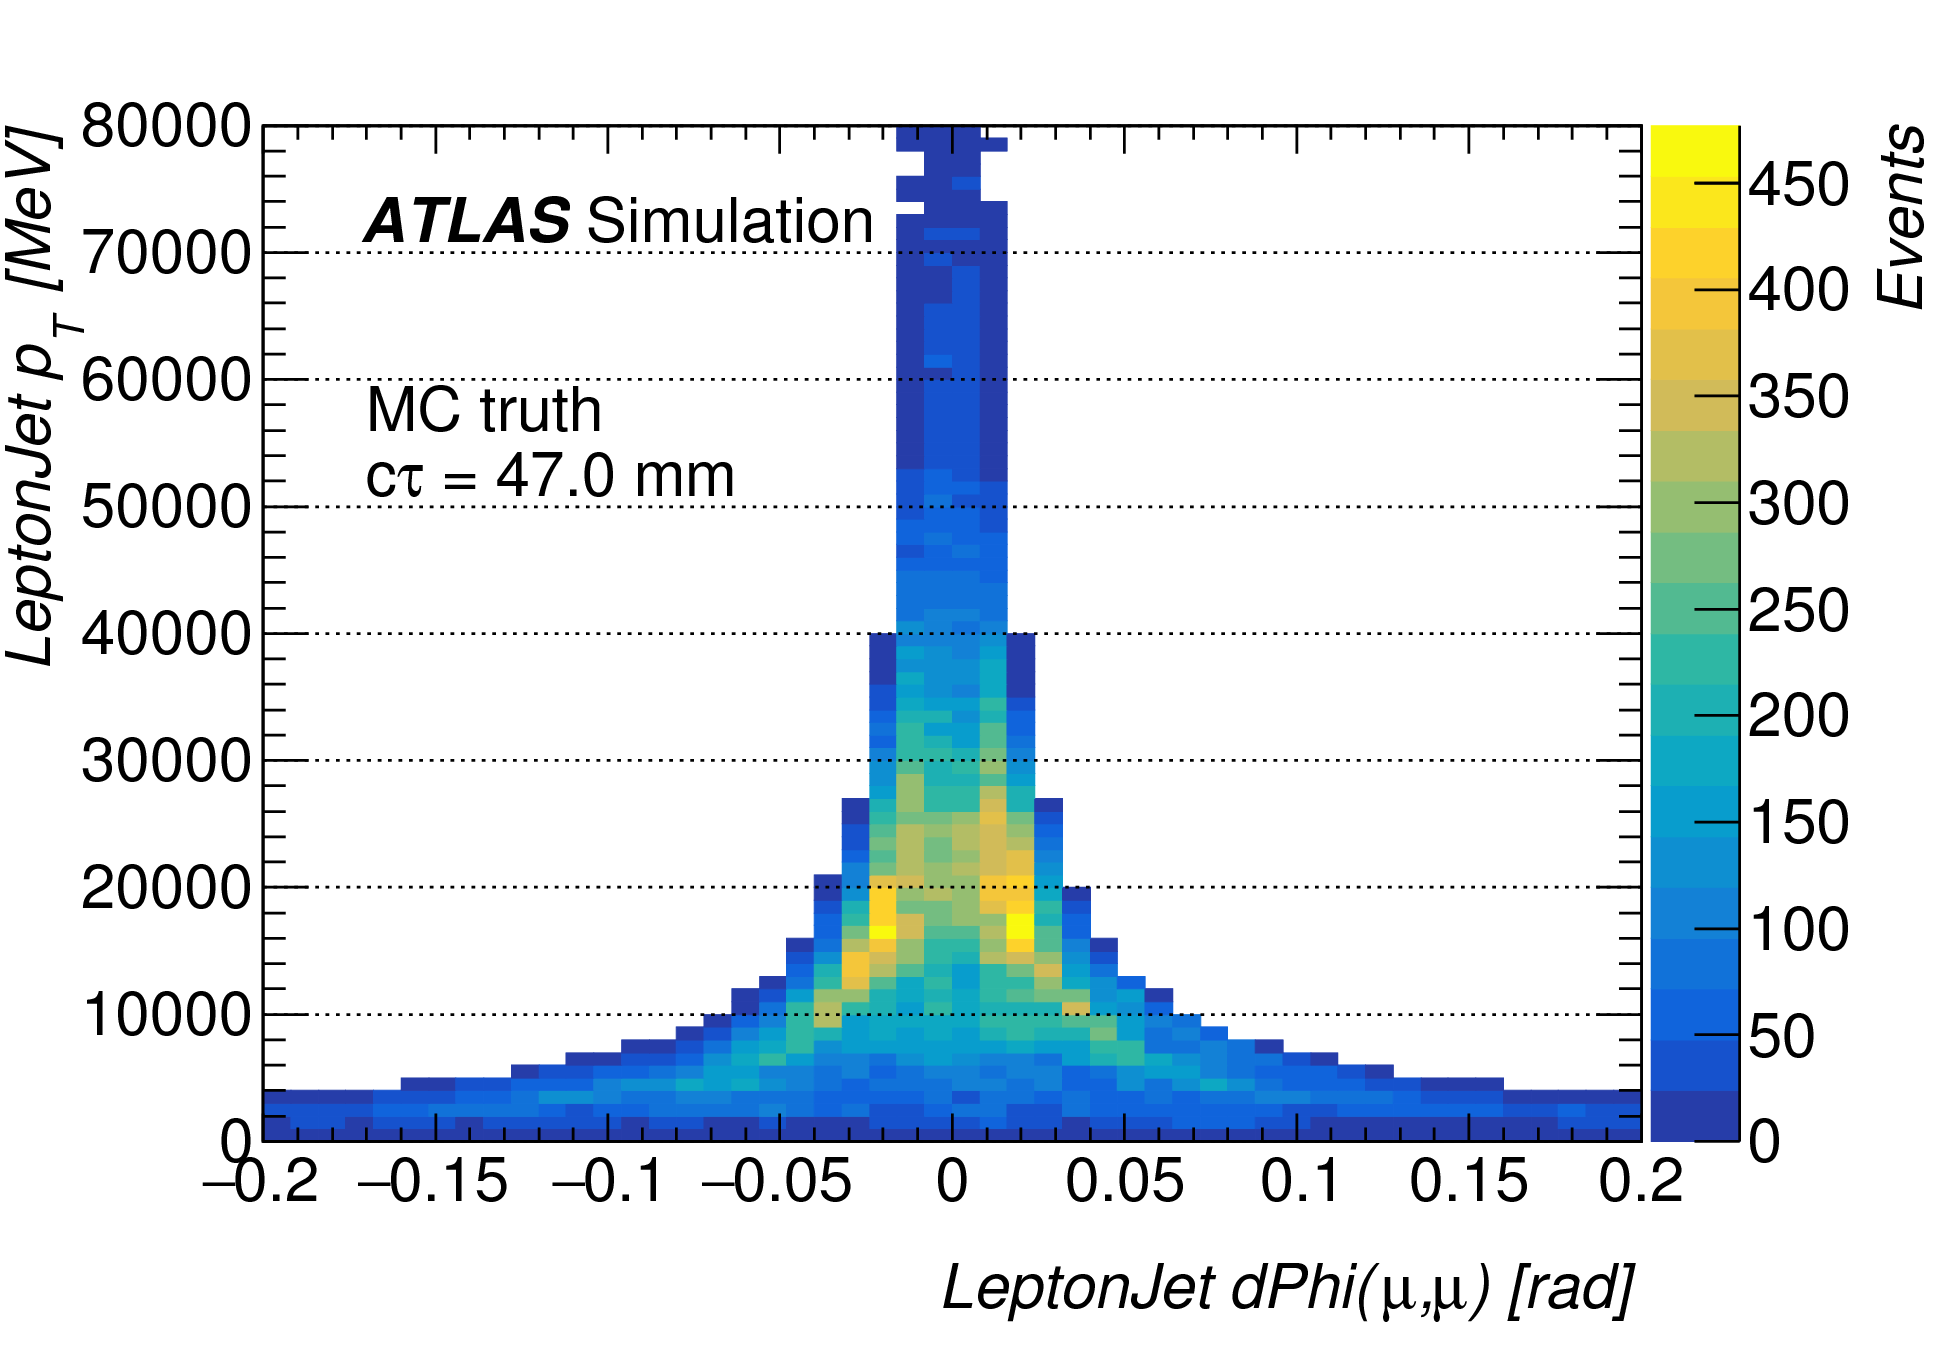
\includegraphics[width=0.7\textwidth]{figures/fig_016_anglemuons.png} 
  \caption{Opening angle between muons in a Hidden Valley model, where a sub-GeV-mass particle decays to $\mu^+\mu^-$. The opening angle is well below the resolution of the current system. }
  \label{fig:anglemuons}
\end{center}
\end{figure}

\subsubsection{Timing Detector} \label{sec:upgradetiming}

Precision timing can be provided by the aforementioned calorimetry upgrades. However, the tens of ps timing resolution in the upgraded calorimeters is only achievable for particles with energy above tens of GeV. Moreover, timing information for delayed objects from calorimetry alone will be affected by the beamspot smearing, which corresponds to about $180$~ps of uncertainty. Therefore, global event timing with the ability to reconstruct the vertex time and exploit time information in charged particle reconstruction requires a dedicated fast timing detector.

\paragraph{CMS Upgrade}

For the CMS experiment, the proposed MIP timing detector (MTD) will comprise a barrel and an endcap region made up of a single layer device between the tracker and calorimeters, and cover $|\eta|$ up to $\sim3$. In the barrel, the proposal is to adapt the present Tracker Support Tube (TST) design by instrumenting the current location of the thermal screen with a thin, actively-cooled, stand-alone detector, based on lutetium-yttrium orthosilicate crystals activated with cerium (LYSO:Ce) and read-out with silicon photomultipliers. The endcap region can be instrumented with a hermetic, single layer of MIP-sensitive silicon devices with high timing resolution, with a pseudorapidity acceptance from about $|\eta|=1.6$ to $|\eta|=2.9$. The MTD is designed to provide timing resolution of a few tens of ps for charged tracks throughout the detector lifetime. The performance projection in Section~\ref{sec:upgradesearch} is evaluated with a 30~ps resolution for a $\pt$ threshold of 0.7 GeV in the barrel and a $p$ threshold of 0.7 GeV in the endcap, and covering the expected MTD fiducial region of $|\eta| < 3$.

\paragraph{ATLAS Upgrade}

The High-Granularity Timing Detector (HGTD) is intended to distinguish between collisions occurring very close in space but well-separated in time. Currently there is not yet a TDR for this project. The current proposed detector design is based on low-gain avalanche detector technology that will cover the $|\eta|$ region between 2.4 and 4,
with a timing resolution of 30~ps for MIPs. High-precision timing will improve the track-to-vertex association in the forward region, impacting jet and lepton reconstruction, as well as offering unique capabilities for online and offline luminosity determination.

\subsubsection{Trigger} \label{sec:upgradetrigger}

The ATLAS and CMS experiments adopt a two-level trigger system:~the hardware-based Level-1 trigger (L1) and the software-based high-level trigger (HLT). 

\paragraph{CMS Upgrade}

For the CMS experiment, the L1 trigger currently only uses calorimeter and muon information. At the HL-LHC, with the aforementioned outer tracker upgrade of $\pt$ modules and stub-finding capabilities, tracking information will be included at L1~\cite{Lourenco:2283192}. The L1 track trigger uses parallel processing and pattern recognition on stub information to achieve track finding at an output rate of $750$~kHz.

The L1 tracking capability will be further complemented by the calorimeter and muon upgrades, which provide more precise position and momentum resolution, calorimeter shower shape, and more muon hits in the forward region. In the L1 trigger, the electron and photon trigger algorithms for HL-LHC will use information from the electromagnetic calorimeter as well as from the outer tracking detectors. The algorithm should preserve the ability to reconstruct electromagnetic clusters with $\pt$ above a few GeV with high efficiency ($95\%$ or greater above 10 GeV) as well as achieve high spatial resolution which should be as close as possible to the offline reconstruction. Following the upgrade of both on-detector and off-detector electronics for the barrel calorimeters at the HL-LHC, the EB 
will provide energy measurements with a granularity of (0.0174, 0.0174)
in $(\eta, \phi)$, as opposed to the current input to the L1 trigger consisting of trigger towers with a granularity of (0.087, 0.087). The much finer granularity and resulting improvement in position resolution of the electromagnetic trigger algorithms is critical in improving electron/photon trigger efficiency and suppressing background at high pile-up.

The L1 Global Trigger (GT) will be upgraded with more sophisticated and effective global trigger calculations based on topology, plus an additional intermediate Correlator Trigger (CT) to fully exploit the increased information in the trigger objects, such as matching tracking info with finely-grained calorimeter information, or a combination of muon and track information. The upgraded detector readout and DAQ systems will allow $12.5\,\, \mu \mathrm{s}$ latency and a L1 rate of 750~KHz; the latter may be substantially reduced by adding L1 tracking information matched to improved L1 trigger objects from the calorimeters and muon system. At the high-level trigger (HLT), the processing power is expected to scale up by pile-up and L1 rate, with an output rate of $7.5$~kHz and up to $10$~kHz.

\paragraph{ATLAS Upgrade}

{\bf \textcolor{red}{[JB: Can this section be expanded?  It would be great to provide a bit more detail about all of the things mentioned, to allow for a clearer comparison to the CMS plans.]}}

\noindent {\bf \textcolor{red}{[BS: ATLAS L0 is mentioned earlier in the paper but it is not mentioned in the trigger section.]}}

\noindent {\bf \textcolor{red}{[BS: ATLAS FTK doesn't seem to be mentioned at all?]}}

The ATLAS trigger and the data acquisition system are being planned with the intention of fully exploiting the physics potential of the HL-LHC. A baseline architecture, based on a single-level hardware trigger with a maximum rate of 1~MHz and 10~$\mu$s latency, is proposed and documented in Ref.~\cite{Collaboration:2285584}. 
With the help of a hardware-based tracking sub-system as co-processor, software-based reconstruction follows to achieve further rejection. Up to 10~kHz event data are sent into storage.

The upgraded trigger system will take advantage of increased granularity provided by the calorimeters, will improve efficiency for muon-based triggers and perform hardware-based tracking profiting from the extended coverage of the planned Inner Tracker (ITk).

\subsection{Object Performance: Tracking and Vertexing} \label{sec:upgradeobject}

The ability of the detectors to reconstruct tracks and find vertices with high precision and efficiency in a high-density environment underlies the experimental reach for displaced objects. This section reviews the ATLAS and CMS experiments' projected tracking performance at the HL-LHC, highlighting improvements and new features with the upgrades.

\subsubsection{CMS Performance}

\paragraph{L1 Tracking}

With the aforementioned tracker and L1 track trigger upgrades, the CMS experiment will be able to do track finding at L1 as well as offline at HL-LHC. Both L1 and offline tracking performance are discussed here.

All L1 tracking studies have been performed assuming 3~GeV stub $\pt$ thresholds. In Figure~\ref{fig:cmsL1lepton}, the L1 tracking efficiency for prompt muons and electrons for \ttbar~events in a scenario with 200 pile-up interactions per bunch crossing, on average, is presented. The tracking efficiency for muons exhibits a sharp turn-on at the 3~GeV stub $\pt$ threshold, and saturates at approximately $98\%$. The tracking efficiency for electrons turns on more slowly and flattens out at $90\%$, mostly due to interaction with the detector material.

In Figure~\ref{fig:cmsL1tracks}, the L1 tracking resolutions of the $\pt$ and $z_0$ parameters of muons with $\pt > 10$~GeV in \ttbar~events is shown for various average pile-up scenarios. The resolutions are defined in terms of an interval centered on the residual distribution that contains $68\%$ or $90\%$ of the tracks. Loss in tracking efficiency due to truncation effects (where there is insufficient time to transfer all the stub data) is determined from hardware and emulation to be at the level of 10$^{-3}$ when considering \ttbar~samples with a pile-up rate of 200. As expected, resolutions degrade at forward pseudorapidity due to a corresponding increase in multiple scattering. In general, L1 parameter resolutions are excellent, which will provide for robust trigger object matching and charged particle reconstruction in the L1 trigger.

\begin{figure}[t]
\begin{center}
  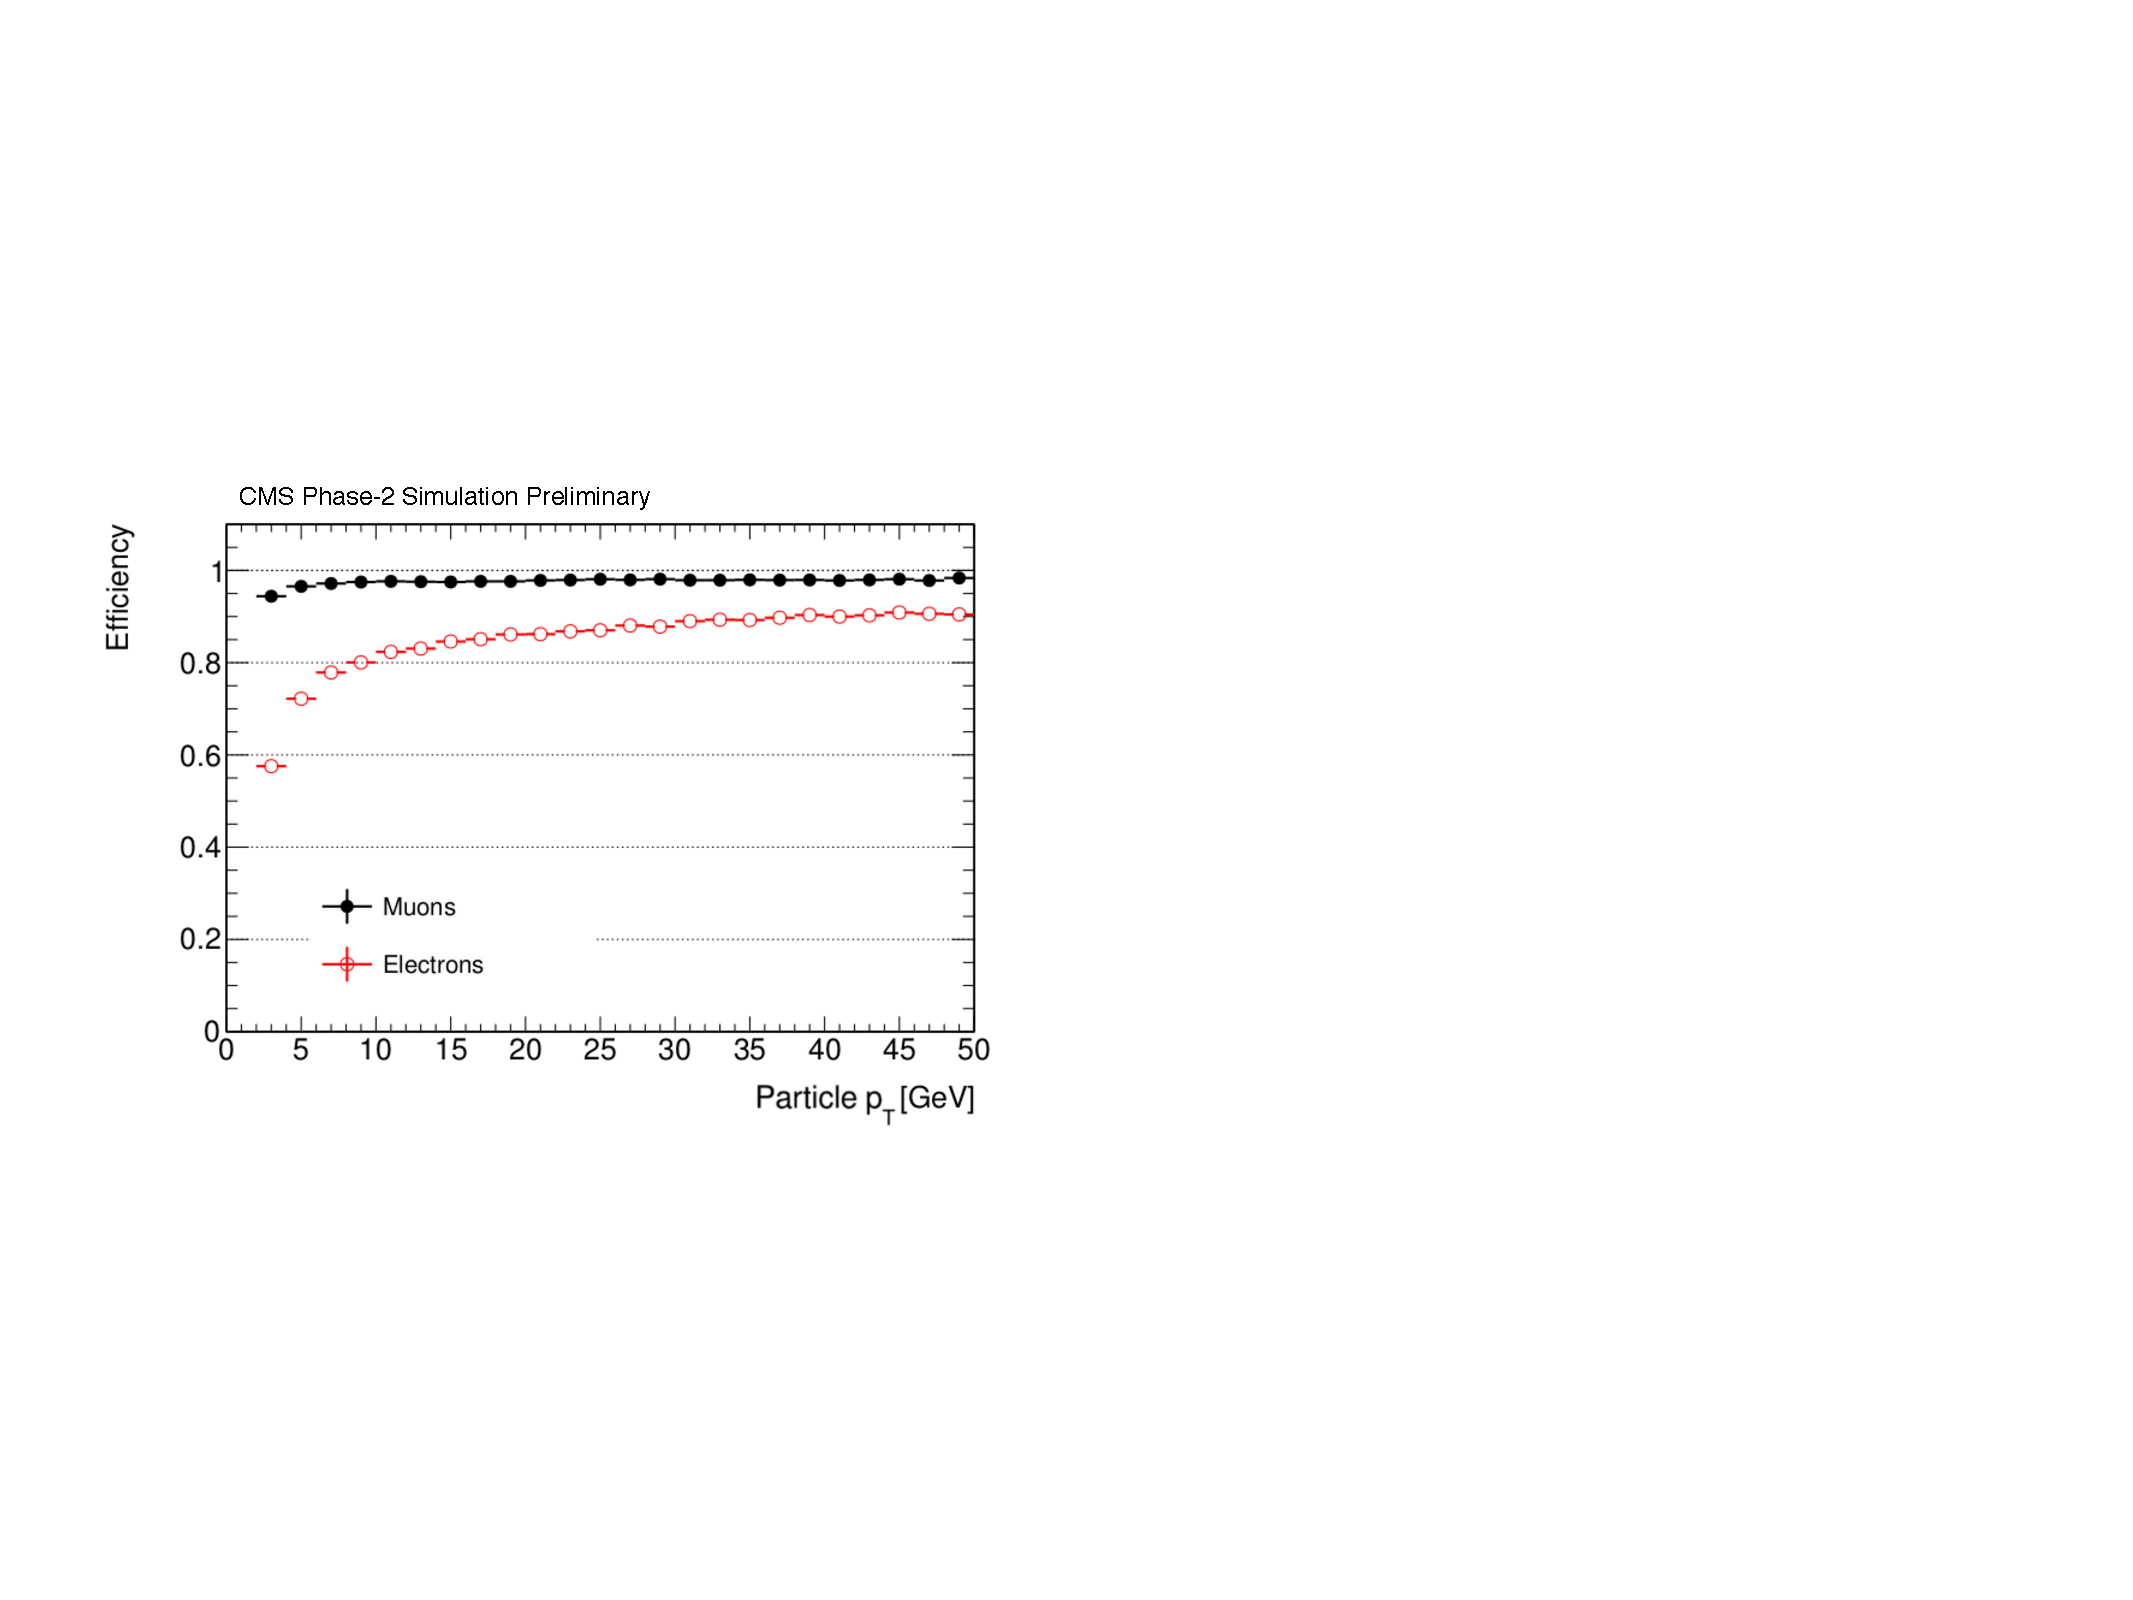
\includegraphics[width=0.47\textwidth]{figures/cmsupgrade/TDR-17-001_fig6_6_a.pdf} \hfill
  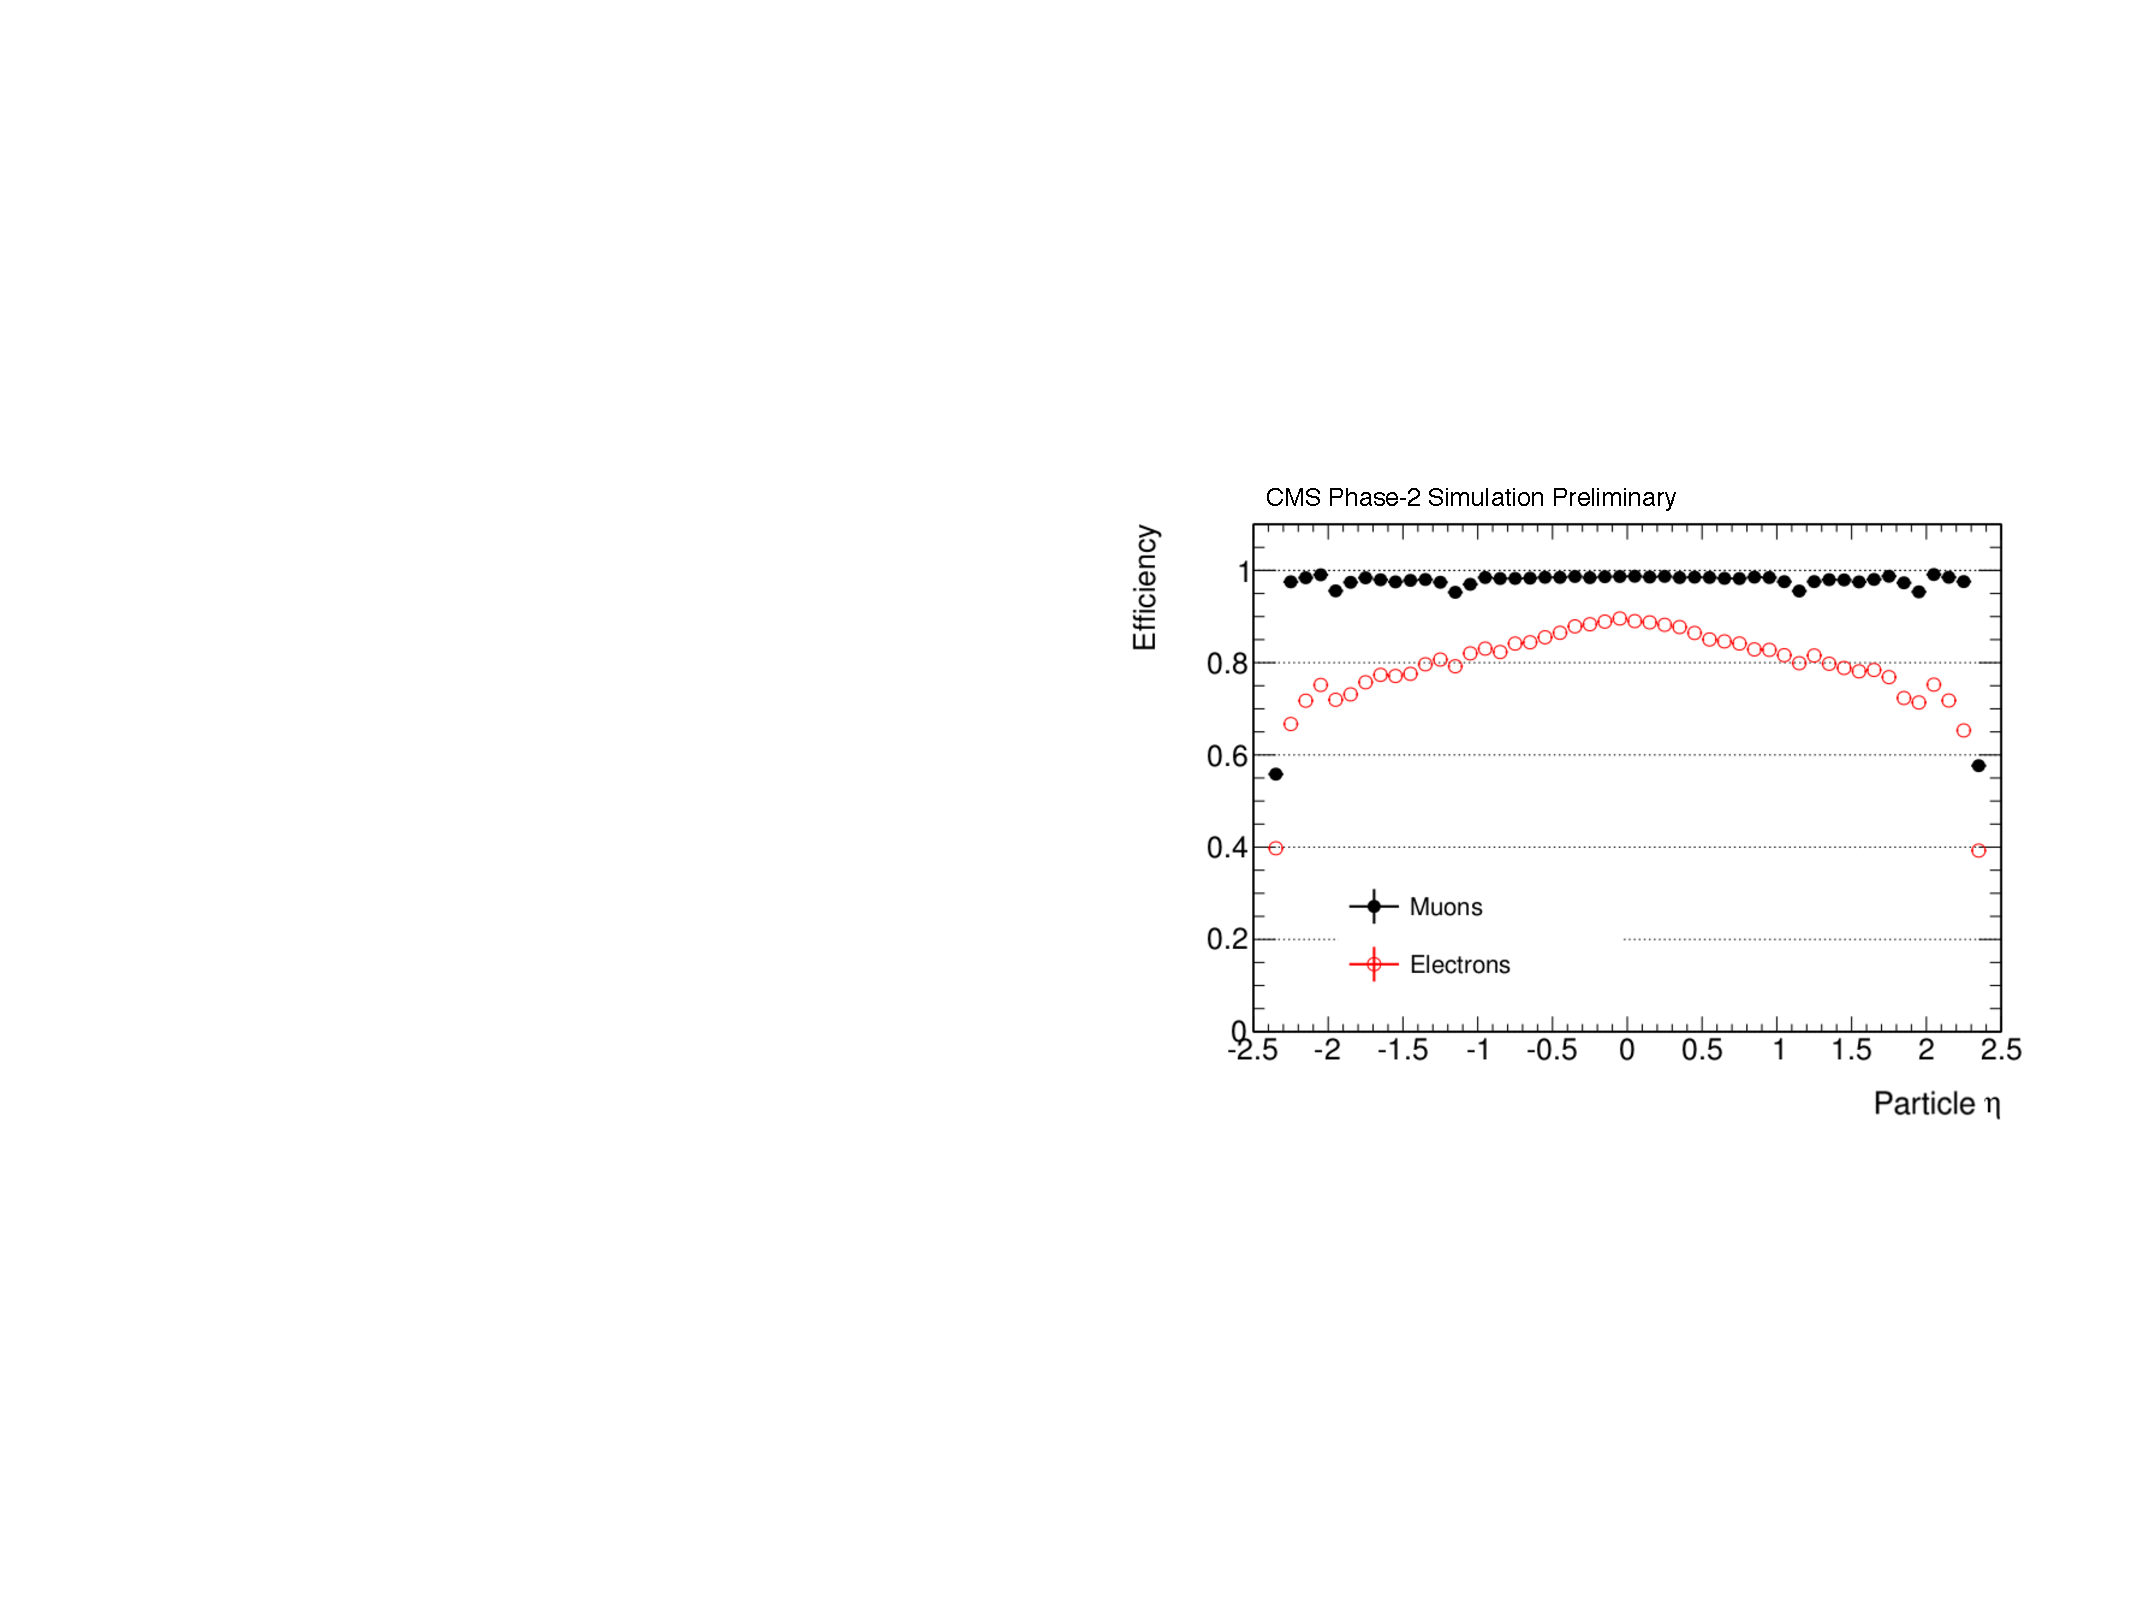
\includegraphics[width=0.47\textwidth]{figures/cmsupgrade/TDR-17-001_fig6_6_b.pdf}
  \caption{{\bf Left:}~L1 tracking efficiency versus generated particle $\pt$ for $|\eta| < 2.4$.
	{\bf Right:}~L1 tracking efficiency versus $\eta$ for $\pt > 3$~GeV. Results for muons (electrons) are shown as filled black (open red) circles, and are produced with \ttbar~events in a scenario with 200 pile-up events per bunch crossing, on average~\cite{Collaboration:2272264}. }
  \label{fig:cmsL1lepton}
\end{center}
\end{figure}

\begin{figure}[t]
\begin{center}
  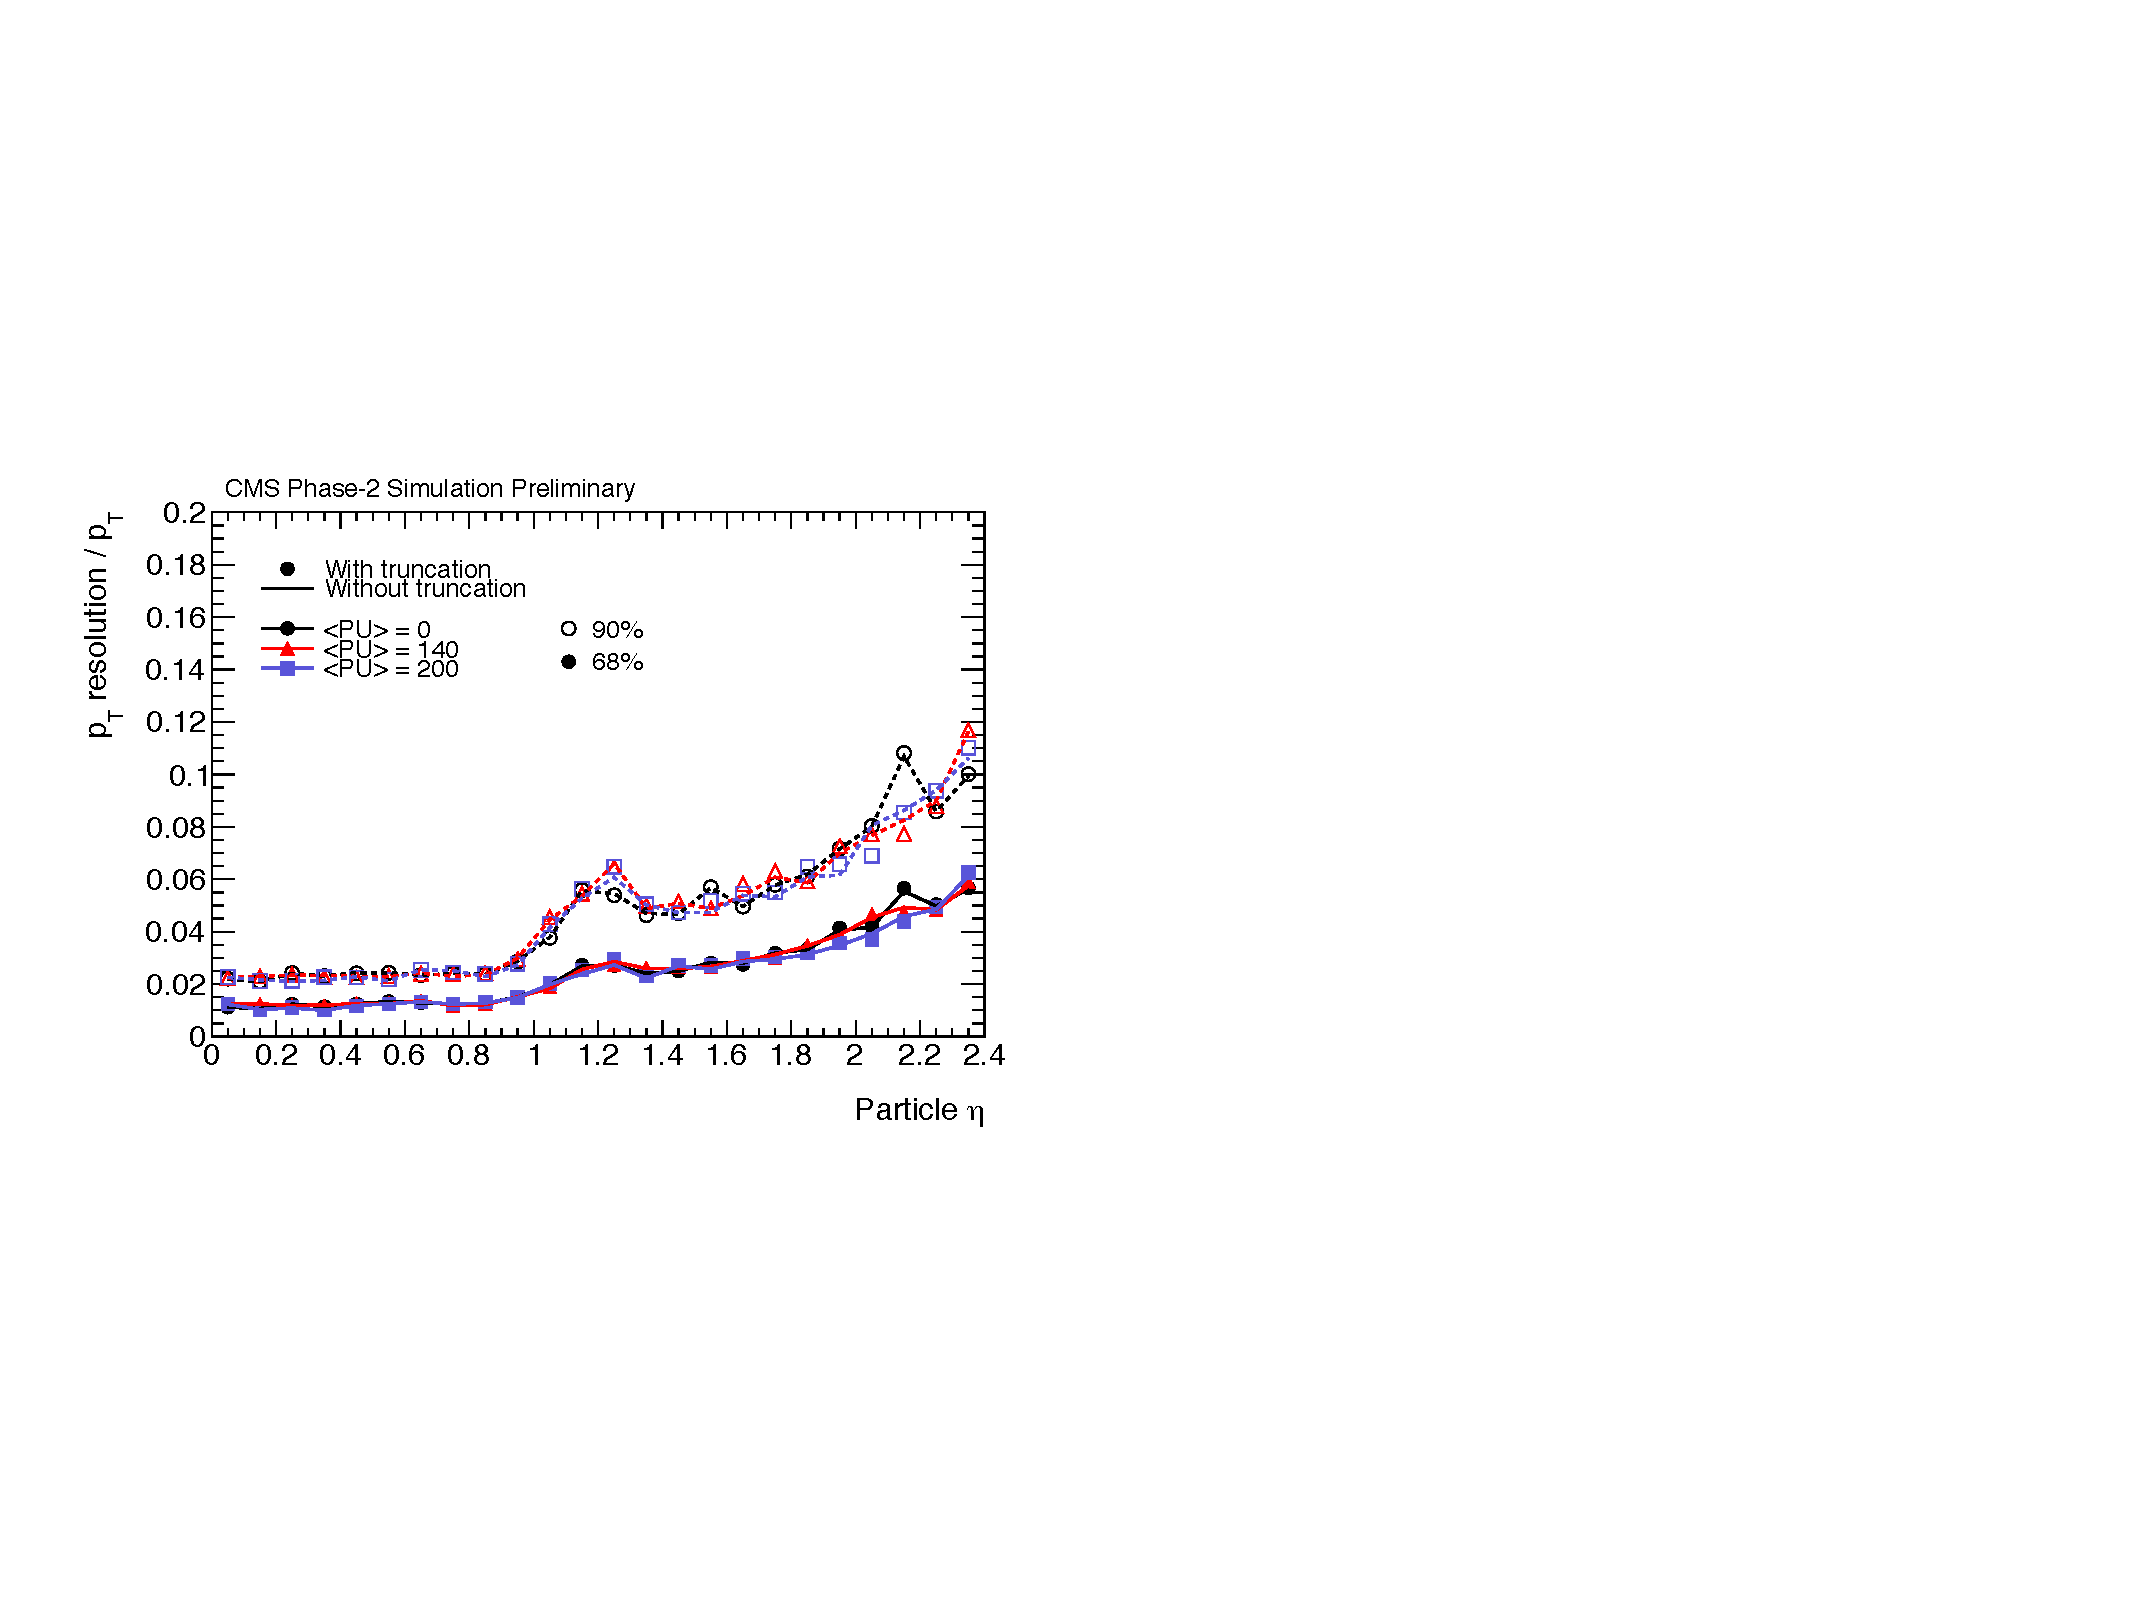
\includegraphics[width=0.47\textwidth]{figures/cmsupgrade/TDR-17-001_fig6_8_a.pdf} \hfill
  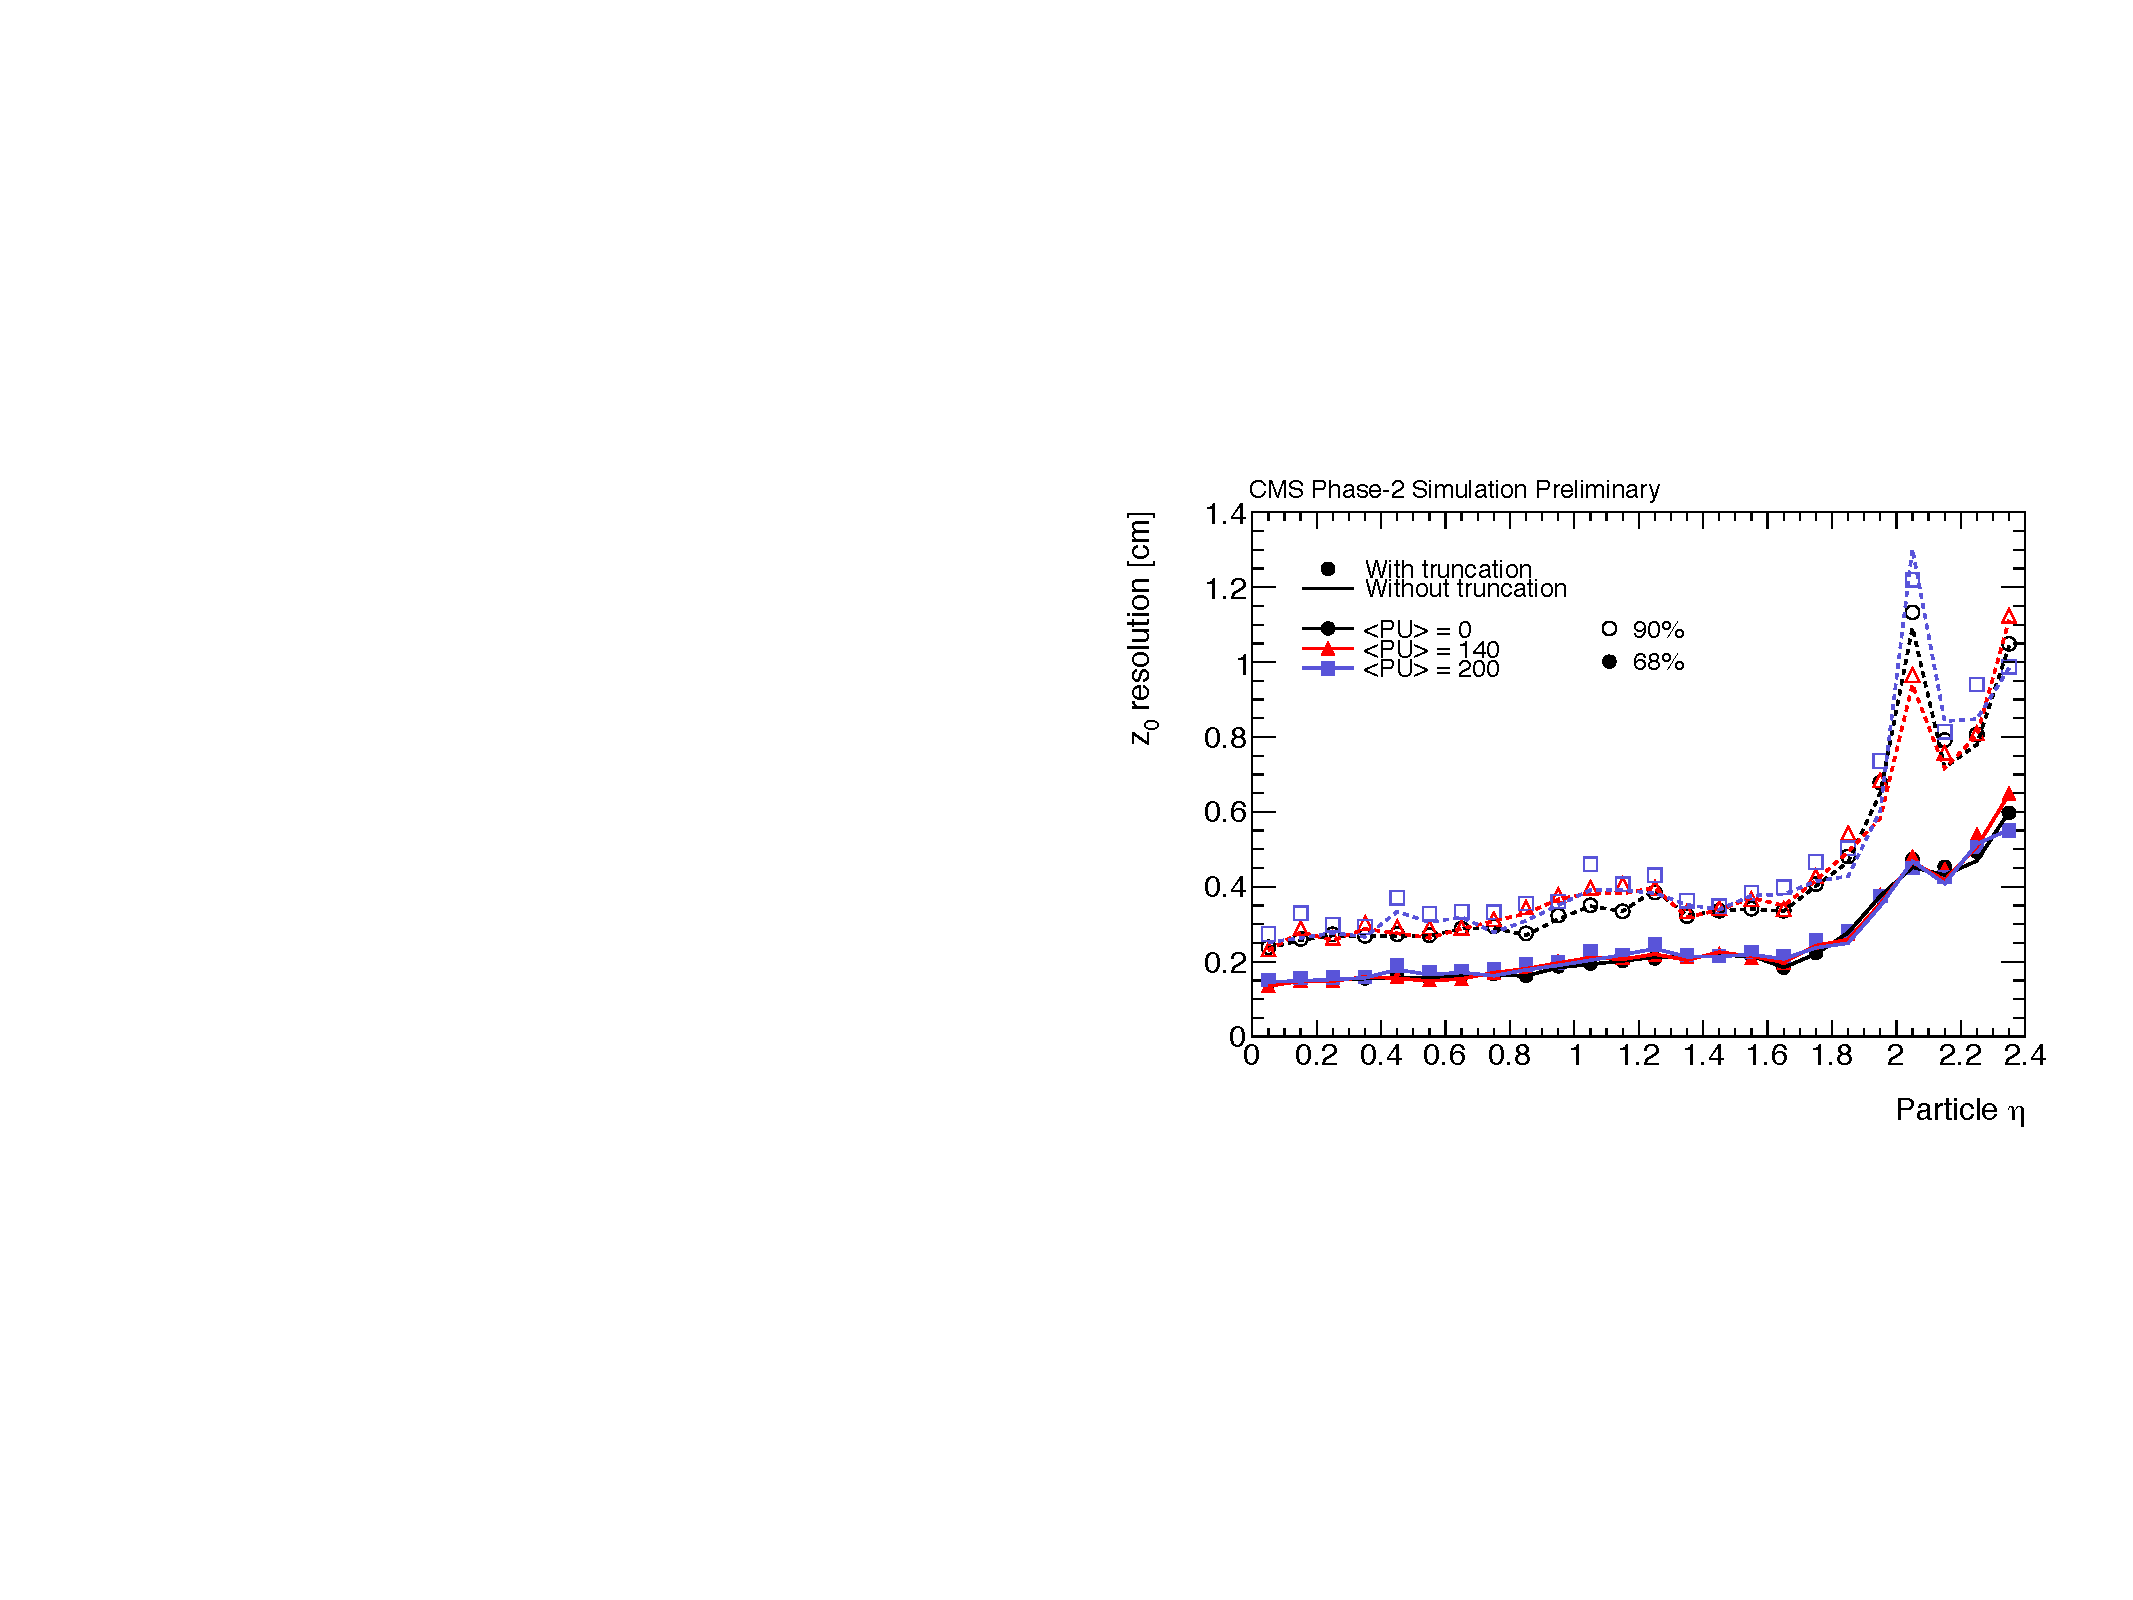
\includegraphics[width=0.47\textwidth]{figures/cmsupgrade/TDR-17-001_fig6_8_b.pdf}
  \caption{ Relative $\pt$ (left) and $z_0$ resolution versus pseudorapidity for muons in \ttbar~events with zero (black dots), 140 (red triangles), and 200 (blue squares) pile-up events per bunch crossing, on average. Results are shown for scenarios in which truncation effects are (markers) or are not (lines) considered in the emulation of L1 track processing. The resolutions correspond to intervals in the track parameter distributions that encompass $68\%$ (filled markers and solid lines) or $90\%$ (open markers and dashed lines) of all tracks with $\pt > 3$~GeV~\cite{Collaboration:2272264}.}
  \label{fig:cmsL1tracks}
\end{center}
\end{figure}

\paragraph{Offline Tracking}

Preliminary results on the offline tracking performance over the full acceptance of the CMS tracker are excellent, with further improvements expected as the detector design and simulation algorithms are optimized. In Figure~\ref{fig:cmstrackres}, the resolution of the transverse momentum and the transverse impact parameter for single muons with $\pt = 10$~GeV as a function of the pseudorapidity, both with the current detector and after the implementation of the HL-LHC upgrades, is shown. The better hit resolution of the HL-LHC tracker and the reduction of the material budget result in a significantly improved $\pt$ resolution. The transverse impact parameter resolution is also improved with respect to the current detector, ranging from below $10\,\,\mu\mathrm{m}$
in the central region to about $20\,\,\mu\mathrm{m}$ at the edge of the acceptance.

\begin{figure}[t]
\begin{center}
  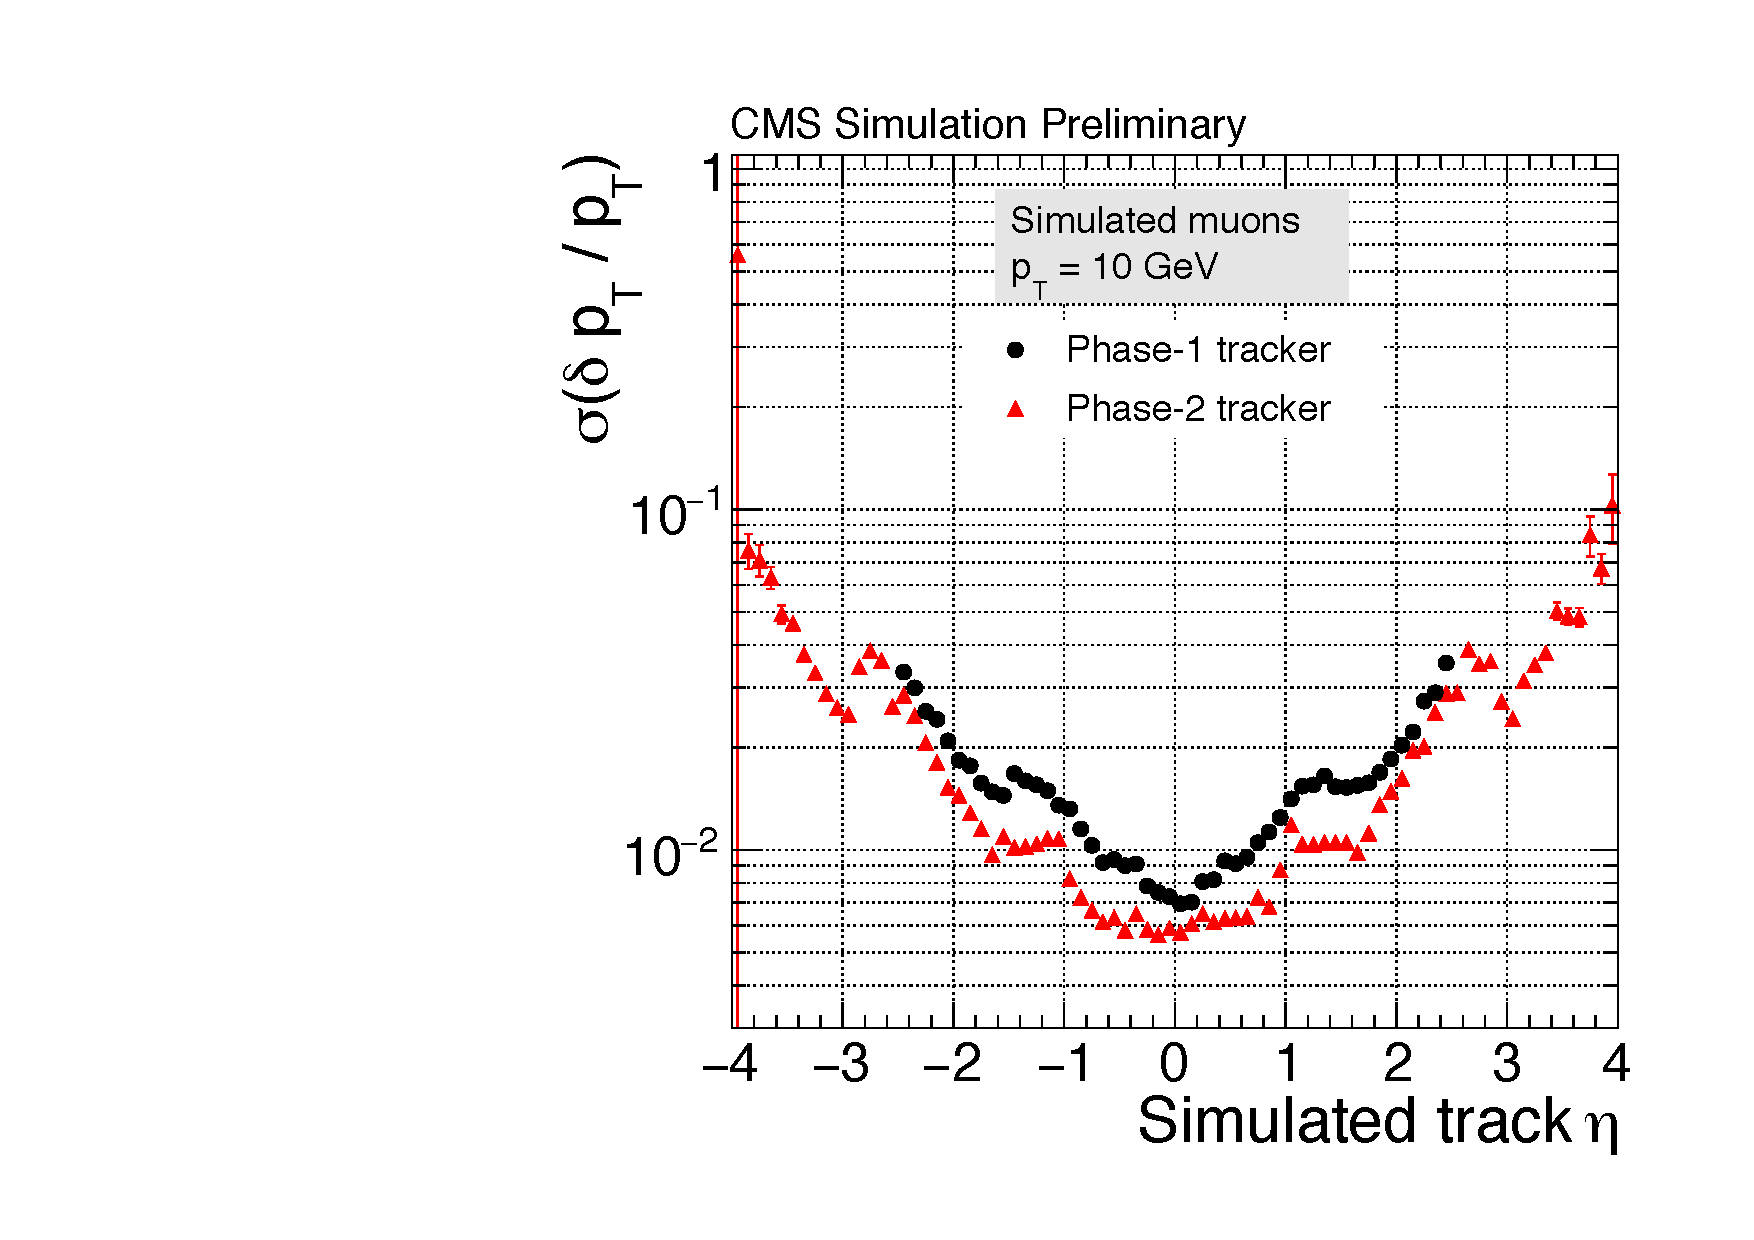
\includegraphics[width=0.47\textwidth]{figures/cmsupgrade/TDR-17-001_fig6_12_a_ptres_vs_eta_Sigma_vsPhase1.pdf} \hfill
  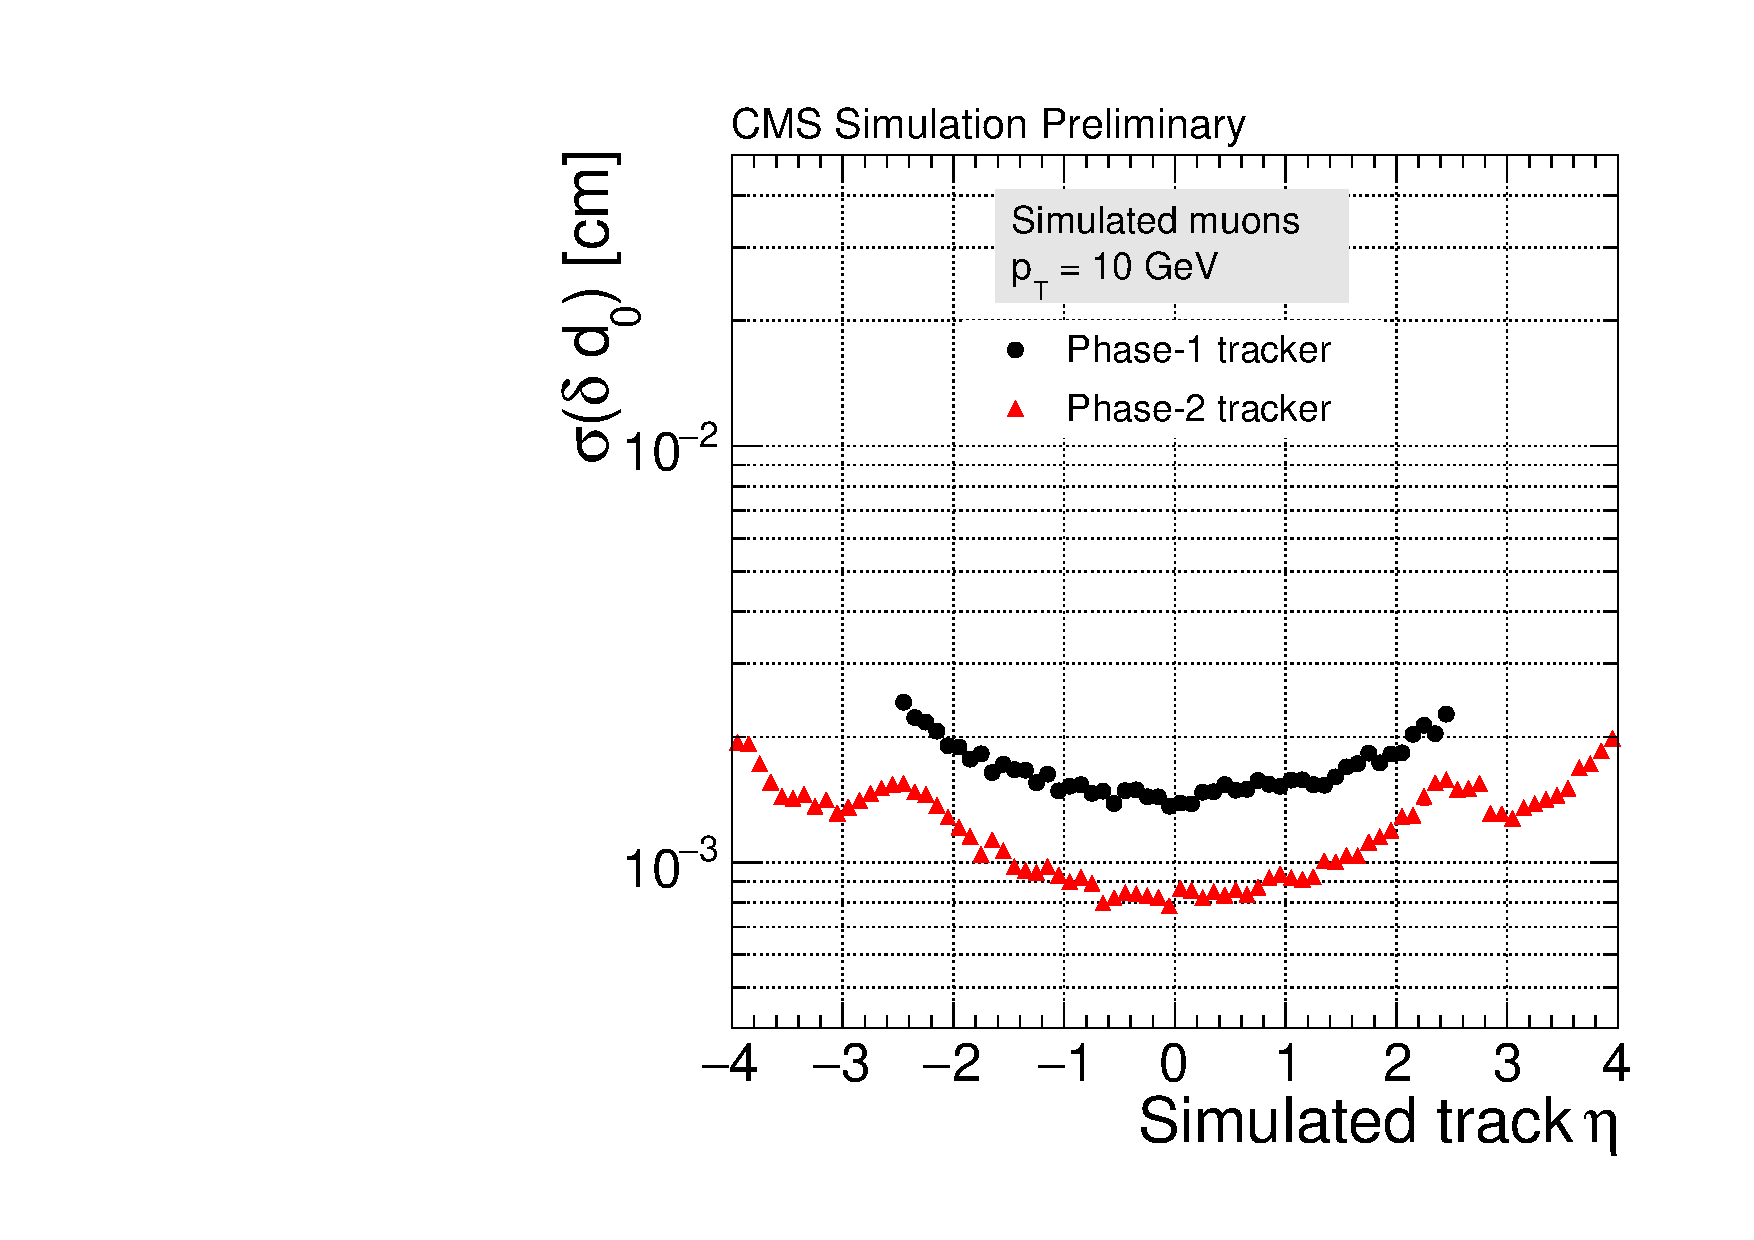
\includegraphics[width=0.47\textwidth]{figures/cmsupgrade/TDR-17-001_fig6_12_b_dxyres_vs_eta_Sigma_vsPhase1.pdf}
  \caption{Relative resolution of the transverse momentum (left) and transverse impact parameter (right) as a function of the pseudorapidity for the current (black dots) and the upgraded (red triangles) CMS tracker, using single isolated muons with a transverse momentum of $10$~GeV~\cite{Collaboration:2272264}.}
  \label{fig:cmstrackres}
\end{center}
\end{figure}

For \ttbar~events, the efficiency to identify the primary vertex correctly is $\sim 95\%$ at an average pile-up level of 140, and $\sim93\%$ at an average pile-up level of 200. The vertex algorithm used is the same as the one used in Run 2 for a pile-up of about 35, therefore it is not yet optimized for vertex reconstruction at very high pile-up. In Figure~\ref{fig:cmsvertex} the resolution of the vertex position in the $x$, $y$, and $z$ coordinates is shown as a function of the number of tracks associated to the vertex. The vertex position resolution is almost independent of the amount of pile-up in the event and the longitudinal resolution is only $50\%$ worse than the transverse one, as expected given the pixel dimensions of the inner tracker modules.

\begin{figure}[t]
\begin{center}
  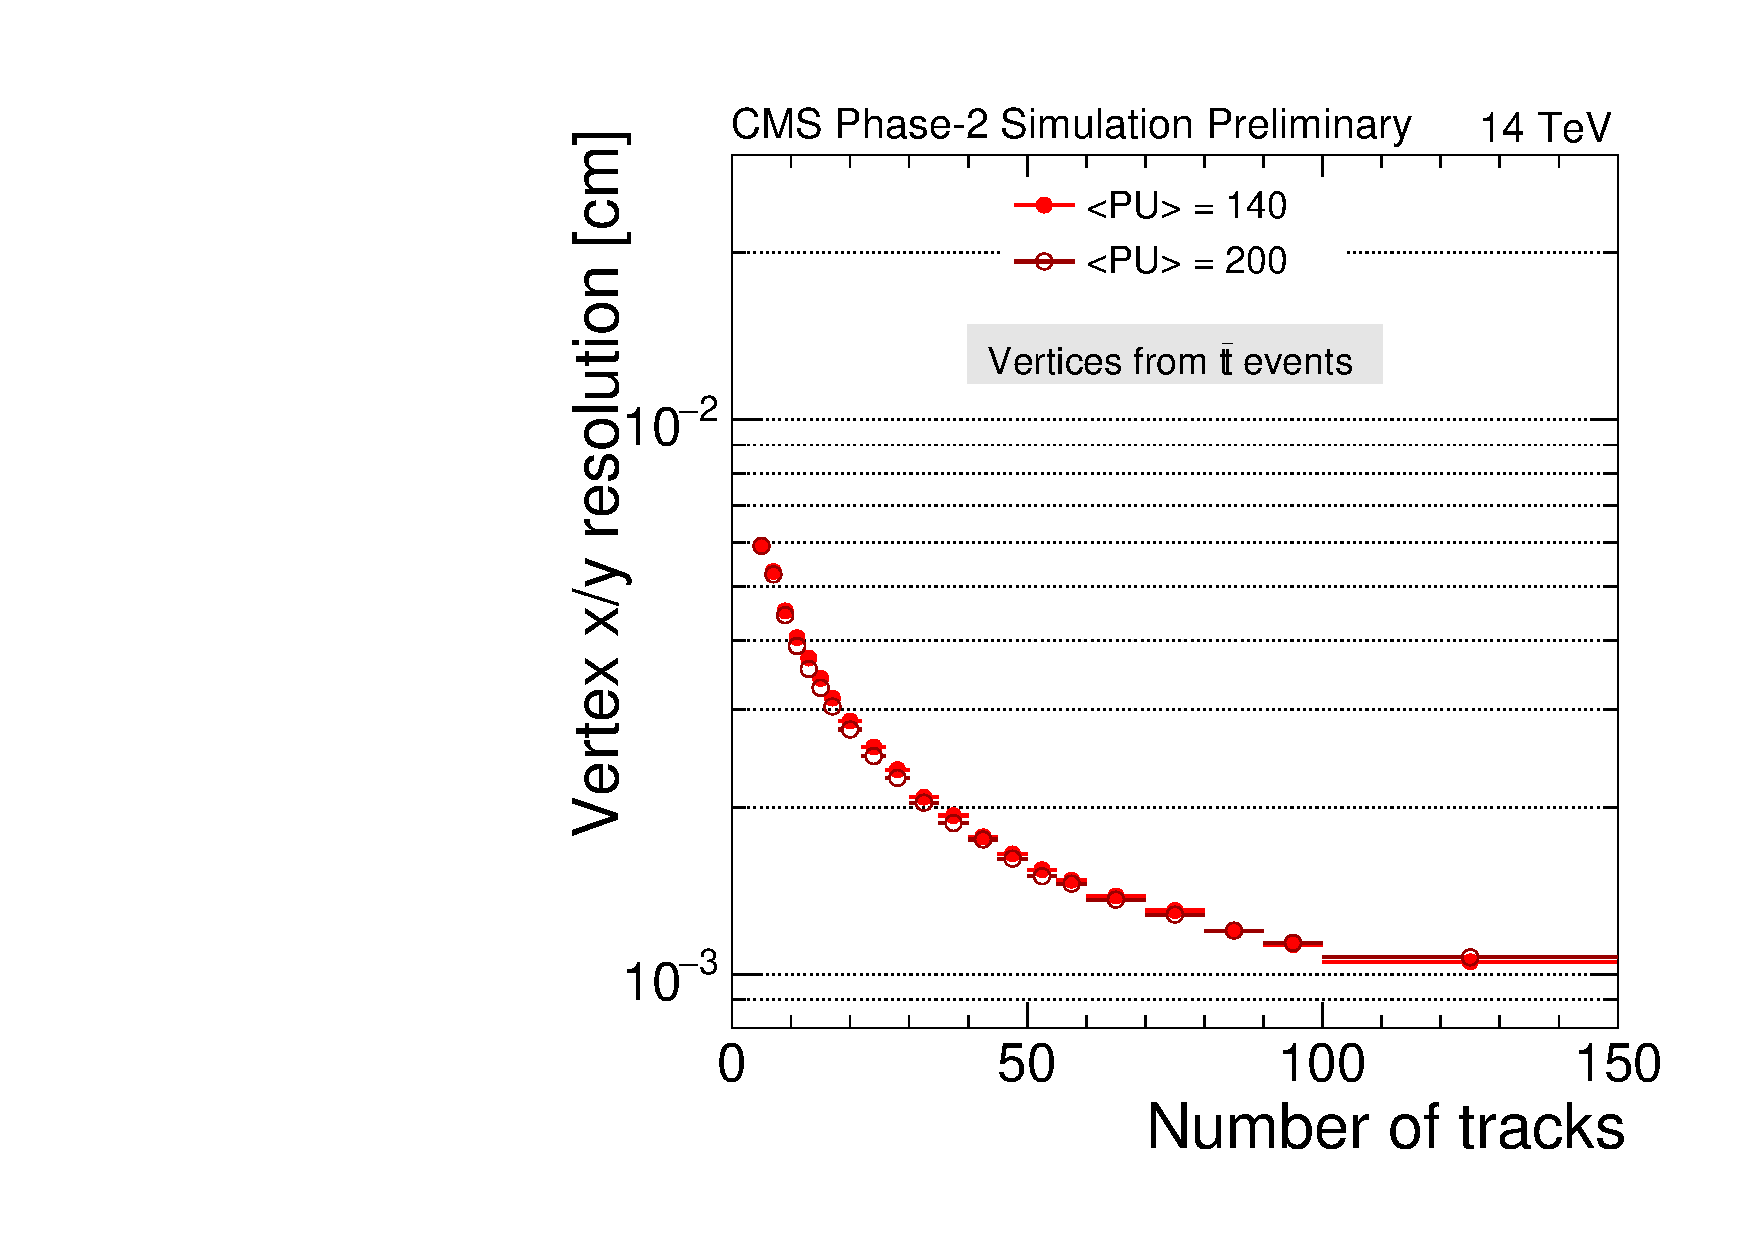
\includegraphics[width=0.47\textwidth]{figures/cmsupgrade/TDR-17-001_fig6_13_a_RecoAllAssoc2GenMatched_ResolX_vs_NumTracks_Sigma_PU.pdf} \hfill
  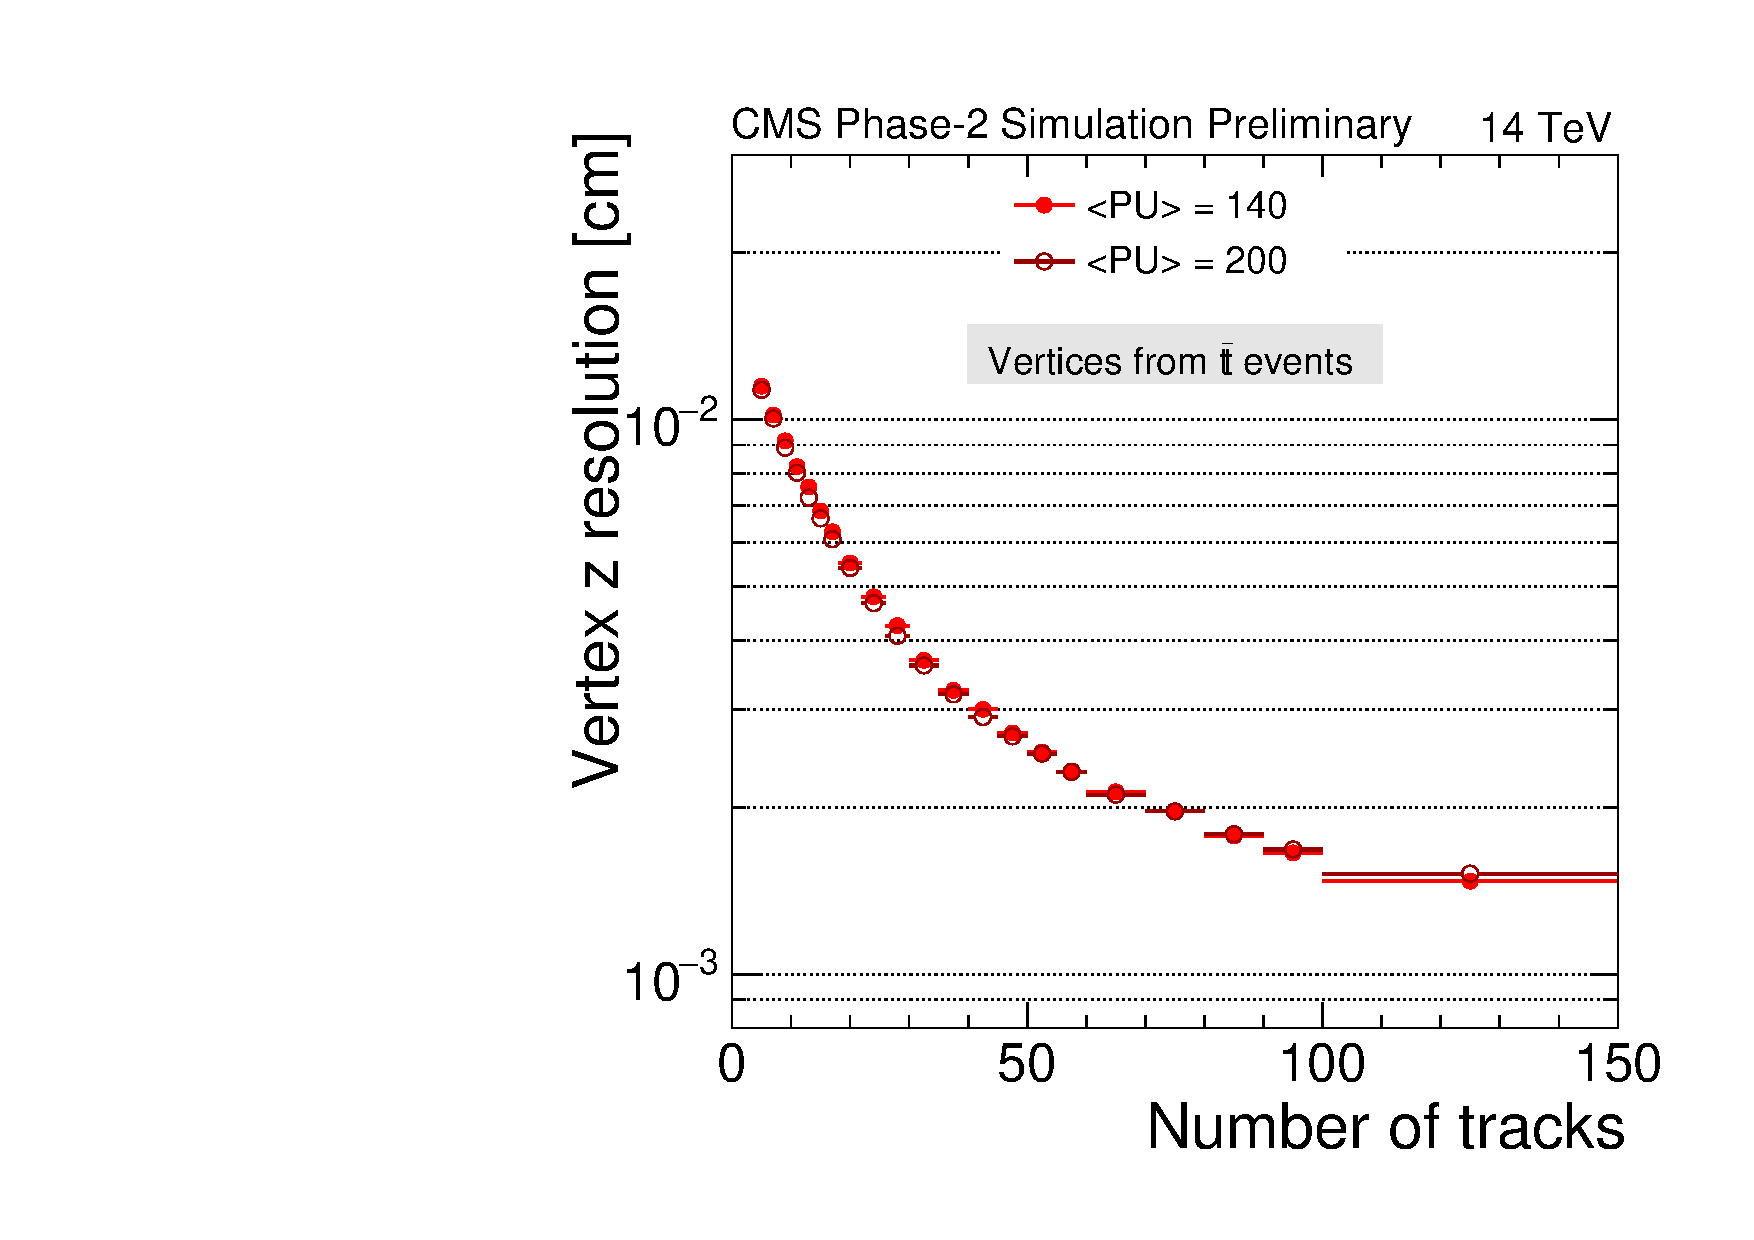
\includegraphics[width=0.47\textwidth]{figures/cmsupgrade/TDR-17-001_fig6_13_b_RecoAllAssoc2GenMatched_ResolZ_vs_NumTracks_Sigma_PU.pdf}
  \caption{Vertex position resolution in $x$ and $y$ (left) and $z$ (right) as a function of the number of tracks associated to the vertex, for \ttbar~events with an average of 140 (full circles) and 200 (open circles) pile-up interactions per bunch crossing~\cite{Collaboration:2272264}.
 }
  \label{fig:cmsvertex}
\end{center}
\end{figure}

Given that the CMS HLT tracking is based on the offline tracking code, a similar level of performance is expected.
Because of HLT time constraints, a parallelization of the algorithms is already under development and will be applied also in the HLT track reconstruction at HL-LHC.

\subsubsection{ATLAS Performance}


Excellent tracking performance is also expected with the Inner Tracker (ITk) upgrade of the ATLAS experiment for the HL-LHC era.
The left panel of Figure~\ref{fig:atlastrackeff} shows the track reconstruction efficiency for jets in $Z'\to\bar{t}t$ events with 200 pile-up for different $\eta$ ranges. The right panel of Figure~\ref{fig:atlastrackeff} shows the fake rate for reconstructed tracks in $t\bar t$ events, and there is clearly substantial improvement over the Run 2 detector performance along with the improved coverage in the forward region.

\begin{figure}[t]
\begin{center}
  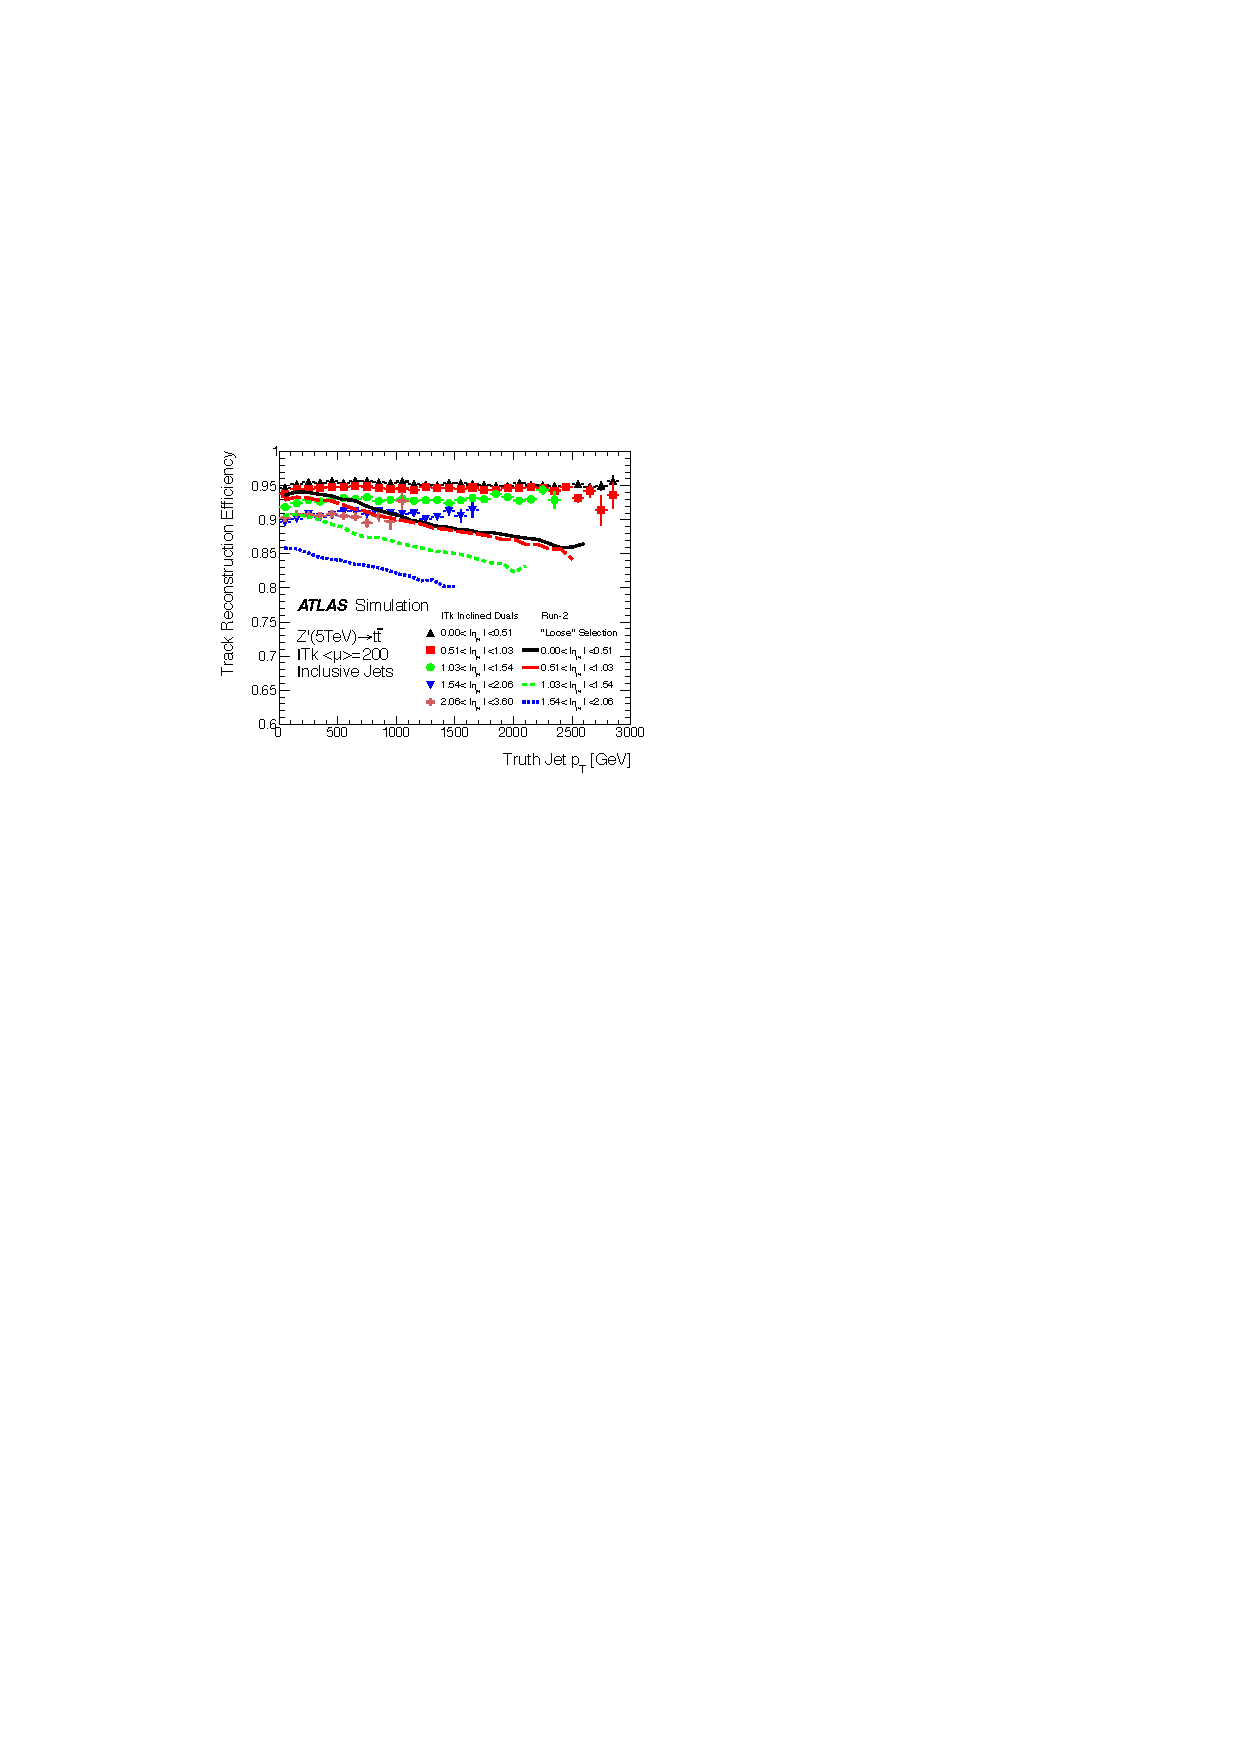
\includegraphics[width=0.47\textwidth]{figures/atlas-tdr-030-fig3-14b.pdf}
    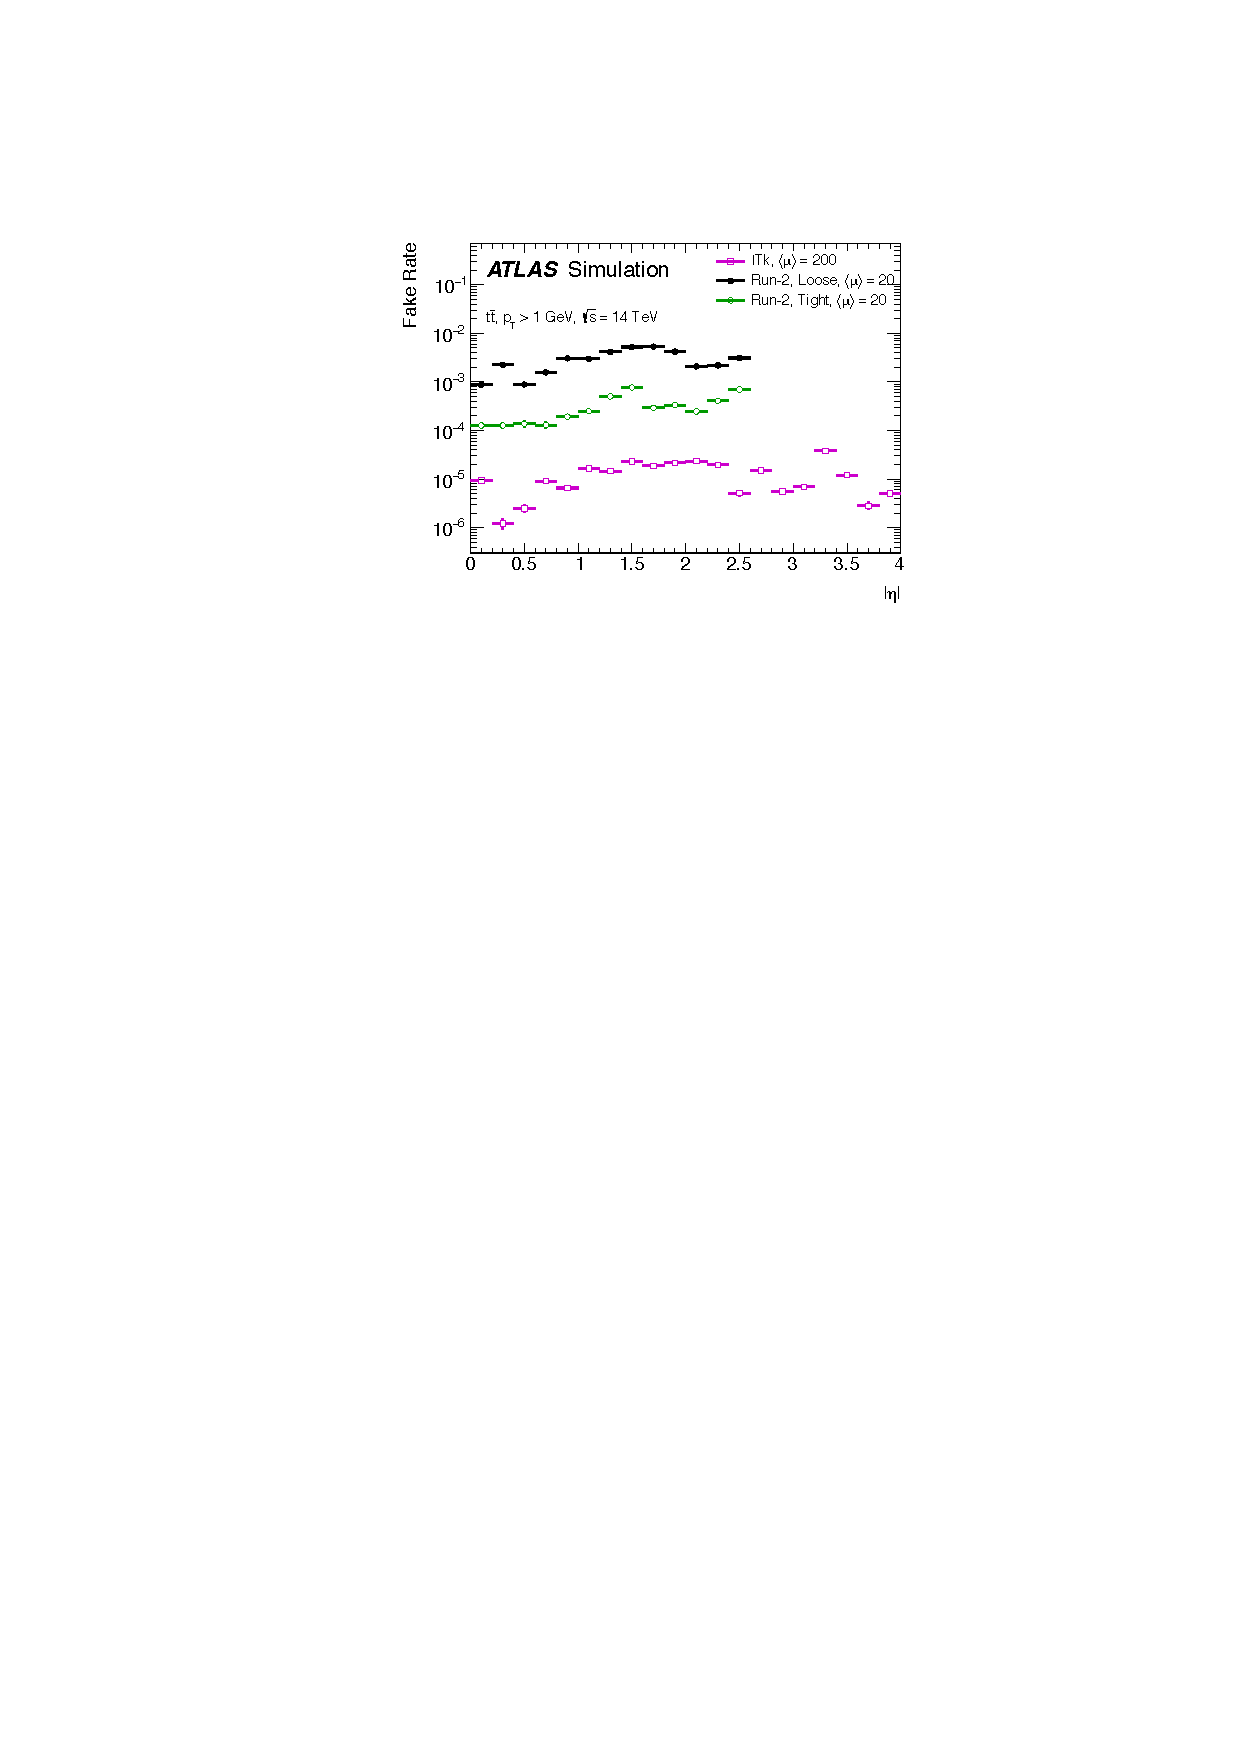
\includegraphics[width=0.47\textwidth]{figures/atlas-tdr-030-fig3-5.pdf}
  \caption{{\bf Left:} Track reconstruction efficiency for tracks in jets from $Z'\rightarrow t\bar t$ with 200 average pile-up events. The efficiency is shown as a function of jet $\pt$ for different $\eta$ ranges, and $M_{Z'}=5$ TeV. {\bf Right:} Fake rate for tracks in $t\bar t$ events with 200 average pile-up events using ITk; Run 2 detector results are shown for comparison. Both figures are from Ref.~\cite{Collaboration:2285585}.}
  \label{fig:atlastrackeff}
\end{center}
\end{figure}


In Figure~\ref{fig:atlastrackres}, the resolution of the transverse momentum and the longitudinal impact parameter for single muons with various $\pt$ values is shown as a function of the pseudorapidity both with the current
detector and projections for after the HL-LHC upgrade using digital clustering to find the tracks. The improvement is even more marked with analogue clustering:~the transverse and longitudinal impact parameter resolutions are shown for different pixel pitches in Figure~\ref{fig:atlastrackanalog}.



\begin{figure}[t]
\begin{center}
  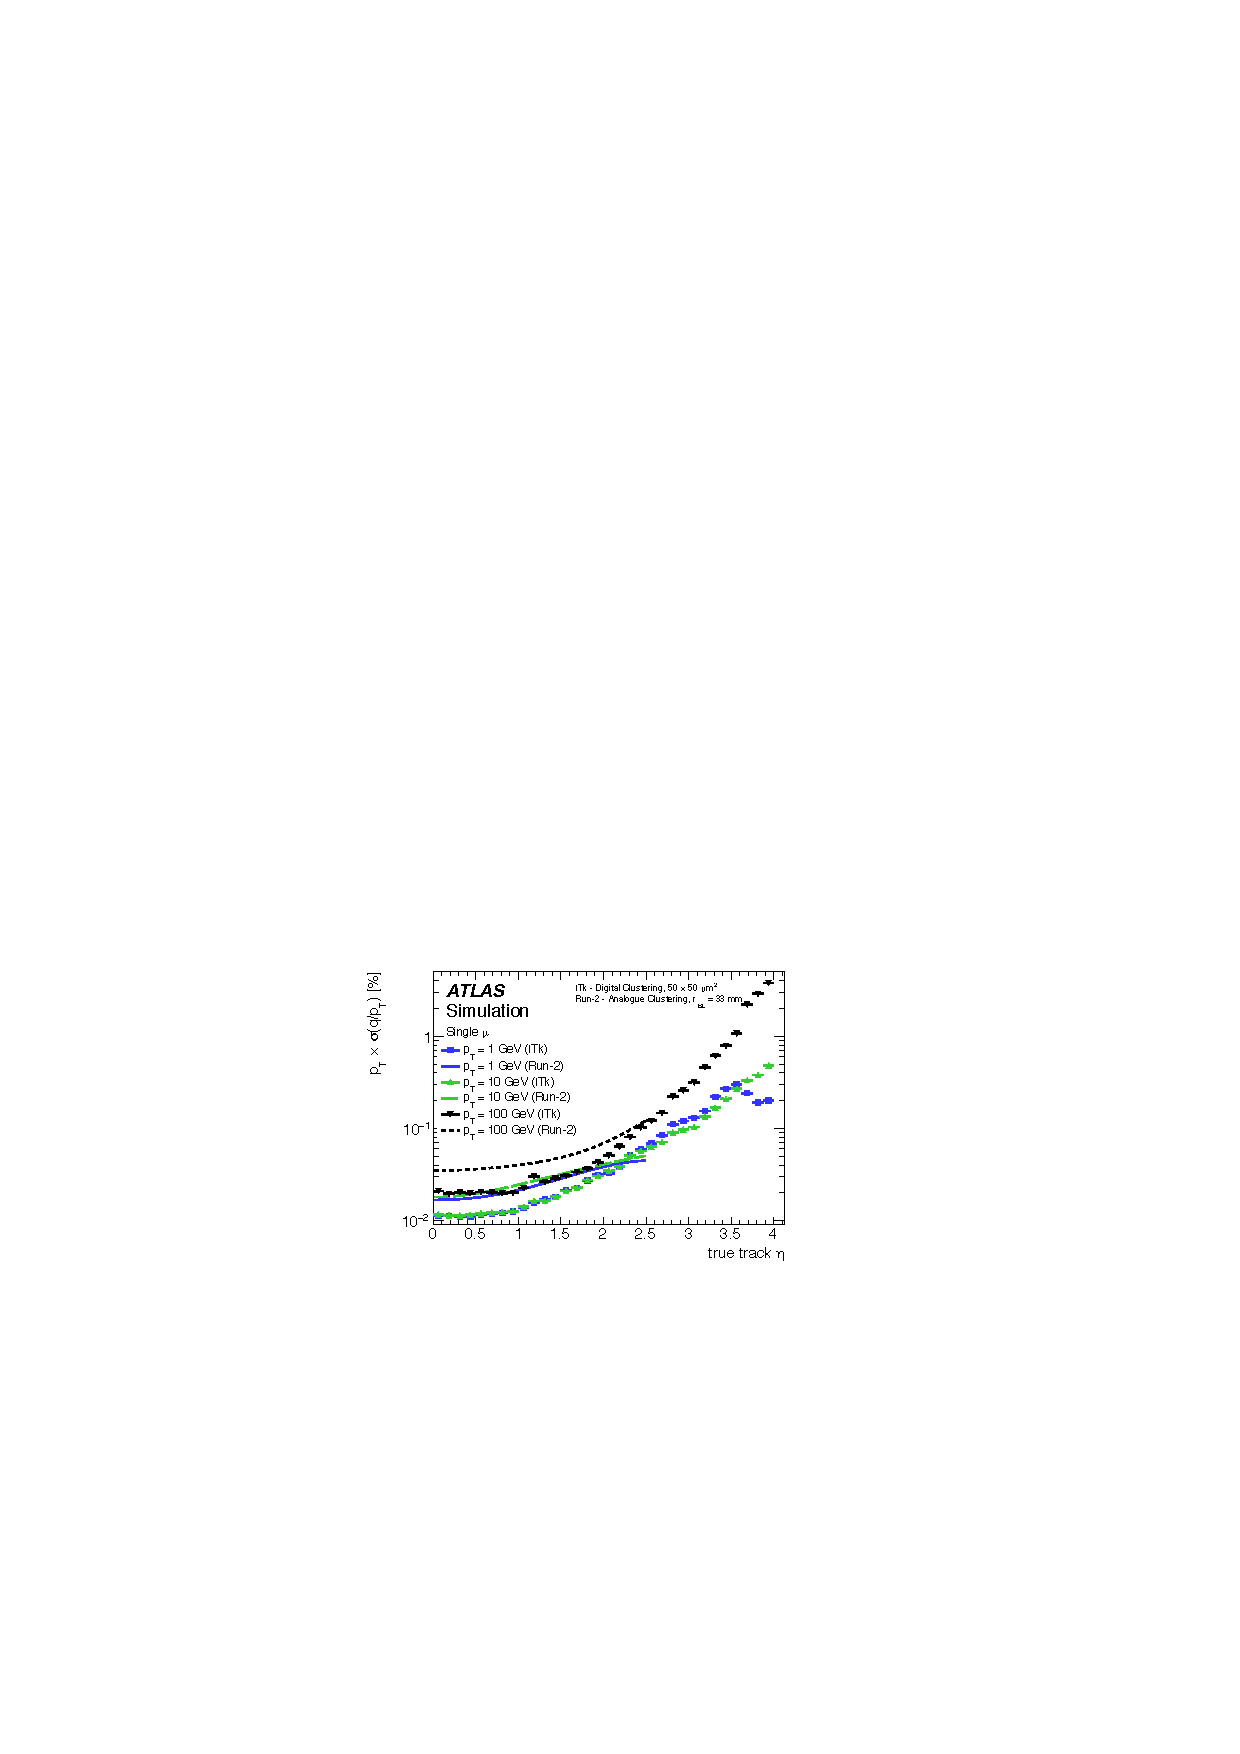
\includegraphics[width=0.47\textwidth]{figures/atlas-tdr-030-fig3-6e.pdf}
  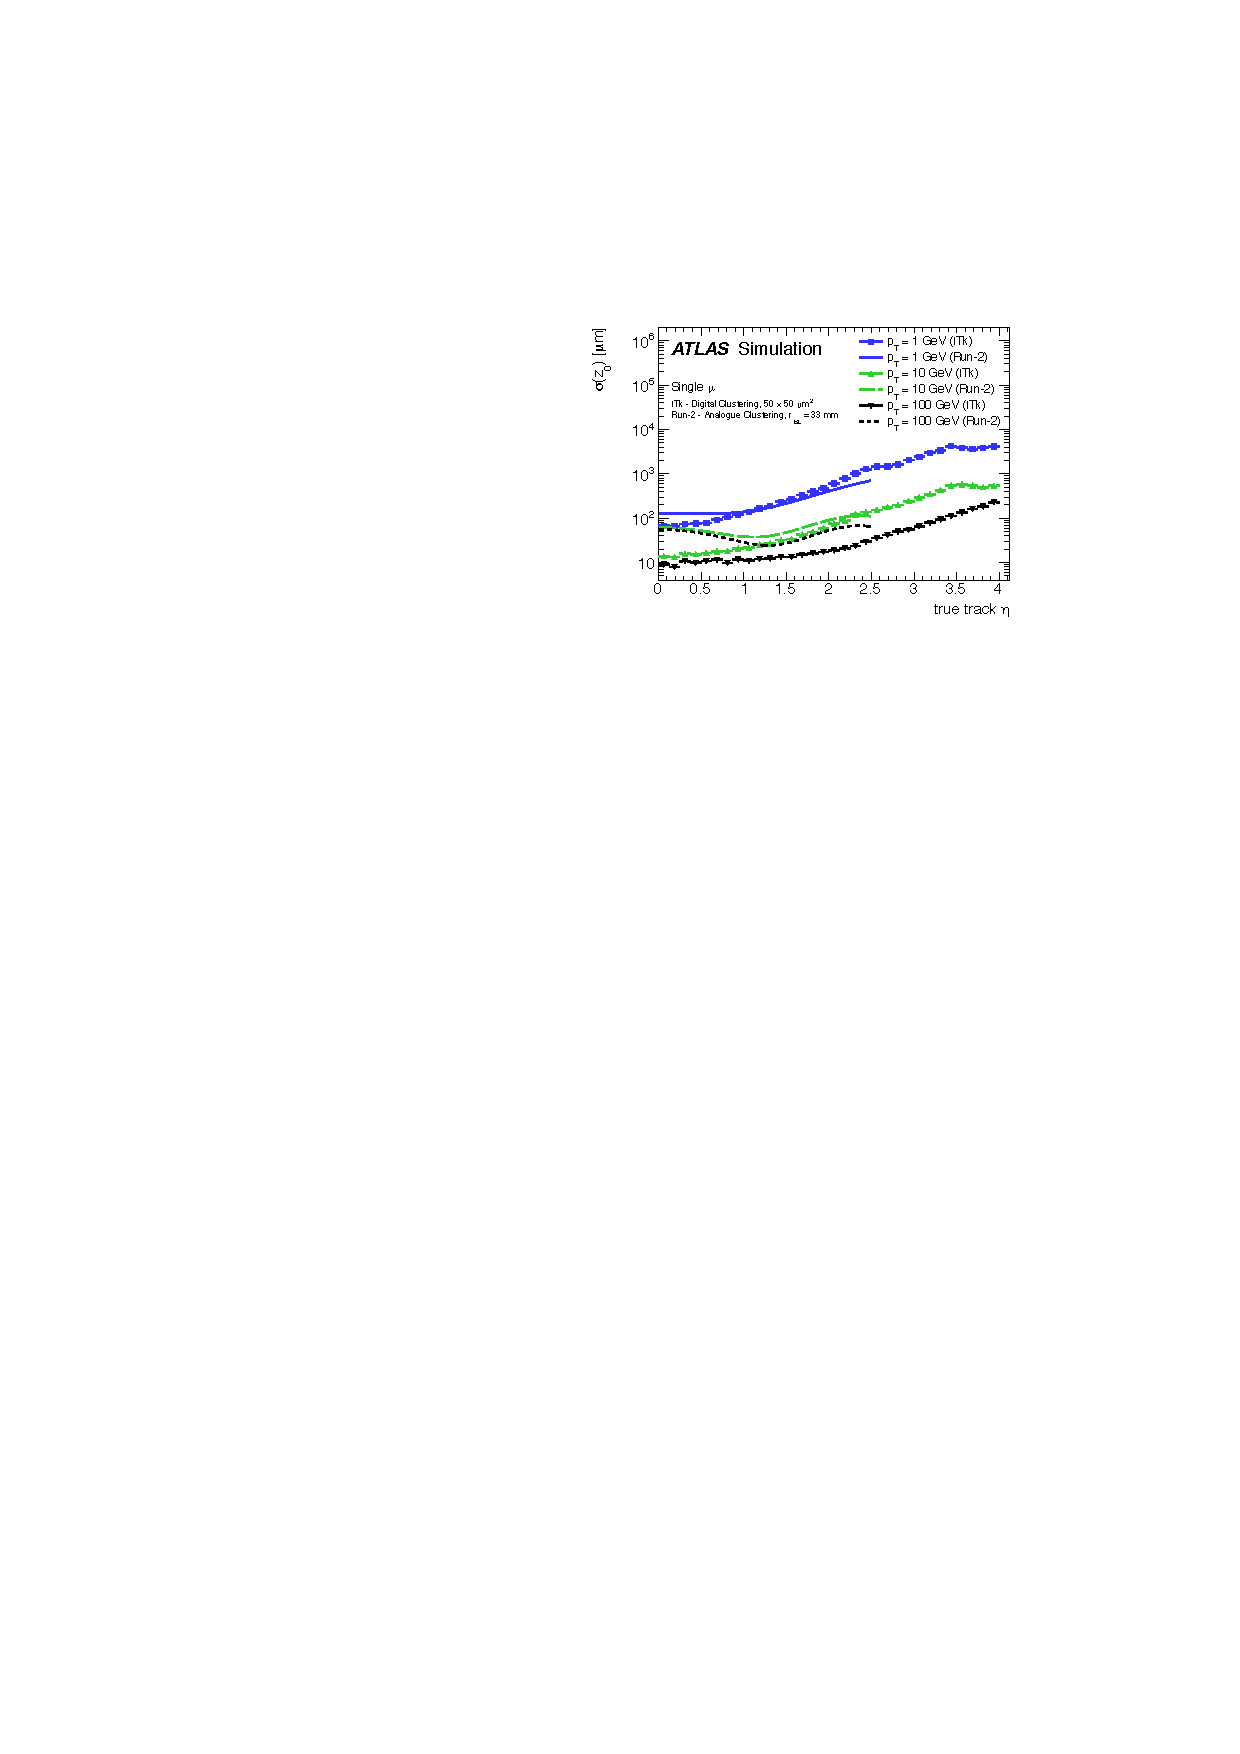
\includegraphics[width=0.47\textwidth]{figures/atlas-tdr-030-fig3-6b.pdf}
  \caption{Resolution of the transverse momentum (left) and longitudinal impact parameter (right) as a function of the pseudorapidity for the current (solid line) and the upgraded (points) ATLAS tracker~\cite{Collaboration:2285585}.}
  \label{fig:atlastrackres}
\end{center}
\end{figure}

\begin{figure}[t]
\begin{center}
  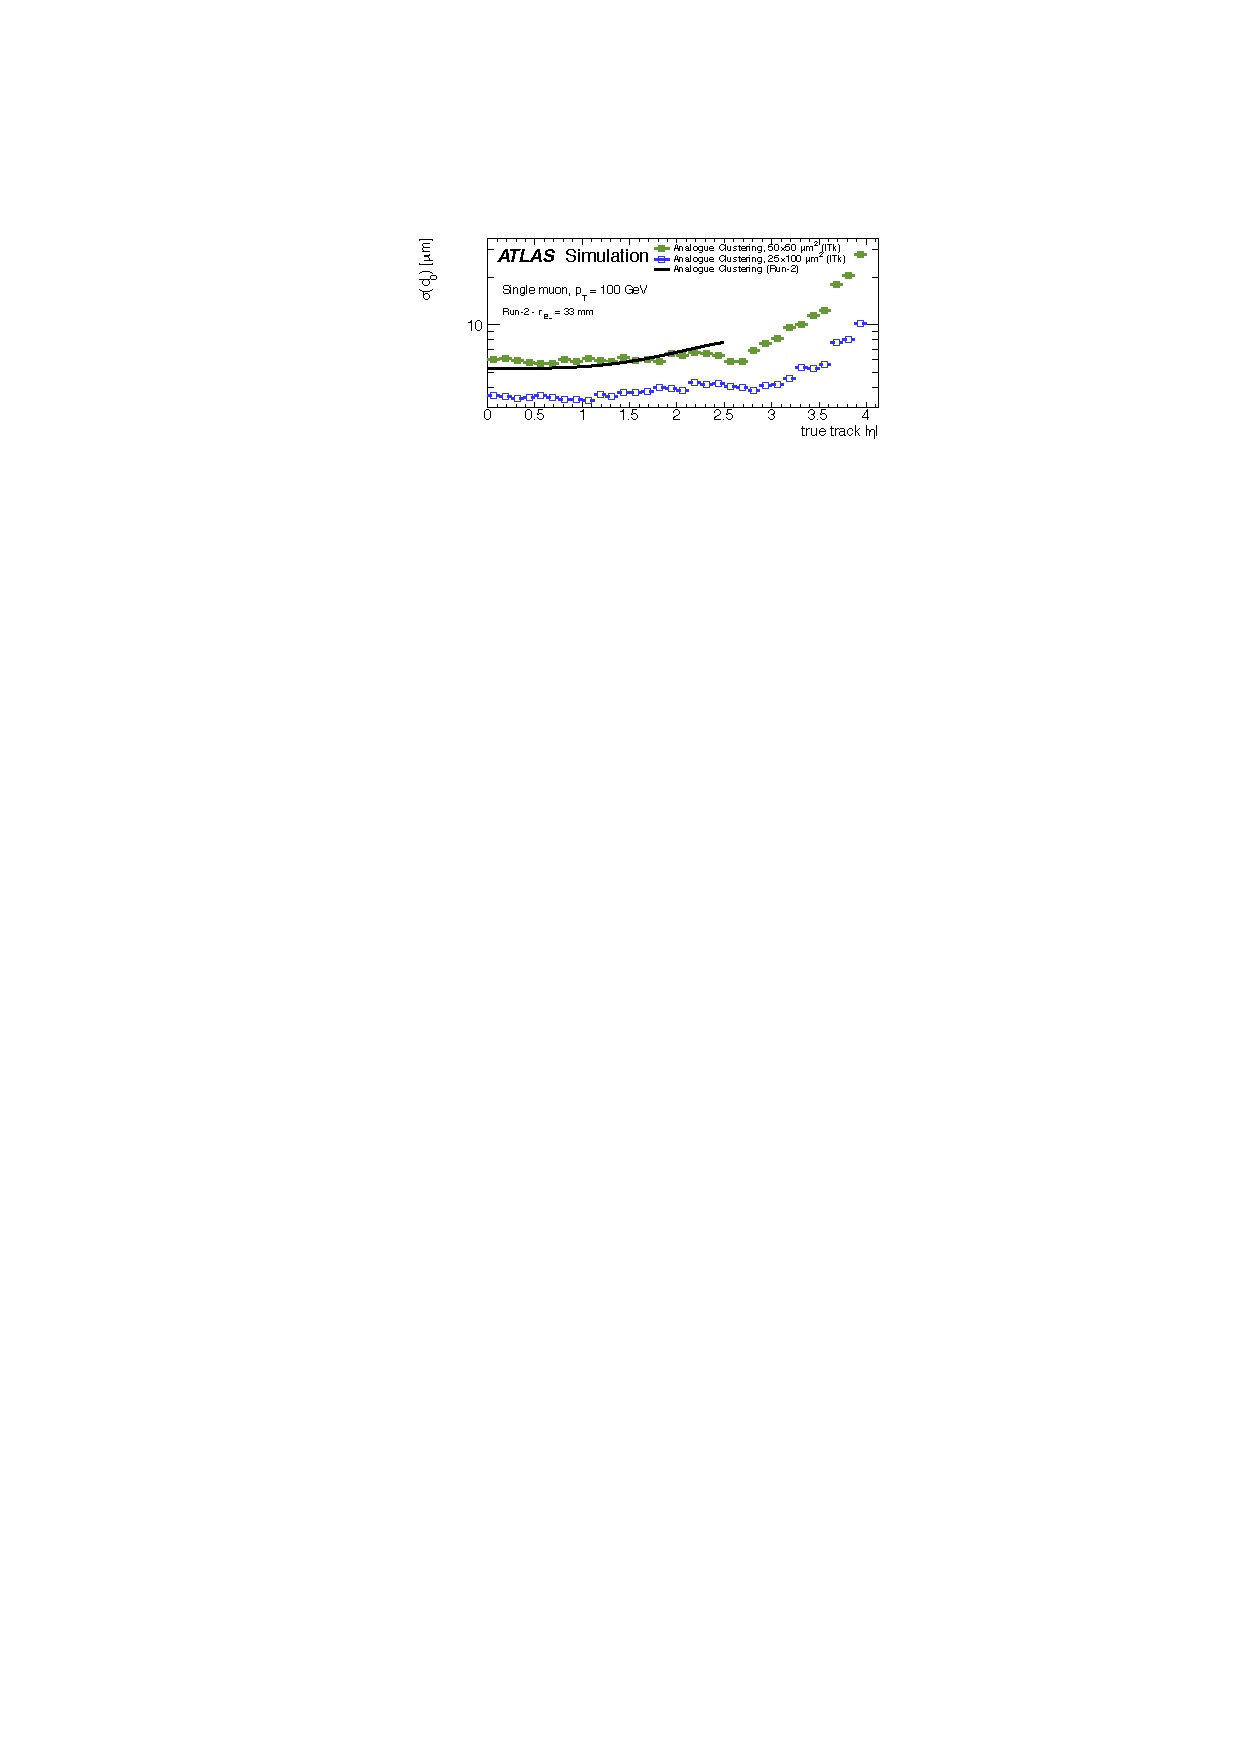
\includegraphics[width=0.9\textwidth]{figures/atlas-tdr-030-fig3-7a.pdf}\\
  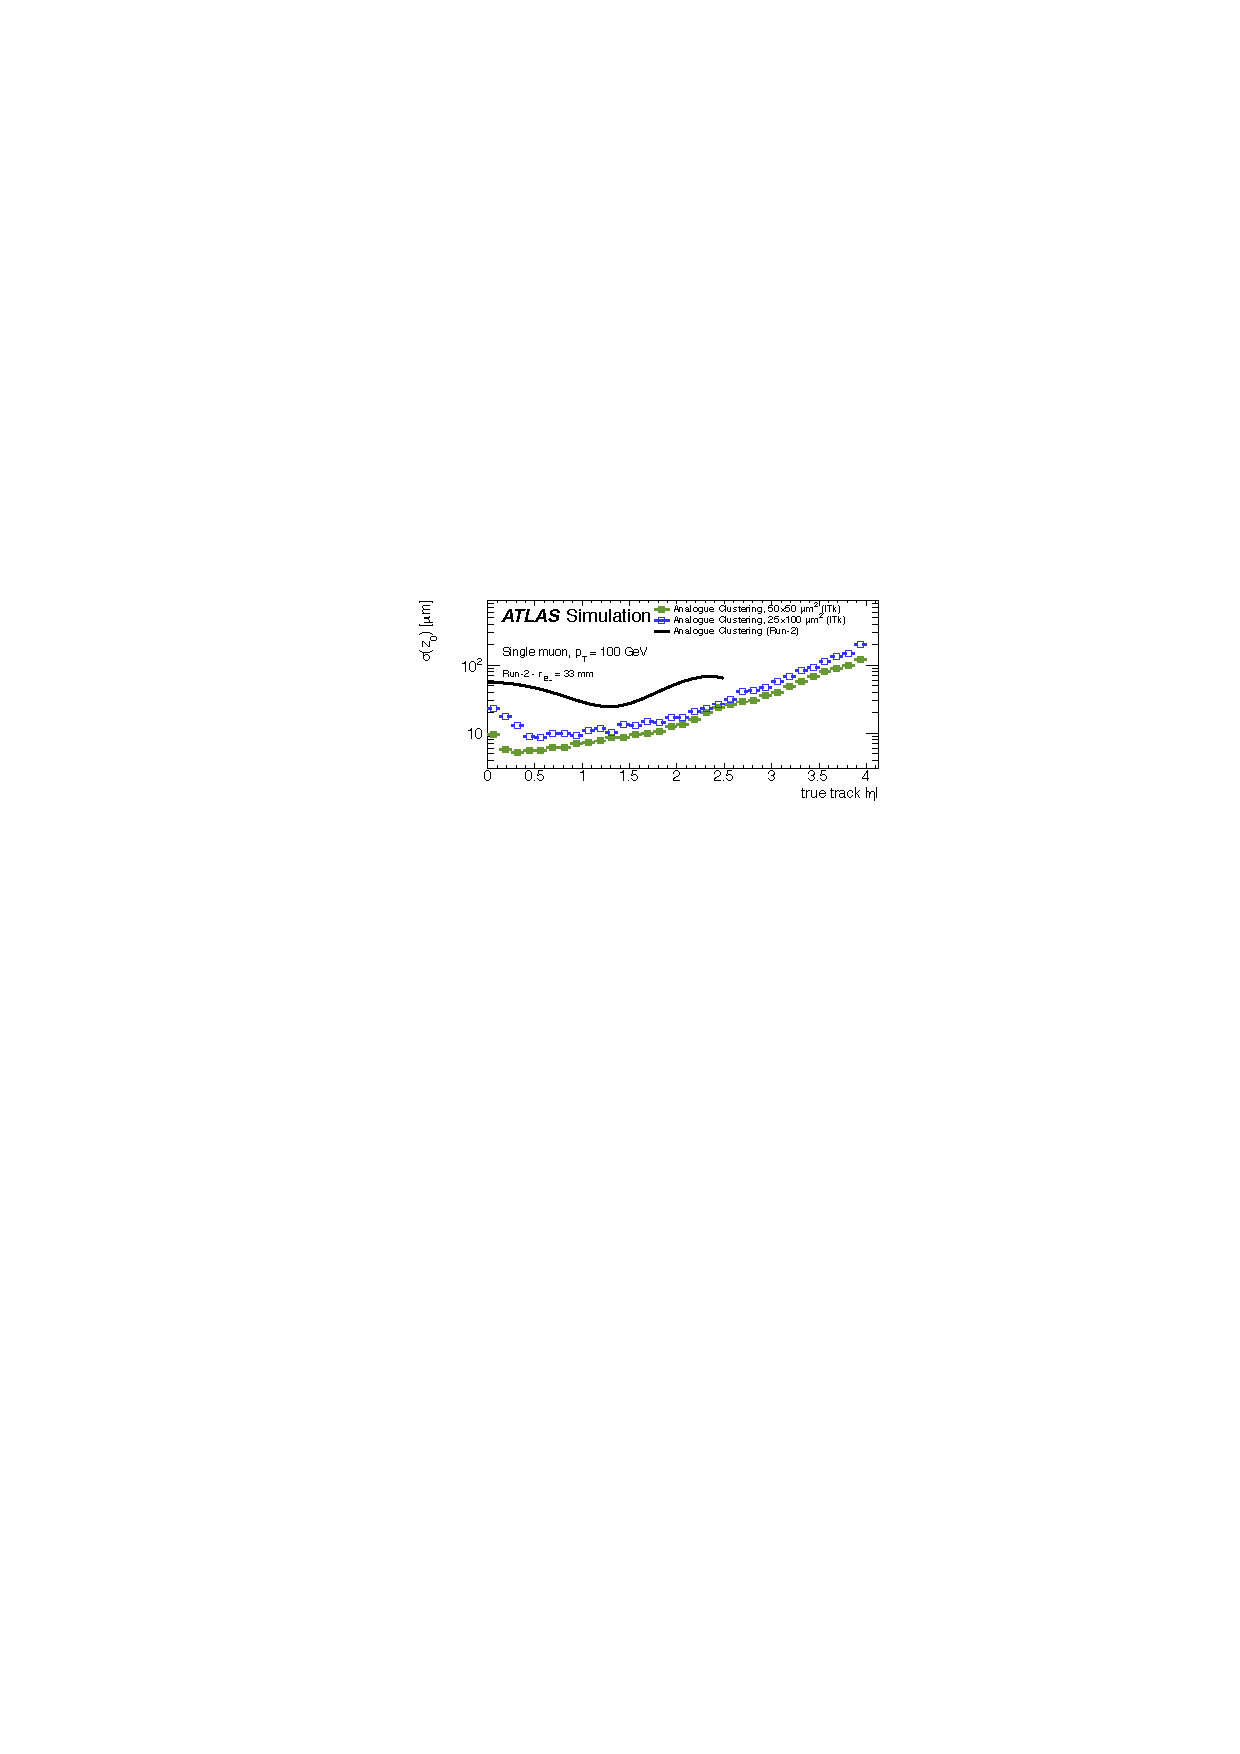
\includegraphics[width=0.9\textwidth]{figures/atlas-tdr-030-fig3-7b.pdf}
  \caption{Track parameter resolutions using analogue clustering for (left) transverse impact parameter; (right) longitudinal impact parameter. The resolutions are shown for single muons with $\pt=100$ GeV. The results of ITk are shown for $25\times100\,\,\mu\mathrm{m}^2$ and $50\times50\,\,\mu\mathrm{m}^2$ pixels, along with the current Run 2 detector performance~\cite{Collaboration:2285585}. }
  \label{fig:atlastrackanalog}
\end{center}
\end{figure}

\subsection{Upgrade Projection: LLP Searches} \label{sec:upgradesearch}

{\bf \textcolor{red}{[BS: Should we organize performance studied better?]}}

Searches for long-lived particles are well motivated by various classes of extensions of the Standard Model, discussed at length in Chapter~\ref{sec:motivated_theories}. Often, the production cross section for such processes is expected to be very small. The HL-LHC will allow for the collection of much larger data sets needed to reach better sensitivity to such BSM scenarios. The prospects are further strengthened with detector and trigger upgrades. This section discusses these potential improvements, and presents sensitivity projections on a number of benchmark LLP search channels with the aforementioned upgrades at the HL-LHC.

\subsubsection{Heavy Stable Charged Particles in CMS}

A number of new physics scenarios give rise to heavy stable charged particles (HSCPs) with long lifetimes that move with subrelativistical speed through the detector, heavily ionizing the sensor material as they pass through. In split SUSY models, the supersymmetric particles known as the stau ($\tilde{\tau}$) and the gluino ($\tilde{g}$) can have such characteristic signatures. The relevant simplified models are described in Sections~\ref{sec:EMcharge}--\ref{sec:coloredLLPs}, and current searches are described in Section~\ref{subsec:ExpHSCP}.

\paragraph{Sensitivity Projection with Tracker Upgrade}

Depending on the mass and charge of the new particles, HSCPs experience anomalously high energy losses through ionization ($dE/dx$) in the silicon sensors with respect to the typical energy losses of SM particles, as can be seen in Figure~\ref{fig:cmsupgrade_hscp} (left). At the CMS experiment, the current strip tracker features analog readout. Furthermore, the pixel detector featured analog readout during Phase 0 in 2016 and before, and currently features digital readout during Phase 1, which started at the beginning of the 2017 LHC run. Therefore, these detectors allow for excellent $dE/dx$ measurements.

At the HL-LHC, the upgraded CMS inner pixel detector will continue providing $dE/dx$ measurements, enabled by its time-over-threshold readout, while the outer tracker cannot provide such information, given that the readout is binary. To increase the sensitivity for signatures with anomalously high ionization loss, a second, programmable, threshold has been implemented in the short strip ASICs of the pixel-strip (PS) modules of the outer tracker, and a dedicated readout bit signals if a hit is above this second threshold.

Searches for HSCPs can thus be performed by measuring the energy loss in the inner pixel detector and by discriminating HSCPs from minimum ionizing particles based on the ``HIP flag'' in the outer tracker. The threshold of the minimum ionization needed to set the HIP flag is an adjustable parameter in each PS module independently. A threshold corresponding to the charge per unit length of 1.4 MIPs, resulting from preliminary optimization studies, is used in the simulation, and the gain in sensitivity obtained by using the HIP flag is studied.

An estimator of the degree of compatibility of the track with the MIP hypothesis is defined to separate candidate HSCPs from tracks from SM background sources. The high resolution $dE/dx$ measurements provided by the inner pixel modules are used for the computation of the $dE/dx$ discriminator. The tracks in background events have a low number of high threshold clusters with HIP flag, compared to those observed for tracks in HSCP signal events and slow-moving protons and kaons in minimum bias events.

In Figure~\ref{fig:cmsupgrade_hscp} (right), the performance of the discriminator is shown by evaluating the signal vs.~background efficiency curves to identify tracks from signal events and reject those originating from backgrounds. The performance curves are evaluated for two different strategies for the discriminator: the $dE/dx$ discriminator, which relies solely on the inner pixel modules ($dE/dx$-only, ignoring the HIP flags), and a recomputed discriminator which includes the HIP flags from the outer tracker PS modules ($dE/dx$ + HIP flags). The signal versus background efficiency performance curves demonstrate that for a background efficiency of $10^{-6}$, analogous to the current analysis performance, the $dE/dx+$HIP-based discriminator leads to an expected signal efficiency of $40\%$, around 4 to 8 times better than the $dE/dx$-only discriminator. In the $dE/dx$-only scenario, the efficiency for the HSCP signal is about 8 times smaller than that obtained in current data. The inclusion of the HIP flag for the PS modules of the Outer Tracker restores much of the efficiency, so that the same sensitivity as in Phase 1 will be realized with about four times the luminosity of Phase 1. The Phase 1 sensitivity will be surpassed with the full expected integrated luminosity of the HL-LHC. This study demonstrates the critical impact of the HIP flag in restoring the sensitivity of the CMS tracker for searches for highly ionizing particles in the HL-LHC era.

Additionally, the current CMS inner pixel detector provides measurements of charge deposits in each pixel up to $9,600$ electrons over a range of $4$-bits in the digitizer. While it may be difficult to increase the number of bits used to store the charge information due to data rate constraints, it is possible to adopt a dual-slope mapping from charge deposit to ADC counts in the digitizer, which will preserve the granularity for lower charge deposits, while giving more information for highly ionizing particles such as HSCPs. This option is currently being studied to evaluate the potential improvement to $dE/dx$ measurements. Furthermore, tuning of the HIP flag threshold may bring additional improvements.

\begin{figure}[t]
\begin{center}
  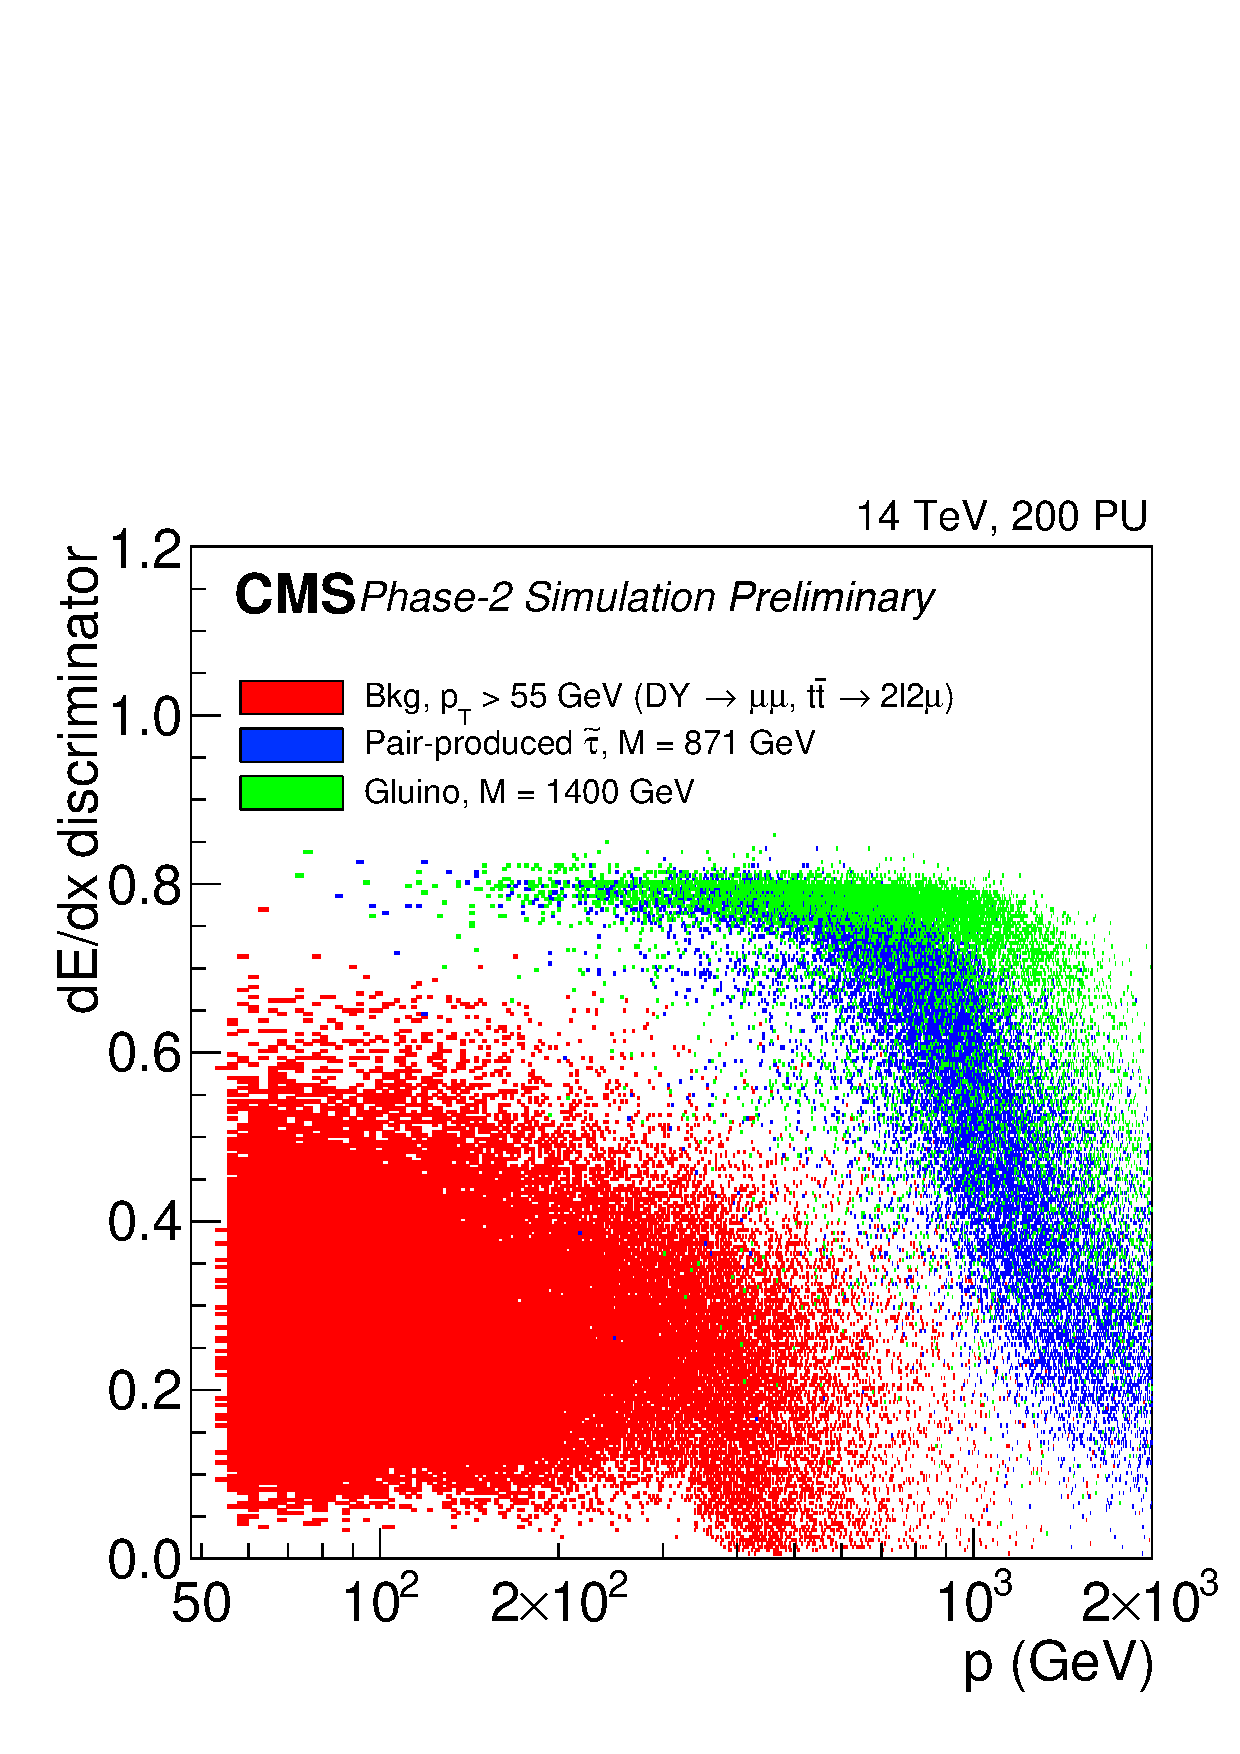
\includegraphics[width=0.47\textwidth]{figures/HSCP/TDR-17-001_fig6_26_a_HSCP_SpecialPlot_v2.pdf} \hfill
  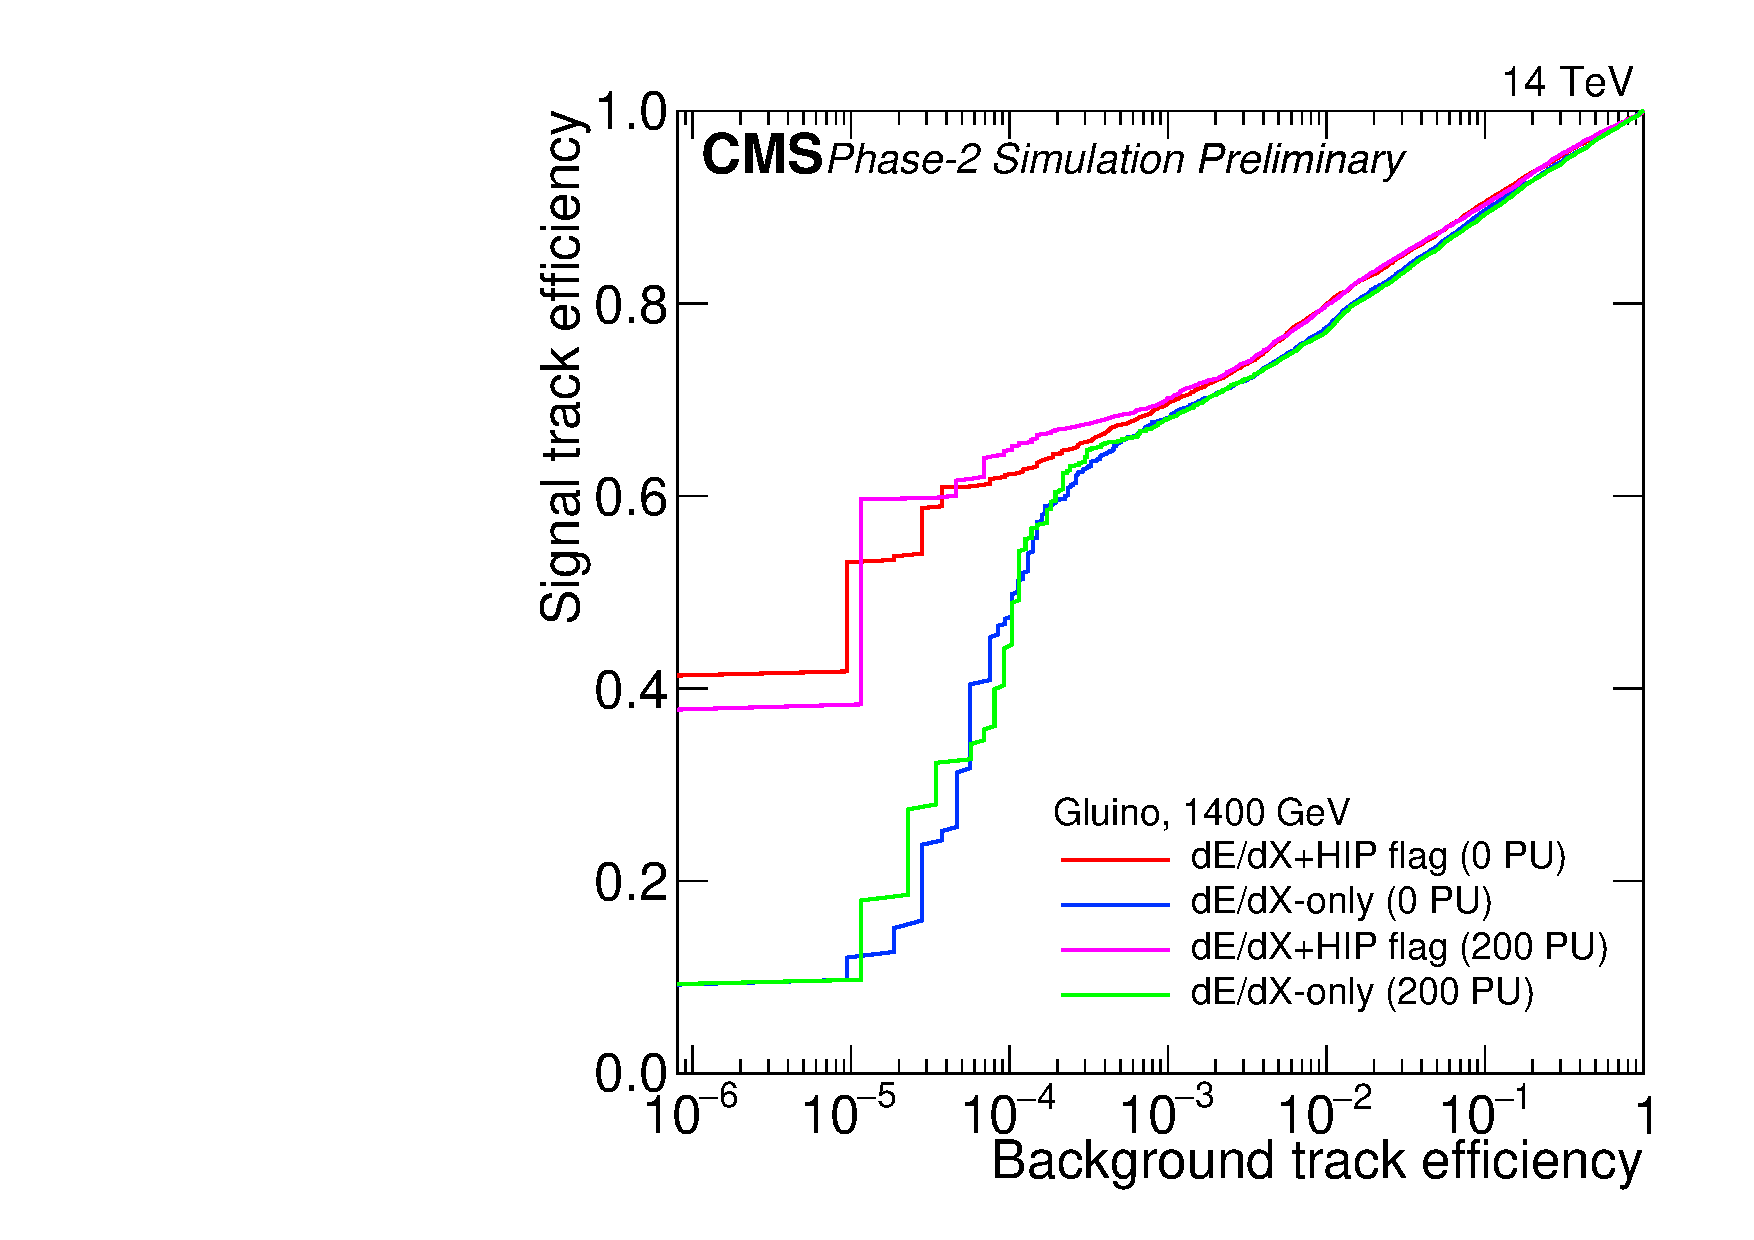
\includegraphics[width=0.47\textwidth]{figures/HSCP/TDR-17-001_fig6_27_a_HSCP_Comparison_ROC_Gluino_M1400_NoPU_Super_v2.pdf}
  \caption{{\bf Left:}~distribution in CMS of the $dE/dx$ discriminator versus track momentum ($p$) for tracks with high momentum ($\pt > 55$~GeV) in background events (red) and for candidate signal particles. Pair produced $\tilde{\tau}_S$ with a mass of 871~GeV (blue), and a gluino with a mass of 1400~GeV (green), are shown. {\bf Right:}~the performance of the $dE/dx$ discriminator for selecting gluinos in events at rates of 0 pile-up (PU) and 200 PU. The signal vs. background efficiency performance curves for a discriminator making use of both the pixel information and the outer tracker HIP flag (red and magenta) demonstrate a better performance compared to a discriminator trained to exploit only the $dE/dx$ information from the pixel modules (blue and green), for a background rejection of $10^{-6}$~\cite{Collaboration:2272264}.}
  \label{fig:cmsupgrade_hscp}
\end{center}
\end{figure}

\paragraph{HSCP Trigger with Muon Detector Upgrade}

The upgrade of the RPC system will allow the trigger and identification of slowly moving particles by measuring their time of flight to each RPC station with a resolution of $\mathcal{O}(1)$~ns. The new RPC detectors have a two-end strip readout, which provides precise measurements of the hit position in the local $y$ or the global $\eta$ coordinate. The speed of muon-like particles and the time (bunch crossing) of their origin will be computed with a fast algorithm to be implemented in the Level-1 trigger at the HL-LHC.

The RPC detectors are synchronized to register muons moving at the speed of light with a local time equal to zero with respect to the collision event that produced the trigger. Slow-moving particles, as HSCPs, will arrive with a delay depending on their speed as shown in Figure~\ref{fig:hscp_time}. This time delay, measured by each RPC layer crossed by the HSCP, is exploited in order to trigger on and reconstruct such particles.

\begin{figure}[t]
\begin{center}
  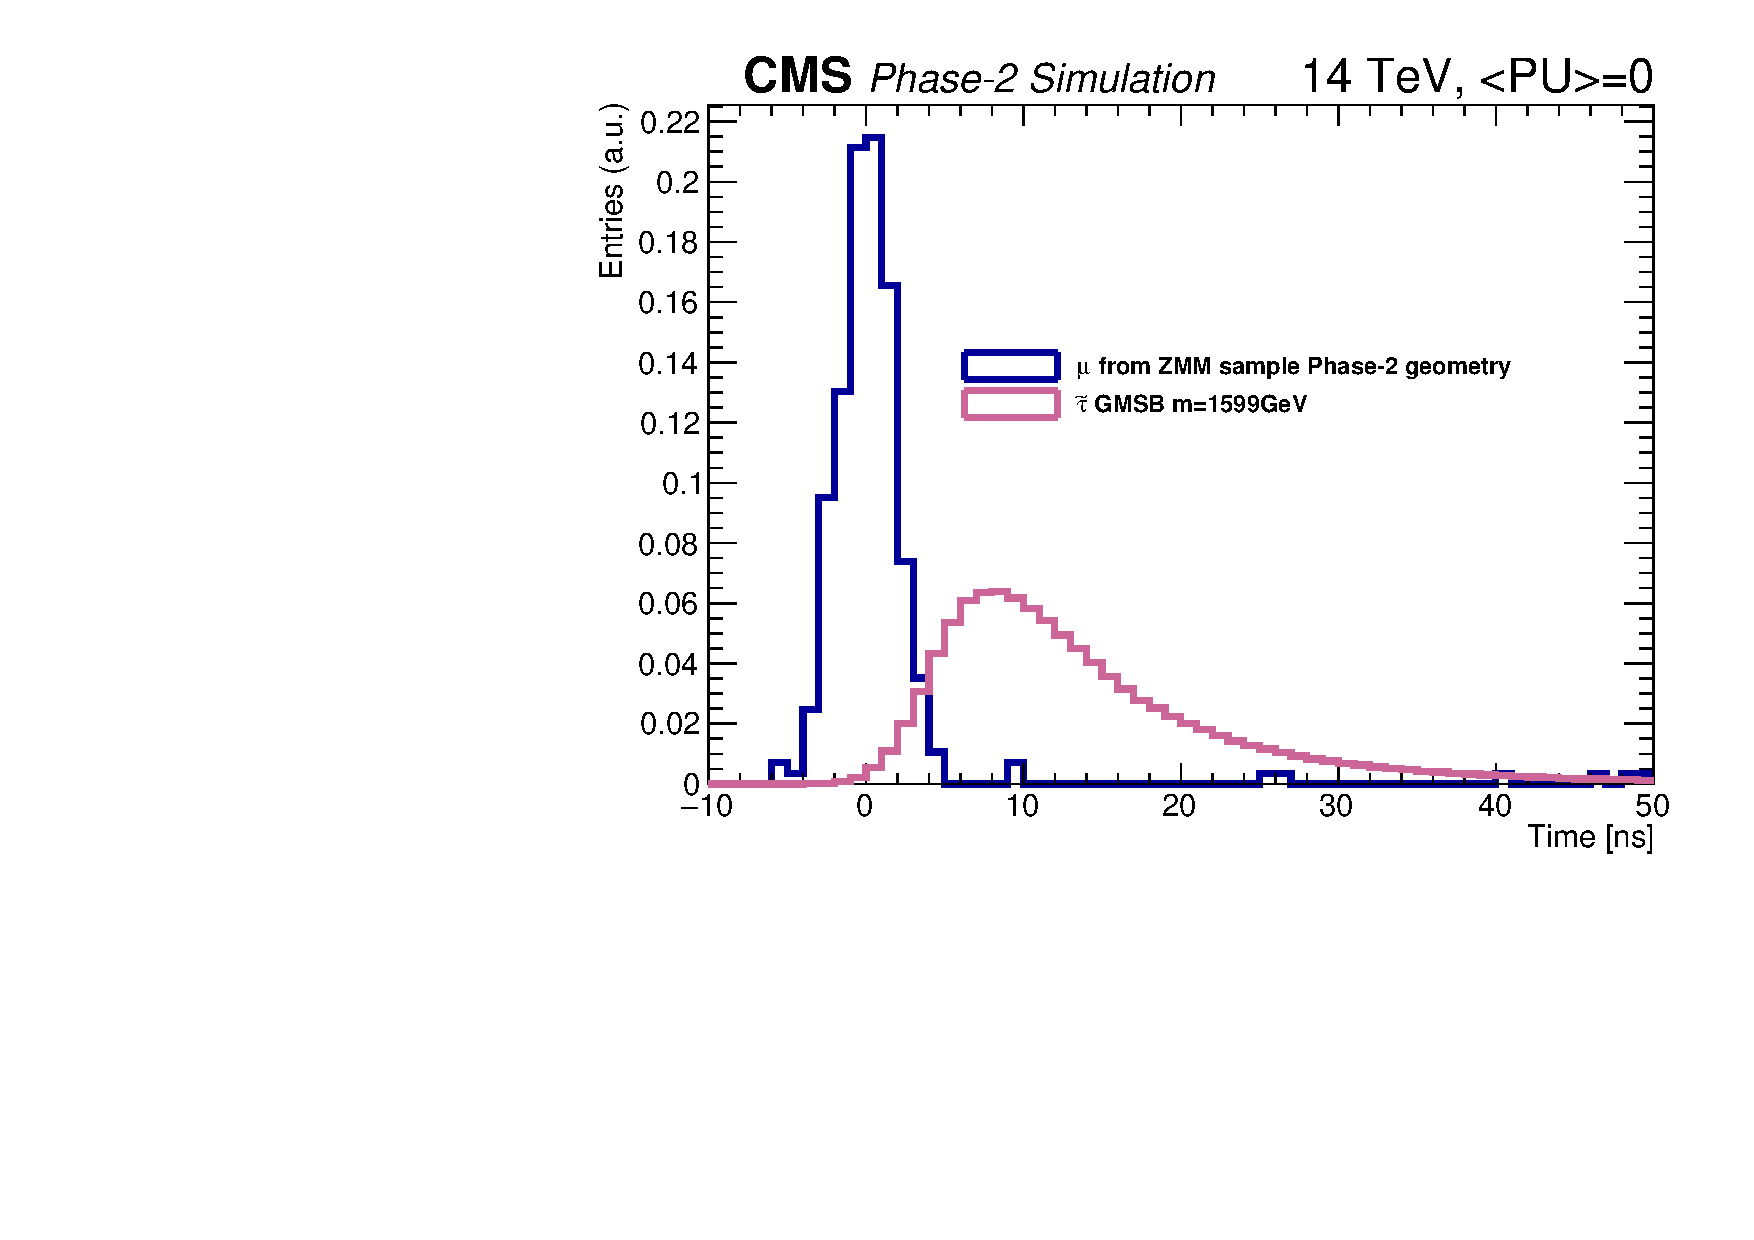
\includegraphics[width=0.9\textwidth]{figures/HSCP/time.pdf}
  \caption{RPC hit time measurement distribution in CMS for muons from $Z \to \mu\mu$ events and for semi-stable $\tilde \tau$ particles with m$\approx$1600~GeV, produced in $pp \to \tilde \tau \tilde \tau$ processes~\cite{Lourenco:2283189}.}
  \label{fig:hscp_time}
\end{center}
\end{figure}

The principles of the proposed HSCP trigger algorithm are illustrated in Figure~\ref{fig:HSCP_diagram}. In this figure, the vertical axis is the time of signals measured in RPC chambers, as synchronized so that muons moving nearly at the speed of light from a particular collision are measured at the time of the collision. The horizontal axis is the distance from the collision point to the position of the RPC at which the time is measured. The diagram shows three successive bunch crossings, two of which contain muons represented at horizontal lines. The diagram also shows the RPC time measurements from two HSCPs having slopes different from zero due to their traveling significantly slower than the speed of light. The time delay $\Delta t$ is related to the speed $v$ of an HSCP via the following equation:
%
\begin{equation}
\label{eq:HSCP_delay}
\Delta t = d\left(\frac{1}{v}-\frac{1}{c}\right).
\end{equation}
%
Here $d$ is the distance between the interaction point (IP) and the point where an HSCP crosses an RPC. For RE4/1 chambers and $\beta = v/c = 0.2$, the delay time is $>6$ bunch crossings, comparable to $150 \, \mathrm{ns}$.

\begin{figure}[t]
  \centering
  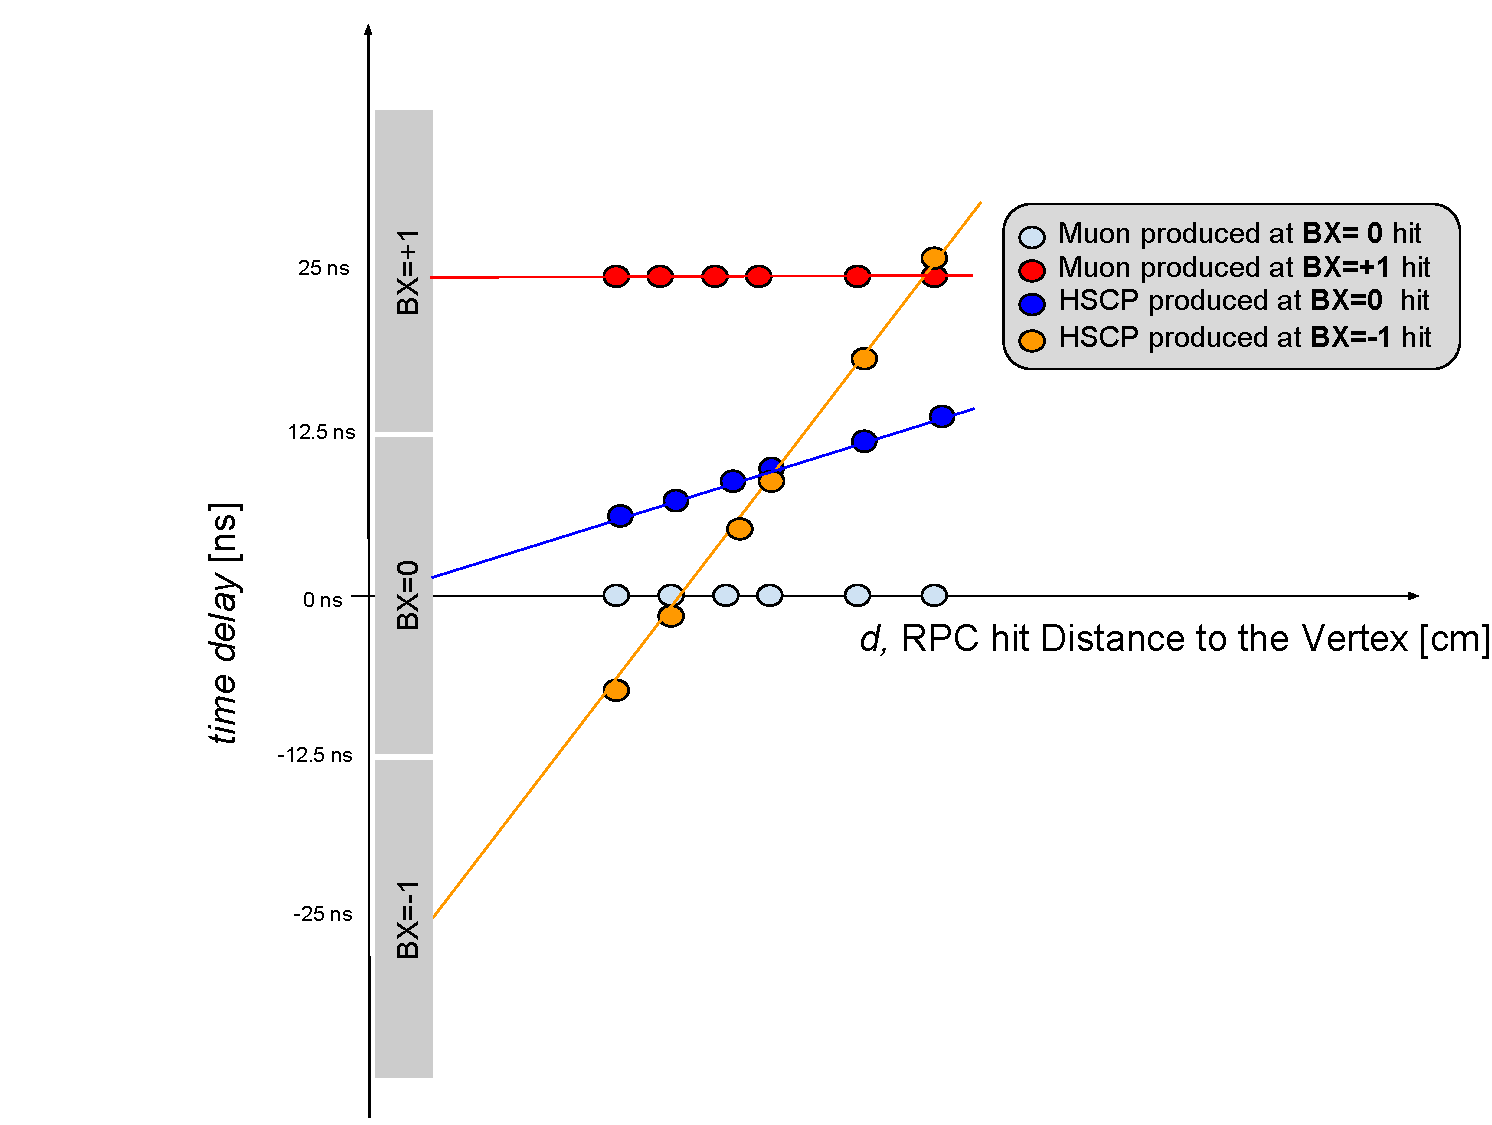
\includegraphics[width=0.9\textwidth]{figures/HSCP/diagram.pdf}
  \caption{Diagram showing times measured at different RPC stations for particles originating at different bunch crossings and with different velocities in CMS. The $x$-axis represents the distances from IP to RPC detectors, while the $y$-axis corresponds to time. The clock at each RPC station is tuned so that particles moving with the speed of light are registered with the exact same ``local'' times. Hence, relativistic particles are represented by horizontal lines on this diagram~\cite{Lourenco:2283189}.}
  \label{fig:HSCP_diagram}
\end{figure}

A penetrating charged particle leaves a trail of hits in RPC chambers along its trajectory. The time of flight can be computed in each RPC station with respect to a number of bunch crossing hypotheses. Should there be a common velocity solution, derived from Eq.~(\ref{eq:HSCP_delay}), with $\beta < 0.6$, a trigger is formed. For $\beta >0.6$, the delays are small and can be handled by the Phase 1 trigger. The performance of this algorithm has been studied with the CMS full simulation. All the detector effects (e.g., electronics jitter, signal time propagation along strips) are considered. A particle-speed measurement resolution is shown in Figure~\ref{fig:HCP_Trigger} (right) for the case of 25~ns signal sampling time (Phase 1) and 1.56~ns sampling time provided with the upgraded RPC Link Board System. For both plots, an HSCP signal is shown.

\begin{figure}[t]
\begin{center}
  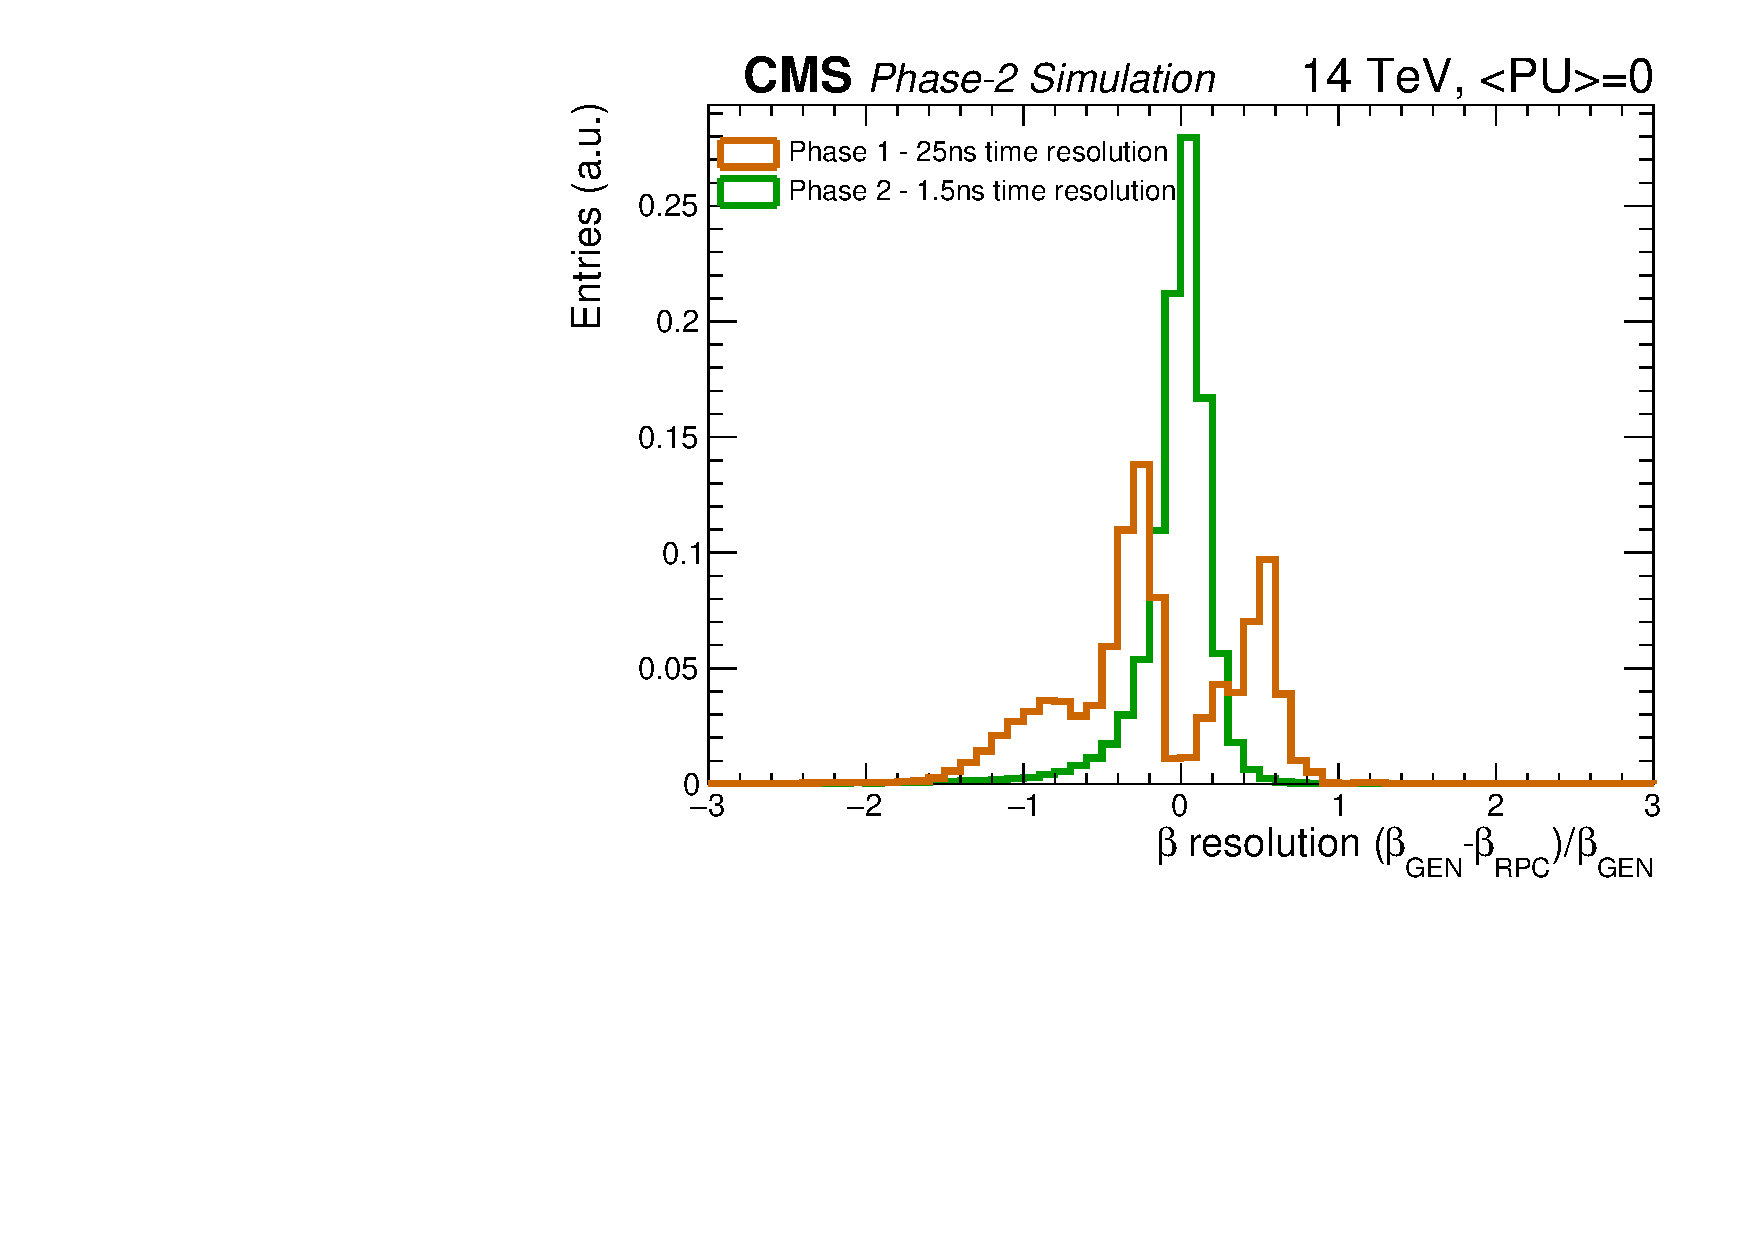
\includegraphics[width=0.47\textwidth]{figures/HSCP/beta_GenRes_2.pdf} \hfill
  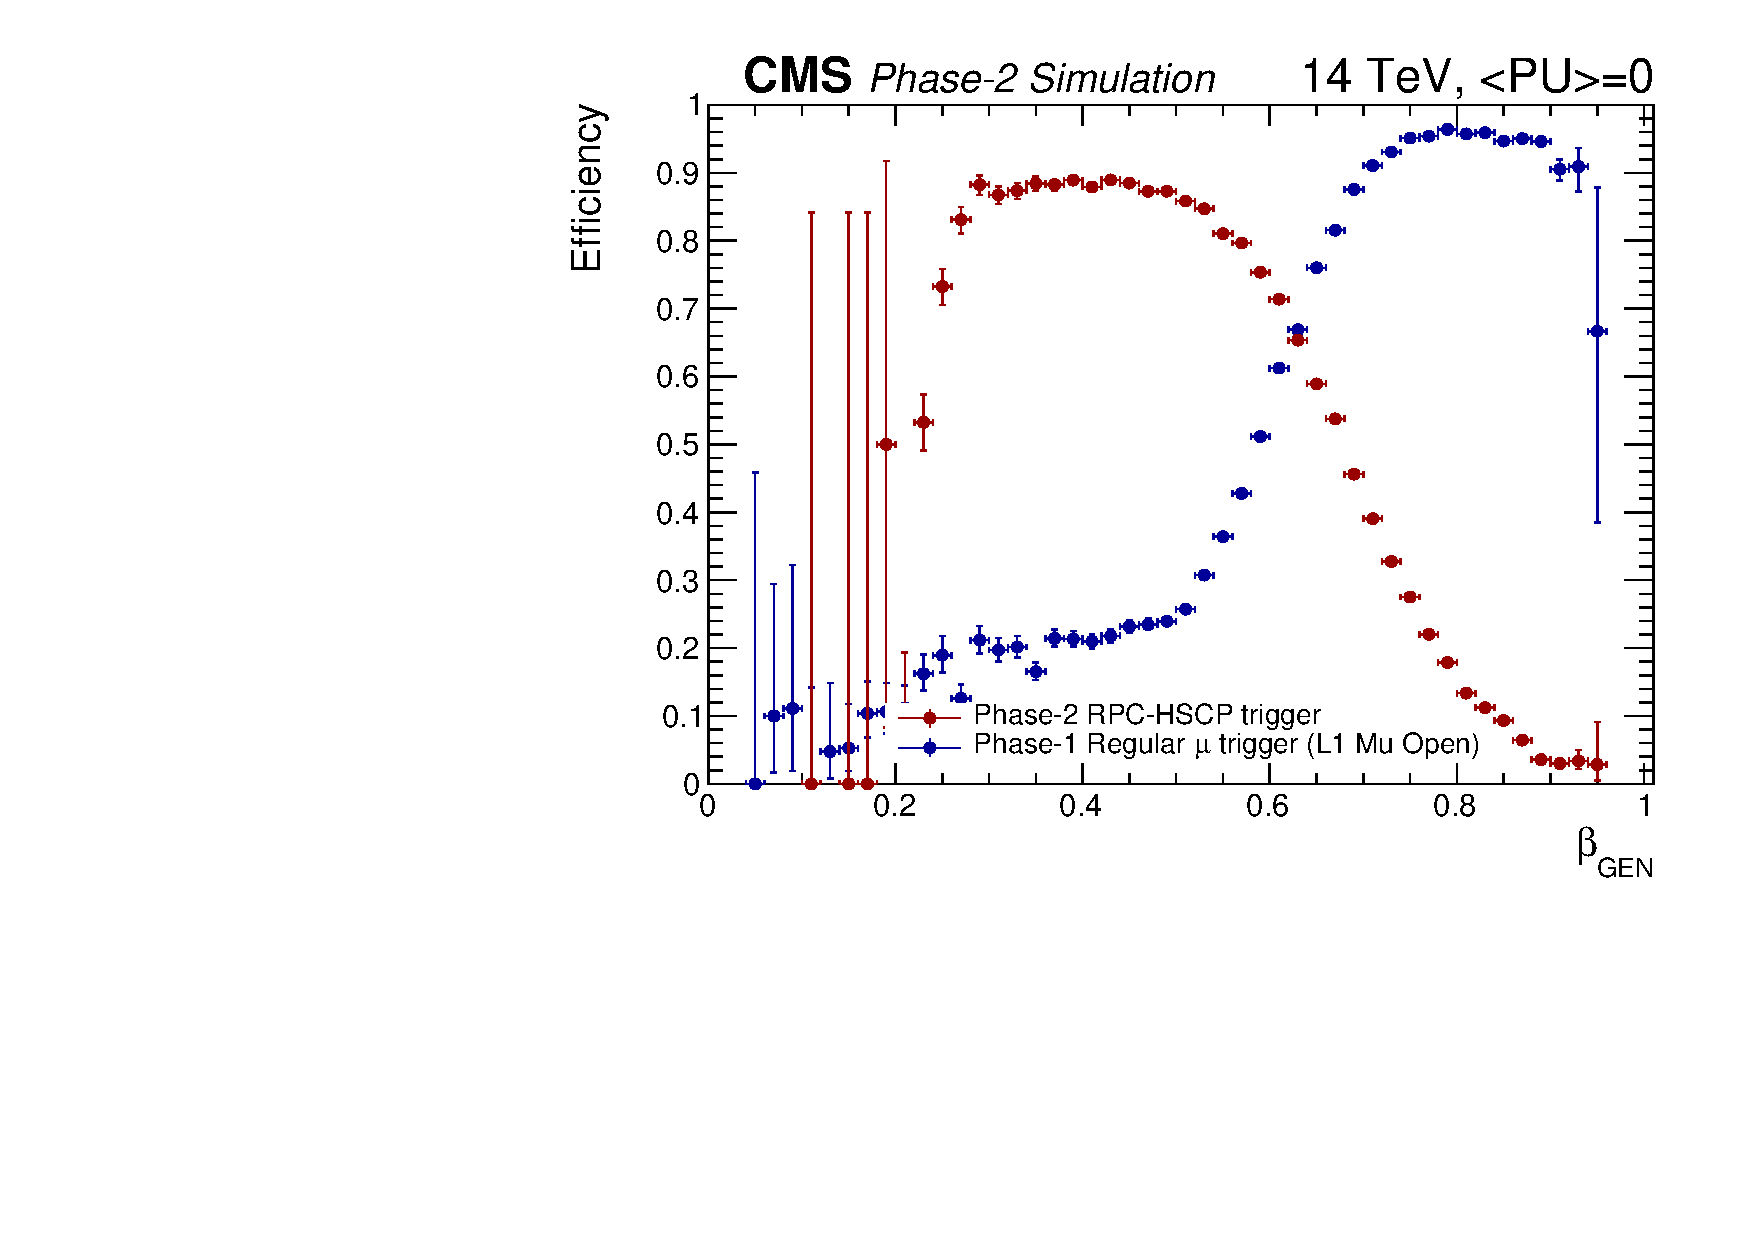
\includegraphics[width=0.47\textwidth]{figures/HSCP/trigEff-Mu-HSCPTriggers.pdf}
  \caption{{\bf Left:}~resolution of a particle-speed measurement at L1 trigger with Phase 1 and upgraded RPC Link Board System. {\bf Right:}~the efficiency as a function of $\beta$ of the standard L1 muon trigger without any $\pt$ threshold, and the RPC-HSCP Phase 2 trigger with $1.56$~ns sampling time. For both plots, an HSCP signal is shown~\cite{Lourenco:2283189}.}
  \label{fig:HCP_Trigger}
\end{center}
\end{figure}

The efficiency of the RPC-HSCP algorithm as a function of $\beta$ is studied and compared with the standard L1 muon trigger. The results are shown in Figure~\ref{fig:HCP_Trigger} (right). The current CMS-HSCP Phase 1 trigger performs well down to $\beta \approx 0.75$. The upgraded RPC Link Board System will allow for the triggering, at the
correct bunch crossing, on possible HSCPs with velocities as low as $\beta \sim 0.25$.

Possible improvements for this trigger proposal in the $\beta$ measurement could be achieved by matching tracks in the track trigger to the HSCP muon trigger.

\subsubsection{Displaced Muons in CMS}


Many BSM theories predict particle decays with displaced muon or muon pairs in its final state, such as dark SUSY and GMSB with smuons.
In order to demonstrate the physics potential of displaced muons at the HL-LHC with the CMS detector,
a particular SUSY model is selected where the displaced signature consists of a dimuon final state emerging from the decay of heavy sparticles (smuons).
Searches for the direct production of heavy sparticles with long lifetimes are difficult in the present LHC runs,
owing to small cross sections and limited integrated luminosity, and will only become possible at the HL-LHC.

In gauge-mediated SUSY breaking models, smuons can be (co-)NLSPs (next to lightest supersymmetric particles) and decay to a muon and a gravitino~\cite{Ruderman:2010kj}.
When the slepton is long lived, the final state signature is two displaced oppositely charged muons and significant missing transverse energy.
The smuon pair production has the advantage that it can be characterized by a very clean final state topology, and
we will therefore focus on the process $q \bar q \to \widetilde{\mu} \widetilde{\mu}$, where the two smuons decay far from the primary interaction vertex.
For this process, the muon $|d_0|$ can reach up to approximately one meter (or longer) for sufficiently large lifetimes,
as shown in Figure~\ref{fig:perfDisplaced} (left). Figure~\ref{fig:perfDisplaced} (right)
compares the number of hits created by these displaced muons in the CMS muon system in Phase 2 and the current CMS detector.
The hits plotted here are those associated with the displaced stand-alone muon tracks, which is a muon track reconstruction
algorithm specifically designed for displaced muons that can only be reconstructed in the muon system~\cite{CMS-DP-2015-015}.


\begin{figure}[t]\begin{center}
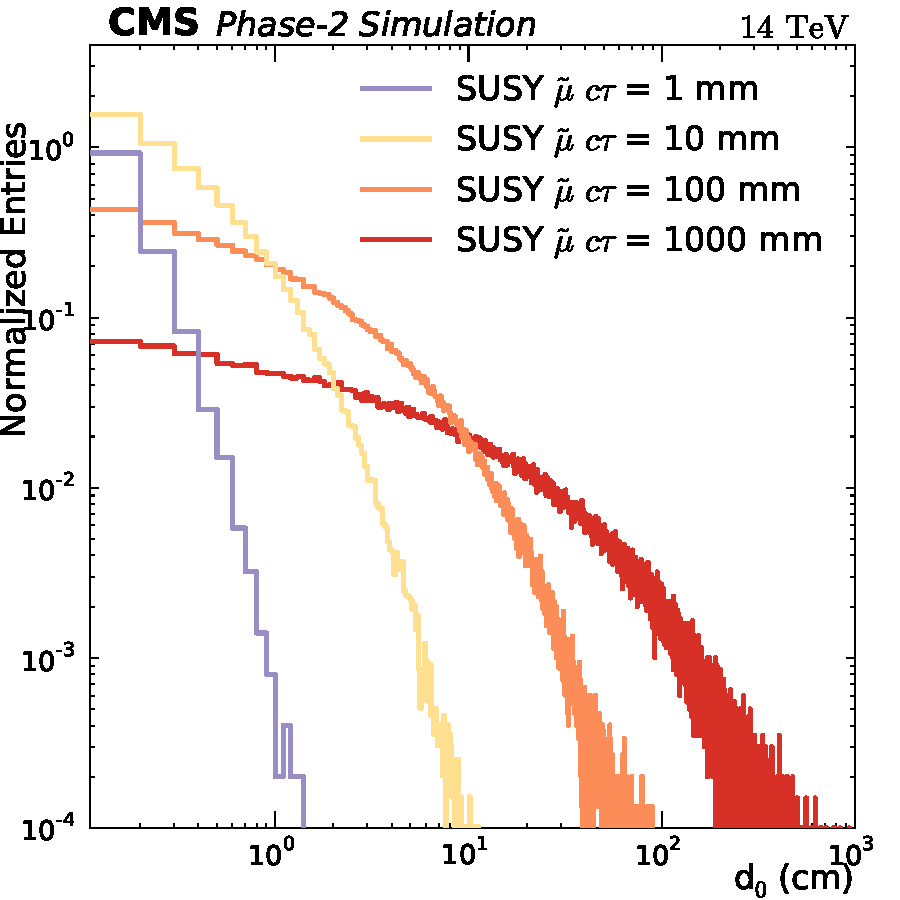
\includegraphics[width=0.47\textwidth]{figures/Stage0h1_0_d0_smuon_daughter}
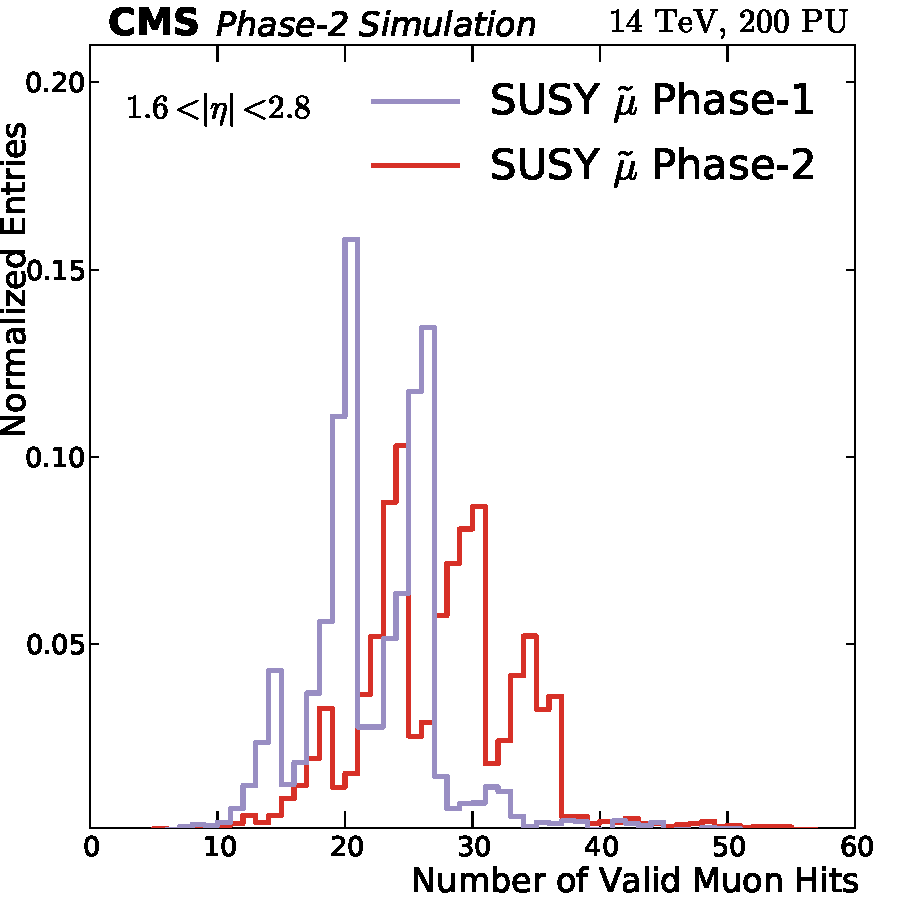
\includegraphics[width=0.47\textwidth]{figures/MuonHitsEndcap}
\caption{
{\bf Left:} the muon transverse impact parameter, $|d_{0}|$, for several simulated smuon decay lengths, $c\tau$, at the generator level.
{\bf Right:} distribution of the minimum number of valid hits in the CMS Phase 2 muon system for a SUSY $\widetilde{\mu}$ with $m_{\widetilde{\mu}}$ = 500~GeV and $\tau$ = 1000~mm for the Run 2 (blue) and Phase 2 (red) detectors~\cite{Lourenco:2283189}.
}
\label{fig:perfDisplaced}
\end{center}
\end{figure}

Standard triggers and reconstruction algorithms that use the position of the primary vertex will not efficiently reconstruct tracks with large impact parameters. Consequently, triggering on and reconstructing muons produced far  from the IP is challenging and requires dedicated triggers and reconstruction algorithms. The upgrades to the muon system in CMS, as well as the L1 tracking capabilities, significantly improve the experiment's ability to search for displaced muons at the HL-LHC.

\paragraph{Triggering on Displaced Muons}

The momentum resolution of the L1 muon trigger for muons coming from the primary vertex will be greatly improved by adding information from the L1 track trigger, discussed previously. The L1 track trigger can also be directly combined with trigger primitives at the first stage of the muon track-finder electronics; this would mirror the offline reconstruction of ``Tracker Muons'' which improve the efficiency for very low-$\pt$ muons, especially in the barrel region.

To trigger on both prompt and non-prompt muons effectively at L1, a stand-alone L1 muon generates two $\pt$ measurements for each muon, prompt and non-prompt, which are matched with L1 tracks. If the track match is successful, the L1 track trigger $\pt$ is used and a prompt candidate is formed. If the match is unsuccessful and the muon is not vetoed by L1 tracks, the non-prompt L1 muon $\pt$ is used to form a displaced muon candidate. Figure~\ref{fig:cmsL1mu} shows good performance for displaced muons with this method, i.e., there is a reasonably high efficiency and a trigger rate for a single muon trigger of around 10~kHz under HL-LHC conditions. Further improvements to the algorithm are underway to accommodate high pile-up conditions. The upgrade of the RPC system will allow slowly-moving particles to pass the trigger and be identified by measuring their time of flight to each RPC station with a resolution of $\mathcal{O}(1)$~ns. The speed of muon-like particles and the time (bunch crossing) of their
origin will be computed with a fast algorithm to be implemented in the L1 trigger for the HL-LHC.

\begin{figure}[t]
\begin{center}
  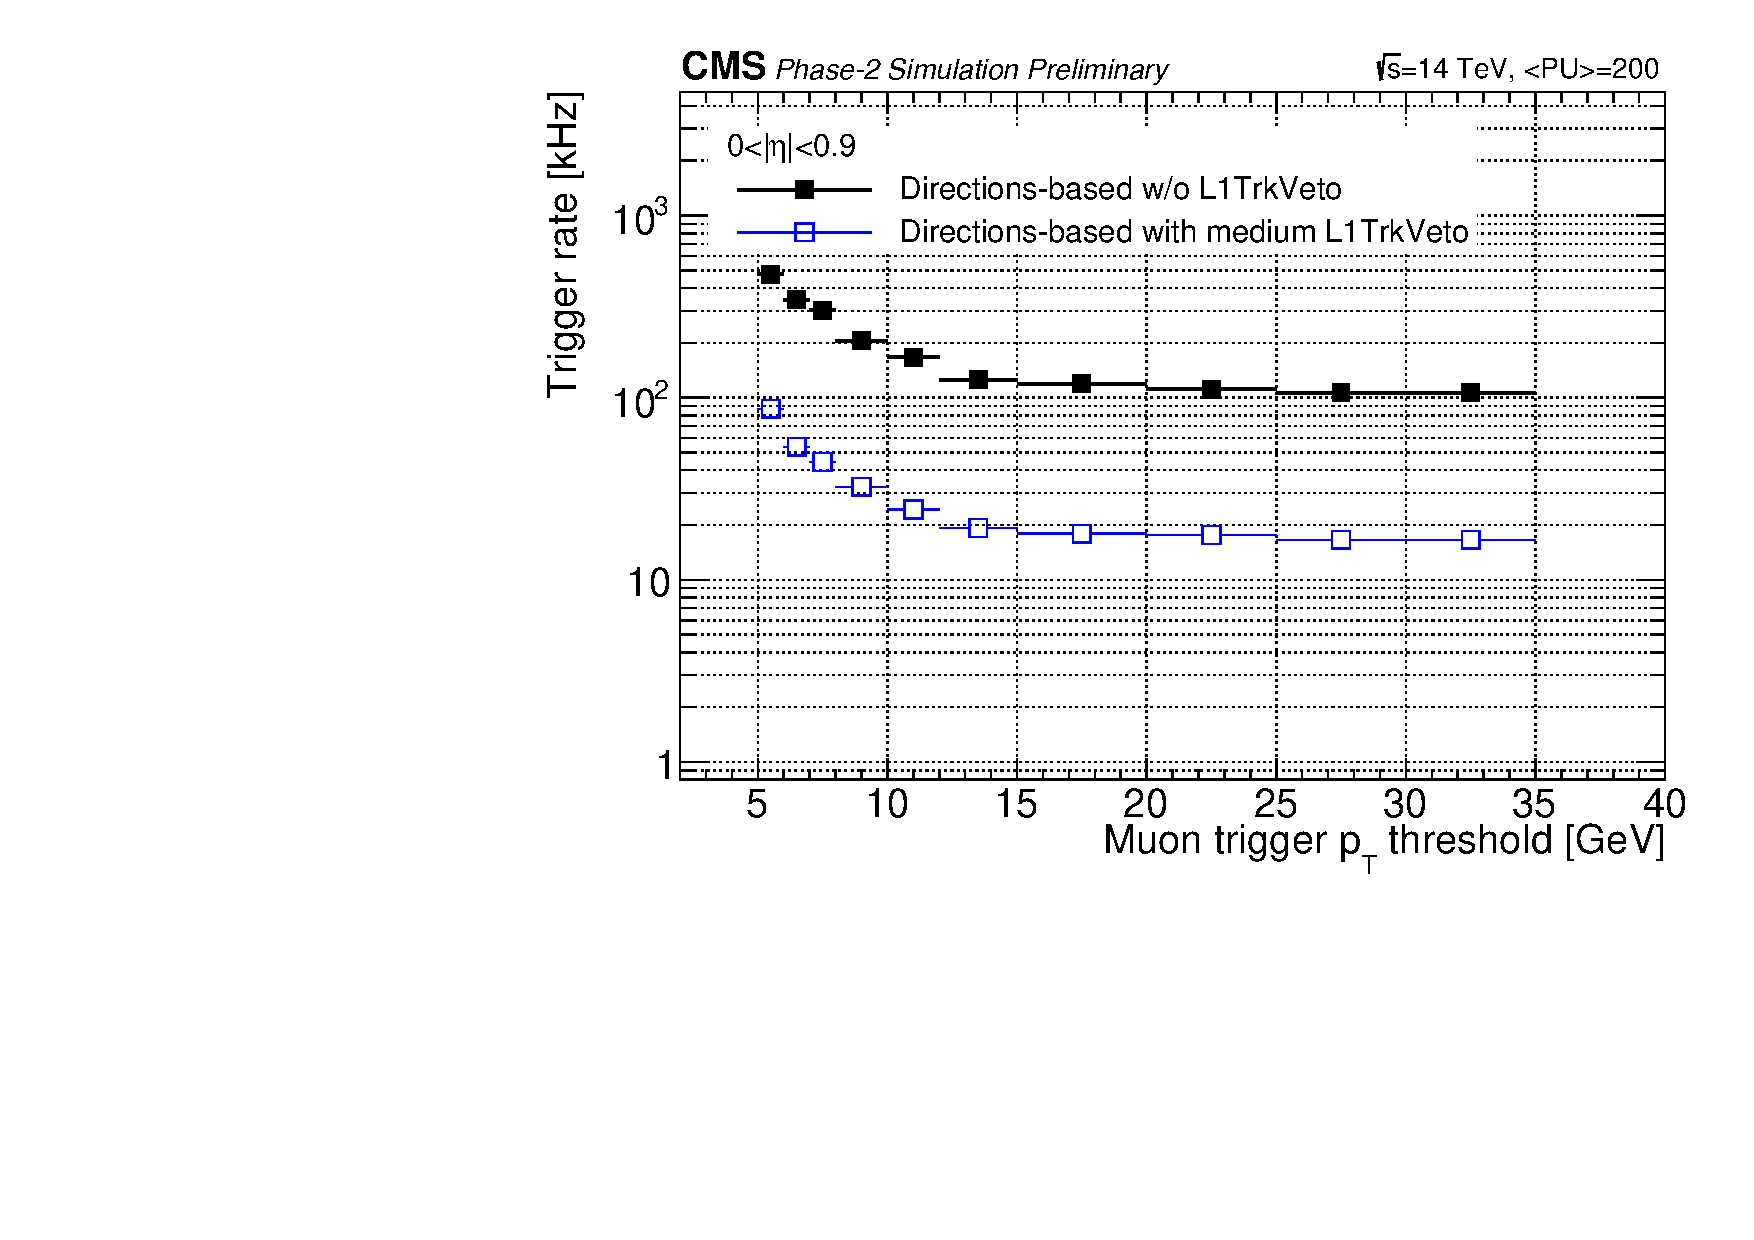
\includegraphics[width=0.47\textwidth]{figures/cmsupgrade/TDR-17-003_fig_7_11_a_Prompt_L1Mu_trigger_rate_pt__L1Mu__L1Mu2st__DisplacedL1MuDirectionBased_MB1_MB2_MB3_MB4_combined_eta0to0p9.pdf} \hfill
  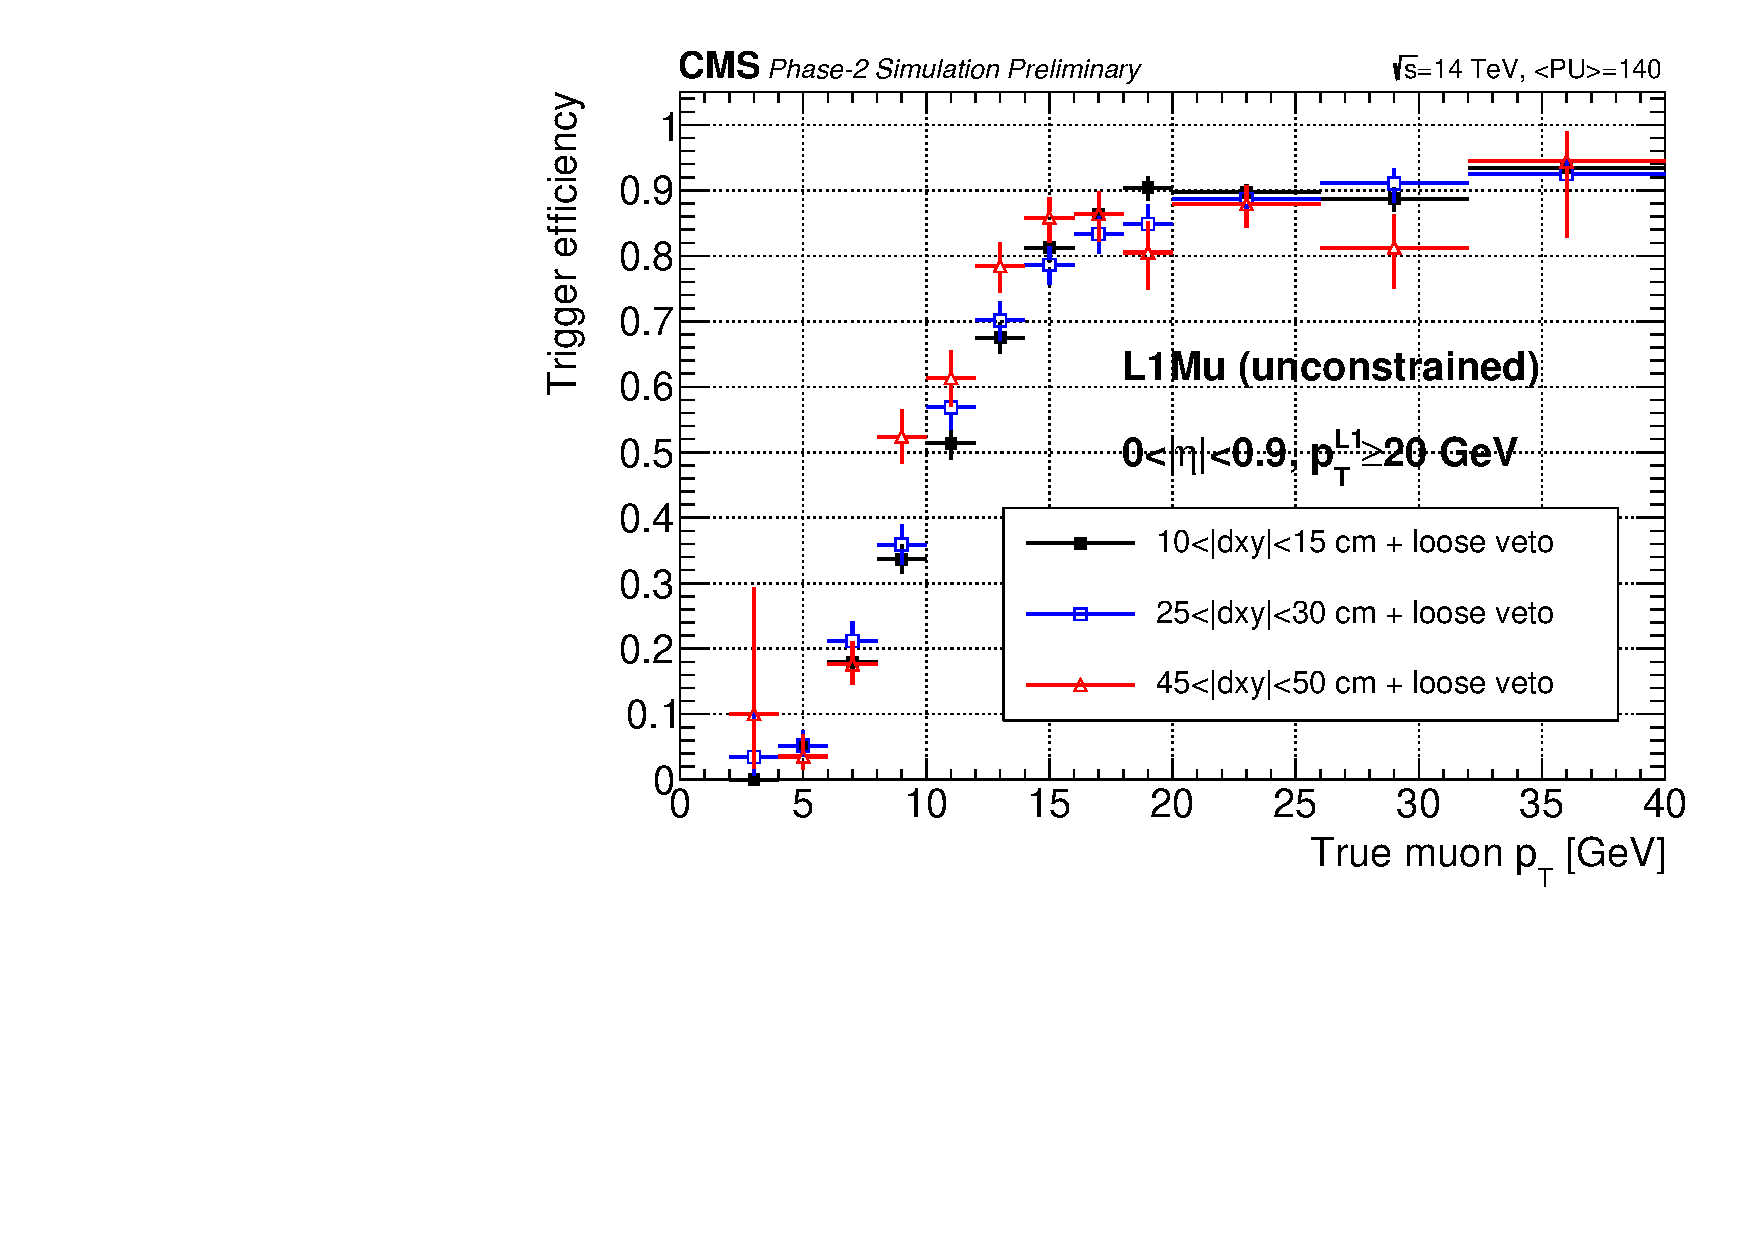
\includegraphics[width=0.47\textwidth]{figures/cmsupgrade/TDR-17-003_fig_7_11_b_L1MuonTDR2017Displaced_L1MuPt20_SimMuPt_DT1_DT2_DT3_DT4_combined_eta0to0p9_dxy5to50_looseVeto.pdf}
  \caption{L1 Muon trigger rate (left) and efficiency (right)
versus muon $\pt$ threshold for the barrel displaced muon algorithm~\cite{Lourenco:2283189}.}
  \label{fig:cmsL1mu}
\end{center}
\end{figure}


\paragraph{Reconstruction}

A dedicated muon reconstruction algorithm was designed for non-prompt muons that leave hits only in the muon system. This displaced stand-alone (DSA) algorithm is seeded by groups of track segments in the muon chambers. For each seed, a muon track is reconstructed with the same Kalman-filter technique as for the standard stand-alone (SA) muon reconstruction algorithm, but without constraining the interaction point. Figure~\ref{fig:perfDisplaced} (right) shows the distribution of the number of hits in the Run 2 and HL-LHC detectors for displaced muons. The impact of the new stations is clearly visible. The charge mis-identification probability is expected to further decrease with the additional hits.

\paragraph{Sensitivity Projection with a GMSB Model}

To study the impact on physics sensitivity, a particular gauge-mediated SUSY breaking (GMSB) model is selected where the displaced signature consists of a dimuon final state plus gravitinos, emerging from the decay of heavy long-lived sparticles (smuons), where the gravitinos escape detection. This maps to the direct pair production simplified model with neutral LLP decays to muon + invisible in Section~\ref{sec:proposal}. This signal can serve as a proxy for other models with two LLPs decaying into muons. The final-state signature is then given by two displaced, oppositely-charged muons and significant \met. Example long-lived particles with $c\tau=10, 100, 1000$~mm\,and several mass hypotheses (0.2, 0.5, 1~TeV) are simulated.

The main background for this search comes from multi-jet production (QCD), \ttbar~production, and Z/DY $\to\ell\ell$ events where large impact parameters are (mis)reconstructed. Cosmic-ray muons have been studied in Run 2 and these studies can be directly applied to Phase 2 running. 
In the barrel, they are efficiently rejected by the timing of the hits in the upper leg. Cosmic-ray muons do not originate at the vertex and therefore pass the upper-barrel sectors in reverse direction from outside in. The fraction of cosmic-ray muons in the endcaps is negligible.

Given the very low cross section of the signal process, it is essential to reduce the background efficiently. The best background discriminator is the impact parameter significance $d_0 / \sigma (d_0) \geq 5$. Given the signal kinematics, the muons from a signal process are expected to move in roughly opposite directions and \met can be expected to be larger than $50$~GeV. After this selection the signal efficiency is about 4--5\% for $c\tau \approx 1000$~mm, nearly independent of the smuon mass, and $10^{-5}$ -- $10^{-4}$ for QCD, \ttbar, and DY backgrounds.

In Figure~\ref{fig:displResults}, the expected exclusion limits are shown for the GMSB model in which the smuon is a (co-)next-to-lightest supersymmetric particle (NLSP, where ``LSP'' indicates the lightest supersymmetric particle), for the predicted cross section as well as for a factor 100 larger cross section. The exclusion limits are shown as functions of smuon mass in Figure~\ref{fig:displResults} (left) and decay length in Figure~\ref{fig:displResults} (right).

\begin{figure}[t]\begin{center}
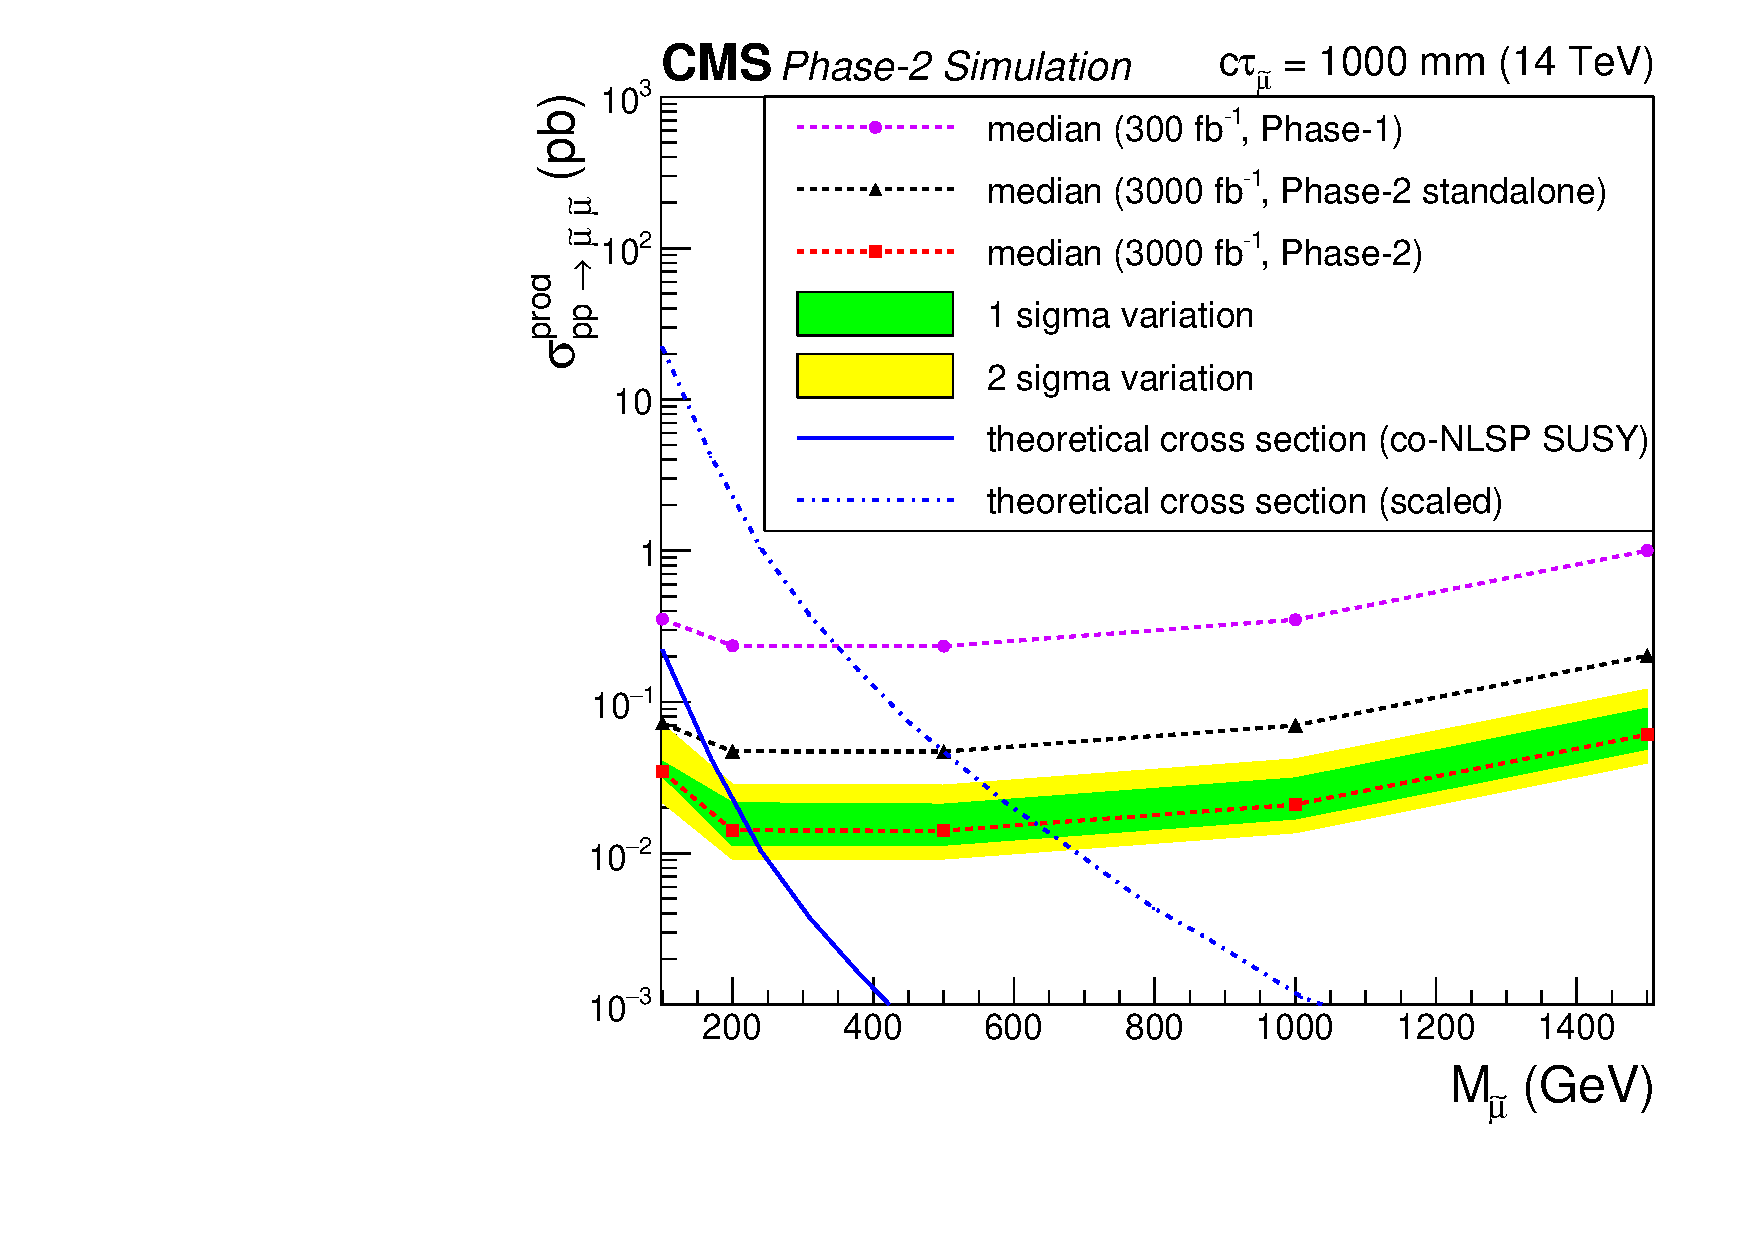
\includegraphics[width=0.47\textwidth]{figures/LimitComparison_withStandAloneEff.pdf}
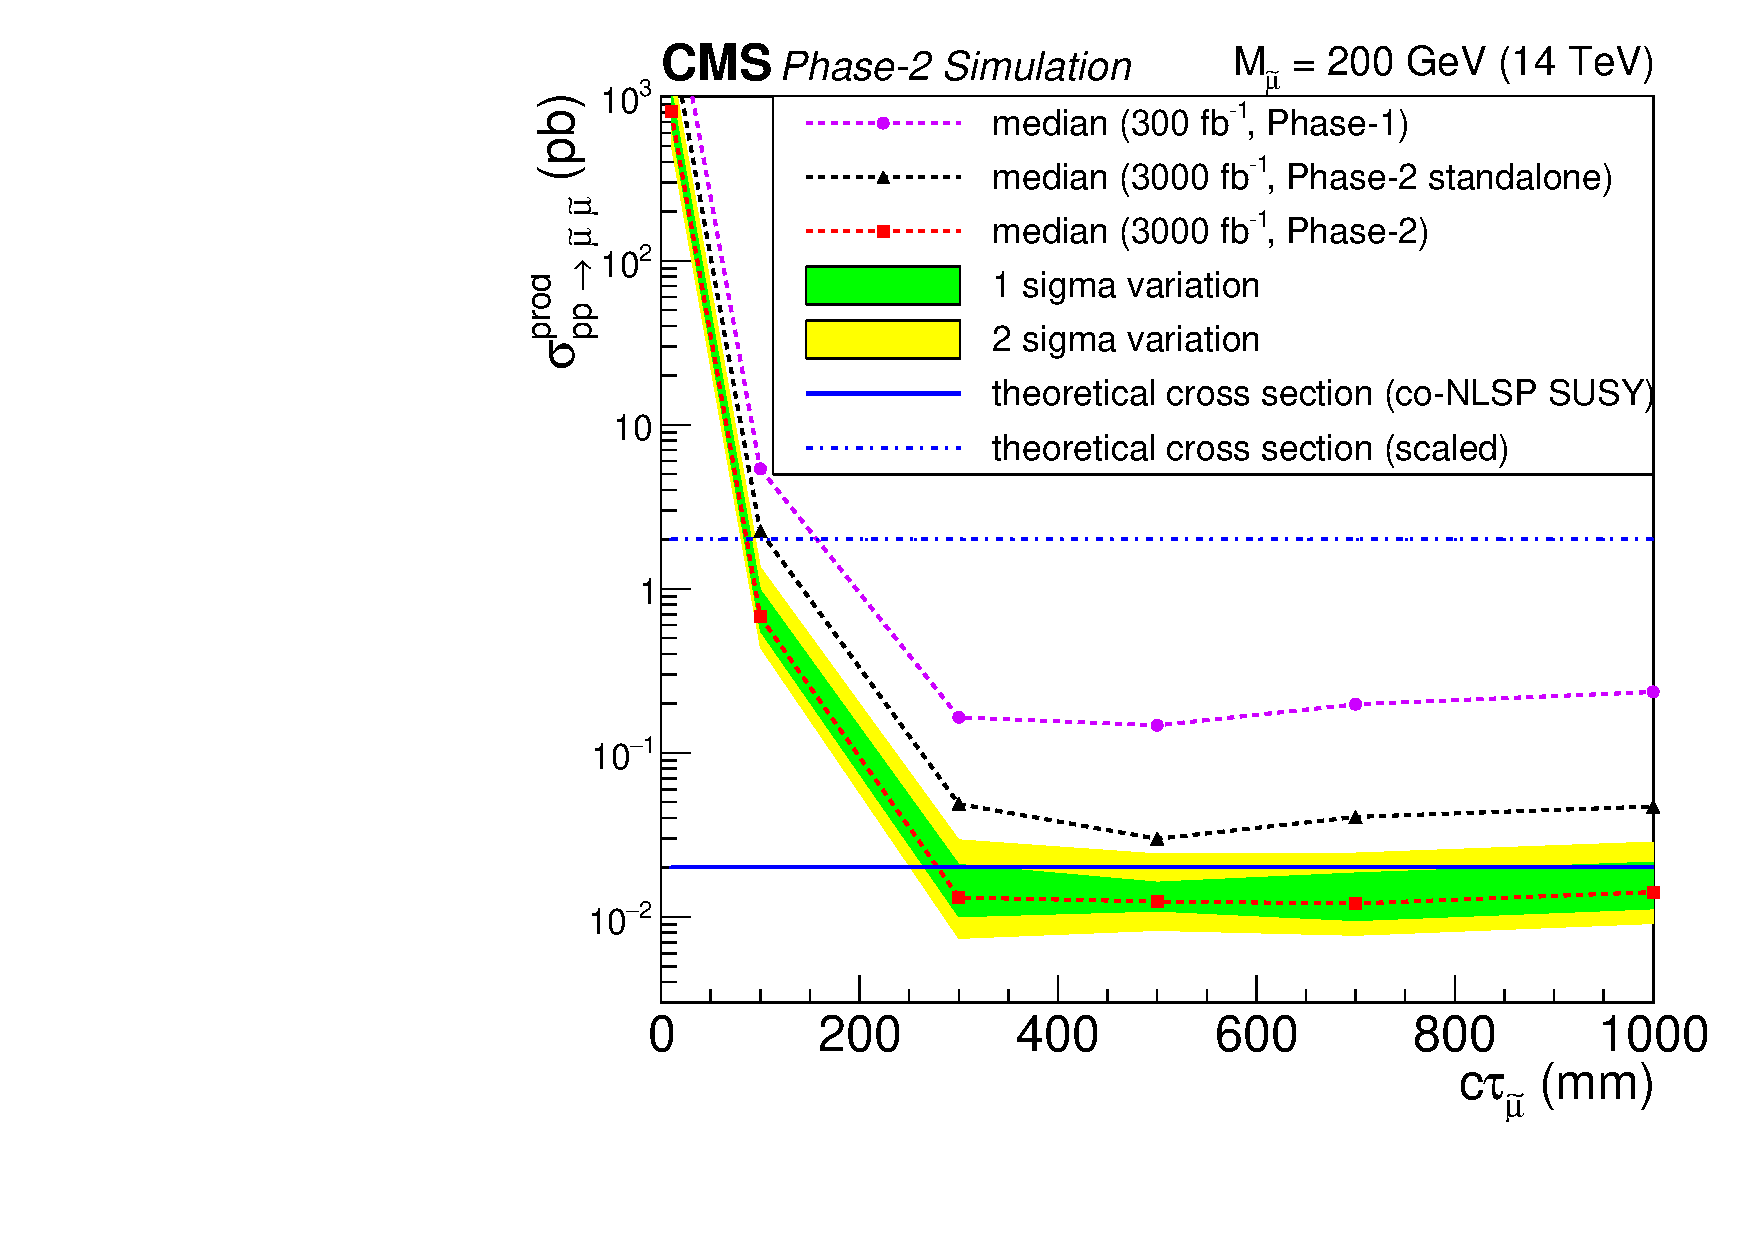
\includegraphics[width=0.47\textwidth]{figures/LimitComparison_asfuncofCtau.pdf}
\caption{The 95\% C.L. projected upper limits at CMS for $q \bar q \to \widetilde{\mu} \widetilde{\mu}, \widetilde{\mu}\rightarrow \mu\widetilde{G}$ for various mass hypotheses for $c\tau$ = 1~m (left), and as a function of the decay length for $m_{\widetilde{\mu}}$ = 200~GeV (right). In both panels, the theoretical cross section for the specific model is represented by the blue solid line. For different SUSY breaking scales, tan~$\beta$ or otherwise modified parameters, the cross sections may be 100 times larger, reflected by the blue dash-dotted line. Green (yellow) shaded bands show the one (two) sigma range of variation of the expected 95\% C.L. limits. Phase 2 results with an average of 200 pile-up collisions per bunch crossing and an integrated luminosity of $300$\fbinv are compared to results obtained with $300$\fbinv. The black line shows the sensitivity without the DSA algorithm, which reduces the reconstruction efficiency by a factor three~\cite{Lourenco:2283189}.
 }
\label{fig:displResults}
\end{center}
\end{figure}

The sensitivity depends on $c\tau$ because shorter decay lengths shift the signal closer to background. In Figure~\ref{fig:displResults} (right), the resulting physics sensitivities in terms of production cross section for the HL-LHC, normalized to $3000$\fbinv, are shown for the dedicated reconstruction of displaced muons and for the standard reconstruction. Also shown is the expected sensitivity at the end of Phase 1. Systematic uncertainties for the Phase 1 scenario are taken from current Run 2 analyses and adapted for expected HL-LHC conditions based on the assumptions of reduced systematics described in Ref.~\cite{FTR-16-005}. Clearly, only the HL-LHC will allow this process to be studied. The expected exclusion limit is around 200~GeV for $c\tau = 1000$~mm with 3000\fbinv. This also illustrates the importance of keeping lepton trigger thresholds at several tens of GeV, even in the environment of 200 pile-up interactions per bunch crossing.
Similarly, the discovery sensitivity is assessed assuming that a signal is present in data, and is shown as a function of smuon mass in Figure~\ref{fig:displResultsSensitiviy} (left) and decay length in Figure~\ref{fig:displResultsSensitiviy} (right).

\begin{figure}[t]\begin{center}
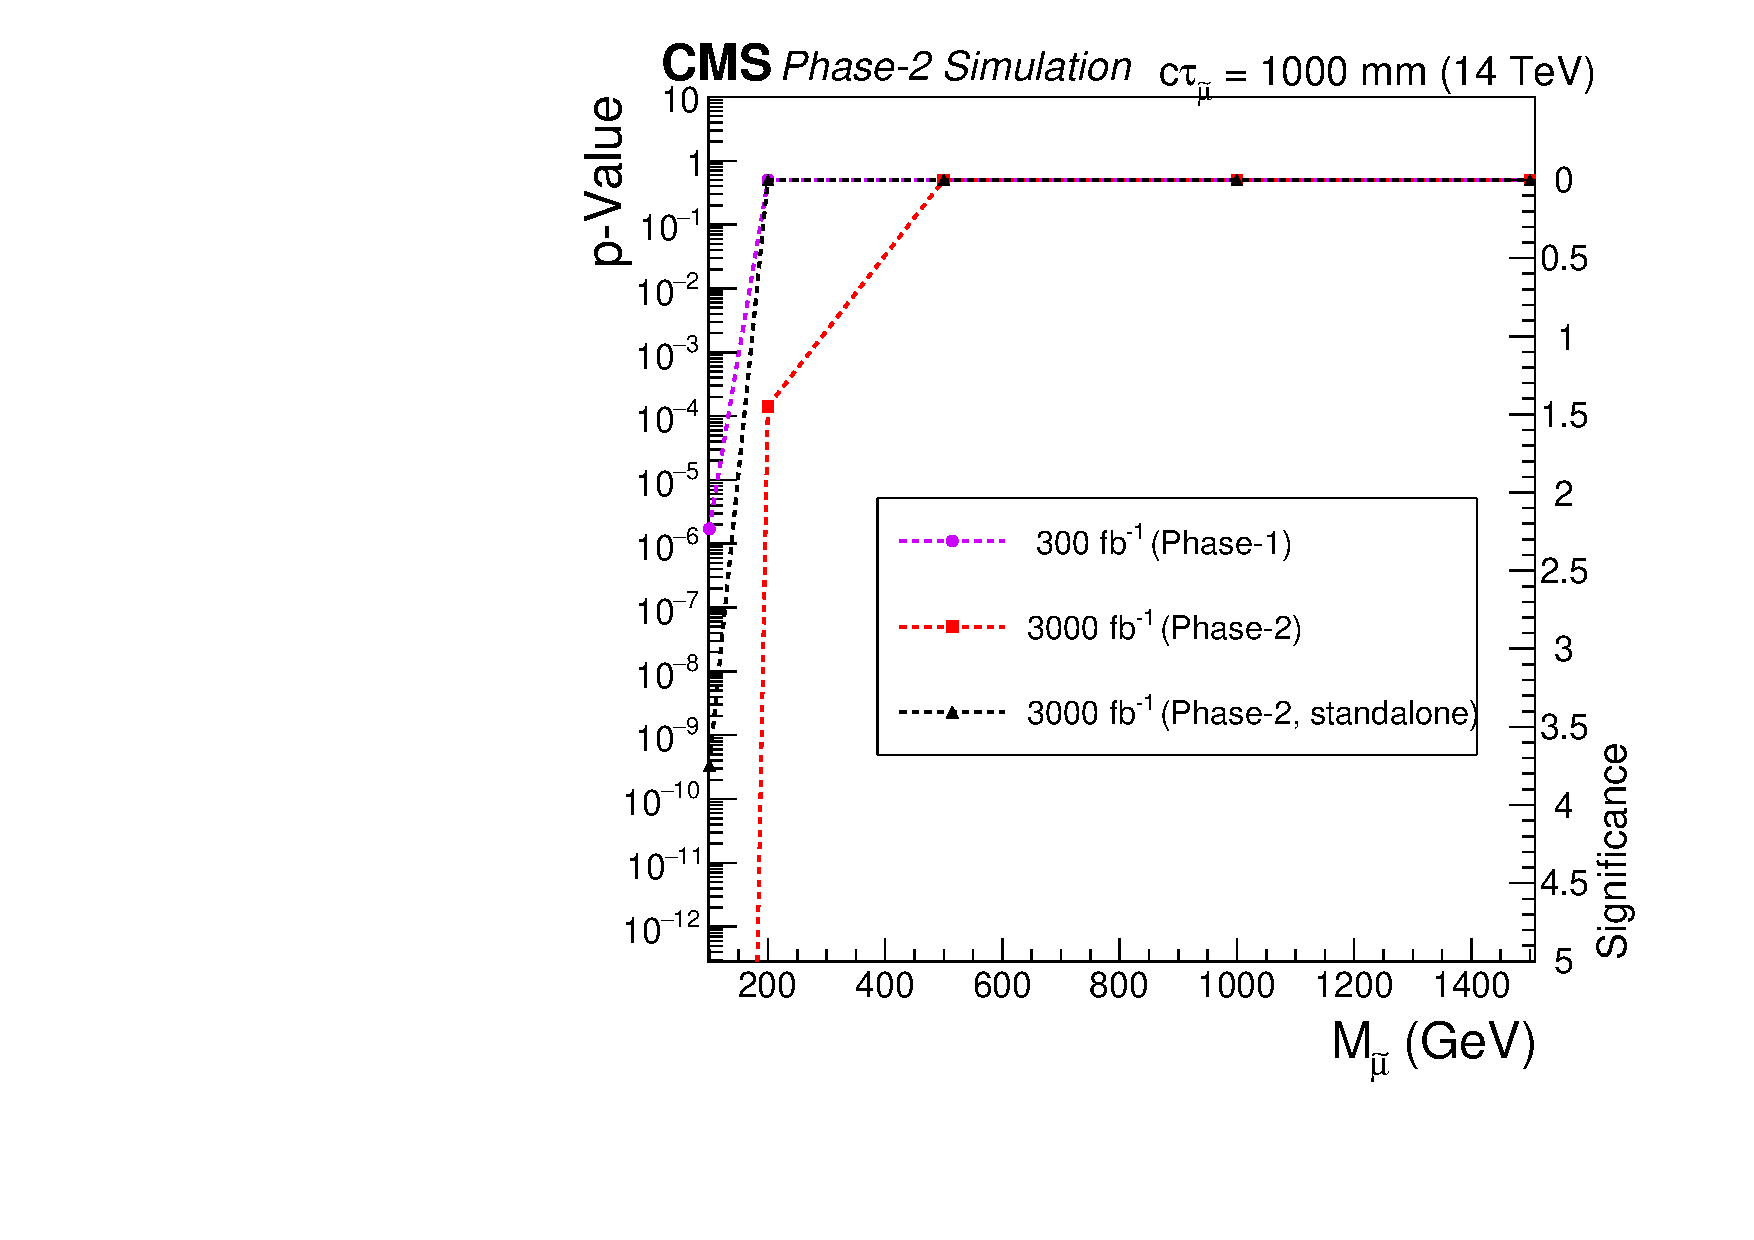
\includegraphics[width=0.47\textwidth]{figures/SignificanceComp.pdf}
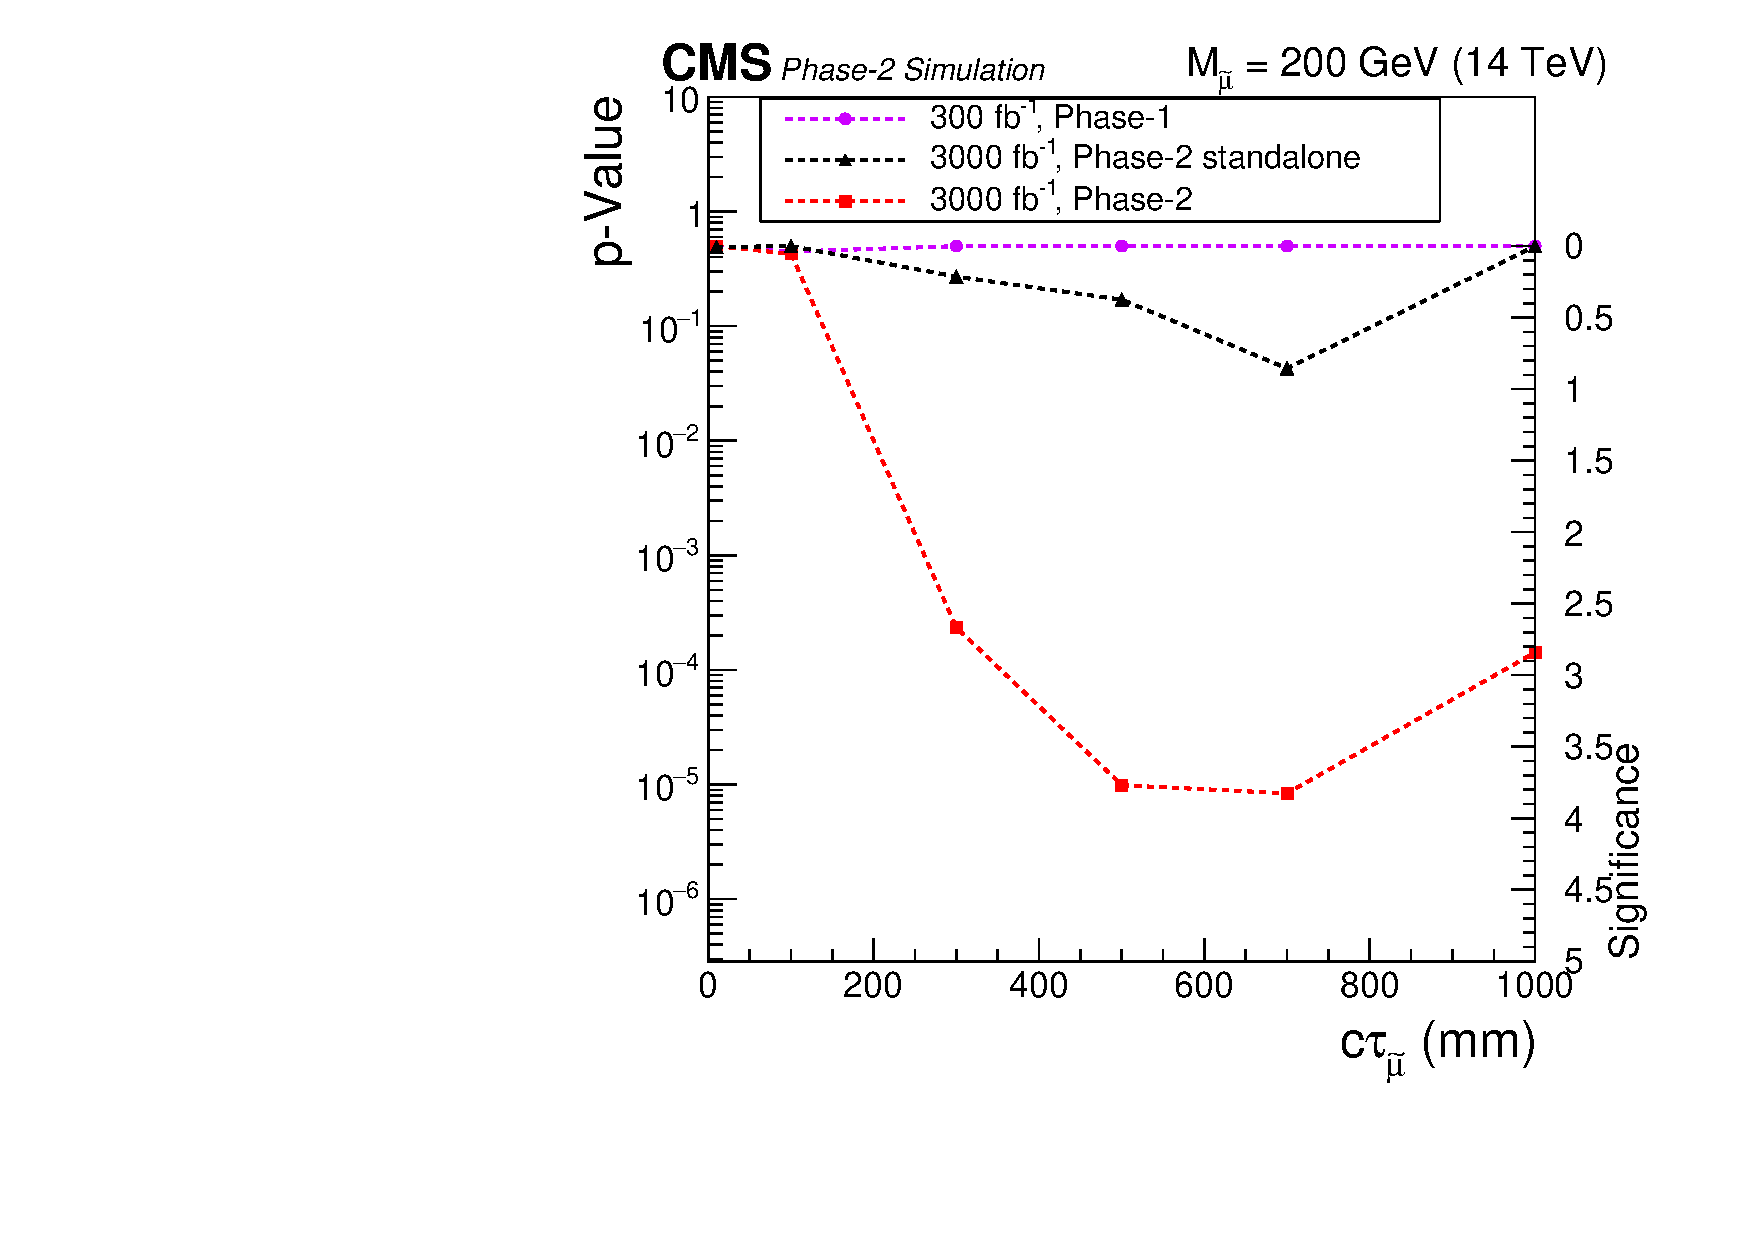
\includegraphics[width=0.47\textwidth]{figures/SignificanceComp_asfuncofCtau.pdf}
\caption{The projected discovery sensitivity at CMS for  $q \bar q \to \widetilde{\mu} \widetilde{\mu}, \widetilde{\mu}\rightarrow \mu\widetilde{G}$ for various mass hypotheses and $c\tau$ = 1~m (left) and as a function of the decay length for $m_{\widetilde{\mu}}$ = 200~GeV (right). Together with the discovery sensitivity the corresponding $p$-value is shown. Phase 2 results with an average of 200 pile-up interactions per bunch crossing and an integrated luminosity of 3000\fbinv are compared to results obtained with 300\fbinv. The black line shows the sensitivity without the DSA algorithm, which reduces the reconstruction efficiency by a factor three~\cite{henningkeller2018}.
 }
\label{fig:displResultsSensitiviy}
\end{center}
\end{figure}


\paragraph{Sensitivity Projection with a Dark SUSY Model}
The analysis presented above was reinterpreted using a Dark SUSY model (\cite{Baumgart:2009tn,Falkowski:2010cm}), in which an additional dark $U_D(1)$ symmetry is added as a supersymmetric SM extension. Breaking this symmetry gives rise to an additional massive boson, the so-called dark photon ($\gamma_D$), which couples to SM particles via a small kinetic mixing parameter $\epsilon$. If $\epsilon$ is very weak, the lifetime of the dark photon can range from a few millimeters up to several meters. The lower $\epsilon$, the longer is the dark photon lifetime which then decays displaced from the primary vertex. A golden channel for such searches is the decay to displaced muons.

In the model studied here~\cite{CMS-PAS-FTR-18-002}, dark photons are produced in cascade decays of the SM Higgs boson that would first decay to a pair of MSSM-like lightest neutralinos ($n_1$), each of which can decay further to a dark sector neutralino ($n_D$) and the dark photon.

For the branching fraction BR$(H \to 2\gamma_D + \mathrm{X})$, where X denotes the particles produced in the decay of the SM Higgs boson apart
from the dark photons, $20\%$ is used. Neutralino masses $m(n_1) =
50~\mathrm{GeV}$ and $m(n_D) = 1~\mathrm{GeV}$ are assumed. Final states with two
and four muons are included in the analysis. In the former case, one dark photon decays to a pair of muons while the other dark photon decays
to some other fermions (2-muon final state). In the latter case, both dark photons decay to muon pairs (4-muon final state).

The main background for this search comes from multi-jet production (QCD), ttbar~production,
and Z/DY $\to\ell\ell$ events  where large impact parameters are (mis)reconstructed. Cosmic ray muons can travel through the detector far away from the primary vertex and mimic the signature of displaced muons.
However, thanks to their striking detector signature, muons from cosmic rays can be suppressed by rejecting back-to-back kinematics.

For each event, at least two DSA muons are required. If more than two, the ones with the
highest $\pt$ are chosen. The two muons must have opposite charge ($q_{\mu,1} \cdot q_{\mu,2} = -1$) and must be separated by $\Delta R = \sqrt{\Delta \phi^2 + \Delta
\eta^2} > 0.05$. The three-dimensional angle between the two displaced muons is required to be less than $\pi - 0.05$ (not back-to-back) in order to suppress cosmic
ray backgrounds. Additionally, $\ptmiss \geq 50~\mathrm{GeV}$ is imposed to account for the dark neutralinos escaping the detector without leaving any signal.

In order to discriminate between background and signal, the three-dimensional distance from the primary vertex to the point of closest approach of the extrapolated
displaced muon track, called $R_{\text{Muon}}$, is used.
The event yield after full event selection of both selected muons as a function of $R_{\rm Muon-1}$ and $R_{\rm Muon-2}$ is used to search for the signal. The left panel of Figure~\ref{fig:DarkPhoton_Distr_Disc} shows $R_{\rm Muon-1}$ of the first selected muon for signal and background samples.

\begin{figure}[hbtp]
\begin{center}
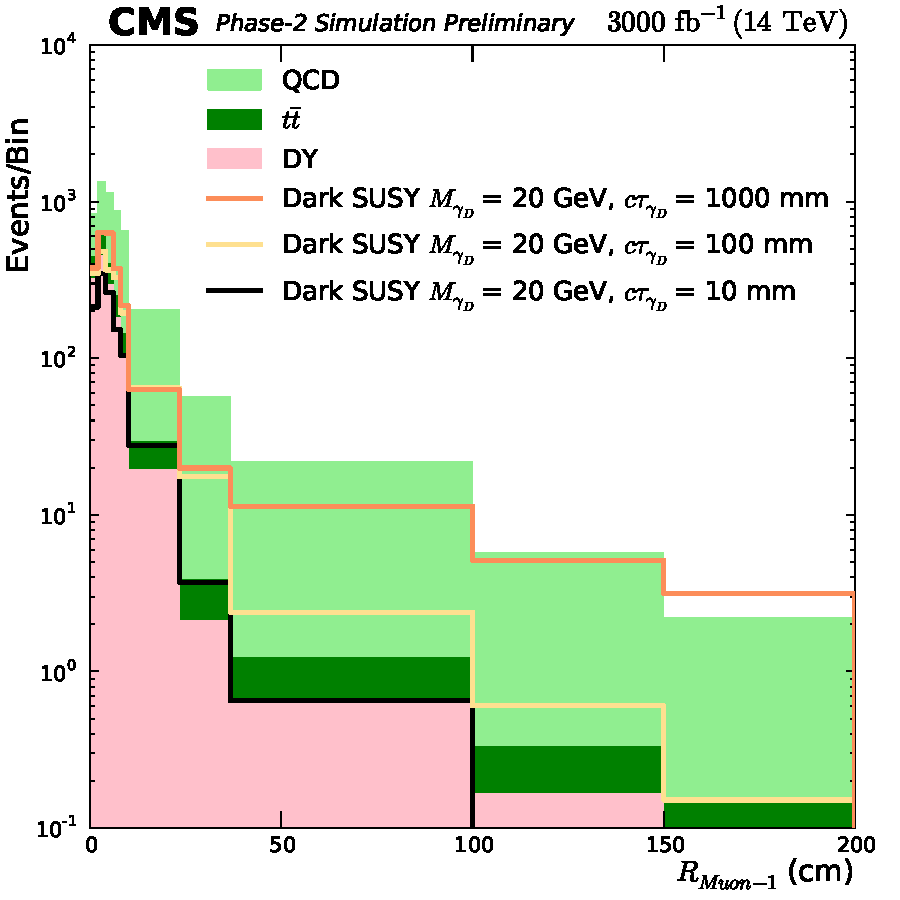
\includegraphics[width=0.45\textwidth]{tex/figures/cmsupgrade/FTR-18-002/DarkPhoton_Distribution}
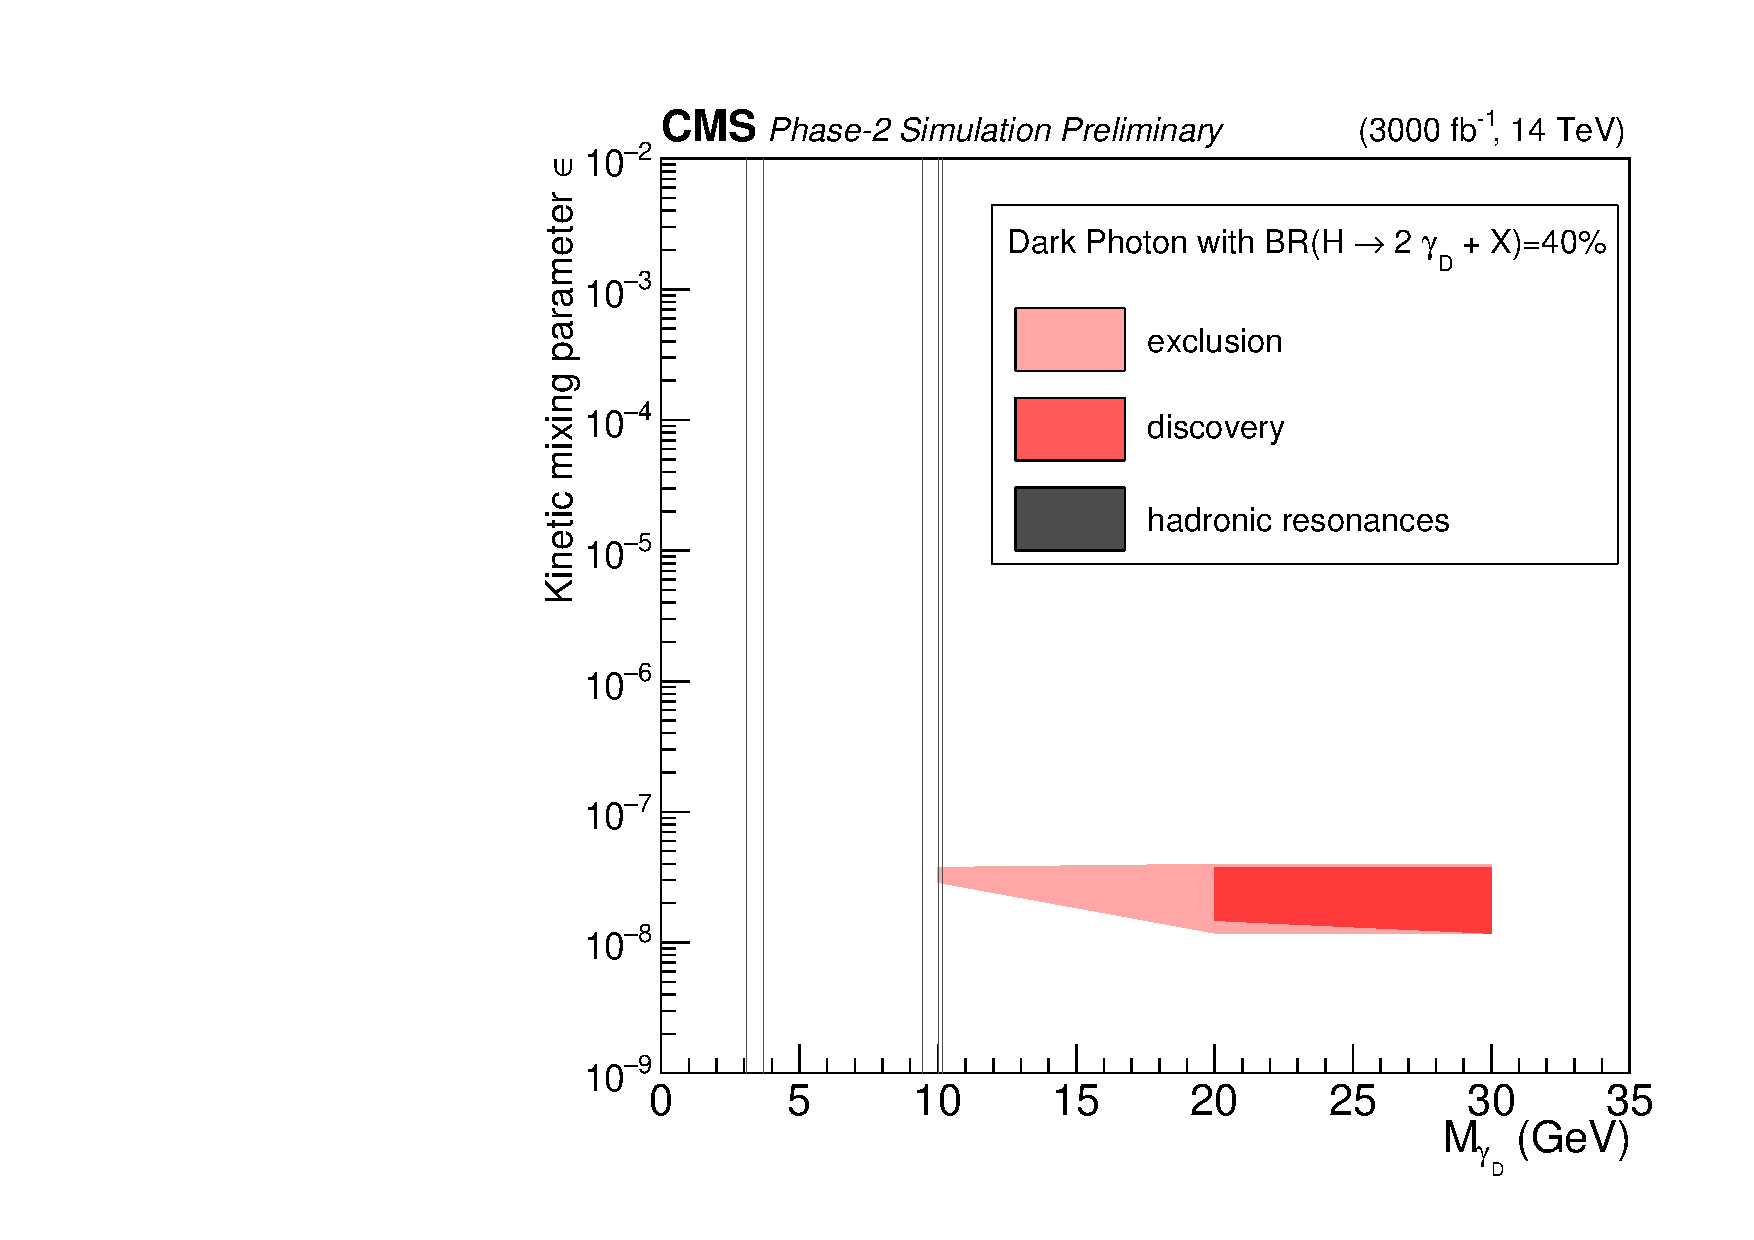
\includegraphics[width=0.45\textwidth]{tex/figures/cmsupgrade/FTR-18-002/Paramspace_merged.pdf}
 \caption{{\bf Left:} distance of the closest approach of the displaced muon track with maximum $\pt$  to the primary interaction vertex, $R_{\rm Muon-1}$, for signal and background after the final event selection.
{\bf Right:}Parameter scan in the $\epsilon-m_{\gamma_D}$ plane. The grey lines indicate the regions of narrow hadronic resonances where the analysis does not claim any sensitivity~\cite{CMS-PAS-FTR-18-002}.}
\label{fig:DarkPhoton_Distr_Disc}
\end{center}
\end{figure}


%%% Sensitivity in exclusion and discovery
The search is performed using a simple counting experiment approach. In presence of the expected signal, significance of the corresponding event excess over the expected background is assessed using the likelihood method.
In order to evaluate the discovery sensitivity the same input is used as in the limit calculation, now with the assumption that one would have such a signal in the data. The discovery sensitivity is shown in the two-dimensional $m_{\gamma_D}$-$c\tau$ plane in the right panel of Figure~\ref{fig:DarkPhoton_Distr_Disc}. This search is sensitive to large decay length of the dark photon.

In absence of a signal, upper limits at $95\%$ C.L. are obtained on a signal
event yield with respect to the one expected for the considered model. A Bayesian method with a uniform prior for the signal event rate is used and the nuisance
parameters associated with the systematic uncertainties are modeled with log-normal distributions.
The resulting limits for the Dark SUSY models are depicted in Figure \ref{fig:NewCompLimit_DarkPhoton}. While the results shown in the left panel of Figure~\ref{fig:NewCompLimit_DarkPhoton} are for a dark photon with a decay length of $1~\mathrm{m}$ as a function of the dark photon mass, the right panel of Figure~\ref{fig:NewCompLimit_DarkPhoton} shows the results for a dark photon mass of $20~\mathrm{GeV}$ as a function of the decay length~\cite{CMS-PAS-FTR-18-002}.



\begin{figure}[hbtp]
\begin{center}
\includegraphics[width=0.45\textwidth]{tex/figures/cmsupgrade/FTR-18-002/LimitComp_Ratio_DarkPhotons.pdf}
\includegraphics[width=0.45\textwidth]{tex/figures/cmsupgrade/FTR-18-002/LimitComp_Ratio_asfuncofCtau_DarkPhotons.pdf}
 \caption{Upper limits at $95\%$ C.L. on production cross section $\sigma / \sigma_{\text{theory}}$ for various dark photon mass hypotheses and a fixed decay length of $c\tau = 1000$~mm (a) and a fixed mass of $M_{\gamma_D} = 20$~GeV (b). Green and yellow shaded bands show the one and two sigma range of variation of the expected $95\%$ C.L. limits, respectively. The grey lines indicate the regions of narrow hadronic resonances where the analysis does not claim any sensitivity~\cite{CMS-PAS-FTR-18-002}.}
\label{fig:NewCompLimit_DarkPhoton}
\end{center}
\end{figure}


\subsubsection{Displaced Photons at CMS}


A number of new physics scenarios predict new particles that, upon decay, result in displaced photons in the final state (see Section~\ref{sec:proposal} and Section~\ref{subsec:dphotons}). At the CMS experiment, with the scintillating crystal design of the ECAL that provides excellent resolution but lacks pointing capability, the photon arrival time in the ECAL is the main observable used to distinguish signal from background in displaced photon searches.

One benchmark model for displaced photon searches is the GMSB model where the lightest neutralino ($\tilde{\chi}_0^1$) is the next-to-lightest supersymmetric particle, can be long-lived, and decays to a photon and a gravitino ($\tilde{G}$), which is the LSP, as illustrated in Figure~\ref{fig:cmsupgrade_photon} (left). For a long-lived neutralino, the photon from the $\tilde{\chi}_0^1\to\tilde{G}+\gamma$ decay is produced at the $\tilde{\chi}_0^1$ decay vertex, at some distance from the beam line, and reaches the detector at a time later than that of prompt, relativistic particles produced at the interaction point. The time of arrival of the photon at the detector can be used to discriminate the signal from the background. The aforementioned upgrade to the ECAL electronics in the barrel region, and the HGCAL upgrade in the endcaps, will improve photon timing resolution at HL-LHC by an order of magnitude to as little as $\sim30$~ps for photons with $\pt$ of tens of GeV or above, hence significantly improve the experimental reach of displaced photon searches.

Moreover, the proposed MIP Timing Detector (MTD) will be able to provide another dimension of information to reconstruct LLP decays. The time of flight of the photon inside the detector is the sum of the time of flight of the neutralino before its decay and the time of flight of the photon itself, until it reaches the detector. Since the neutralino is a massive particle the latter is clearly negligible with respect to the former. In order to be sensitive to short neutralino lifetimes of order 1~cm, the performance of the measurement of the photon time of flight is a crucial ingredient of the analysis. Therefore, the excellent resolution of the MTD apparatus can be exploited to determine with high accuracy the time of flight of the neutralino, and similarly the photon, also in case of a short lifetime.

An analysis has been performed at generator level in order to evaluate the sensitivity power of a search for displaced photons at CMS in the scenario where a 30~ps timing resolution is available from the MTD~\cite{MTD_TP}. The events were generated with Pythia 8~\cite{Sjostrand:2007gs}, exploring neutralino lifetimes ($c\tau$) in the range 0.1--300~cm. The values of the $\Lambda$ scale parameter were considered in the range 100--500 TeV, which is relevant for this model to be consistent with the observation of a 125~GeV Higgs boson. After requiring the neutralino to decay within the CMS ECAL acceptance and the photon energy being above a ``trigger-like'' threshold, the generator-level photon time of flight was smeared according to the expected experimental resolutions. A cutoff at a photon time greater than 3$\sigma$ of the timing resolution is applied and the ``signal region'' is assumed to be background free to estimate the sensitivity. The signal efficiency of such a requirement is computed and translated, assuming the theoretical cross sections provided in Ref.~\cite{Strassler:2006im}, to an upper limit, at 95\% C.L., on the production cross section of the $\tilde{\chi}_0^1 \to \tilde{G} + \gamma$ process.

In Figure~\ref{fig:cmsupgrade_photon} (right), the analysis sensitivity in terms of the $\Lambda$ scale (and therefore of the neutralino mass) and lifetime is shown for three different assumptions on the timing resolution. The 300~ps resolution is representative of the time-of-flight resolution (TOF) consistent with current CMS detector performance. The 180~ps resolution is representative of the TOF resolution of the upgraded CMS detector without the MTD, in which case the TOF measurement will be dominated by the time spread of the luminous region. The vertex timing provided by the MTD detector will bring the TOF resolution to about 30~ps. As visible in the figure, a full-scope upgrade of the CMS detector with photon and track timing will provide a dramatic increase in sensitivity at short lifetimes and high masses, even with the first $300\,\,\mathrm{fb}^{-1}$ of integrated luminosity.

\begin{figure}[t]\begin{center}
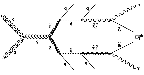
\includegraphics[width=0.47\textwidth]{figures/MTD/diagram.pdf}
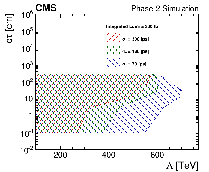
\includegraphics[width=0.47\textwidth]{figures/MTD/Limits_excl_2D_ComparingRes.pdf}
\caption{
{\bf Left:} diagrams for a SUSY process that results in a diphoton final state through gluino production at the LHC. {\bf Right:} sensitivity to GMSB $\tilde{\chi}_0^1 \to \tilde{G} + \gamma$ signals expressed in terms of neutralino lifetimes for 300, 180 and 30~ps resolution, corresponding to the current detector, the HL-LHC detector with photon timing without MTD and with MTD, respectively~\cite{MTD_TP}.
}
\label{fig:cmsupgrade_photon}
\end{center}
\end{figure}

\subsubsection{Displaced Jets in ATLAS}

%{\bf \textcolor{red}{[JB: Can this section be expanded a bit?  The discussion assumes a lot of knowledge that will be unclear to someone not in ATLAS.]}}

Neutral long-lived particles that can decay into jets displaced from the proton-proton interaction point arise in many BSM theories (see Chapter~\ref{sec:simplifiedmodel} for an extensive discussion). For example, in hidden sector models a new set of particles and forces is proposed that is weakly coupled to the SM via a communicator particle. The hidden sector is otherwise invisible to the SM sector, but its particles (some of which can be long-lived) may decay to SM particles via the communicator. The lifetimes of these LLPs are typically unconstrained and could be long enough for the LLPs to decay inside the ATLAS detector volume. Such particles produce unique signatures which may have been overlooked by more traditional searches for new physics. One ATLAS search for such displaced jet signatures focuses on LLPs which decay in the ATLAS hadronic calorimeter (HCal) and consequently deposit most of their energy there and very little or none in the electromagnetic calorimeter, and also have few or no charged tracks pointing at the hadronic energy deposits. A signature-driven trigger that optimizes the acceptance for this class of events is required for the online selection.

The existing ATLAS analysis described in Section~\ref{subsec:djets} can likely be improved by planned upgrades by using HCal information splitting the B-C layers in the calorimeter to identify the LLP decay position. %{\bf \textcolor{red}{[JB: What are the B-C layers?  Are they something new for the upgrade?  How does this change from now till upgrade time?]}}
The splitting between B-C layers will provide more information on the longitudinal shower profile, see~Figure~\ref{fig:Caloratio}.

This analysis uses a hidden sector benchmark model and considers the decay of a heavy boson to two long-lived neutral scalars; this maps to the simplified model with Higgs boson production of hadronically decaying LLPs in Section~\ref{sec:proposal}. The heavy scalar bosons decaying into LLPs have masses ranging from 125 GeV to 1000 GeV, and the LLP scalars have masses ranging between 5 GeV and 400 GeV.
Background processes, dominated by QCD dijet production, are suppressed in this analysis by requiring both scalars to decay  in the calorimeter. Final results of the analysis are pending.

\begin{figure}[hbtp]
\begin{center}
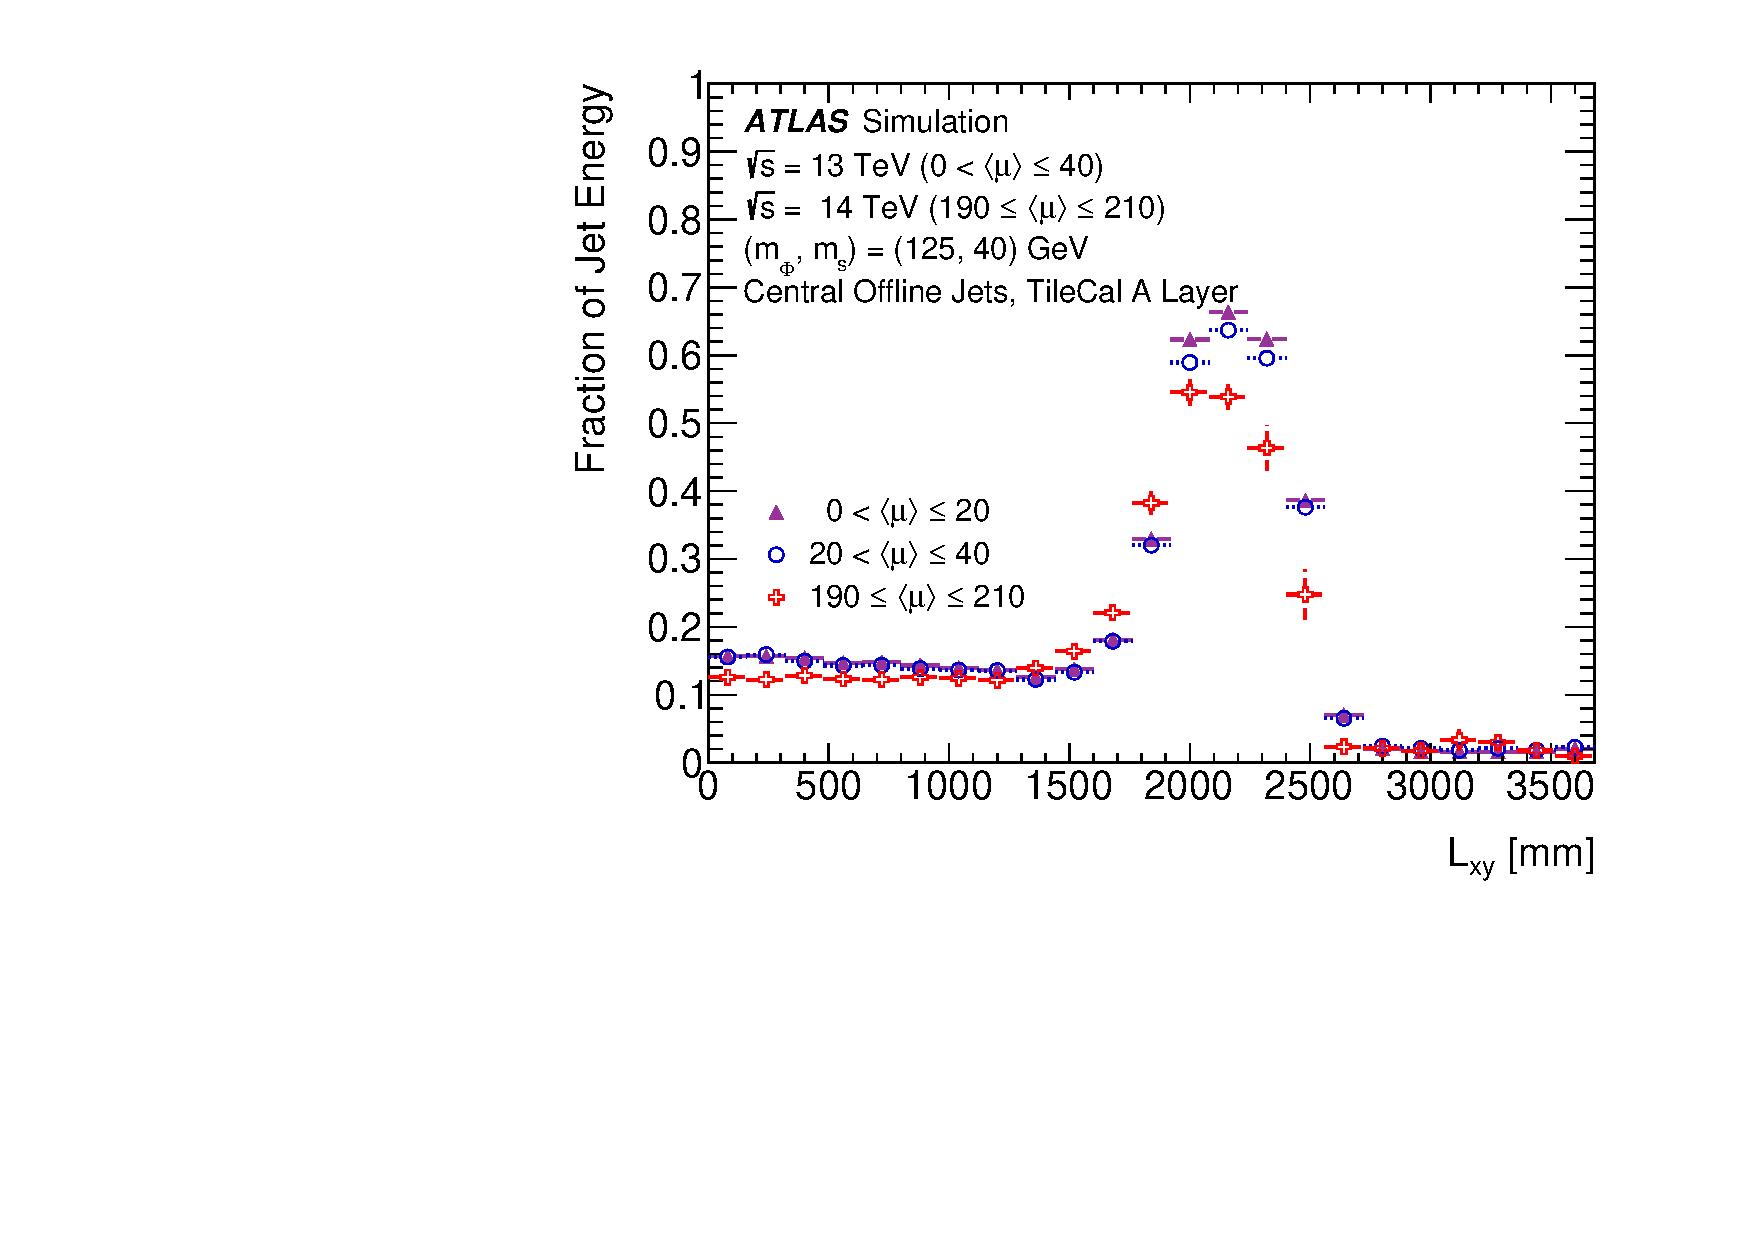
\includegraphics[width=0.47\textwidth]{figures/caloratio1.pdf}
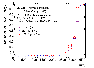
\includegraphics[width=0.47\textwidth]{figures/caloratio2.pdf}\\
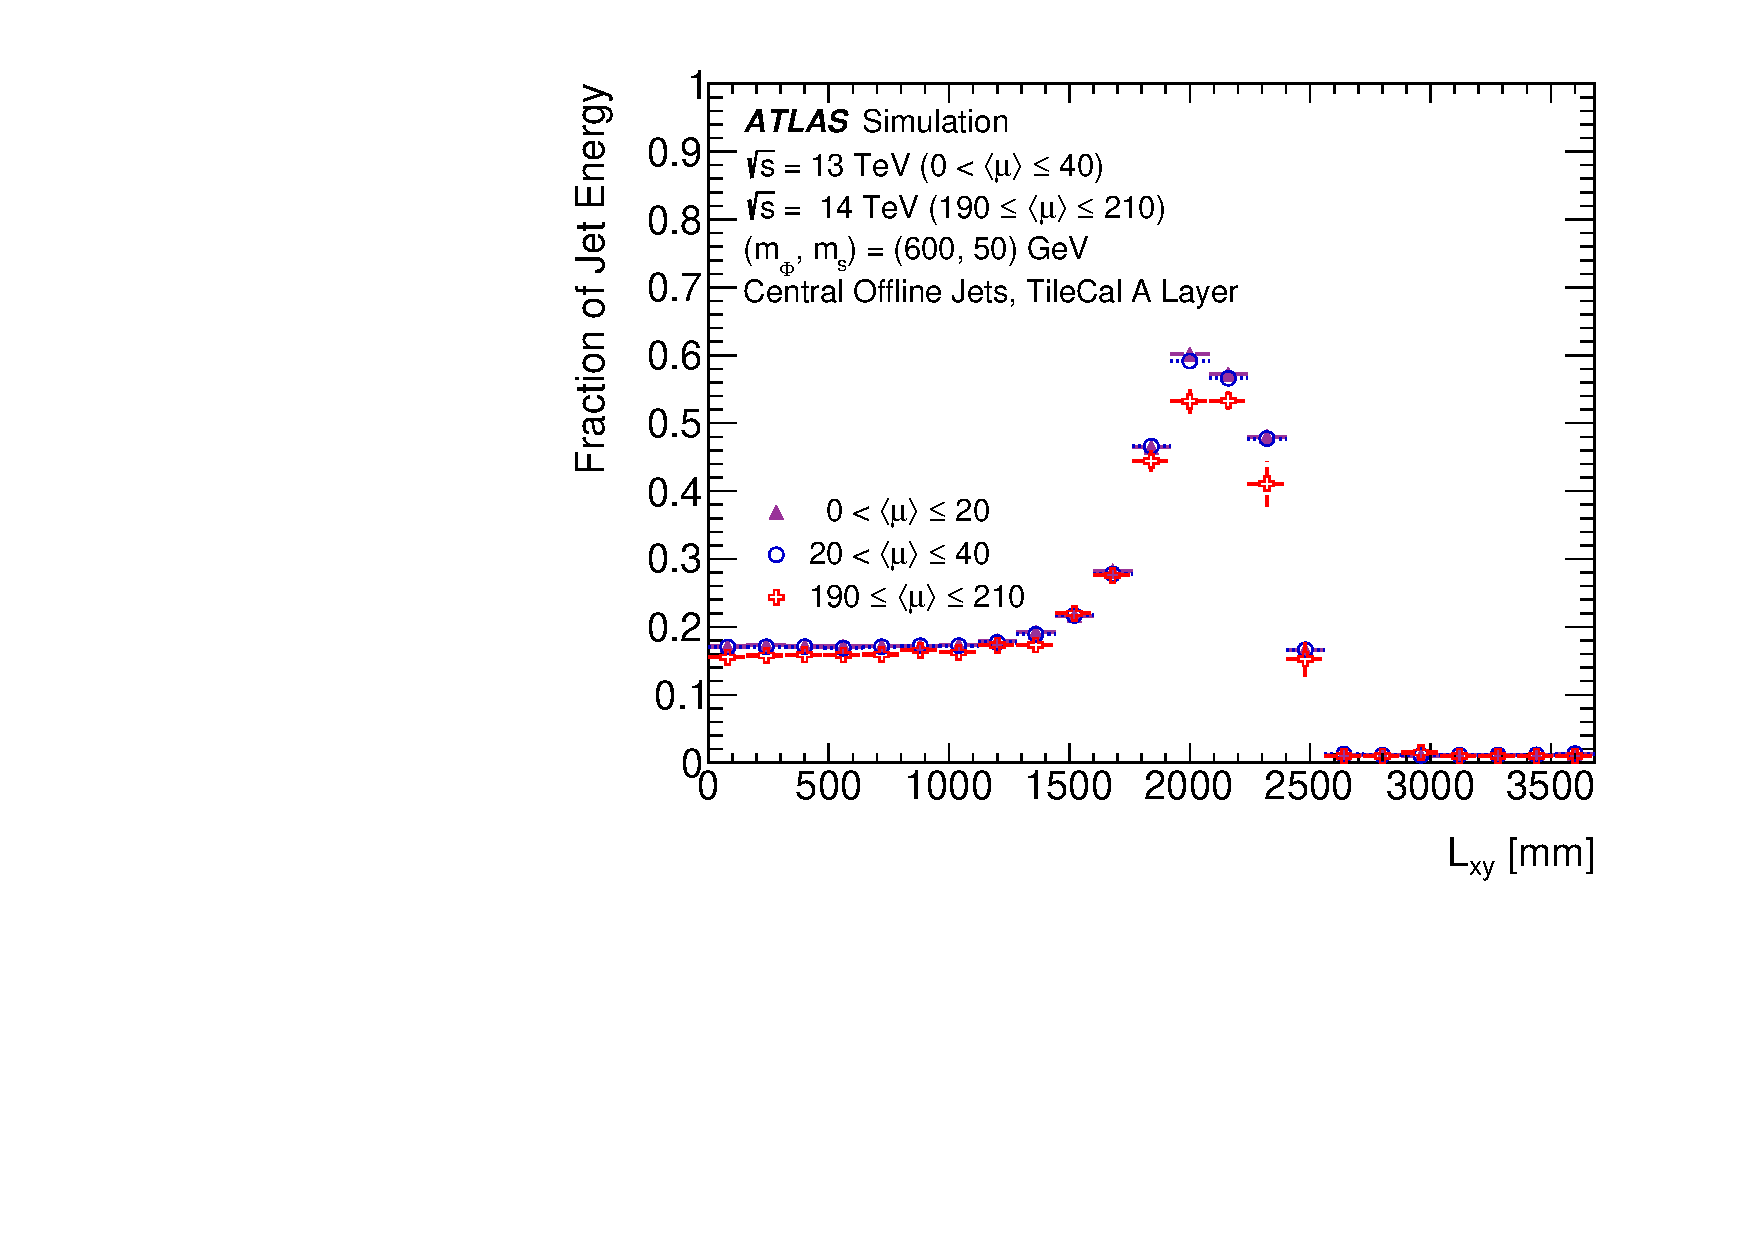
\includegraphics[width=0.47\textwidth]{figures/caloratio3.pdf}
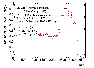
\includegraphics[width=0.47\textwidth]{figures/caloratio4.pdf}\\
\caption{Simulation projections of the sensitivity of the ATLAS experiment upgrade plans to neutral LLPs. Top: the fraction of the jet energy deposited in the A-layer (left) and BC-layers (right) of the ATLAS tile calorimeter as a function of the transverse decay position of the LLP in events with a 125~GeV Higgs-like boson decaying to two 40~GeV LLPs. Bottom: the same for events with a 600~GeV Higgs-like boson decaying to two 50~GeV LLPs.}
\label{fig:Caloratio}
\end{center}
\end{figure}


\subsubsection{Disappearing Tracks}

In the ATLAS experiment, the planned ITk upgrade of the tracking volume for the HL-LHC can be exploited to improve the existing searches for BSM particles with a disappearing track~\cite{Collaboration:2285585}.

Such particles are predicted by many well-motivated supersymmetric models such as anomaly-mediated SUSY-breaking scenarios, where the supersymmetric partners of the Standard Model $W$ bosons, the wino fermions, are the lightest SUSY state. In such models, the lightest neutralino and chargino can be nearly mass-degenerate, with a mass splitting around 160~MeV, and the chargino is consequently long lived. The combination of long lifetime and boost when produced in a high-energy collider allows the chargino
to leave multiple hits in the traversed tracking layers before decaying. When performing searches for such signatures in ATLAS, selected events are typically required to contain at least one short track, hereafter called a tracklet. To study how such searches can be improved with the ITk upgrade, some assumptions have been made for simulating events and projected detector response. The detector response is parametrised by using response functions based on studies performed with Geant4 simulations of the upgraded detector in high-luminosity pile-up conditions.

The tracklet reconstruction efficiency for signal charginos as a function of the decay radius inside the detector is shown in Figure~\ref{fig:ATLAS_DT1}. A 30\% systematic uncertainty on the background yields is assumed, as observed for the Run 2 analysis. The expected background is largely dominated by fake tracklets due to random crossings.
%
\begin{figure}[t]\begin{center}
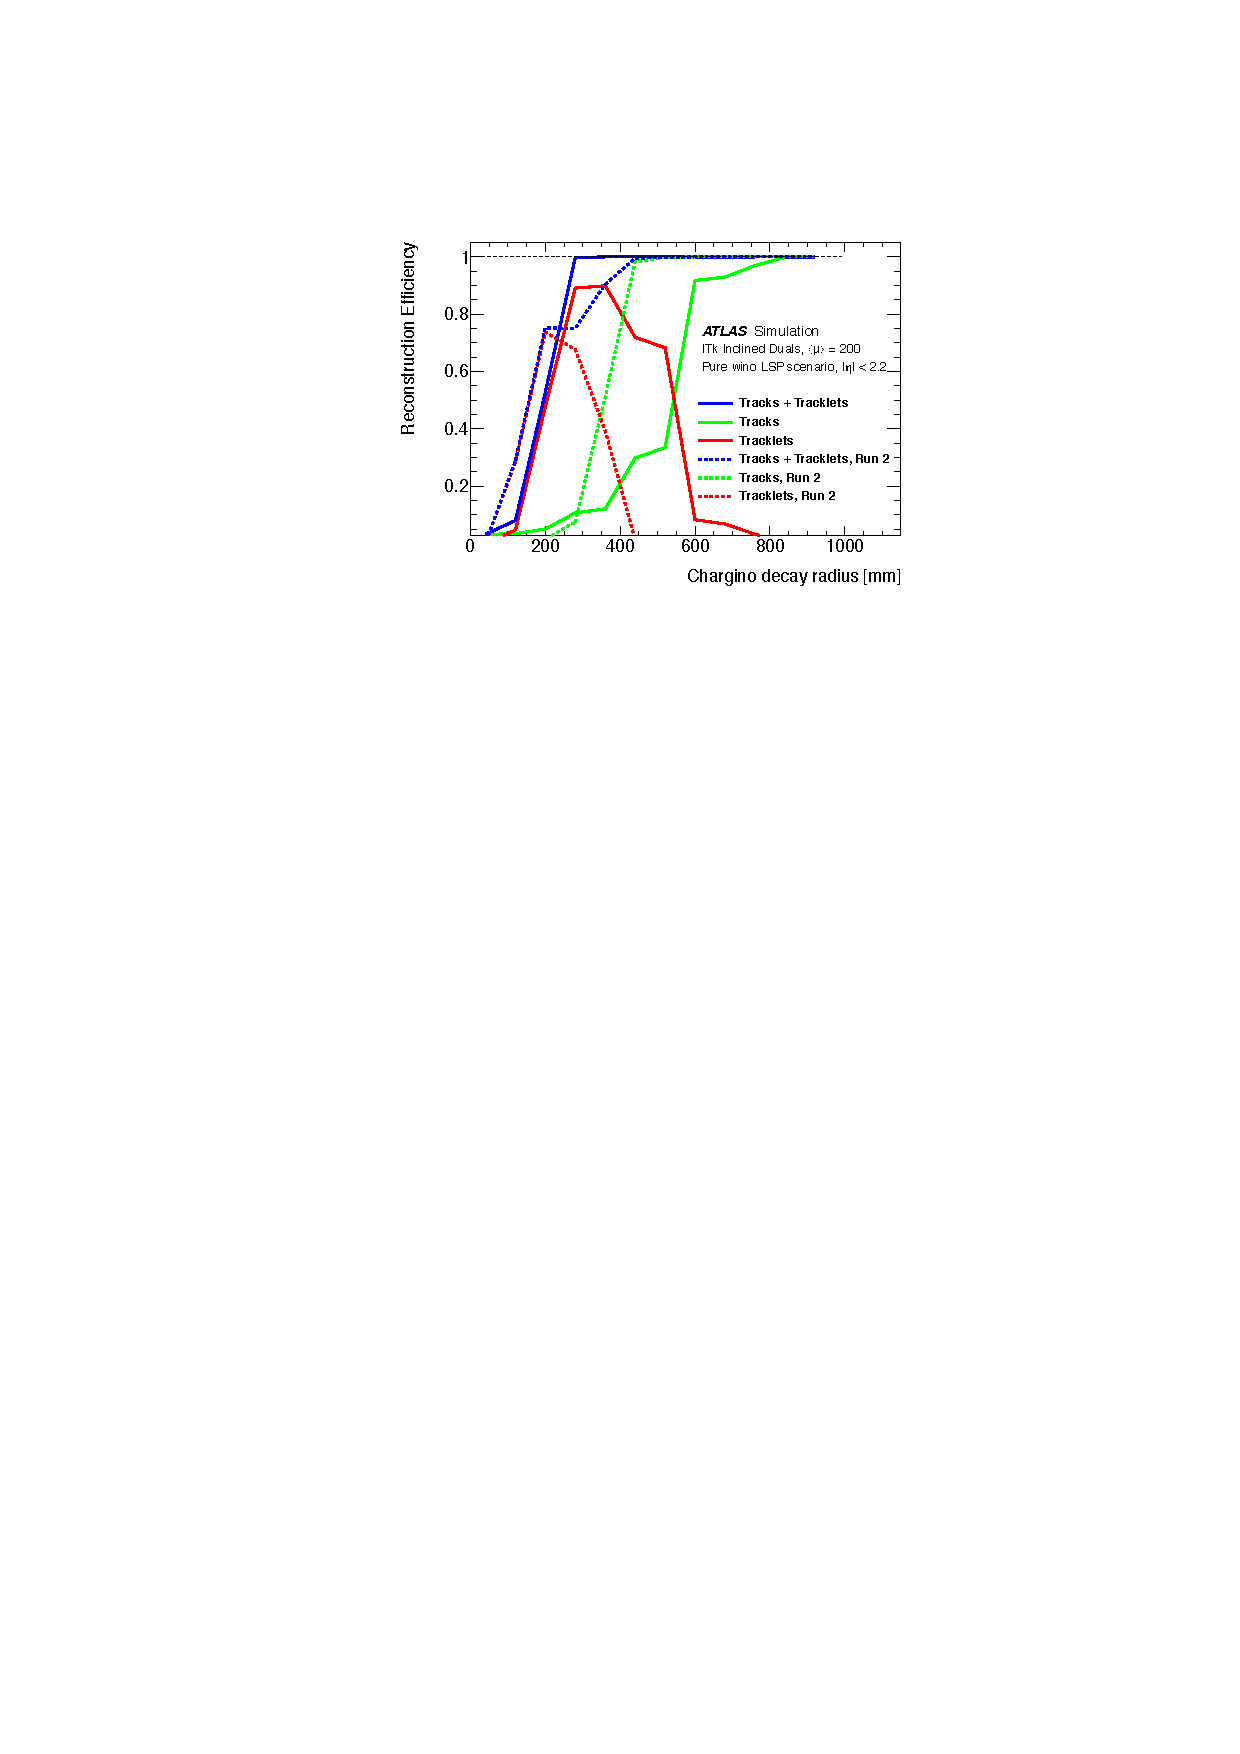
\includegraphics[width=0.9\textwidth]{figures/atlas-tdr-030-fig3-39.pdf}
\caption{ Reconstruction efficiency of the disappearing chargino as a function of decay radius using two track reconstruction techniques:~``tracklets'' refers to the short tracks mentioned in the text, while ``tracks'' refers to standard track reconstruction. The corresponding reconstruction efficiencies for Run 2 are also shown~\cite{Collaboration:2285585}.}
\label{fig:ATLAS_DT1}
\end{center}
\end{figure}

Expected limits at 95\% C.L. are shown in Figure~\ref{fig:ATLAS_DT2} as a function of the chargino mass and lifetime for a pure wino and a pure higgsino LSP scenario. For comparison, the current Run 2 limit for 36.1 ${\rm fb}^{-1}$ in the wino LSP scenario is also shown. The HL-LHC dataset of 3000 ${\rm fb}^{-1}$ extends the sensitivity of neutrinos and charginos up to 250~GeV, assuming a pure higgsino scenario.

%
\begin{figure}[t]\begin{center}
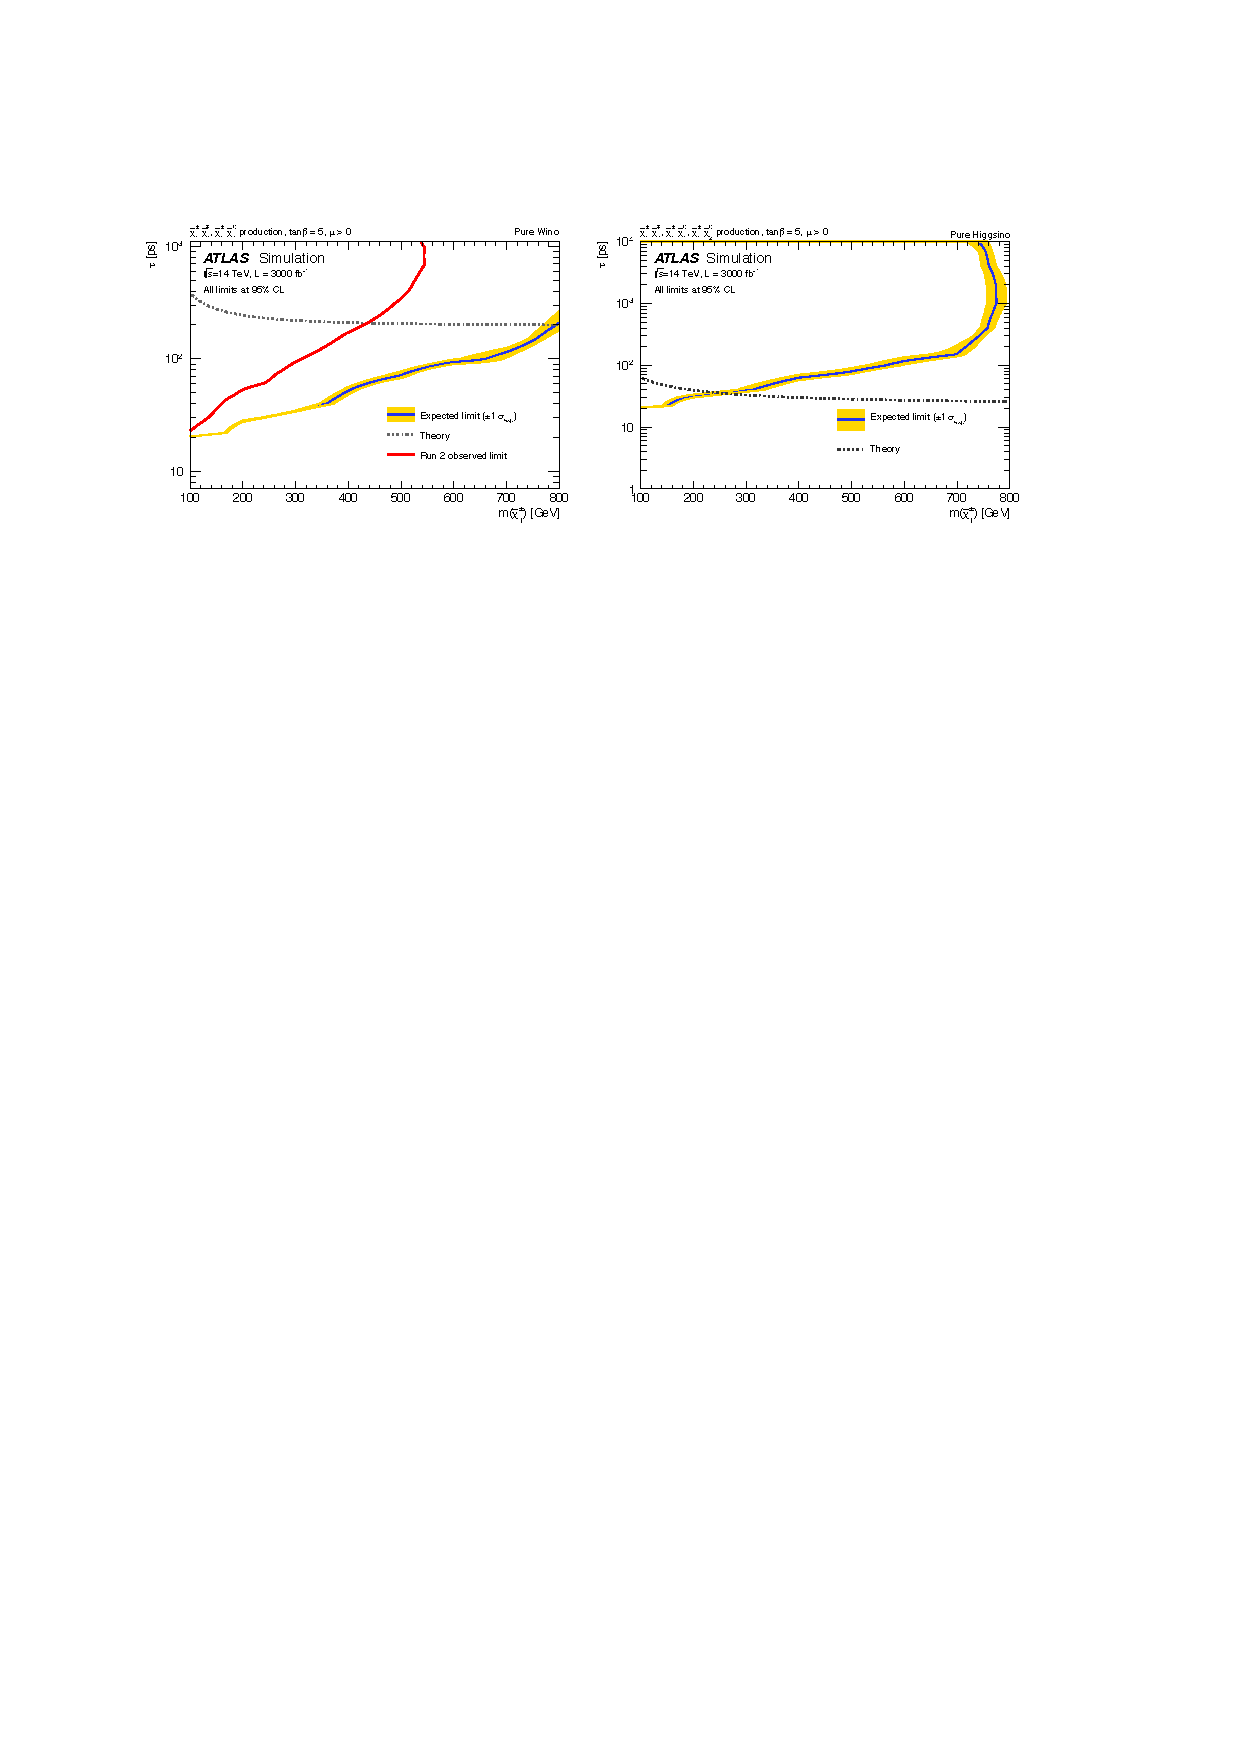
\includegraphics[width=0.9\textwidth]{figures/atlas-tdr-030-fig3-40.pdf}
\caption{Projected 95\% C.L. limits on a degenerate chargino-neutralino scenario assuming the chargino is a (left) pure wino; (right) pure neutralino. The limits include both pair production $\tilde\chi_1^+\tilde\chi_1^-$ and associated production $\tilde\chi_1^\pm\tilde\chi_1^0$ (the Higgsino model also includes the $\tilde\chi_1^\pm\tilde\chi_2^0$ mode)~\cite{Collaboration:2285585}. }
\label{fig:ATLAS_DT2}
\end{center}
\end{figure}

\subsubsection{Displaced Vertices in ATLAS}

Massive, long-lived particles with lifetimes of the order of O(10) ps to O(10) ns can decay inside the inner tracker into charged and stable particles. The products of these decays are reconstructed as tracks with measurably distant impact parameters with respect to the IP. The reconstruction of such displaced tracks is very challenging compared to the track reconstruction of prompt particles, due to fewer hits along the track and a larger parameter phase space for track finding. In order to identify a displaced vertex, one must first identify the tracks from the decaying LLP.

Several physics models predict the existence of long-lived, massive particles. For example, a standard SUSY scenario can contain a gluino with a mass of 2~TeV and a lifetime of 1~ns. The long-lived gluino hadronises into an $R$-hadron, which then decays into a 100~GeV neutralino and hadrons.

In ATLAS, this topology has been investigated in Run 2 by using a dedicated algorithm for reconstructing displaced vertices~\cite{ATL-PHYS-PUB-2017-014}. The performance expected to be achieved for the ITk upgrade for this signal has been tested with a simplified simulation which has a description of the ITk active sensors and a modeling of the magnetic field. The kinematics and location of the decay products of the R-hadron are injected into the simulation and their trajectories are extrapolated through the detector model. The probability of producing at least seven silicon hits in the ITk geometry is shown in Figure~{fig:atlas-tdr-030-fig3-41} for a 2 TeV $R$-hadron with $\tau=1$ ns. The increased volume and number of ITk layers leads to improved efficiency for the reconstruction of tracks from displaced vertices (and hence the vertices themselves) out to radial distances of up to 550 mm. The increased number of silicon layers also gives more room to veto tracks with missing hits, further suppressing backgrounds.
%
\begin{figure}[t]\begin{center}
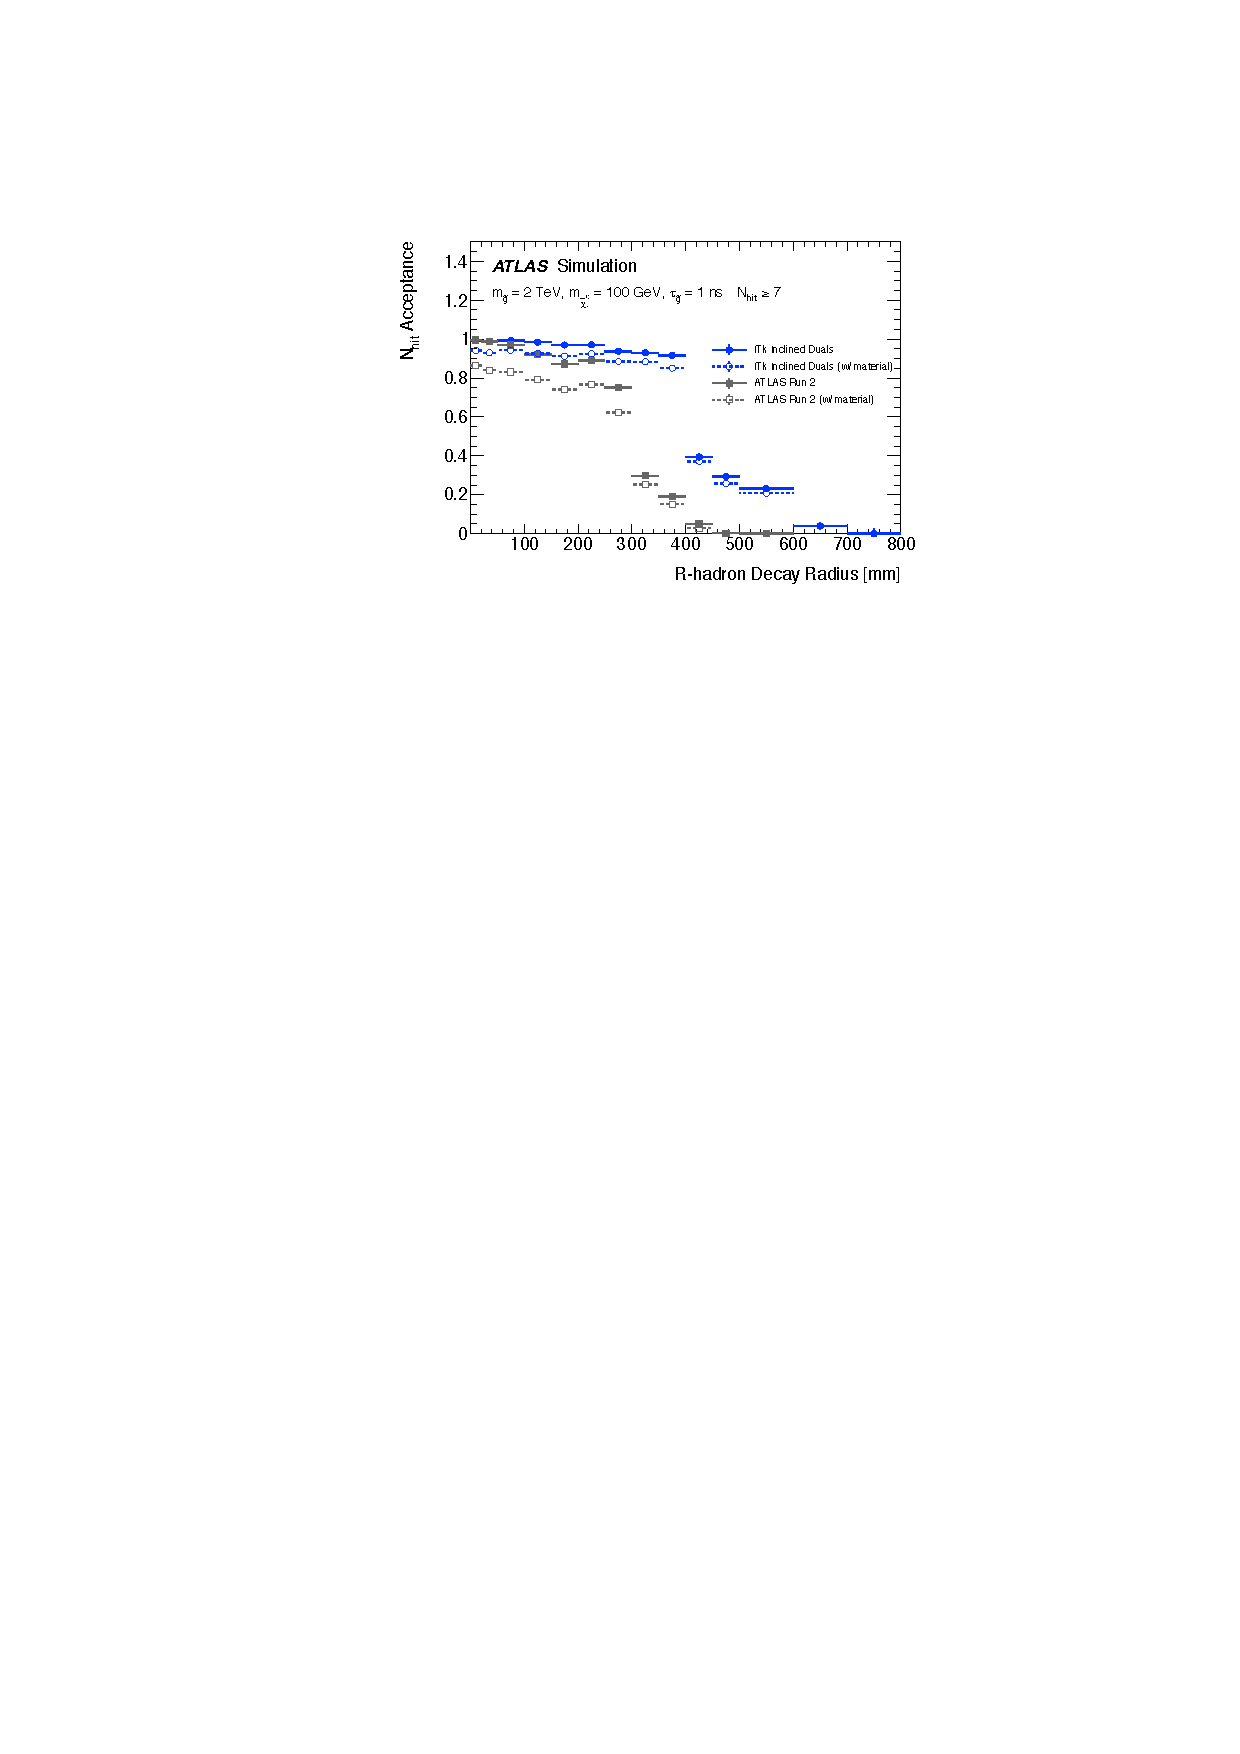
\includegraphics[width=0.9\textwidth]{figures/atlas-tdr-030-fig3-41.pdf}
\caption{Probability that tracks with $\pt>1$ GeV will traverse at least seven silicon ITk layers if they are produced in the decay of an $R$-hadron with mass 2 TeV and $\tau=1$ ns. The probability is also shown for at least seven hits with the  Run 2 layout~\cite{Collaboration:2285585}. }
\label{fig:atlas-tdr-030-fig3-41}
\end{center}
\end{figure}

\subsubsection{LLP Searches with Precision Timing at CMS}

The CMS MTD will provide new, powerful information in searches for long-lived particles. In addition to the aforementioned displaced photon search, the additional timing information can be used to provide full kinematic reconstruction of LLP decays, and can be a powerful tool in background suppression.

\paragraph{Possible Improvements in the Ability to Reconstruct LLP Mass}

A precision MIP timing detector allows each reconstructed vertex to be assigned a time and therefore to measure the time of flight of LLPs between primary and secondary vertices. Using the measured displacement between primary and secondary vertices in space and time, the velocity of an LLP in the laboratory frame, $\vec{\beta}_{LAB}^{p}$ (or, equivalently, the boost $\gamma^p$), can be measured. In such scenarios, the LLP can decay to fully visible or partially invisible systems. Using the measured energy and momentum of the visible portion of the decay, one can calculate its energy in the LLP rest frame and reconstruct the mass of the LLP, assuming that the mass of the invisible system is known.

This capability can be demonstrated in scenarios where the LLP decay produces a $Z$ boson, which then decays to an electron-positron pair. For example, in the GMSB model where the $\tilde{\chi}_0^1$ couples to the gravitino $\tilde{G}$ via higher-dimension operators sensitive to the SUSY breaking scale, the $\tilde{\chi}_0^1$ may have a long lifetime, and can be produced in top-squark pair production with $\tilde{t}\to t+\tilde{\chi}_0^1$, $\tilde{\chi}_0^1 \to Z+\tilde{G}$, $Z\to ee$.

Studies with simulated event samples have been performed to estimate the possible improved sensitivity of the search with the CMS MTD upgrade. The events are generated with Pythia 8, and the masses of the top-squark and neutralino are set to 1000~GeV and 700~GeV, respectively. Generator-level quantities are smeared according to the expected experimental resolutions. A position resolution of $12\,\,\mu\mathrm{m}$ in each of the three spatial directions is assumed for the primary vertex. The secondary vertex position for the electron-positron pair is reconstructed assuming $30\,\,\mu\mathrm{m}$ position resolution in the transverse direction. The momentum resolution for electrons is assumed to be $2\%$. Finally, the time resolution of charged tracks at the displaced vertex is assumed to be 30~ps.

The mass of the LLP is reconstructed assuming that the gravitino is massless. The fraction of events with separation between primary and secondary vertices exceeding 3$\sigma$ in both space and time as a function of the MTD resolution is shown in Figure~\ref{fig:cmsupgrade_mtd} (left). The mass resolution, defined as half of the shortest mass interval that contains $68\%$ of events with 3$\sigma$ displacement is shown in Figure~\ref{fig:cmsupgrade_mtd} (right), as a function of the MTD resolution.

\begin{figure}[t]\begin{center}
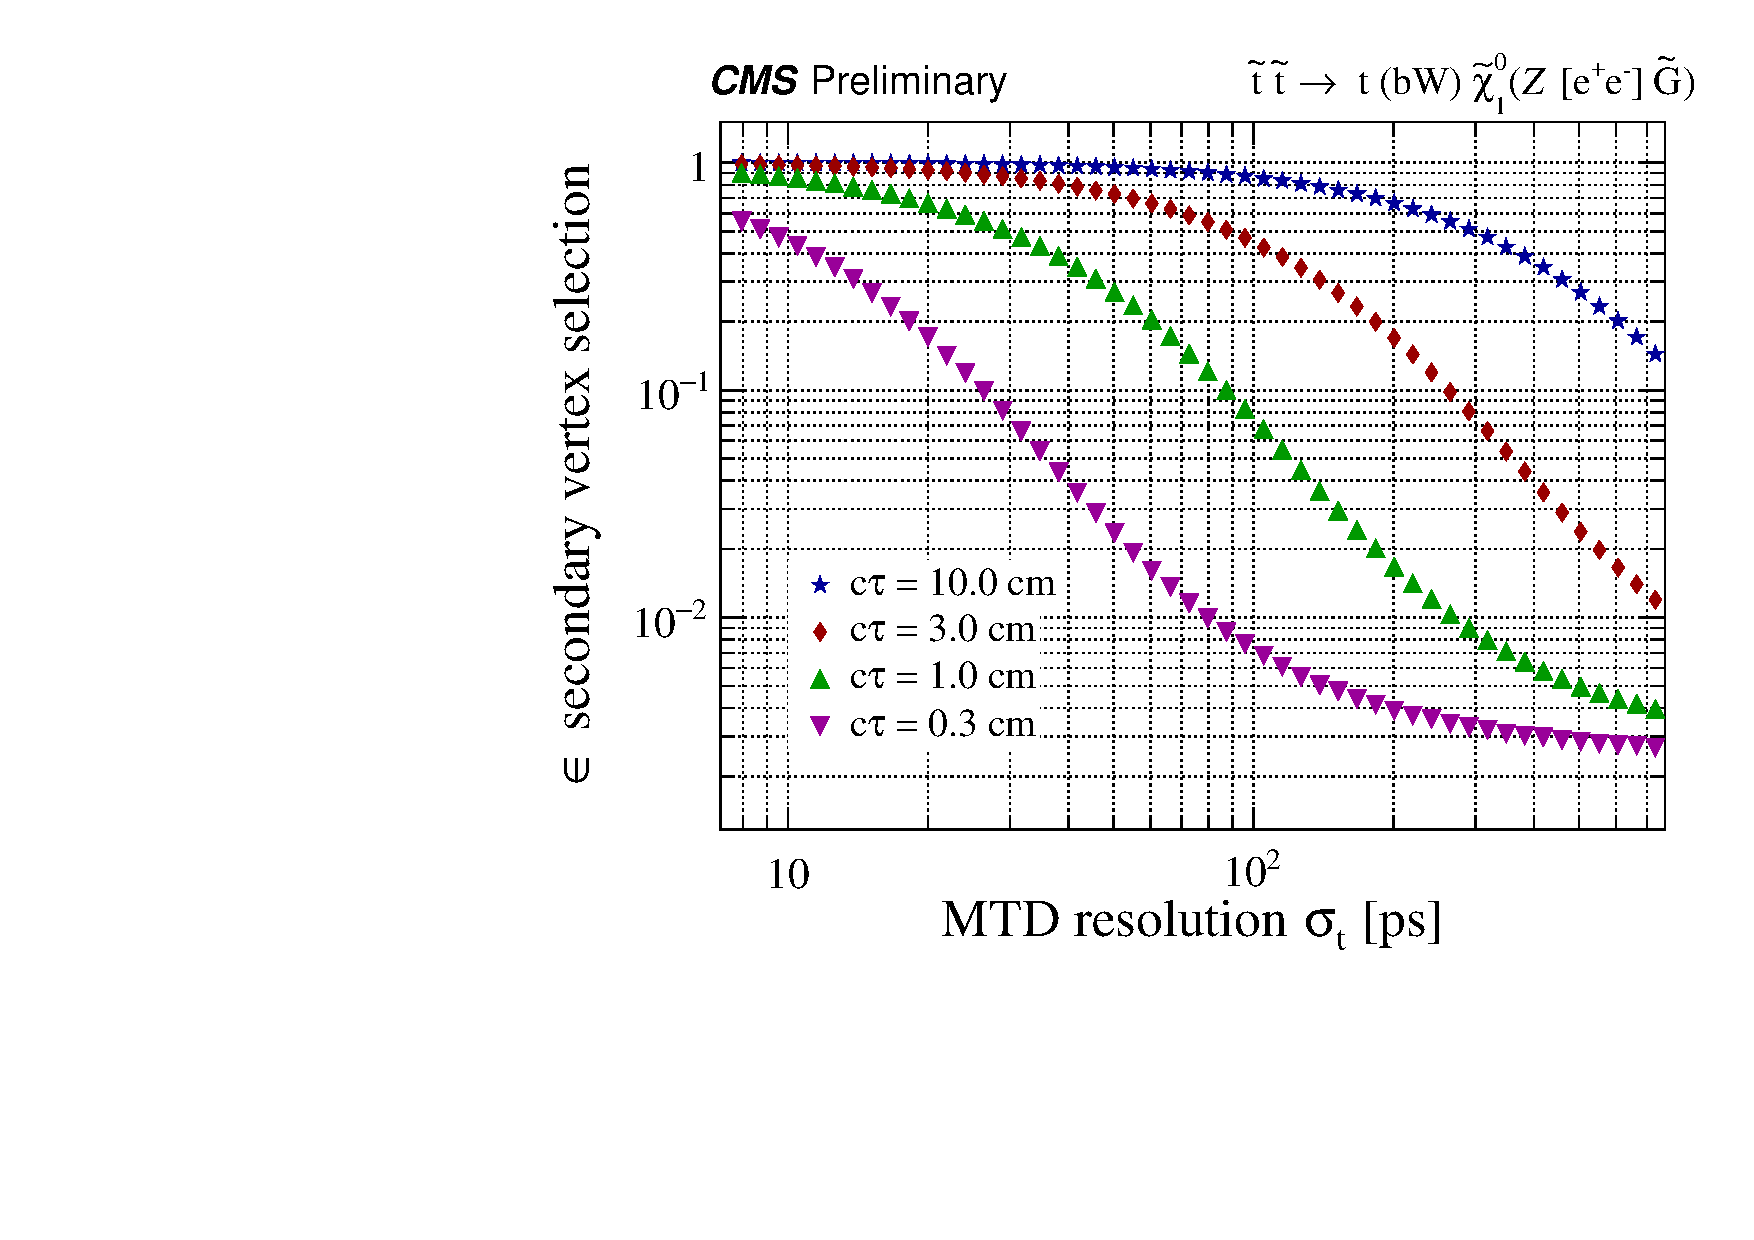
\includegraphics[width=0.47\textwidth]{figures/MTD/171025_52.pdf}
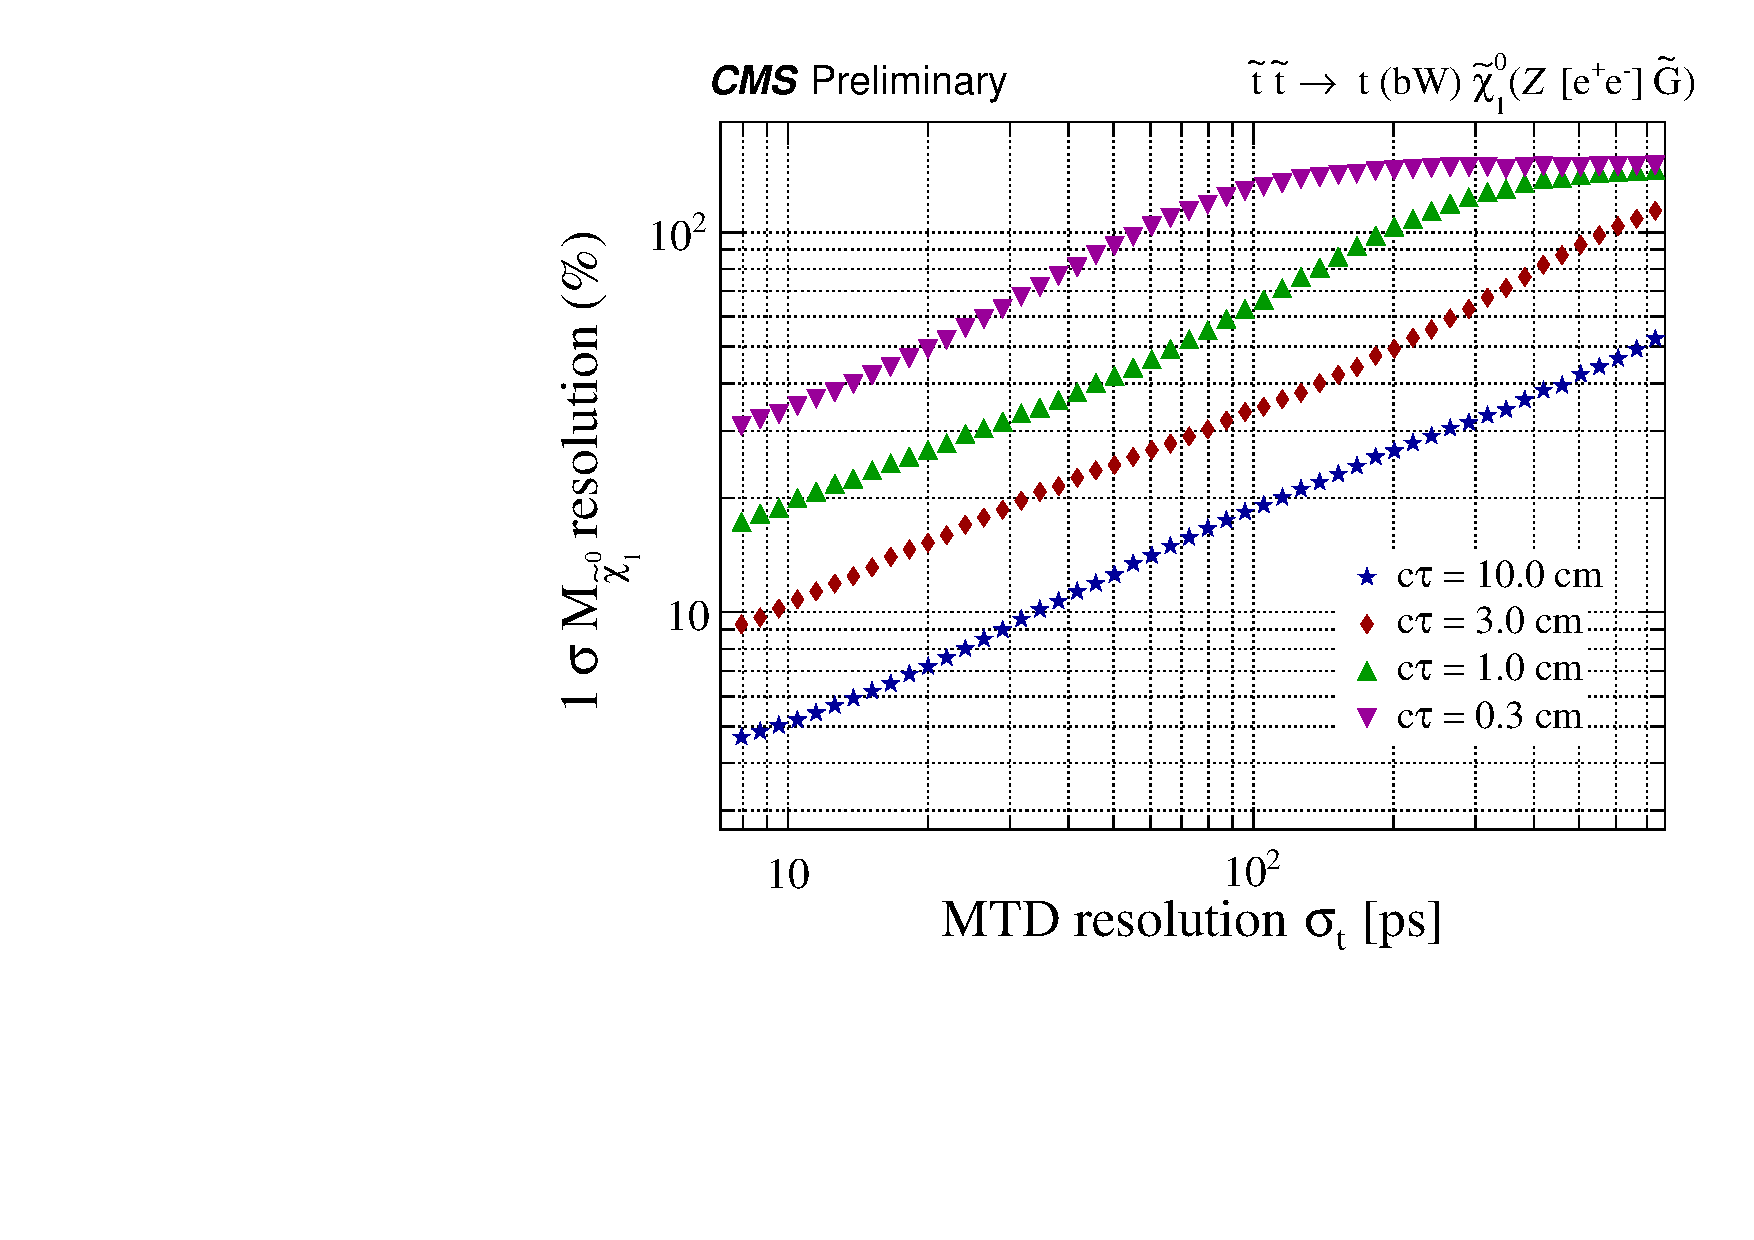
\includegraphics[width=0.47\textwidth]{figures/MTD/171025_53.pdf}
\caption{
Efficiency (left) and mass resolution (right) as a function of the timing resolution of the MTD for reconstruction of the $\tilde{\chi}_0^1$ mass in the SUSY GMSB example of $\tilde{\chi}_0^1 \to \tilde{G} e^{+} e^{-}$, with mass of $\tilde{\chi}_0^1=700$~GeV, considering events with a separation of primary and secondary vertices by more than $3\sigma$ in both space and time~\cite{MTD_TP}.
}
\label{fig:cmsupgrade_mtd}
\end{center}
\end{figure}

A similar study has been performed with another SUSY scenario where the two lightest neutralinos and light chargino are Higgsino-like. The light charginos and neutralinos are nearly mass degenerate and may become long-lived as a consequence of the heavy higgsinos. In both studies, the additional timing information from the MTD facilitates the reconstruction of the LLP mass, the resolution and efficiency of which are further improved with the excellent timing resolution of the MTD.

\begin{figure}[t]\begin{center}
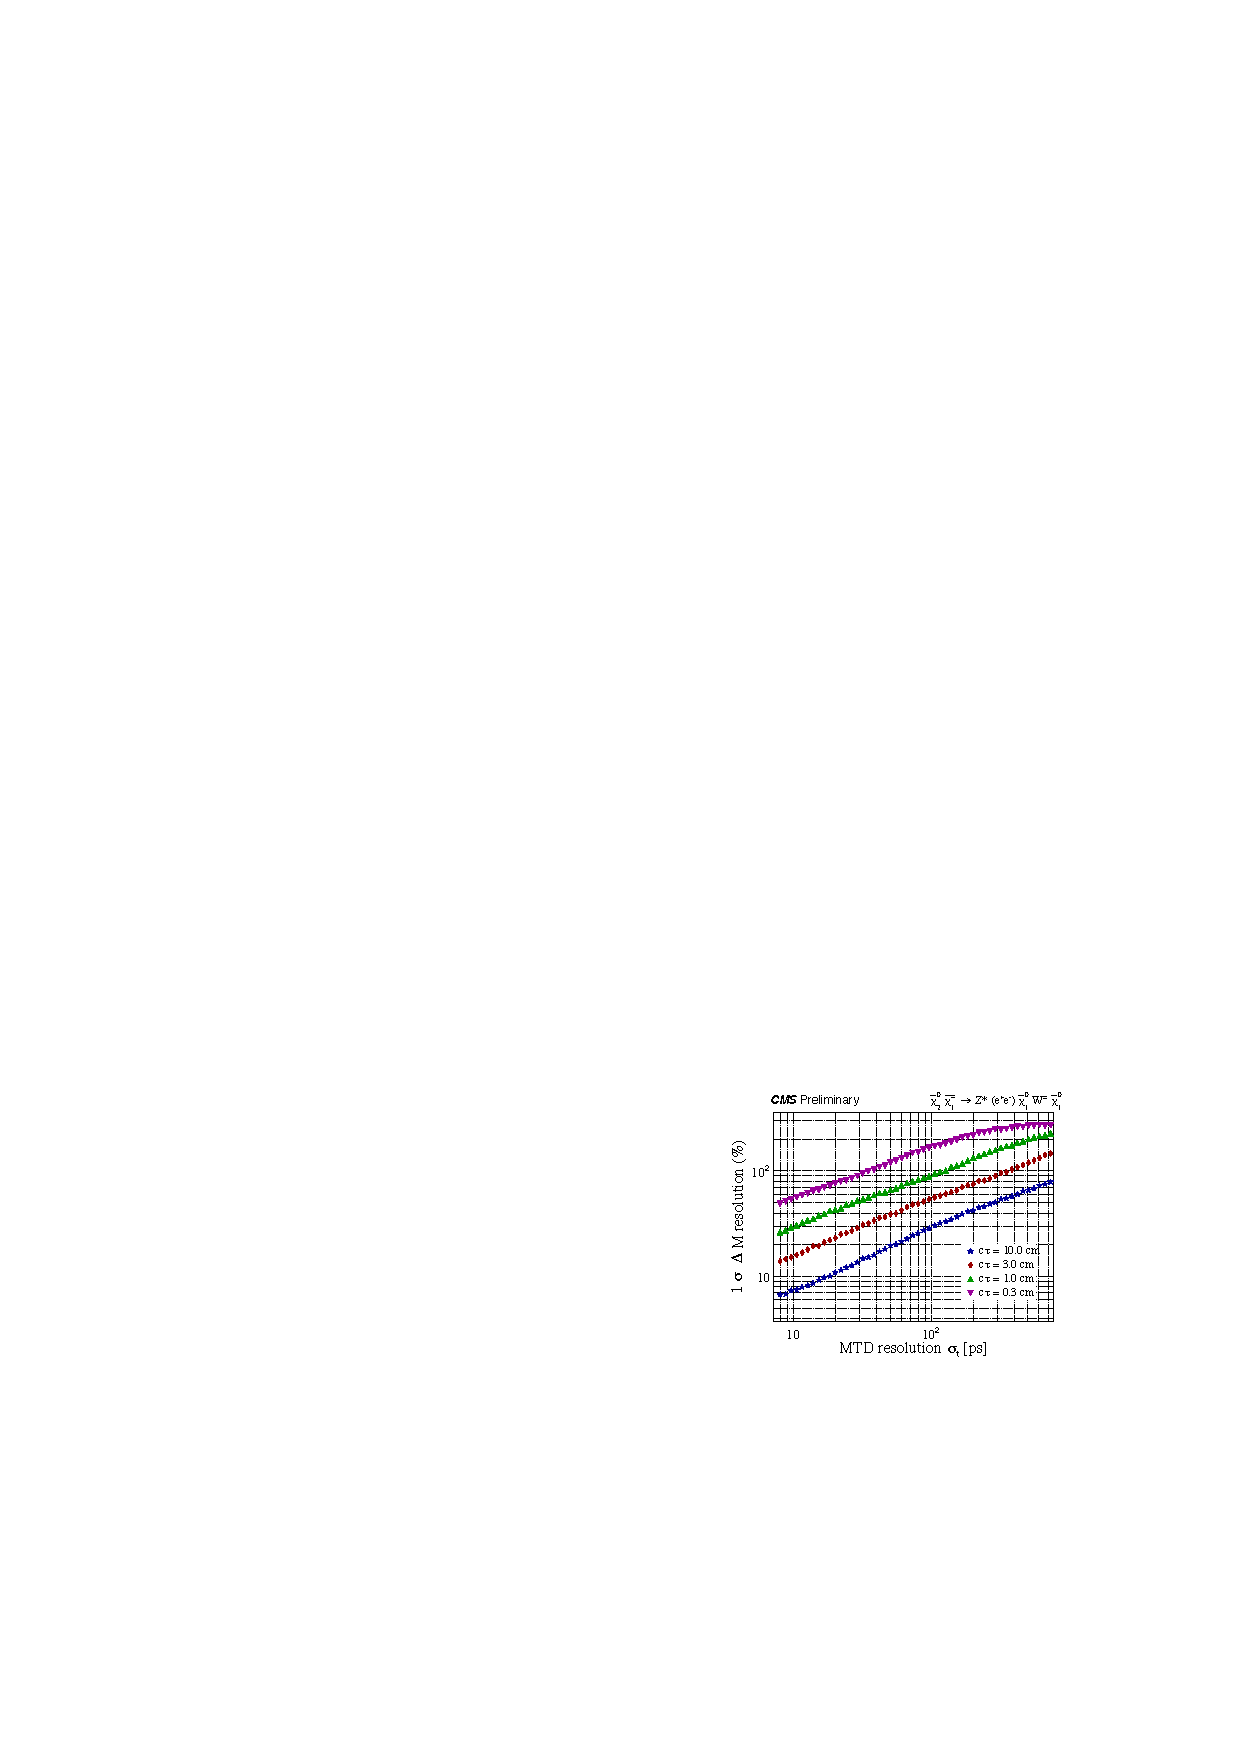
\includegraphics[width=0.7\textwidth]{figures/cms-tdr-mip-fig3-16.pdf}
\caption{
Resolution for the reconstruction of the LLP mass in the Higgsino scenario outlined in this section. The LLP mass resolution is shown as a function of lifetime and the MTD resolution~\cite{MTD_TP}.
}
\label{fig:cmsupgrade_mtd}
\end{center}
\end{figure}

%\noindent {\bf \textcolor{red}{[JB: Can we add a brief, unambiguous statement about whether the upgrade will provide improvement?]}}


\paragraph{Possible Improvement to LLPs Searches in General Using Timing Information}

Precision timing at CMS will provide a new tool to suppress the background and enhance the reach for LLPs in the HL-LHC era.
\begin{figure}[htb]
    \centering
    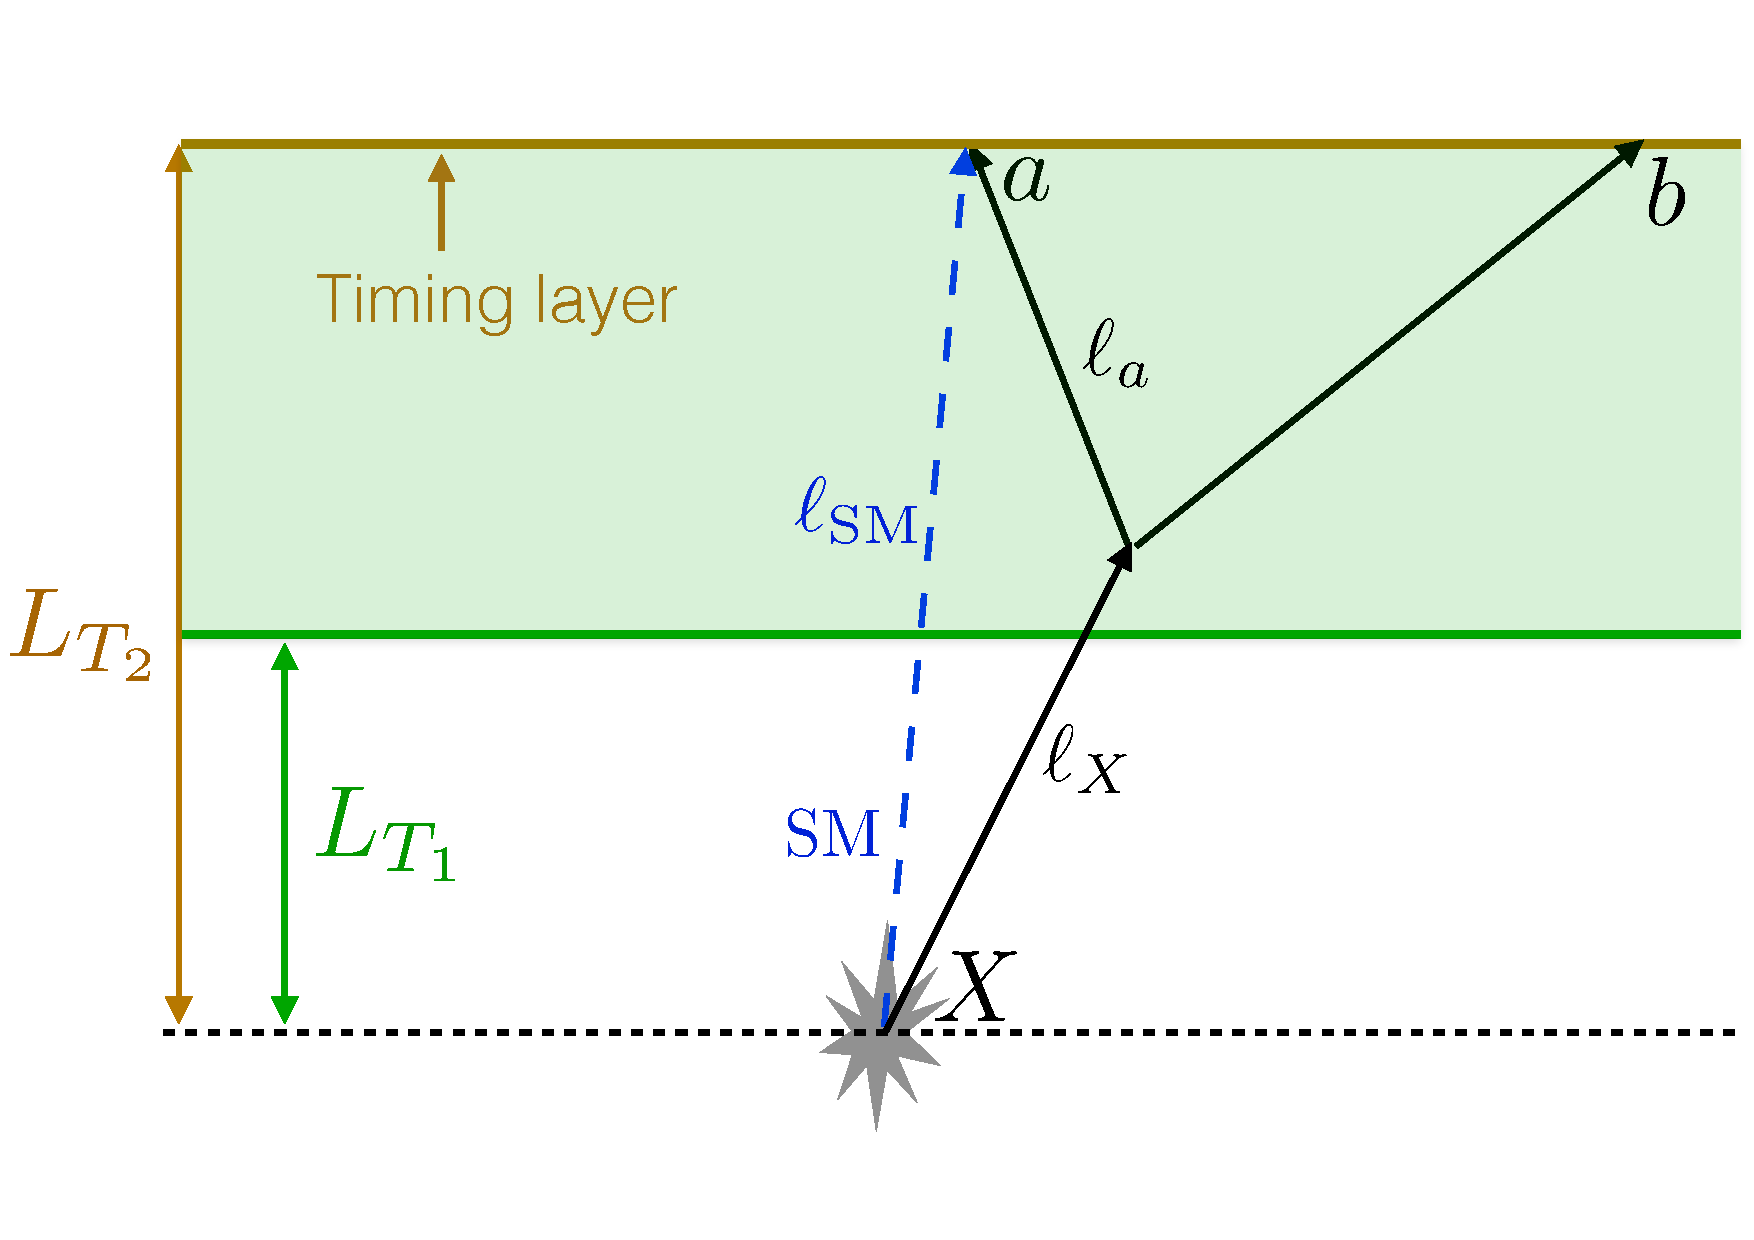
\includegraphics[width=0.9\columnwidth]{figures/MTD/schematic_drawing.pdf}
    \caption{An event topology with an LLP $X$ decaying to two light SM particles $a$ and $b$. A timing layer, at a transverse distance $L_{T_2}$ away from the beam axis (horizontal gray dotted line), is placed at the end of the detector volume (shaded region). The trajectory of a potential SM background particle is also shown (blue dashed line). The gray polygon indicates the primary vertex. Taken from Ref.~\cite{Liu:2018wte}.}
    \label{fig:drawing}
\end{figure}

A schematic of a typical signal event containing an LLP is shown in Figure~\ref{fig:drawing}. An LLP, denoted as $X$, travels a distance $\ell_X$ into a detector volume and decays into two light SM particles $a$ and $b$, which then reach a timing layer at a transverse distance $L_{T_2}$ away from the beam axis. In a typical hard collision, the SM particles generally travel very close to the speed of light. Hence, the decay products of $X$ (using particle $a$ as an example) arrives at the timing layer with a time delay of
\beq
 \Delta t = \frac{\ell_X}{\beta_X} + \frac{\ell_a}{\beta_a} - \frac{\ell_{\rm SM}}{\beta_{\rm SM}},
\label{eq:delaysimple}
\eeq
with $\beta_a \simeq \beta_{\rm SM} \simeq 1$. An ISR jet could easily be present for all processes, and can be used to ``timestamp'', i.e., to derive the time of the hard collision at the primary vertex.

For the CMS MTD located just outside the tracker volume, ${\ell_{\rm SM}}/{\beta_{\rm SM}}$ is about $O(1\,\,\mathrm{ns})$. As a result, with tens of picosecond (ps) timing resolution, a sensitivity to percent-level time delay caused by slow LLP motion, e.g., $1-\beta_X>0.01$ with boost factor $\gamma<7$, is expected to be achieved.

A theory study has been done in Ref.~\cite{Liu:2018wte} examining potential gains in sensitivity for hadronic displaced vertex reconstruction using timing information. A new trigger strategy for a delayed jet is studied by comparing the prompt jet with $\pt > 30$~GeV that reconstructs the four-dimensional primary vertex (PV4d) with the arrival time of another jet at the timing layer. The delayed and displaced jet signal, after requiring a minimal decay transverse distance of 0.2~m ($L_{T_1}$), will typically not have good tracks associated with it. Consequently, the major SM background is from trackless jets. The origins of this background can be classified into two categories: hard collision from a same vertex (SV), and pile-up (PU) from different vertices. Other types of background such as cosmic rays, beam halo, etc., can become important after the successful removal of hard collision background using various reconstruction and timing delay cuts. They are typically soft or have distinctive features to veto on; for more details see Ref.~\cite{Liu:2018wte}.

The jet faking a displaced signal, behaving as a trackless jet, has an intrinsic time delay $\Delta t=0$. However, due to the limited timing resolution in reconstructing the PV4d, it can have a time spread. The background differential distribution with respect to apparent delay time ($\Delta t$) can be estimated as
\beq
\frac {\partial N_{\rm bkg}(t)^{\rm SV}} {\partial \Delta t }= N_{\rm bkg}^{\rm SV}
\mathcal{P} (\Delta t;\delta_t^{\rm SV}).
\label{eq:bkgSV}
\eeq
The time delay cut on $\Delta t$ reduces such a background through a very small factor of $\mathcal{P}(\Delta t;\delta_t^{\rm SV})$ for large $\Delta t/\delta^{\rm SV}_t$, where $\delta^{\rm SV}_t$ is the timing resolution for the SV background, dominant by the timing detector resolution.
The LLP signal pays a much smaller penalty factor than the background due to its intrinsic delay.

The background from the pile-up requires the coincidence of a triggered hard event and objects from a pile-up (hard) collision whose PV4d fails to be reconstructed and that can mimic a signal. The differential background from pile-up can be estimated as
\beq
\frac {\partial N^{\rm PU}_{\rm bkg}(\Delta t)} {\partial \Delta t} \simeq N_{\rm bkg}^{\rm PU}
{\mathcal P}(\Delta t;\delta_t^{\rm PU}).
\label{eq:bkgPU}
\eeq
Similar to Eq.~\ref{eq:bkgSV}, $\delta^{\rm PU}_t$ is the timing resolution for the PU background, dominated by the beam spread. The key difference between the background from the pile-up and the background from the same hard collision is that the typical time spread is determined by the beam property for the former, and by the timing resolution for the latter. They typically differ by a factor of a few, e.g., 190~ps versus 30~ps for CMS with the current upgrade plan.


Using this estimation, a sensitivity projection is presented with an example signal of a Higgs boson decaying to LLPs with the subsequent decay of the LLPs into $b \bar b$ pairs, with only minimal requirements of one low-$\pt$ ISR jet, with $p_{\rm T,j} > 30$~GeV and $|\eta_j| < 2.5$, and at least one LLP decay inside the detector. Timing information is used to suppress backgrounds. The $95\%$ C.L. sensitivity is shown in Figure~\ref{fig:ctaulimitHiggs}. The decay branching ratio of the LLP $X \to j j$ is assumed to be $100\%$. The projection with $30$~ps timing resolution of the CMS MTD is plotted with thick dashed lines. Compared to other 13 TeV HL-LHC projections (with $3 ~\text{ab}^{-1}$ of integrated luminosity) without the timing information (shown in thinner, dotted and dashed lines), it is suggested that the addition of a timing cut, under the set of assumptions described above, greatly reduces background and improves sensitivity. The possibility of such a significant improvement is enticing; this projection is determined from theoretical studies~\cite{Liu:2018wte}, however, and it remains to be seen whether it is possible to realize these gains in the experiment. For example, the low threshold of the single jet would require timing information at early levels of the trigger, and out-of-time backgrounds could also reduce the gains from timing information. Nevertheless, this high-level theory analysis provides an inspiration to the experimental collaborations to perform more detailed, internal studies that will ultimately determine how realistic the projections are.

In general, the prospect of improvements in LLP searches at the HL-LHC due to precision timing upgrades for CMS (and ATLAS) remains understudied, and deserves more comprehensive experimental and phenomenological studies, including understanding and reducing out-of-time backgrounds.


\begin{figure}[ht]
    \centering
    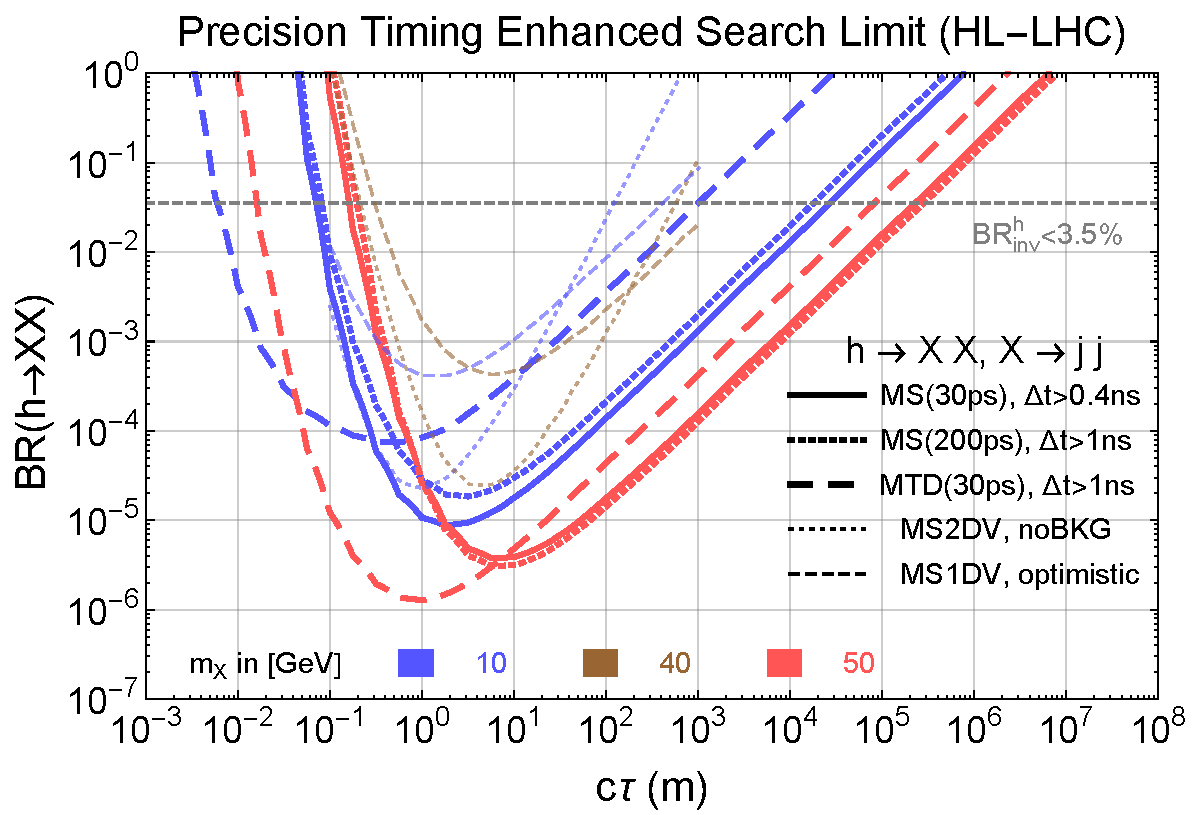
\includegraphics[width=1.0\columnwidth]{figures/MTD/10-20-50-MC-Lcalc-BRlimit-with-deltaT-cut-MS-1ns.pdf}
    \caption{Theory projection from Ref.~\cite{Liu:2018wte} of the $95\%$ C.L. limit on $\text{BR}(h \to XX)$, where $X$ is an LLP, for the production of $pp \to j h$ with the subsequent decay of $h\to X X$ and $X \to j j$ subject to assumptions in the text (one ISR jet with $p_{\rm T,j}>30$ GeV and $|\eta_j|<2.5$, and at least one LLP inside the detector). Different colors indicate different masses of the particle $X$. The thick, long-dashed lines indicate searches with the CMS MTD plus the timing requirements. The thick solid and dotted lines indicate searches with a hypothetical timing layer outside the ATLAS muon spectrometer plus timing requirements. The numbers in parentheses are the assumed timing resolutions. This provides motivation to see whether these gains can be realized by studies from within the collaborations.}
    \label{fig:ctaulimitHiggs}
\end{figure}

\subsubsection{LLP Searches with a Level-1 Track Trigger in CMS}

As discussed in Section~\ref{sec:upgrademachine}, a central feature of the CMS upgrade at the HL-LHC will be a new silicon outer tracker which allows track reconstruction for every LHC bunch crossing (at a rate of 40~MHz). The $\pt$ selection for stubs (hit pairs in the $\pt$ modules of the outer tracker) to be read out is determined by the bandwidth from the detector to the back end electronics, and is fixed at about 2~GeV. On the other hand, the choice of track finding algorithm and hardware is still being finalized, and there could be significant benefits to extending the L1 track trigger capabilities to trigger on off-pointing tracks.

To illustrate the case, a simple toy simulation to study rare Higgs boson decays into new particles with lifetimes of order of a few mm has been performed~\cite{Gershtein:2017tsv}. This study considers all-hadronic final states with low $H_T$, taking SM Higgs boson decays into four jets as an example. Theoretical motivation to look for such decays is very strong; see Section~\ref{sec:motivated_theories} for a detailed discussion. In particular, there is currently
a blind spot for lifetimes of order 1 cm in searches for new long-lived scalars
in Higgs decays, i.e. \ensuremath{h \to \phi\phi}\xspace. The goal is to probe very small branching fractions of the Higgs boson, so for this study, $BR[h\rightarrow\phi\phi\rightarrow 4q] = 10^{-5}$ is assumed. For prompt decays, the background is overwhelming, but if the $\phi$ has $c\tau$ of a few mm, the offline analysis has very low backgrounds. The problem is getting such events on tape, in particular through L1. This toy study estimates how an off-pointing track reconstruction at L1 can help. To estimate the efficacy of the approach, the resulting projections are compared with the best alternatives in the absence of an off-pointing track trigger, by using associated Higgs boson production with a $W$ boson that decays leptonically to pass a lepton trigger, or considering L1 calorimeter jets with no associated prompt tracks.

%FTR-18-018

Once these positive results were obtained, a more detailed study using the full
Phase 2 simulation of the CMS detector was performed~\cite{CMS:2018qgk}.
The more mature exploration found that a plausible extension of
the L1 track trigger to tracks with an impact parameter of a few centimeters results in
dramatic gains in the trigger efficiency. The gains are even larger for additional heavy
SM-like Higgs bosons with the same decay. These results are in agreement with the toy study described above.
A few details of the mature study will be described below.

The study focuses on small or moderate decay lengths of the new particles, 1--50~mm, and assumes
that the offline selection can remove all SM backgrounds with only a moderate loss of efficiency.
While this study focuses on the specific Higgs boson decay to light scalars,
the results and the proposed triggers are relevant for a broad spectrum of new physics searches, with or without macroscopic decay lengths.

The authors propose a simple jet clustering algorithm implementable in firmware, and compare it with anti-\ensuremath{k_t}\xspace jets~\cite{Cacciari:2008gp} with a size parameter of $R = 0.3$,
as produced by \textsc{FastJet}\xspace~\cite{Cacciari:2011ma}. This simple algorithm produces a similar performance, in both L1 trigger efficiency and rate,
to the full jet clustering using the anti-\ensuremath{k_t}\xspace algorithm.


%Displaced track finding
Then, the performance of an algorithm for reconstruction of tracks with non-zero impact parameter is presented. This approach extends the baseline CMS L1 Track Trigger design to
handle tracks with non-zero impact parameter and to include the impact parameter in the track fit. This enhanced design is feasible without greatly altering the track finding approach, but will
require more FPGA computational power than the current proposal, which only considers only prompt tracks. Tracks passing the selection are clustered using the same algorithm as described above,
and clusters containing tracks with high impact parameters are flagged as displaced jets. Though the baseline design of the L1 Track Trigger currently is optimized to find prompt tracks, these
studies show that an enhanced L1 Track Trigger can extend the L1 trigger acceptance to include new BSM physics signals.

For now, the extended L1 track reconstruction is limited to the barrel region.
In order to compare the results with prompt and extended track reconstruction, one needs to make a correction for
the rapidity coverage: prompt tracks are found in $|\eta|<2.4$, while the extended track algorithm currently only
reconstructs tracks in $|\eta|<1.0$. To scale the efficiency for finding track jets to the full
$|\eta|<2.4$ range, a scale factor based on efficiency in the full $\eta$ range and the central $\eta$ range was used. The scale factor
was comparable to the increase in L1 rate.

%Results
Figure \ref{fig:reff_dispextra} shows the expected trigger rate as a function of efficiency for the SM and the heavy SM-like Higgs bosons.

\begin{figure}[hbtp]
  \centering
    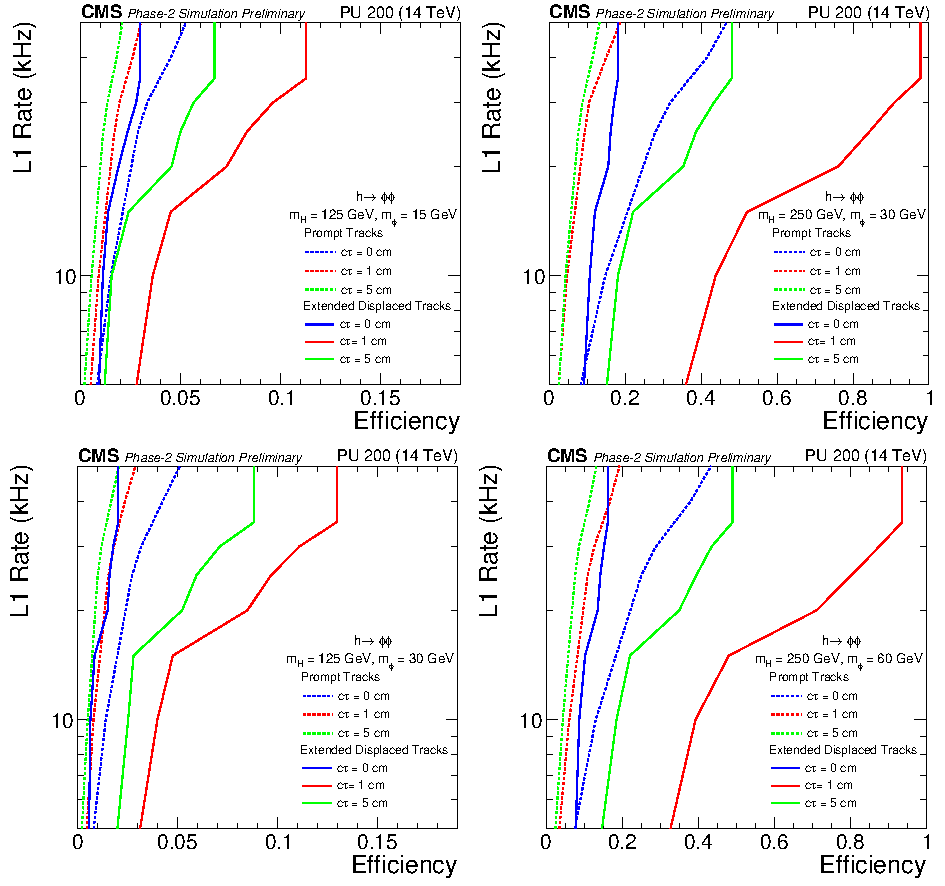
\includegraphics{tex/figures/CMS-PAS-FTR-18-018_Figure_008.pdf}
    \caption{The rate of the track jet $H_T$ trigger as a function of signal efficiency using extended track finding for the SM Higgs (left) and the heavy SM-like Higgs (right). The extended track finding performance is extrapolated to the full outer tracker acceptance as described in the text and in Ref.~\cite{CMS:2018qgk}.}
    \label{fig:reff_dispextra}
\end{figure}

The available bandwith for the triggers described above, if implemented, will be decided as a part of the full trigger menu optimization.
Here, two cases are considered: 5 and 25~kHz. The expected event yield for triggers using extended and prompt tracking are shown in Figure\,\ref{fig:money},
assuming branching fraction $\mathcal{B}[\ensuremath{h \to \phi\phi}\xspace] = 10^{-5}$ for the SM Higgs boson.
For the heavy Higgs boson, the expected number of produced signal events is set to be the same as for the SM Higgs by requiring
$\sigma_{pp \to h(250)} \mathcal{B}[\ensuremath{\Phi \to \phi \phi}\xspace] = 10^{-5} \sigma_{pp \to h(125)}$.

\begin{figure}[hbtp]
  \centering
    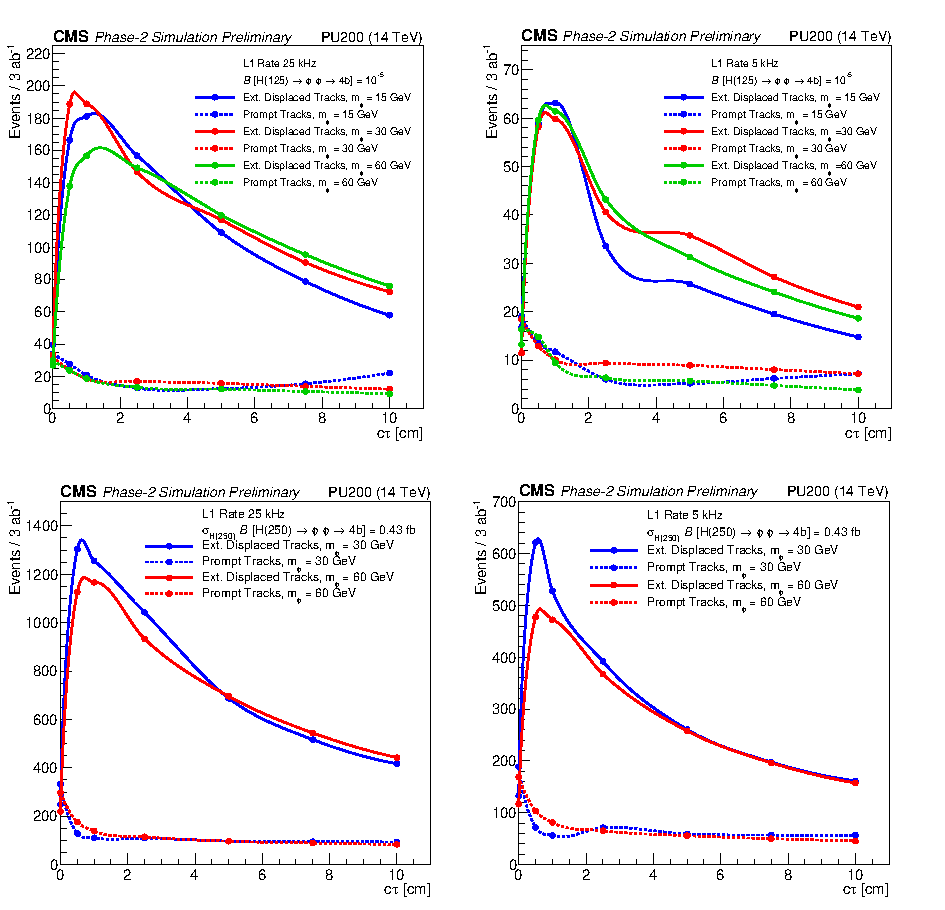
\includegraphics{tex/figures/CMS-PAS-FTR-18-018_Figure_009.pdf}
    \caption{This plot shows the number of triggered Higgs events (assuming ${\mathcal{B}[\ensuremath{h \to \phi\phi}\xspace] = 10^{-5}}$, corresponding to 1700 events) as a function of $c\tau$ for two choices for the trigger rates: 25~kHz (left), 5~kHz (right). Two triggers are compared: one based on prompt track finding (dotted lines) and another that is based on extended track finding with a displaced jet tag (solid lines)~\cite{CMS:2018qgk}.}
    \label{fig:money}
\end{figure}

For the exotic Higgs decays considered, given the total Phase 2 dataset of 3 inverse attobarns and branching fraction of $10^{-5}$,
CMS would collect $\mathcal{O}(10)$ events, which should be sufficient for discovery.
A plausible extension of the L1 track finder was considered, to select tracks with impact parameters of a few cm.
That approach improves the yield by more than an order of magnitude. The gains for the extended L1 track finding
are even larger for the events with larger $H_T$, as demonstrated by the simulations of heavy Higgs boson decays.

\subsection{Open Questions and New Ideas}\label{sec:upgradeideas}


The higher data rate and more powerful machinery in the high-luminosity era bring new prospects to LLP searches. Searches that are too challenging for the current machine may become feasible with the HL-LHC upgrades, and it is important to explore such possibilities to the full extent. Existing search methods, triggering, and reconstruction algorithms should also be updated to take full advantage of the new hardware capabilities. As the upgrade scope is being defined and finalized in the near future, it is of particular importance to evaluate the physics cases, which will also motivate the upgrade and inform its designs.

\subsubsection{New Studies for the HL-LHC}

In Section~\ref{sec:upgradesearch}, various analyses with displaced signatures are presented in the context of how detector and trigger upgrades at the ATLAS and CMS experiments for the HL-LHC can improve their sensitivity. As was shown in Section~\ref{sec:upgrademachine}, while the upgrades for both experiments differ in detail, they are similar in concept and scope. It is therefore important to perform the same LLP search projections for both experiments to compare performance and evaluate the complementarity of the two experiments.

For example, both experiments explore the idea of a fast timing detector at HL-LHC. The CMS MTD aims for full-coverage of a barrel layer plus endcap disks, while the ATLAS HGTD plans for multiple layers of endcaps. How the different $\eta$ coverage of the timing layer might impact LLP searches will be an interesting question to answer. In the case of calorimetry, the ATLAS LAr electromagnetic calorimeter is segmented in $z$, providing the additional pointing capability to find displaced photons. On the other hand, the CMS ECAL electronics upgrade in the barrel, and HGCAL upgrade in the endcaps, will considerably improve its timing resolution to identify photons that are out-of-time. A sensitivity comparison of both experiments will provide helpful information in understanding photon reconstruction and the combined reach of both experiments.

In addition, there are other developments that the experiments could take advantage of, especially in the context of LLP searches in Run 3 or at the HL-LHC. One such development is the ability to perform an analysis using physics objects at the trigger level, rather than their more complex, offline counterparts. This analysis method, which has been pioneered in a 8~TeV search for dijets with CMS~\cite{Khachatryan:2016ecr}, is called data scouting. Data scouting could be used, for example, to reduce the $\pt$ thresholds of jets and muons used in dark photon or hidden particle searches. Another example of how it could be used for a LLP search is by allowing changes in the L1 muon patterns in order to trigger on non-pointing muons.

Another development that could be exploited for future LLP searches is machine learning. Machine learning could be used in particle identification, reconstruction, or generation, not to mention in the LLP analysis or reinterpretation.

Furthermore, as new models are being proposed and new channels open up in the realm of LLP searches, many with final states challenging for the current detector conditions, it is important to evaluate their sensitivities in the high luminosity era. Here are a few of such interesting searches that are on the agenda.

\begin{itemize}
\item \textbf{Inelastic dark matter}

While stringent limits are currently placed on WIMP-type dark matter from direct detection, indirect detection, and collider searches, dark matter particles can exist in a hidden sector with additional particles and forces. A representative example of a hidden sector consists of a dark matter particle which is charged under a hidden gauge or global symmetry. The DM can have both a symmetry-preserving mass and, if the symmetry is spontaneously broken, also a symmetry-violating mass, which splits the mass eigenstates. This inelastic dark matter (iDM) scenario~\cite{TuckerSmith:2001hy,Bai:2011jg,Izaguirre:2015zva} consists of two DM states that couple only off-diagonally to one another. Such iDM can be probed at colliders with the production of $\mathrm{DM}+\mathrm{DM}^*$ (where $\mathrm{DM}^*$ denotes the heavier DM state) in association with a hard SM object $X$, followed by the subsequent decay of $\mathrm{DM^*}\rightarrow\mathrm{DM} +Y$ for some potentially different SM states $Y$. The production is summarized as
\begin{eqnarray} \label{eq:schematic-production}
pp  &\to&   X +  \mathrm{DM}+\mathrm{DM}^*   \nonumber \\     &\to&  X + \mathrm{DM}+ \biggl( \mathrm{DM}^* \to \mathrm{DM}+  { Y}\biggr)     \equiv  X + \slashed{E}_{\rm T}+ Y ~,~ \nonumber
\end{eqnarray}
where $X$ is any state that can be used to trigger on the event and reconstruct $\slashed{E}_{\rm T}$, such as an ISR jet, and $Y$ depends on the mode by which DM couples inelastically to the SM.

One concrete, representative version of such models can be realized when the mediator is a dark photon and $Y$ is a pair of leptons. The weak coupling between the SM and the hidden sector suggest the heavy eigenstate is meta-stable, creating a displaced signature. Because the mass splitting is small between the two eigenstates, the lepton pair is also typically softer compared with GMSB models, with $\pt$ values of a few to tens of GeV for a $O(10\,\,\mathrm{GeV})$ DM. The displaced muon trigger and reconstruction strategy with the muon system upgrade at CMS can likely improve searches for this scenario. The soft $\pt$ spectrum in this case particularly motivates the lowering of the $\pt$ threshold in the displaced muon trigger turn-on. Moreover, the additional timing information from the fast-timing detector opens up the possibility of reconstructing the mass splitting, while taking advantage of the good resolution of the timing detector for even low-$\pt$ particles. Sensitivity studies for iDM with a dark photon mediator are planned for the CMS MTD upgrade. The projections will also be of value to searches for other types of dark sector models, such as self-interacting dark matter~\cite{Hochberg:2014dra}, that give rise to soft displaced lepton pairs. %{\bf \textcolor{red}{[JB: Can our ATLAS colleagues add a similar discussion about their upgrade potential here?]}}

\item \textbf{Dark showers}

If the hidden sector has a QCD-like structure with dark quarks and hidden forces, a mediator between the SM and the hidden sector, such as a $Z'$ or heavy Higgs boson, can decay into some number of dark quarks that subsequently shower and hadronize into dark mesons, some of which are meta-stable and decay back into SM particles after a macroscopic distance from the proton-proton interaction point. A showering dark sector can yield a particularly rich collider phenomenology that may give rise to a high multiplicity of displaced objects often low in $\pt$. Depending on the final state, searches for a hadronic shower with emerging~\cite{Schwaller:2015gea} or semi-visible~\cite{Cohen:2015toa} jets can be improved with the increased acceptance and enhanced resolution due to the tracker upgrades at both ATLAS and CMS, as well as the finer granularity endcap calorimeter (HGCAL) at CMS. A dark shower with displaced photon pairs can benefit from the improved timing resolution with the ECAL electronics upgrade, as well as the new timing detectors. A dark shower with displaced lepton pairs, similar to the aforementioned case of inelastic dark matter, can be probed with better sensitivity with the muon system upgrades, as well as the fast timing information. For more details on dark showers, see Chapter~\ref{sec:showers}.

\end{itemize}

{\bf \textcolor{red}{[BS: Removed last two bullet points. James, you can put them back in/expand if you want]}}


\subsubsection{New Detectors at Future Collider}

If we are only limited by our imagination, what new detectors may exist at a future collider that can open up new capabilities for LLP searches? Regardless of practical constraints, studies for such bold new proposals also help us understand our current experimental reach and optimize our search strategies.

\begin{itemize}
\item \textbf{4-dimensional tracker with timing}

Extending from the ``timing layer'' approach for HL-LHC upgrades, it is clear more time measurements on the track are favorable. In particular, the time of flight between layers is a powerful discriminant for choosing hits on a track. A future tracker that provides 4-dimensional information, including precise timing information for every layer, can significantly improve track reconstruction by reducing combinatorics, providing purer track seeds, and remove fake stubs. Assuming high-$\pt$ particles, each layer's time measurement is advanced by 30~ps and so preserves the differences in vertex times. Low $\pt$ particles will have even more discrimination power since their paths leave longer times between hits in consecutive layers of the tracker.

Major technical advances will need to happen to achieve such an implementation, including development of fine-pitch sensors with good timing resolution, improvements in scaling and power consumption, electronics upgrade, and alterations to present pattern recognition methods in track finding.

\item \textbf{Timing detector outside ATLAS Muon System}

As discussed in Section~\ref{sec:upgradesearch}, by using a prompt object, such as an ISR jet, to ``timestamp'' an event, and cutting on the timing delay from the LLP, the new timing layer (MTD) at CMS can help significantly reduce the background and improve LLP search sensitivity. The CMS MTD is located between the tracker and the ECAL with a distance to the beamline of about $1.2\,\,\mathrm{m}$. If one imagines a fast timing layer outside the ATLAS muon system (MS) with a distance of approximately $10\,\,\mathrm{m}$~\cite{Liu:2018wte}, timing information at such distances could provide additional discriminating power for particles with longer lifetimes. In Figure~\ref{fig:ctaulimitHiggs}, the projection with a $30$~ps timing resolution of such a hypothetical detector outside the ATLAS muon system is plotted in a thick solid line. A less-precise timing resolution ($150$~ps) has been also considered with a cut $\Delta t > 1$~ns to suppress background. The LLP efficiency is largely unaffected by this change, while low-mass LLPs lose sensitivity by a factor of a few.

The CMS MTD timing upgrade for the HL-LHC already provides significant improvement~\cite{Liu:2018wte}. The timing detector outside the ATLAS muon system has the notable benefits of lower background, a larger volume for the LLP to decay and more substantial time delay for the LLP signal due to longer travel distance.
%As an estimate of the best achievable sensitivity, given that the muon system is an ideal place to look for LLPs at the LHC, we have also considered a hypothetical timing layer outside of the ATLAS MS. We found robust enhanced sensitivity to LLPs at MS using the timing information.
Moreover, due to the extended time delay of the LLPs in the volume of the muon system, less-precise timing can still achieve similar physics goals.  As a result, it can serve as an estimate of the best achievable sensitivity using timing information in LLP searches.

\item \textbf{New double-sided tracking layer very close to the beamline}

Inspired by the L1 track trigger design at CMS for the HL-LHC, a scenario may be imagined where an additional tracking layer close to the beamline is added, mechanics and radiation hardness permitting. This would allow a track veto close to the IP to be implemented, and extend the LLP sensitivity to even smaller displacements. Moreover, if such a layer can be designed with double-sided modules, similar to the CMS outer tracker approach for the HL-LHC, hit pairs (stubs) from this layer can be used in a L1 track trigger for displaced tracks or disappearing tracks. The feasibility of such an approach would depend on the ability to store and process data at a rate not allowed by current technology. On the other hand, it is helpful to consider more innovative data-scouting methods at trigger level to store and select information, or introduce additional discriminating factors to reduce the rate for particular data streams, for the potential of exploring such signatures.

{\bf \textcolor{red}{[BS: Removed last two bullet points. James, you can put them back in if you want]}}

%\item \textbf{Additional layer of lead between the ATLAS calorimetry and the muon system to veto punch-through jets}

%Outcome of A. Hass, D. Curtin, and J. Beacham project at LBL workshop, summer 2018.

%\item \textbf{More blue-sky ideas}: TBA


\end{itemize}

\section{LHCb Upgrade}
\subsection{Introduction}

The LHCb experiment is designed to detect the decay of long-lived particles: beauty and charmed mesons. As so, it is naturally suited for the search of BSM long-lived particles in a range of mass and lifetime not too dissimilar. It is the only LHC experiment to be fully instrumented in the forward region $2<\eta<5$, where $B$ and $D$ decays are abundant and their decay length is enhanced thanks to the boost. In this region, detector occupancy is extremely high and therefore during LHC Run 1 and Run 2, the experiment has been run at reduced luminosity compared to ATLAS and CMS. However, an upgrade of the detector is foreseen to run at a five times larger luminosity ($2\times 10^{33}\text{cm}^{-2}\text{s}^{-1}$) in LHC Run 3 (starting in 2021) while maintaining or improving the current physics performance. This first upgrade phase (Phase-I) will entail a novel trigger paradigm where all sub-detectors are fast enough to be read out in real time and the first trigger level is done in software. This trigger scheme is  extremely flexible and offers a great opportunity for searches of striking signatures like those of BSM long-lived particles. This upgrade comes earlier than the ATLAS and CMS upgrades planned for the HL-LHC phase (starting in 2026) and will be followed by a Phase-II upgrade (planned for 2031) to run at an even more challenging luminosity of $\sim 2\times 10^{34}\text{cm}^{-2}\text{s}^{-1}$. 
%CVS: mention LHCb Consolidation phase?

Section~\ref{sec:ulhcbperf} gives a brief overview of the (Phase I) upgraded-LHCb detector-design and the expected performance of sub-detectors. 
An overview of its capabilities in the context of LLP searches is given in Section~\ref{sec:ulhcbphys} with a few example signatures. 
Finally, an overlook of the plans for the Phase-II upgrade and some thoughts on the opportunities given by putative additional detector features are reported in Section~\ref{sec:ulhcbphaseii}.



\subsection{LHCb detector and trigger upgrade for Run 3 (Phase I)}
\label{sec:ulhcbperf}

In LHC Run 3, LHCb plans to take data at an instantaneous luminosity of $2\times 10^{33}\text{cm}^{-2}\text{s}^{-1}$, a factor five higher compared to the current one. The LHCb detector needs to be upgraded to cope with the higher radiation dose and most importantly to avoid the saturation of the trigger rate and exploit the higher luminosity. The main bottleneck in the current trigger is in the first stage, which reduces the accepted rate from 30 to 1 MHz directly at hardware level. For the upgrade, the hardware trigger will be removed and the full event will be read out at the bunch crossing rate of the LHC (40~MHz), with a very flexible software-based trigger. \\

\begin{table}[h!]
    \centering
    \begin{tabular}{lrrr}
         & Current Conditions & Phase-I Conditions & Phase-II Conditions \\
        \hline
        $\cal L$ & $4 \times 10^{32} \text{cm}^{-2}\text{s}^{-1}$ & $2 \times 10^{33} \text{cm}^{-2}\text{s}^{-1}$ & $2 \times 10^{34} \text{cm}^{-2}\text{s}^{-1}$\\
        $\int_{ } \cal L$   & $8 \text{fb}^{-1}$ by 2019 & $50 \text{fb}^{-1}$ by 2030 & $300 \text{fb}^{-1}$ by 203x \\
        $\sqrt{\text{s}}$       & 13 TeV & 14 TeV & 14 TeV \\
        $\mu$    & 1.1 & 5.5 & 50 \\
        \hline
    \end{tabular}
    \caption{LHCb current and upgraded operating conditions. Instantaneous luminosity $\cal L$, integrated luminosity $\int_{ } \cal L$, $pp$ collision energy $\sqrt{s}$ and average number of visible interactions $\mu$ are listed.}
    \label{tab:cond}
\end{table}

Table \ref{tab:cond} summarises the current and upgraded conditions of the detector. To cope with the larger occupancy and higher rate of the upgraded detector, the electronics of all the sub-detectors have to be upgraded and some sub-detectors fully replaced. This is the case for the whole tracking system which plays a crucial role in LLP searches.\\

The upgraded tracking system consists of the VErtex LOcator (VELO), surrounding the interaction point, the Upstream Tracker (UT), a tracking station placed before the magnet, and the Scintillating Fibers tracker (SciFi), three stations after the magnet. 
In the VELO~\cite{LHCb-TDR-013}, the current strips will be replaced by pixel detectors, with a custom developed ASIC (VeloPix) able to withstand a maximum hit rate of 900 Mhits/s/ASIC. The UT~\cite{LHCb-TDR-015} is composed of four silicon micro-strip planes, with finer granularity and larger acceptance compared to the current tracker. Each station of the SciFi has four planes of 2.5 m long scintillating fibres read out by silicon photo-multipliers.

The upgrade components most important for LLP searches are probably the  VELO, the tracking and the software trigger. In the following subsections a brief description of their design and capabilities is given.


\subsubsection{Upgrade VELO}
The VELO plays a fundamental role in LLP searches at LHCb: together with the large boost particles usually get in the forward direction, a very precise measurement of the LLP vertex position allows LHCb to access very low lifetimes that are often not accessible at ATLAS and CMS.

In upgrade conditions, the number of tracks and primary vertices will increase by about a factor five, making it much more difficult to identify displaced vertices close to the beam-line, left alone to do it in real time.
The VELO was thus completely redesigned to cope with the new conditions, maintain high physics performance and allow real time readout for the software trigger. The new VELO has a pixel rather than strip geometry and its distance from the LHC beams is reduced from 8 to 5 mm. This allows to improve the vertex resolution (\ref{fig:ulhcb_pvres}) and to reduce the rate of unphysical (ghost) tracks.

\begin{figure}[h]
\centerline{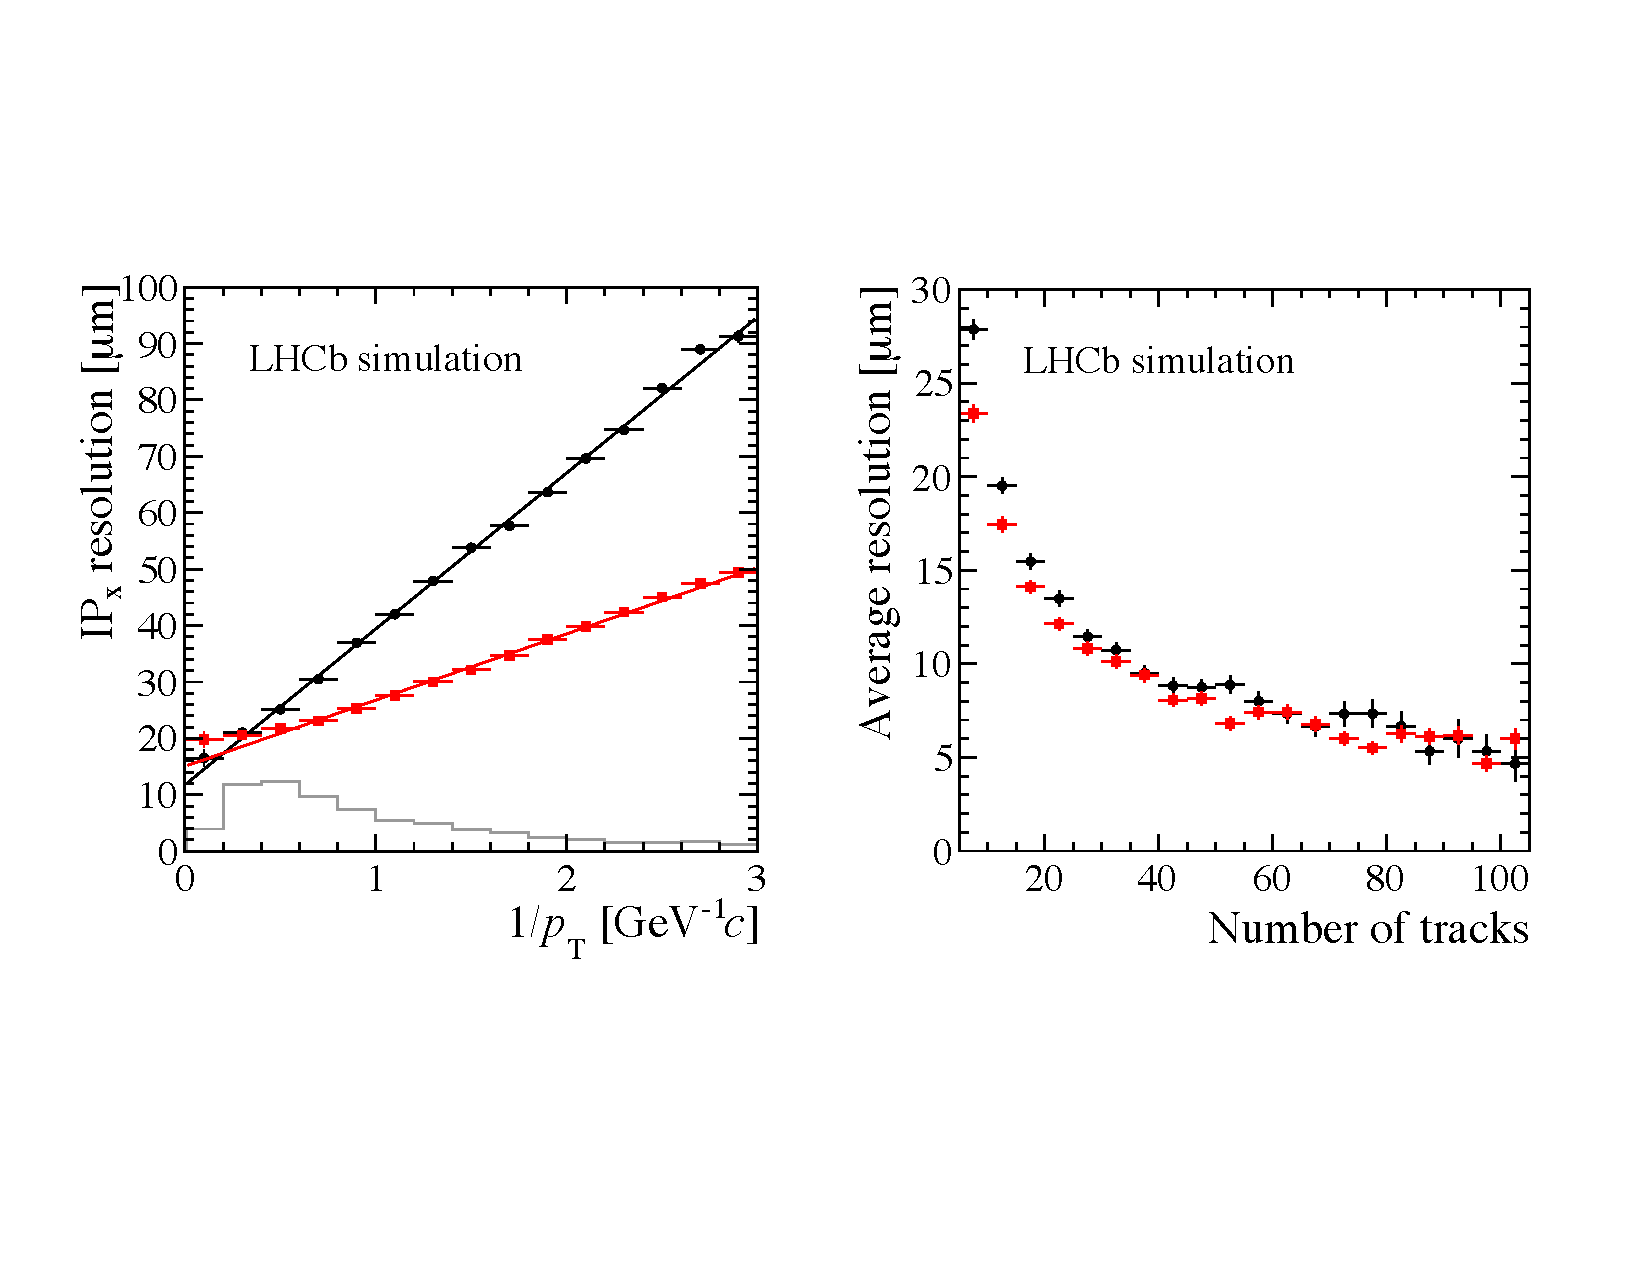
\includegraphics[width=\textwidth]{figures/lhcb_vertexres.pdf}}
  \caption{Resolution of the primary vertex as a function of number of tracks in the $x$ (left) and $z$ (right) direction. The same kind of improvement is also expected for secondary vertices (SV).}
  \label{fig:ulhcb_pvres}
\end{figure}

The pattern recognition efficiency is superior to the one of the current VELO evaluated in upgraded conditions. This can be seen for different observables. Particularly important for LLP searches is the efficiency as a function of the distance from the origin in $z$: for the upgraded VELO, the efficiency approaches $100\%$ and is uniform in a window of 20 cm around the interaction point, thanks to the new configuration of the modules in the $z$ direction and the shorter distance from the beam. After 20 cm in $z$ the VELO acceptance degrades pretty fast, making that the upper limit for LLP decay lengths with vertices reconstructible in the VELO. A display of the upgrade VELO geometry and its acceptance in both forward and backward direction is given in Figure~\ref{fig:ulhcb_veloacc}

Another important figure to evaluate the performance of the detector is the IP resolution, especially in LLP searches where it can be exploited to reduce the background due to fake tracks. With the upgrade the IP resolution significantly significantly improves for low \pt tracks. For example, the IP resolution along $x$ for tracks with \pt of 0.5\gevc is $40\mu{\rm m}$ in the upgrade versus 70 in the current VELO. 
The replacement of strips with pixel sensors also makes the pattern recognition faster for the same multiplicity. This can be used in the trigger to find tracks and identify displaced vertices in the trigger, making it possible to soften or remove inefficient $\pt$ requirements.\\

\begin{figure}[h]
  \centerline{\includegraphics[width=\textwidth]{figures/lhcb_veloperf.pdf}}
  \caption{A comparison of the current and upgrade VELO $z-$layouts is shown on the left. The top layout (black) is the current VELO while the bottom layout (red) is the upgrade VELO. On the right the track reconstruction efficiency is shown as a function of the origin in $z$ for the current (black) and upgrade (black) VELO in upgrade conditions.}
  \label{fig:eff}
\end{figure}

\begin{figure}[h]
\centerline{\includegraphics[width=\textwidth]{figures/lhcb_veloacceptance2.pdf}}
  \caption{On the left is a display of the upgrade VELO geometry and a comparison with the LHCb spectrometer acceptance which is shaded in yellow. On the right the $\eta$ acceptance of the upgrade VELO geometry is given both for forward and backward tracks. The fraction of tracks crossing three and four modules is given in red and black, respectively.}
  \label{fig:ulhcb_veloacc}
\end{figure}

Real tracks created in the VELO material can be a significant background to LLP searches (see more details in Appendix~\ref{app:background}. The total material budget of the upgrade VELO is similar to the current one (about $20\%$ radiation lengths) and is dominated by the Radio-Frequency foil separating the beam vacuum from the vacuum of the sensors.
However, the average percentage of radiation length before the first measured point is significantly reduced in the upgrade VELO, passing from $4.6\%X_0$ in the current design to $1.7\%X_0$ in the upgrade VELO.

\subsubsection{Upgraded trigger}

The online event selection in the LHCb experiment during the 2010-2018 running period is performed by a trigger composed of a hardware level (L0), and two software levels, High Level Trigger 1 (HLT1) and the High Level Trigger 2 (HLT2). The L0 reduces the rate from 30 MHz to 1 MHz, using information from the calorimeter and muon systems. Typical thresholds at the L0 are $\pt>1.4\gevc$ for muons and $E>2.5\gev$ for electrons. The software trigger performs a partial event reconstruction at HLT1, reconstructing tracks and primary vertexes for any particle down to $\pt=500\mevc$, followed by complete event reconstruction at HLT2, reducing further the rate to 12.5 kHz (in Run 2).

Given the higher istantenoeus luminosity foreseen after the Phase 1 upgrade, a new trigger system, able to fully exploit the LHC potentiality, has been designed.

The upgraded LHCb trigger consists of two paradigms, a triggerless readout and full software trigger. 
In addition, as already tested in Run 2, a real-time alignment and calibration will allow to achieve offline-quality reconstruction level already in the trigger and a higher signal purity of interesting decay channels. Figure~\ref{fig:ulhcb_trigger} shows the current and the upgrade trigger scheme. 

\paragraph{Triggerless redout and full software trigger}
With the LHCb trigger upgrade the 1 MHz readout limitation will be removed, allowing the full event rate to be processed in software. This will increase the efficiency for several final states which, already in Run 2, cannot benefit from the higher luminosity because of the L0 bottleneck. Figure~\ref{fig:triggervsLumi} shows the saturation for not muonic final state with increasing luminosity.
Moreover, a purely software trigger will not necessitate the tight $\pt$ requirements currently applied at the hardware trigger level. Thanks to this, several physics program involving low-$\pt$ particle, currently prevented because of the low L0 efficiency, will be possible.

\paragraph{Turbo stream}
Starting from Run 2, offline-quality aligment and calibration is applied between the HLT1 and the Hlt2 level. This made possible the design of a new dedicated
trigger output, called Turbo Stream. The event record is written directly from the trigger and processed by the Tesla application~\cite{Aaij:2016rxn}. Its output can be directly used for physics analysis, without the need of offline reconstruction.
Several variation to Turbo have been introduced in the last few years. For the 2015 data taking, the first version of Turbo allowed only the exclusive triggered candidate to be saved, without keeping the rest of the event and discarding all sub-detectors information. 
While the event size was an order of magnitude smaller than for full stream data, any analysis relying on additional infos from the surrounding event could not used Turbo stream data. 
For this reason, in 2016, Turbo++ was implemented, where full event reconstruction was  persisted. Finally, in  2017, a new intermediate solution between Turbo and Turbo++, called Turbo SP (Selective Persistence) was used. With Turbo SP both the trigger candidate and a subset of reconstructed event is saved. This extremely flexible solution allows the analyser to choose which objects to save, minimizing the size of the stored event. A sketch of the evolution of Turbo is showed in Figure~\ref{fig:turbo}.
In view of a full software trigger in the Upgrade, Turbo becomes the only available solution. The reduced event size, would indeed allow to store candidate at high rate, fully exploiting the improvement due to the L0 removal.  


\begin{figure}[h]
\centerline{
 \includegraphics[width=0.5\textwidth]{figures/Trigger2015.pdf}\\
\includegraphics[width=0.5\textwidth]{figures/TriggerUpgrade.pdf}	}
  \caption{Scheme of the current (left) and of the upgraded LHCb trigger scheme (right).}
  \label{fig:ulhcb_trigger}
\end{figure}

\begin{figure}[h]
\centerline{\includegraphics[width=0.6\textwidth]{figures/L0vsLumi.pdf}}
  \caption{Trigger yield as a function of the luminosity. For not muonic channels, the saturation effect due to L0 bottleneck can be observed.}
  \label{fig:triggervsLumi}
\end{figure}

\begin{figure}[h]
\centerline{\includegraphics[width=0.95\textwidth]{figures/Turbo.pdf}}
  \caption{Sketch of the evolution of Turbo.}
  \label{fig:turbo}
\end{figure}




\subsection{Upgrade LHCb projections: LLP signatures}
\label{sec:ulhcbphys}

The much higher luminosity and improved capabilities of the upgraded LHCb detector is expected to largely improve the LHCb capabilities in LLP searches in LHC Run 3. In the following, the prospects for a few LLP signatures are given to showcase the upgrade potential. However, the potential of the upgraded trigger-less readout has not been completely explored yet and its great flexibility could be exploited in several ways.

\subsubsection{Displaced di-leptons}
The upgraded LHCb experiment is expected to have exceptional sensitivity to low-mass displaced dilepton signatures thanks to mass resolution, excellent vertexing and the online selection allowed by the trigger-less readout.

The upgrade LHCb sensitivity to dileptons has been explored in the literature in the context of dark photon searches. Two complementary signatures have been considered: an inclusive search for $A'\to \mu\mu$ and a search for using radiative charm decays $D^{*0}\to D^{0}A'(ee)$.
The inclusive search~\cite{Ilten:2016tkc} scans a very large region from the dimuon threshold $2m_{\mu}$ all the way up to the $Z$ pole. The second proposed signature~\cite{Ilten:2015hya} exploits a tag of the radiative decay of the $D^{*0}$ using its reconstructed invariant mass and a dielectron dark photon final state to probe a much lower mass range $[2m_{e}$,142 MeV$]$.
For both signatures, three non-overlapping search regions are defined according to different requirements on the $A'$ flight distance:
\begin{itemize}
\item prompt resonant;
\item displaced upstream of the first VELO module;
\item displaced downstream of the first VELO module.
\end{itemize}
The prompt search is expected to probe mixing parameters $\epsilon^2$ below $10^{-7}$ despite the large irreducible background from Drell-Yan and QCD.
Since the search for displaced dark photons is not expected to exclude a physical parameter above the $\eta$ mass, no attempt is made to probe that region.

An inclusive search has already been performed with Run 2 data~\cite{Aaij:2017rft}. This has been possible thanks to the high reconstruction and identification efficiency of soft di-muons at LHCb. These results demonstrated the unique sensitivity that can be reached at LHCb. The planned increase in luminosity and removal of the hardware- trigger stage in Run 3 should increase the number of expected $A'\to \mu\mu$ decays in the low-mass region by a factor of ${\cal O}(100-1000)$ compared to the 2016 data sample. The limits placed by the current data and the sensitivity expected with future LHC runs is shown in Figure~\ref{fig:lhcb_darkph}.

On the other side, the exclusive search is much more challenging and not feasible prior to the upgrade, since the hardware trigger and the thicker RF foil degrade the sensitivity. This search highly relies on the online identification of $e^{-}e^{+}$ pairs, since over 5 trillions decays are expected in Run 3. The expected sensitivity probes unexplored regions of phase space at very low $A'$ mass and mixing $\epsilon^2$ which is usually the realm of beam-dump experiments.
\begin{figure}[h]
  \centerline{\includegraphics[width=\textwidth]{figures/lhcb_darkphoton_projections.pdf}}
  \caption{Current and expected limits in the dark photon parameter space mixing $\epsilon^2$ versus $A'$ mass. Blue-shaded limits are the current LHCb limits from~\cite{Aaij:2017rft} while grey-shaded ones are existing limits from other experiments. The dashed azure line represents the naive expected limit for the search that was performed with 13 TeV collisions~\cite{Aaij:2017rft}: it agrees fairly well with the observed limits. Limits from the proposed inclusive search with 15, 50 and 500 \invfb are shown in progressively darker red. The expected sensitivity of $D^{*0}\to D^{0}A'(ee)$ at low mass are shown in progressively darker green for 15, 50 and 300 \invfb.}
  \label{fig:lhcb_darkph}
\end{figure}

A displaced dimuon signature also appears in some hidden-valley scenarios where dark mesons have a large enough decay rate to leptons. The upgrade LHCb prospects for this kind of signature have been explored in~\cite{Pierce:2017taw} and are extremely promising.
In the scenario explored in~\cite{Pierce:2017taw} dark mesons are produced with large multiplicities between 10 and 30 and selection criteria borrowed from the proposed dark photon search~\cite{Ilten:2016tkc} in the region after the first VELO module.
The expected reach for the proposed searches using Run 3 data from LHCb (15\invfb) and from ATLAS/CMS (300\invfb) are shown in Figure~\ref{fig:ulhcb_hv_dimuons}. The model studied involves a 200\gevcc $U(1)'$ gauge boson $Z_p$ decaying to a hidden-valley quark pair; showering and hadronization in the dark sector leads to a large multiplicity of hidden hadrons $\omega_V$ (with $m_{\omega_V} =0.3\gevcc$) that can decay to dimuons. In this context the upgrade LHCb could have better sensitivity than other proposed searches at ATLAS and CMS. 

\begin{figure}[h]
  \centering
  {\includegraphics[width=0.8\textwidth]{figures/ulhcb_darkmesons_dileptons.png}}
  \caption{Projected bounds from various ATLAS/CMS searches and the LHCb search for the di-muon~\cite{Pierce:2017taw}.}
  \label{fig:ulhcb_hv_dimuons}
\end{figure}


\subsubsection{Displaced jets}
Signatures with displaced jets are very common in the context of long-lived particle searches. LHCb has already started to explore its potential by using the data collected during Run 1 to search for the following signatures: a single~\cite{Aaij:2017mic} and a double~\cite{Aaij:2016isa} displaced di-jet and a single displaced high-multiplicity vertex including a high$-\pt$ muon~\cite{Aaij:2016xmb}. 
Starting with the former signature, already in Run 1 limits have been set on dark sector V-pions from Higgs decaying to quark-antiquark pairs. 

In the upgrade LHCb, the background rejection for displaced jet searches is expected to improve thanks to the improved VELO resolution and the selection efficiency should be significantly higher thanks to the online displaced vertex identification. 
The main focus of LHCb will be to probe the region at very low lifetime where it has already probed to be most competitive (see discussion in Section~\ref{sec:experimentcoverage}). There, the background from QCD and material interactions is the main limiting factor and the improved vertex resolution of the upgrade VELO together with the lower material budget and the use of a detailed material map are expected to bring large improvements.

In some dark sector models the number of displaced vertices can be very large, even in the limited LHCb acceptance~\cite{Schwaller:2015gea}. Typical displaced vertex searches would probably discard these events due to requirements on vertex isolation that are used to remove fake signatures, so a dedicated search strategy is needed. Furthermore, a dedicated software trigger looking for a large number of displaced vertices in the VELO and very soft $\pt$ requirements could in principle be very sensitive to this kind of models, but studies are needed to fully understand its potential and compare it to other experiments.

\subsubsection{Displaced mesons}
SM quark-antiquark pairs from the decay of a low mass particle can often hadronize in SM mesons that subsequently decay with known branching ratios. For example a dark-sector meson with a displaced decay to $c\bar{c}$ often produces two $D$ mesons which in turn have a non-negligible lifetime. In this scenario, the authors of ~\cite{Pierce:2017taw} have investigated the prospects of using more or less inclusive reconstruction of the two $D$ mesons decays at the upgraded LHCb. A very similar approach could be used to target decays to $b\bar{b}$ that hadronize to $B$ mesons since the latter is very likely to produce $D$ mesons in its decay. Since LHCb is designed to reconstruct heavy flavour decays, it can be very competitive in this kind of searches as it was shown in~\cite{Pierce:2017taw}. Furthermore, this kind of search will greatly profit from the software trigger which is mainly designed to improve the efficiency of this kind of hadronic decays of heavy flavour mesons.

\begin{figure}[h]
  \centering
  {\includegraphics[width=0.8\textwidth]{figures/lhcb_hvlimits2.png}}
  \caption{Projected bounds from various proposed searches for confining hidden valley models exploiting $c\bar{c}$ decays of hidden valley mesons $\omega_v$ taken from~\cite{Pierce:2017taw}. The sensitivities with various signatures at LHCb are shown: two displaced vertices (green), one reconstructed $D$ meson and one DV (blue) and two reconstructed $D$ mesons (red). Searches for this same partiular model at ATLAS/CMS are shown not to be competitive (more details can be found in ~\cite{Pierce:2017taw}).}
  \label{fig:HVlim}
\end{figure}

\subsection{After Phase-I upgrade: Phase-II and more}
TO BE FILLED WITH SOME PROSPECTS AND NEW IDEAS
\label{sec:ulhcbphaseii}
\begin{itemize}
\item downstream triggers for displacements larger than 20 cm
\item removal of RF foil to reduce VELO material interaction background
\item dedicated ASICs for downstream tracking embedded in DAQ
\item Tracking chambers inside the magnet for low momentum particles (useful for soft pion from ``disappearing'' chargino track?)
\end{itemize}

\begin{figure}[h]
\centerline{\includegraphics[width=0.95\textwidth]{figures/p2lhcb_dvsearches.pdf}}
  \caption{Naive projections of Run 1 results from searches of displaced jets at LHCb to the expected luminosity to be collected with the Phase-II upgraded detector. On the left is the projection of the search for a single displaced dijet~\cite{Aaij:2017mic} while on the right is the one for a single displaced vertex with a high$-\pt$ muon~\cite{Aaij:2016xmb}.}
  \label{fig:ulhcb_trigger}
\end{figure}


\section{Dedicated Detectors for LLPs} \label{sec:dedicated}
\subsection{Introduction}

Despite a wide and seemingly comprehensive research program --- both existing and, in this document, proposed to be expanded --- for LLPs at the LHC, in cases of ultra-low-mass particles, ultra-long lifetimes, or unusual LLP charges, it is hard or impossible to trigger on and/or reconstruct such events in the main ATLAS, CMS, and LHCb detectors. This has led to new proposals for dedicated experiments to look for LLPs in new regimes that are otherwise inaccessible at the LHC. These experiments provide the best sensitivity to new millicharged LLPs, magnetic monopoles, and other LLPs arising from models such as those containing Higgs-portal hidden sectors, dark photons, and Majorana neutrinos.

As discussed in Section~\ref{sec:motivated_theories}, LLPs beyond the Standard Model are theoretically well motivated and come in wide range of masses and lifetimes. ATLAS and CMS have excellent sensitivity for fairly high mass LLPs, regardless of their lifetime (see, e.g., Refs.~\cite{CMS-PAS-EXO-16-036,Aaboud:2016dgf,CMS-PAS-EXO-16-003,ATLAS-CONF-2016-103}). Low mass and/or softer final states are more challenging due to both background and triggering limitations. In the short-lifetime regime, for $c\tau$ of the scale of the VELO, LHCb has sensitivity to somewhat lower masses and can trigger on softer muonic final states, generating complementary reach provided the LLP has a significant branching ratio to muons~\cite{Aaij:2017mic,Aaij:2016xmb,Aaij:2016isa,Aaij:2015ica,Aaij:2014nma}. Finally, the low-mass/soft final states with rather long lifetimes are challenging for all three experiments. These signatures can be covered partially by NA62~\cite{NA62:2017rwk} operating in beam dump mode, or by SHiP~\cite{Alekhin:2015byh}, or by dedicated LHC experiments like CODEX-b \cite{Gligorov:2017nwh} (see Section~\ref{sec:CODEX-b}), FASER~\cite{Feng:2017uoz} (see Section~\ref{sec:FASER}), or MATHUSLA~\cite{Chou:2016lxi} (see Section~\ref{sec:MATHUSLA}). Each of these dedicated experiments is sensitive to different LLP lifetimes, masses, and production modes based on their position and orientation.


\subsection{MoEDAL Experiment and Future Developments}
\label{sec:MoEDAL}



MoEDAL (Monopole and Exotics Detector At the LHC)~\cite{Pinfold:1181486}\footnote{For general information on the MoEDAL experiment, see: \url{http://moedal.web.cern.ch/}.} is designed to search for manifestations of new physics through highly-ionising (HI) particles in a manner complementary to ATLAS and CMS~\cite{DeRoeck:2011aa}. The main motivation for the MoEDAL experiment is to pursue the quest for magnetic monopoles at LHC energies. Nonetheless the detector is also designed to search for any massive, long-lived, slow-moving particle~\cite{Fairbairn:2006gg,Burdin:2014xma} with single or multiple electric charges arising in many scenarios of physics beyond the Standard Model~\cite{Acharya:2014nyr}.

The MoEDAL detector~\cite{MoEDAL:2016jlb} is deployed around the intersection region at LHC Point~8 (IP8) in the LHCb Vertex Locator (VELO) cavern. A schematic view of the MoEDAL experiment is shown in Figure~\ref{fg:moedal-lhcb}. It is a unique and largely passive detector comprising different detector technologies.

\begin{figure}[ht]
   \centering
   \includegraphics[width=0.9\linewidth]{plots/moedal-detector.pdf}
   \caption{A three-dimensional schematic view of the MoEDAL detector (in the yellow circle) around the LHCb VELO region at Point~8 of the LHC.}
   \label{fg:moedal-lhcb}
\end{figure}

%%%%%%%%%%%%%%%%%%%%%%%%%%%%%%%%%%%%%%%%%%%%%%%%%%%

The main sub-detector system is made of a large array of CR-39, Makrofol\textregistered\ and Lexan\textsuperscript{\sf TM} nuclear track detector (NTD) stacks surrounding the intersection area. The passage of a HI particle through the plastic detector is marked by an invisible damage zone along the trajectory. The damage zone is revealed as a cone-shaped etch-pit when the plastic detector is chemically etched. Then the sheets of plastics are scanned looking for aligned etch pits in multiple sheets. The MoEDAL NTDs have a threshold of $z/\beta\sim5$, where $z$ is the charge and $\beta=v/c$ the velocity of the incident particle.

Another type of NTD installed is the Very High Charge Catcher ($z/\beta\sim50$). It consists of two flexible low-mass stacks of Makrofol$^{\tiny{\textregistered}}$, deployed in the LHCb acceptance between RICH1 and the Trigger Tracker. It is the only NTD (partly) covering the forward region, adding only $\sim0.5\%$ to the LHCb material budget while enhancing considerably the overall geometrical coverage of MoEDAL.

%%%%%%%%%%%%%%%%%%%%%%%%%%%%%%%%%%%%%%%%%%%%%%%%%%%

A unique feature of the MoEDAL detector is the use of paramagnetic magnetic-monopole trappers (MMTs) to capture magnetically-charged HI particles. The high magnetic charge of a monopole --- being at least one Dirac charge $g_{\rm D} = 68.5 e$ --- implies a strong magnetic dipole moment, which may result in strong binding of the monopole with the nuclei of the aluminium MMTs. In such a case, the presence of a trapped monopole would de detected through the induction technique by measuring the \emph{persistent current}, defined as the difference between the superconducting magnetometer currents before and after the passage of the MMT bar through the sensing coil~\cite{Joergensen:2012gy,DeRoeck:2012wua}.

%%%%%%%%%%%%%%%%%%%%%%%%%%%%%%%%%%%%%%%%%%%%%%%%%%%

The only non-passive MoEDAL sub-detector is an array of TimePix pixel devices distributed throughout the MoEDAL cavern, forming a real-time radiation monitoring system of HI beam-related backgrounds. The operation in time-over-threshold mode allows a 3D mapping of the charge spreading in the volume of the silicon sensor, thus differentiating between various particles species from mixed radiation fields and measuring their energy deposition.

%%%%%%%%%%%%%%%%%%%%%%%%%%%%%%%%%%%%%%%%%%%%%%%%%%%
%%%%%%%%%%%%%%%%%%%%%%%%%%%%%%%%%%%%%%%%%%%%%%%%%%%

The MoEDAL detector is designed to fully exploit the energy-loss mechanisms of magnetically charged particles~\cite{Dirac:1931kp,Dirac:1948um,tHooft:1974kcl,Polyakov:1974ek} in order to optimise its potential to discover these messengers of new physics. Mulitple theoretical scenarios~\cite{monopole-review} have been proposed over the years in which magnetic charge would be produced at the LHC~\cite{Acharya:2014nyr}, resulting in such possible new particles as light 't Hooft-Polyakov monopoles~\cite{tHooft:1974kcl,Polyakov:1974ek,Vento:2013jua}, electroweak monopoles~\cite{Cho:1996qd,Bae:2002bm,Cho:2012bq,Cho:2016npz,Ellis:2016glu}, global monopoles~\cite{Barriola:1989hx,Drukier:1981fq,Mazur:1990ak,Mavromatos:2017qeb,Mavromatos:2016mnj,Mavromatos:2018drr}, and monopolium~\cite{Dirac:1948um,Zeldovich:1978wj,Hill:1982iq,Dubrovich:2002gp}. Magnetic monopoles that carry a non-zero magnetic charge and dyons possessing both magnetic and electric charge are predicted by many theories including grand-unified and superstring theories~\cite{Rajantie:2012xh,Rajantie:2016paj,Kephart:2017esj}.

A possible explanation for the non-observation of monopoles so far is Dirac's proposal~\cite{Dirac:1931kp,Dirac:1948um,Zeldovich:1978wj} that monopoles are not seen freely because they form a bound state called \emph{monopolium}~\cite{Hill:1982iq,Dubrovich:2002gp,Epele:2007ic,Epele:2008un} being confined by strong magnetic forces. Monopolium is a neutral state, difficult to detect directly at a collider detector, although its decay into two photons would give a rather clear signal for ATLAS and CMS~\cite{Epele:2016wps}. Nevertheless the LHC radiation detector systems can be used to detect final-state protons $pp\to pXp$ exiting the LHC beam vacuum chamber at locations determined by their fractional momentum losses~\cite{Kalliokoski:2016fjr}. Such a technique would be appealing for detecting monopolia.

The MoEDAL detector is also designed to search for any massive, long-lived, slow-moving particles~\cite{Fairbairn:2006gg,Burdin:2014xma} with single or multiple electric charges arising in many scenarios of physics beyond the Standard Model. Supersymmetric long-lived particles~\cite{moedal-susy}, quirks, strangelets, Q-balls, and many others fall into this category~\cite{Acharya:2014nyr}. A generic search for high-electric-charge objects is currently underway~\cite{moedal-hecos}.

%%%%%%%%%%%%%%%%%%%%%%%%%%%%%%%%%%%%%%%%%%%%%%%%%%%%%%%%%%%%%%%%%%%%%%%%%%%%%%%%%%%%%%%%%%%%%%%%%%%%%%

For the 2016 run at 13~TeV, the MMT included 672~aluminium rods (for a total mass of 222~kg) that were placed 1.62~m from the IP8 LHC interaction point under the beam pipe on the side opposite to the LHCb detector. The MMT bars were analysed and no magnetic charge $>0.5g_{\rm D}$ was detected in any of the exposed samples when passed through the ETH Zurich SQUID, which is a DC SQUID long-core magnetometer \cite{Acharya:2017cio}. Hence cross section limits are obtained for Drell-Yan pair production of spin-1, spin-$1/2$ and spin-$0$ monopoles for $1g_{\rm D}\leq|g|\leq 5g_{\rm D}$ at 13~TeV~\cite{Acharya:2017cio} improving previous bounds set by MoEDAL at 8~TeV~\cite{MoEDAL:2016jlb} and 13~TeV~\cite{Acharya:2016ukt}. Monopole production via photon fusion is also now considered in MoEDAL monopole search analyses~\cite{moedal-photon-fusion} following recent studies~\cite{Baines:2018ltl}. However, the large monopole-photon coupling invalidates any perturbative treatment of the cross section calculation and hence any result based on the latter is only indicative. This situation may be resolved if thermal production in heavy-ion collisions --- that does not rely on perturbation theory --- is considered~\cite{Gould:2017zwi}, or by including a magnetic-moment term in monopoles with spin~\cite{Baines:2018ltl}.

To recapitulate, under the assumption of Drell-Yan cross sections, MoEDAL has derived mass limits for $1g_{\rm D}\leq|g|\leq5g_{\rm D}$, complementing ATLAS results~\cite{Aad:2012qi,Aad:2015kta}, which placed limits for monopoles with magnetic charge $|g|\leq1.5 g_{\rm D}$, as shown in Figure~\ref{fg:limits}. The ATLAS bounds are better that the MoEDAL ones for $|g|=1 g_{\rm D}$ due to the higher luminosity delivered in ATLAS and the loss of acceptance in MoEDAL for small magnetic charges. On the other hand, higher charges are difficult to be probed in ATLAS due to the limitations of the level-1 trigger deployed for such searches. Limits on production cross sections of singly-charged magnetic monopoles set by various colliders are presented in Refs.~\cite{Rajantie:2012xh,Rajantie:2016paj}, while general limits including searches in cosmic radiation are reviewed in Refs.~\cite{Patrizii:2015uea,monopole-review}.

\begin{figure}[ht]
   \centering
   \includegraphics[width=0.9\linewidth]{plots/atlas-moedal-cdf.pdf}
   \caption{Magnetic monopole mass limits from CDF~\cite{Abulencia:2005hb}, ATLAS~\cite{Aad:2015kta} and MoEDAL searches~\cite{MoEDAL:2016jlb,Acharya:2017cio} as a function of magnetic charge for various spins, assuming a Drell-Yan pair-production mechanism. }
   \label{fg:limits}
\end{figure}

%%%%%%%%%%%%%%%%%%%%%%%%%%%%%%%%%%%%%%%%%%%%%%%%%%%
%%%%%%%%%%%%%%%%%%%%%%%%%%%%%%%%%%%%%%%%%%%%%%%%%%%

MoEDAL is proposing to deploy the MAPP (MoEDAL Apparatus for detecting Penetrating Particles) in a tunnel shielded by some 30~m to 50~m of rock and concrete from the IP8~\cite{Pinfold:2017dot,mapp-mall-pinfold}. A prototype of the MAPP detector was installed in 2017. It is envisaged that the full detector will be installed in LS2 to take data in LHC Run 3. The purpose of the detector is to search for particles with fractional charge as small as one-thousandth the charge of an electron. This detector would also be sensitive to neutral particles from new physics scenarios via their interaction or decay in flight in the $\sim10$~m decay zone in front of the detector or in the detector itself. The isolation of the detector means that the huge background from SM processes in the main detectors is largely absent. Also, the detector can be placed at various angles to the beam axis (from $5^\circ$ to $25^\circ$). The ability to vary depth and angle enhances  MoEDAL to be able to distinguish between theoretical scenarios in the event a signal is observed.

The first apparatus specifically designed to detect mini-charged particles was the SLAC (Stanford Linear Accelerator Centre) ``beam dump''-type detector, comprising scintillator bars read out by photomultiplier tubes~\cite{Prinz:1998ua}. MoEDAL's new detector, shown in Figure~\ref{fg:mapp}, and MilliQan (discussed above in Section~\ref{sec:milliQan}) proposed for deployment near to the CMS detector~\cite{Haas:2014dda} also designed to search for milli-charged particles, both have a design that harks back to the original SLAC detector. In order to reduce backgrounds from natural radiation the photomultiplier tubes and scintillator detectors of the MoEDAL apparatus will be constructed from materials with low natural backgrounds currently utilised in the astroparticle-physics arena. Its calibration system utilises neutral density filters to reduce the received light of high incident muons that manage to penetrate to the sheltered detector from the interaction point, in order to mimic the much lower light levels expected from particles with fractional charges.

\begin{figure}[ht]
   \centering
   \includegraphics[width=0.95\linewidth]{plots/MAPP-NEW.pdf}
   \caption{A depiction of the MoEDAL's MAPP sub-detector~\cite{mapp-mall-pinfold}.}
   \label{fg:mapp}
\end{figure}

%%%%%%%%%%%%%%%%%%%%%%%%%%%%%%%%%%%%%%%%%%%%%%%%%%%
%%%%%%%%%%%%%%%%%%%%%%%%%%%%%%%%%%%%%%%%%%%%%%%%%%%

MoEDAL is also planning another new sub-detector called MALL (MoEDAL Apparatus for detecting extremely Long Lived particles)~\cite{mapp-mall-pinfold}. In this case MoEDAL trapping volumes, after they have been scanned through the ETH Zurich SQUID facility to identify any trapped monopole will be shipped to a remote underground facility to be monitored for the decay of pseudo-stable massive charged particles that may also have become trapped. MALL is the detector that monitors MoEDAL trapping volumes for decays of captured particles. It is envisaged that MALL will be installed deep underground at SNOLAB in Canada where cosmic backgrounds are minimised to one muon per $0.27~{\rm m}^2$/day. Background is further reduced by the ability to determine if a detected track originated within the monitored volume and also by energy cuts on deposited signals. A schematic view of the detector is shown in Figure~\ref{fg:mall}. Initial estimates indicate that lifetimes up to around 10~years can be probed. The MALL detector is designed to be sensitive to charged particles and to photons, with energy as small as 1~GeV. It is envisaged that construction of the detector will begin after the MAPP detector is full deployed.

\begin{figure}[ht]
   \centering
   \includegraphics[width=\linewidth]{plots/MALL-detector.pdf}
   \caption{The MALL sub-detector designed to monitor MoEDAL trapping volumes for the decays of trapped electrically charged particles with lifetimes as long as 10~years~\cite{mapp-mall-pinfold}.}
   \label{fg:mall}
\end{figure}

%%%%%%%%%%%%%%%%%%%%%%%%%%%%%%%%%%%%%%%%%%%%%%%%%%%
%%%%%%%%%%%%%%%%%%%%%%%%%%%%%%%%%%%%%%%%%%%%%%%%%%%

The possibility of analysing decommissioned parts of the LHC beam-pipe system at the ATLAS, CMS and LHCb/MoEDAL sites with a SQUID to search for trapped magnetic monopoles has been proposed~\cite{beampipe-proposal}. In this context the MoEDAL experiment may serve as a formal platform for coordinating machining, scanning and analysis work, in collaboration with interested ATLAS, CMS and LHCb members.

The induction technique has been successfully employed at the LHC with the dedicated MoEDAL trapping detector. Additional searches for trapped monopoles in beam pipe material would access wide windows of magnetic charges and production cross sections to which other LHC experiments are insensitive. The decommissioned central beryllium beam pipe sections of ATLAS and CMS, with a $4\pi$ coverage and exposure to the highest rates of 7 and 8~TeV $pp$ collisions, are by far the most attractive samples to be analysed. The analysis on the CMS beam pipe is expected to be carried out in 2019.

\subsection{The MilliQan Experiment}
\label{sec:milliQan}


MilliQan is a dedicated experiment at the LHC to search for milli-charged particles (mCP)~\cite{Ball:2016zrp, Haas:2014dda}. The MilliQan experiment is part of a general program to search for hidden sectors~\cite{Izaguirre:2015eya} and other BSM scenarios~\cite{Sher:2017wya}. As an illustrative example, we show the sensitivity of MilliQan to an extra Abelian gauge field coupled to a massive Dirac fermion (``dark QED") that mixes with hypercharge through the kinetic term~\cite{Holdom:1985ag}. The result is that the new matter field is charged under hypercharge with a fractional electric charge of $\epsilon$, where $\epsilon \ll 1$. The milliQan experiment targets an unexplored part of the parameter space, namely mCP masses $0.1 \lsim \MQ \lsim 100 \gev$, for charges $Q$ at the $10^{-3}~e -10^{-1}~e$ level.

The experimental apparatus consists of three scintillator detector layers of roughly 1~m$^3$ each, positioned near one of the high-luminosity interaction points of the LHC. The experimental signature consists of a few photo-electrons (PE) arising from the small ionization produced by the mCPs that travel unimpeded through material after escaping the LHC detectors.

The MilliQan experiment is planned to be sited in the PX56 Observation and Drainage gallery above the CMS underground experimental cavern. The proposed gallery is limited in space. The detector will be located in this tunnel at an optimized location that is 33~m from the CMS interaction point (IP), behind 17~m of rock, and at an angle of 43.1 degrees from the horizontal plane. The selected location in a 3D model is shown in Figure~\ref{fig:site}.

\begin{figure}[htp]
\centering
\includegraphics[width=0.9\linewidth]{figures/milliqan/site_selection_image.pdf}
\caption{A 3D model showing the optimal position of milliQan within the PX56 Drainage and Observation gallery located above CMS UXC.\label{fig:site}}
\end{figure}

The MilliQan detector is a~$1~\mathrm{m}\times1~\mathrm{m}\times3~\mathrm{m}$ plastic scintillator array. The array will be oriented such that the long axis points at the nominal CMS IP. The array is subdivided into 3 sections each containing 400~$5~\mathrm{cm}\times5~\mathrm{cm}\times80~\mathrm{cm}$ scintillator bars optically coupled to high-gain photomultiplier tubes (PMTs). The detector will be shielded from other background sources such as activity in the scintillator and environmental radiation. With an estimated detection efficiency of about 10\%, MilliQan expects an average of $\mathcal{O}(1)$ PE from each attached phototube for each mCP with $Q=\mathcal{O}(10^{-3})~e$ that traverses 80~cm of plastic scintillator. The signal is a longitudinal triple-incidence of hits with one or more PEs; a triple-incidence within a 15~ns time window along longitudinally contiguous bars in each of the three sections is required to reduce the background from dark-current noise. Requiring triple-incidence is expected to control background to $\mathcal{O}(10)$ events per year with $N_{\rm PE}\ge 1$. The MilliQan detector will self-trigger to a dedicated readout with no dead time from readout, up to rates of $\sim1$~kHz. Energy calibration will be done in situ using an $^{241}$Am source.

The dominant background is expected to come from dark-current pulses in the PMTs. Pulses from background radiation, including cosmic muons, will consist of 1000s of PEs that can be easily vetoed offline. Assuming a total background rate per PMT of $\nu_B = $500~Hz, with a time window of $(\Delta t)_{\mathrm{online}} =100$~ns, MilliQan expects a double coincident trigger rate per board of 1.5~Hz. The entire detector will be read out if one board triggers and there will be 50 such boards in total. Therefore, the full background trigger rate is expected to be 75~Hz. Offline, the time window will be tightened to $(\Delta t)_{\mathrm{offline}} =15$~ns, yielding an offline background rate for a triple coincidence of $2.8\times10^{-8}$~Hz. Since there are 400 such sets, the total offline background rate is estimated to be $1.1\times10^{-5}$~Hz. With these background rates, MilliQan estimates a total of 165 (330) background events in 300 (3000)~fb$^{-1}$ of integrated luminosity. %{\bf \textcolor{red}{[JB: Why doesn't this scale with luminosity, especially if the background is dark current pulses in the PMTs?  Are the PMT dark currents expected to stabilize and become less frequent with time?]}}

The MilliQan collaboration has performed a full simulation of the experiment to evaluate the projected sensitivity to various mCP electric charges and masses. The simulation is performed in two stages. In the first, the production of mCP particles via Drell-Yan, J/$\Psi$, $\Upsilon$(1S), $\Upsilon$(2S), and $\Upsilon$(3S) channels at a center-of-mass energy of 14~TeV is performed. Particles produced at the IP are propagated to the proposed experimental site described above using a map of the CMS magnetic field. The effects of multiple scattering and energy loss are included using a simplified model of the CMS detector material budget and a region of rock spanning 17~m between the CMS experimental cavern and the proposed experimental site. The number of expected mCP particles per fb$^{-1}$ of integrated luminosity incident at the detector is computed as a function of the mass of the milli-charged particle. The signal efficiency is then estimated after processing the calculated particles as they would emerge from the interaction point through a full {\sc Geant4} simulation of the detector; this is necessary because the small charge regime is sensitive to details such as the reflectivity, the light attenuation length, and the shape of the scintillator. These details, as well as the quantum efficiency, light-emission spectrum and the fast-time constants were modeled in {\sc Geant4} using the specifications provided by the manufacturers for the scintillator and PMTs. Combining the estimated background rates discussed above with the cross sections, acceptances and efficiencies calculated for all masses and electric charges, the sensitivity projections of the MilliQan experiment for LHC and HL-LHC are shown in Figure~\ref{fig:abc}.

\begin{figure}[h]
   \centering
   \includegraphics[width=0.9\linewidth]{figures/milliqan/exclusionplots_5b5.pdf}
   \caption{The expected sensitivity of the MilliQan experiment for different LHC luminosity scenarios. The black line shows the expected 95\% C.L. exclusion (solid) and $3\sigma$ sensitivity (dashed), assuming $300~\text{fb}^{-1}$ of integrated luminosity. In blue is shown the corresponding expectations for $3000~\text{fb}^{-1}$.
\label{fig:abc}}
\end{figure}

A 1/100th scale ``demonstrator'' of MilliQan to validate the detector concept was installed in the PX56 location at CERN during Technical Stop 2 of 2017 and was upgraded during the 2017--2018 year-end technical stop. This demonstrator, shown in Figure~\ref{fig:demo}, has been recording data since its installation, and expects to have first results later this year. If funding is secured, construction of the full MilliQan apparatus is planned for 2019, with installation in the tunnel in 2020.

\begin{figure}[h]
   \centering
   \includegraphics[width=0.5\linewidth]{figures/milliqan/RIMG0141.pdf}
   \caption{The 1/100th scale ``demonstrator'' of MilliQan installed in the PX56 drainage gallery 33 m from the CMS IP.
\label{fig:demo}}
\end{figure}

\subsection{The MATHUSLA Experiment}
\label{sec:MATHUSLA}


The basic motivation for the MATHUSLA (MAssive Timing Hodoscope for Ultra-Stable neutraL pArticles) detector~\cite{Chou:2016lxi} is the search for LLPs with lifetimes much greater than the size of the LHC main detectors, $c \tau \gg 100$ m.
%
Any detector that can be reasonably constructed could only catch a small fraction of such LLPs decaying inside of its volume.
%
Even with potentially large LLP production rates at the LHC, suppression of backgrounds is therefore crucial for discovery.

For LLP searches with high-energy or lepton-containing final states, the spectacular nature of displaced-vertex (DV) signals leads to very low backgrounds in searches at LHC detectors such as ATLAS or CMS.
%
Any other class of LLP signature suffers from backgrounds and triggering limitations that can be significant. This greatly curtails the main detectors' ability to discover LLPs with very long lifetimes.

To address this broad blind spot of existing detectors, MATHUSLA is proposed to be a large, relatively simple surface detector that can robustly reconstruct DVs with good timing resolution.
%
This gives MATHUSLA a similar geometric acceptance to LLP decays in the long-lifetime limit as the main detectors, while providing shielding from QCD backgrounds and sufficient tracking to reject ubiquitous cosmic rays (CRs).
%
As a result, MATHUSLA is able to detect LLPs produced with $\sim1$~pb cross sections at the HL-LHC with lifetimes near lifetimes of $\sim 0.1$~s, which is generally the limit imposed by Big-Bang Nucleosynthesis (BBN).

The simplified detector design for MATHUSLA is shown in Figure~\ref{f.mathuslalayout}.
%
The main component of the detector is a tracker array situated above an air-filled decay volume that is 20~m tall and $200\,\,\mathrm{m} \times 200\,\,\mathrm{m}$ in area. The tracker should have on the order of five planes to provide robust tracking with $\sim$~ns timing and $\sim$~cm spatial resolution.
%
The current MATHUSLA design employs proven and relatively cheap technologies to allow for MATHUSLA's construction in time for the HL-LHC upgrade. Therefore, the trackers are envisioned to be implemented with Resistive Plate Chambers (RPCs), which have been used for very large area experiments in the past~\cite{Aielli:2006cj, Iuppa:2015hna}, while plastic scintillators provide the surrounding veto.

\begin{figure}
\begin{center}
\includegraphics[width=0.9\textwidth]{figures/mathusla/3_mathusla.pdf}
\end{center}
\caption{
Simplified MATHUSLA detector layout showing the position of the $200\,\,\mathrm{m} \times 200\,\,\mathrm{m} \times 20\,\,\mathrm{m}$ LLP decay volume.
}
\label{f.mathuslalayout}
\end{figure}

This minimal design has been shown to be capable of measuring the LLP boost on an event-by-event basis~\cite{Curtin:2017izq} using the geometry of the LLP visible decay products. Final-state multiplicity provides a straightforward discriminant between hadronic and electromagnetic decays. Additional particle identification capability, as well as detection of final-state photons, might be possible by inserting an additional material layer between tracking layers to induce an electromagnetic shower that can be used to distinguish electrons, photons and muons.

%%%%%%%%%%%%%%%%%%%%

As argued in Ref.~\cite{Chou:2016lxi}, MATHUSLA could search for LLPs decaying into charged particles with little or no backgrounds.
%
In Figure~\ref{f.mathuslalayout} is shown, schematically, the two main MATHUSLA signals, LLPs decaying into at least two charged leptons, or into jets that contain $\mathcal{O}(10)$ charged hadrons~\cite{Curtin:2017izq}.
% summary of signal requirements
In 50-90\% of leptonic decays and practically 100\% of hadronic decays~\cite{Curtin:2017izq}, two or more charged partices hit the ceiling due to the LLP boost and are recorded by the tracker. The charged particle trajectories can be fitted to reconstruct a DV.
%
Unlike most analyses in the main detectors, these DVs must satisfy the additional stringent requirement that all trajectories coincide in time at the DV.
%
The scintillator is used as a veto to ensure that the charged particles originate at the DV:~there can be no hits along the line between the vertex and the LHC main interaction point (IP), nor along the lines obtained by extrapolating the individual charged particle trajectories backwards.
%
These exhaustive geometric and timing requirements make it extremely difficult for backgrounds to fake the LLP signal.
%
Cosmic rays can be rejected since they travel in the wrong direction (as well as occurring mostly in cosmic ray showers with extremely highly correlated particle multiplicity in the detector).
%
Muons from the LHC collision do not satisfy the DV signal requirement. The rare occasions in which muons scatter inside the decay volume can be vetoed with the scintillators.
%
Finally, neutrinos from cosmic rays and LHC collisions can scatter in the decay volume and produce displaced vertices, but those can also be rejected with geometric and timing requirements. We refer the reader to Ref.~\cite{Chou:2016lxi} for more details.
%
More comprehensive studies of these backgrounds and their rejection strategies, including full simulations, are currently in progress.

\begin{figure}
\begin{center}
\includegraphics[width=0.8\textwidth]{figures/mathusla/limitlegend_14TeV}
\\
\includegraphics[width=0.8\textwidth]{figures/mathusla/LLPlimits_14TeV_forpaper}
\end{center}
\caption{
Sensitivity of MATHUSLA to hadronically decaying LLPs produced in exotic Higgs decays, where the solid lines correspond to four decays in the detector~\cite{Chou:2016lxi}. The dotted lines are the most optimistic ATLAS projection, using a very inclusive search for a single DV in the muon chamber~\cite{Coccaro:2016lnz}.
}
\label{f.mathuslahiggs}
\end{figure}

An important general class of signals are LLPs with masses $\lesssim 100 \gev$ that decay hadronically and are produced without other highly visible signals like high MET or high-energy leptons.
%
MATHULSLA can improve the sensitivity to these LLP production cross sections by a factor of $\sim 10^3$ compared to searches with the main detectors alone.
%
This is illustrated in Figure~\ref{f.mathuslahiggs}, which shows MATHUSLA's sensitivity to hadronically decaying LLPs produced in exotic Higgs decays~\cite{Chou:2016lxi} compared to an optimistic projection for searches for a single DV in the ATLAS muon spectrometer~\cite{Coccaro:2016lnz}.
%
For branching ratios of $\sim 10\%$, the BBN lifetime limit~\cite{Fradette:2017sdd} can be probed.

Apart from reaching the BBN upper limit or ceiling of LLP parameter space, MATHUSLA extends the power of other LHC measurements.
If a $\sim 10\%$ invisible branching ratio for the Higgs was detected via coupling measurements at the HL-LHC, the absence of a MATHUSLA signal would lend strong support to the interpretation that the Higgs decayed to a stable component of dark matter.

% sensitivity from higgs decays
% mass threshold: boost
Beyond LLPs produced in rare Higgs decays, MATHUSLA is a general-purpose LLP detector that is sensitive to a wide range of other models. Its reach for other BSM scenarios has been explored in~\cite{Co:2016fln, Dev:2016vle, Dev:2017dui, Caputo:2017pit, Evans:2017lvd, Evans:2017kti, Helo:2018qej, DAgnolo:2018wcn, Deppisch:2018eth, Jana:2018rdf}. The general physics case for MATHUSLA's construction is made systematically in the recently released whitepaper~\cite{Curtin:2018mvb}.

It is important to point out that MATHUSLA is a very flexible detector concept that is completely scalable.
%
The sensitivity of MATHUSLA is roughly proportional to the decay volume (which scales with surface area) and roughly independent of the precise geometry or location of the detector, as long as it is $\mathcal{O}(100 \,\,\mathrm{m})$ horizontally displaced from the IP.
%
Therefore, a detector with smaller or larger volume than the benchmark in Figure~\ref{f.mathuslalayout} may be implemented, depending on available space and budget.
%
Furthermore, the detector volume can be divided into smaller, independent modules (which cooperate for triggering purposes). These can be mass-produced economically and arranged according to the requirements of the experimental site.
%
Such a modular construction also allows for a natural way to improve or extend the physics program of the experiment in an efficient way, by eventually upgrading, for example, one or a few modules with additional capabilities, such as higher tracking resolution for reconstruction of very low-mass LLPs below 10~MeV, or an additional material layer between the trackers for particle ID.

The MATHUSLA collaboration is currently studying such a modular design with the aim of producing a Letter-of-Intent in 2018. Crucial to this endeavor is the data from the MATHUSLA test stand, a $\sim 3 \times 3 \times 5$~m MATHUSLA-type detector that took a few days of data in the ATLAS instrument hall in 2017 and will take data for a few months in 2018. This allows local cosmic ray backgrounds to be measured, background rejection and signal reconstruction strategies to be tested, and simulation frameworks to be calibrated.

In conclusion, the MATHUSLA detector concept calls for a dedicated LLP surface detector above ATLAS or CMS.
%
A detector volume of $\sim 10^6\,\,\mathrm{m}^3$ gives sensitivity to LLPs near the BBN lifetime limit if they are produced with $\sim$~pb cross section. This improves LLP sensitivity, compared to the main detectors alone, by several orders of magnitude for many LLP scenarios.
%
The detector is simple and relies on proven technology, making its construction in time for the HL-LHC upgrade feasible. Once constructed, MATHUSLA could function without modification as a detector for the HE-LHC (with increased sensitivity).
 %
A small-scale test stand detector is already taking data at CERN, and studies are underway to finalize a detailed design for the full-scale detector.

\subsection{A COmpact Detector for EXotics at LHCb (CODEX-b)}
\label{sec:CODEX-b}

The CODEX-b proposal involves housing a small detector in the LHCb cavern --- external to the LHCb detector itself --- in a space approximately $25$~m from the interaction point (IP8), behind the 3-m thick concrete UXA shield wall. This space is presently occupied by the LHCb data acquisition (DAQ) system, but will become available before Run 3 once the DAQ system is relocated to the surface. The layout of the cavern is shown in Figure~\ref{fig:LHCbCav}, with the location of CODEX-b overlaid. The nominal CODEX-b configuration features a $10$$\times10$$\times10$-m volume instrumented with RPC tracking layers or other off-the-shelf tracking technology, as well as roughly $25$ interaction lengths of shielding near IP8 --- e.g., $4.5$~m of Pb --- to suppress primary and secondary $K_L$, neutron, and other hadronic backgrounds. This shield requires an active muon veto with an efficiency of $\mathcal{O}(10^{-5})$, in order to reject backgrounds induced by muons or other charged particles in the downstream parts of the shield. The veto is located several metres within the shield such that backgrounds induced by neutral particles remain suppressed. See Ref.~\cite{Gligorov:2017nwh} for a study of a proof-of-concept example detector layout and corresponding tracking efficiency, as well as a detailed study of the backgrounds. More ambitious technologies, including calorimetry, precision time-of-flight measurements, or integration into the LHCb readout may also be feasible.

\begin{figure}[th]\centering
	\includegraphics[width = 0.8\linewidth]{plots/LHCbCavern}
	\caption{Layout of the LHCb experimental cavern UX85 at point 8 of the LHC~\cite{cavern}, overlaid with the proposed CODEX-b location.}
	\label{fig:LHCbCav}
\end{figure}

For the current discussion, the reach of CODEX-b for two benchmark models is quantified:
% (i) A light scalar which mixes with the Higgs and a (ii) a dark photon which is primarily produced through an exotic Higgs decay.
First, a light scalar field, $\X$, that mixes with the SM Higgs boson is considered. If $m_\X\lesssim$ 5~GeV, the production mode is primarily through inclusive $b \rightarrow s \X$ decays~\cite{Willey:1982dk,Chivukula:1988lo,Grinstein:1988yu}. The LLP $\X$ subsequently decays back to SM fermions through the same Higgs portal. The reach in terms of $m_\X$ and the mixing angle $s_\theta$ is shown in the left-hand panel of Figure~\ref{fig:ThVM}. CODEX-b significantly extends the projected reach of LHCb using only VELO-based displaced vertex reconstruction, and covers part of the parameter space to which SHiP~\cite{Lanfranchi:2243034} and MATHUSLA~\cite{Evans:2017lvd} are projected to be sensitive. Studies of the potential LHCb reach to longer lifetimes using downstream tracking are ongoing~\cite{Sierra:2017tw,Aaij:2244312}. The right-hand panel of Figure~\ref{fig:ThVM} indicates the reach for more general models, where the lifetime and production rate of $\X$ are unrelated.

\begin{figure}[th]\centering
	\includegraphics[width = 0.8\linewidth]{plots/moneyplot_whitepaper.pdf}\hspace{2cm}
	\includegraphics[width = 0.8\linewidth]{plots/cTauB}
	\caption{{\bf Top:}~CODEX-b reach for $B\rightarrow X_s\X$ in the $s^2_\theta$--$m_\X$ plane. Solid (dot-dashed) line assumes $\mathcal{L} = 300\, \text{fb}^{-1}$ ($\mathcal{L} = 1\, \text{ab}^{-1}$).
	{\bf Bottom:}~Inclusive CODEX-b $B\to X_s \X$ reach (solid lines). The shaded regions (dashed lines) indicate current LHCb limits (300$\,$fb$^{-1}$ projection) from $B \to K(\X \to \mu\mu)$, rescaled to the inclusive process and assuming $\text{Br}[\X \to \mu\mu] \simeq 30\%$  and $10\%$ for $m_\X = 0.5$~GeV and $1$~GeV, respectively. The gray shaded area and the dashed line indicate the approximate current~\cite{PDG:2016} and projected~\cite{BelleIIreport} limits, respectively, for Belle II, from $B \to K^{(*)}\nu\bar\nu$ precision measurements.
	}
	\label{fig:ThVM}
\end{figure}

\afterpage{\clearpage}

For the second benchmark, a dark boson, $\gd$, produced through the exotic Higgs decay $h\rightarrow\gd\gd$ is considered. For concreteness the $\gd$ is taken to be a spin-1 field which can decay through mixing with the SM photon~\cite{Schabinger:2005ei,Gopalakrishna:2008dv,Curtin:2014cca,Strassler:2008bv}. In this benchmark, the production and decay are therefore controlled by different portals. The projected reach is shown in Figure~\ref{fig:HXX}, overlaid with the reach of ATLAS~\cite{Coccaro:2016lnz,ATLAS-CONF-2016-042} and MATHUSLA~\cite{Chou:2016lxi}. In particular, at low $\gamma_d$ masses, CODEX-b complements and significantly extends the reach of ATLAS and CMS.

\begin{figure}[th]\centering
	\includegraphics[width = 0.8\linewidth]{plots/cTau_panel}
	\caption{Comparison of experimental sensitivity to the BSM decay of an SM-like Higgs to dark photons with and without the muon shadow (`$\mu$Sh') %{\bf \textcolor{red}{[JB: What is a muon shadow?  Where did this come from?]}}
for a few different existing and proposed detectors. The $\gd \to \mu\mu$ branching ratio is taken from $e^+e^-$ data~\cite{Meade:2009rb}.  The CODEX-b sensitivity here is the so-called ``optimistic'' reach, with $\mathcal{L}=1$\,ab$^{-1}$ and a larger volume, assuming DELPHI is removed. %{\bf \textcolor{red}{[JB: To be self-contained, it might be a good idea to briefly explain what DELPIH is and why it's still there.]}}
}
	\label{fig:HXX}
\end{figure}



\subsection{The ForwArd Search ExpeRiment (FASER)}
\label{sec:FASER}


If new long-lived particles are light compared to the weak scale and very weakly coupled, the focus at the LHC on searches for new particles at high $\pt$ may be completely misguided.  In contrast to TeV-scale particles, which are produced more or less isotropically, light particles with masses in the MeV-GeV range are dominantly produced at low $\pt$.  In addition, because the new particles are extremely weakly coupled, very large standard model event rates are required to discover the rare new physics events.  These rates are not available at high $\pt$, but they are available at low $\pt$: at the 13 TeV LHC, the total inelastic $pp$ scattering cross section is $\sigma_{\text{inel}}(13~\text{TeV}) \approx 75~\text{mb}$~\cite{Aaboud:2016mmw, VanHaevermaet:2016gnh}, with most of it in the very forward direction. This implies
\begin{equation}
N_{\text{inel}} \approx 2.3 \times 10^{16} \ (2.3 \times 10^{17})
\label{eq:ppcollisions}
\end{equation}
inelastic $pp$ scattering events for an integrated luminosity of $300~\text{fb}^{-1}$ at the LHC ($3~\text{ab}^{-1}$ at the HL-LHC).  Even extremely weakly-coupled new particles may therefore be produced in sufficient numbers in the very forward region.  Due to their weak coupling to the SM, such particles are typically long lived and travel a macroscopic distance before decaying back into SM particles.  Moreover, such particles may be highly collimated.  For example, new particles that are produced in pion ($B$-meson) decays are typically produced within angles of $\theta \sim \Lambda_{\text{QCD}} / E$ ($m_B / E$) off the beam-collision axis, where $E$ is the energy of the particle.  For $E \sim \text{TeV}$, this implies that even $\sim 500~\text{m}$ downstream, such particles will have only spread out $\sim 10~\text{cm} - 1~\text{m}$ in the transverse plane.  A small and inexpensive detector placed in the very forward region may therefore be capable of extremely sensitive searches to LLPs, provided a suitable location can be found and the signal can be differentiated from the SM background.

FASER~\cite{Feng:2017uoz,Feng:2017vli,Kling:2018wct}, the ForwArd Search ExpeRiment, is an experiment designed to take advantage of this opportunity.  It is a small detector, with volume $\sim 1~\text{m}^3$, that is proposed to be placed along the beam-collision axis, several hundreds of meters downstream from the ATLAS or CMS interaction point (IP). In the following, we present a promising location of FASER, discuss the properties of the signal and the required detector design, and present the new physics reach for representative models.

%%%%%%%%%%%%%%%%%%%%%%%%%%%%%%%%%%%
%%% Location
%%%%%%%%%%%%%%%%%%%%%%%%%%%%%%%%%%%

As shown in Figure~\ref{fig:Infrastructure}, FASER will be placed along the beam collision axis, several hundreds of meters downstream from the ATLAS or CMS IP after the LHC tunnel starts to curve. A particularly promising location is a few meters outside the main LHC tunnel, 480~m downstream from the ATLAS IP, in service tunnel TI18, as shown in the bottom panels of Figure~\ref{fig:Infrastructure}. (A symmetric location on the other side of ATLAS in tunnel TI12 is also possible.) This tunnel was formerly used to connect the SPS to the LEP tunnel, but is currently empty and unused. As shown on the tunnel map in the lower left panel of Figure~\ref{fig:Infrastructure}, the beam collision axis passes through TI18 close to where it merges with the main LHC tunnel. A more detailed study of the intersection between the beam collision axis and TI18 verifies that there exists space for FASER in the tunnel, as shown in the lower-right panel of Figure~\ref{fig:Infrastructure}.

In this location, FASER harnesses the enormous, previously completely unused and unexamined cross section for very forward physics ($\sigma \sim \text{100 mb}$). This cross section implies that even very weakly coupled new particles can be produced in large numbers at the LHC.  In addition, the production of LLPs at high center-of-mass energy results in long average propagation distances ($\bar{d} \sim  {\cal O}(100)~\text{m}$) and decays that are far beyond the main LHC infrastructure in regions where the backgrounds are expected to be negligible.

%%%%%%%%%%%%%%%%%%%%
\begin{figure}[t]
\centering
\includegraphics[width=0.99\textwidth]{figures/faser/Infrastructure.pdf}
\caption{Proposed location for FASER.  Top panel: a schematic drawing of the LHC and the very forward infrastructure downstream from the ATLAS and CMS interaction points; FASER is to be located 480~m from the IP, after the LHC ring starts to curve. Bottom panels: a map of the tunnel including the beam collision axis (left), a photo of this location (center), and a diagram showing the intersection of the beam collision axis with tunnel TI18 (right). Special thanks are owed to Francesco Cerutti, Paolo Fessia, Mike Lamont, and their groups for providing the photo and diagrams.
}
\label{fig:Infrastructure}
\end{figure}
%%%%%%%%%%%%%%%%%%%%

%%%%%%%%%%%%%%%%%%%%%%%%%%%%%%%%%%%
%%% Detector
%%%%%%%%%%%%%%%%%%%%%%%%%%%%%%%%%%%

FASER will search for LLPs that are produced at or close to the IP, move along the beam collision axis, and decay within the volume of FASER into visible decay products.  That is, following the production of the very-forward LLP at the nominal ATLAS proton-proton interaction point via $pp \to \text{LLP}+X$, the LLP travels $\sim 480~\text{m}$, at which point it decays via $\text{LLP} \to \text{charged tracks} + X$. When LLPs are produced in the very forward region of the beam collision axis they typically have very high energies $E~\sim~\text{TeV}$. Although the identity of the LLP decay products depends on the mass of the LLP and the concrete new-physics model, some of the standard, characteristic LLP decay signatures are generically expected, such as two or more stable charged particles, such as electrons, muons or pions. This leads to a striking signature at FASER: two oppositely charged tracks with very high energy that emanate from a vertex inside the detector and which have a combined momentum that points back to the IP. A measurement of individual tracks with sufficient resolution and an identification of their charges is therefore imperative if the apparatus is to make use of kinematic features to distinguish signal from background. A tracking-based technology, supplemented by a magnet and possibly a calorimeter to allow for  energy measurements, will be the key components of FASER.

The natural rock shielding and the LHC infrastructure (such as magnets and absorbers) between the IP and FASER eliminates most potential background processes. The remaining backgrounds are expected to be mostly induced by particles interacting with the infrastructure, mainly from collisions of the beam halo with the beam pipe near the detector and subsequent showers. Such backgrounds can be distinguished from the signal based on their different kinematic features, such as energy, direction, and track multiplicity. A further background reduction can be achieved by a scintillating veto layer that would surround the detector. Additional backgrounds from neutrino interactions within the detector are small and generally have different kinematics from signal.

A realistic background estimation for FASER poses a challenge and can best be performed with dedicated simulations, or better yet, from the experimental data themselves. A thorough such analysis using FLUKA, taking into account the exact layout of the LHC tunnels and models of radiation-matter interactions, is currently underway.

%%%%%%%%%%%%%%%%%%%%%%%%%%%%%%%%%%%
%%% Reach
%%%%%%%%%%%%%%%%%%%%%%%%%%%%%%%%%%%

%%%%%%%%%%%%%%%%%%%%
\begin{figure}[t]
\centering
\includegraphics[width=0.45\textwidth]{figures/faser/Reach_DarkPhoton.pdf}
\includegraphics[width=0.45\textwidth]{figures/faser/Reach_DarkHiggs.pdf} \hspace{2cm}
\includegraphics[width=0.45\textwidth]{figures/faser/Reach_HNL.pdf}
\caption{
Projected FASER exclusion reach for benchmark new-physics scenarios containing dark photons (top left), dark Higgs bosons (top right), and HNLs (bottom) in the corresponding coupling vs. mass plane. The gray shaded regions are excluded by current experimental bounds, and the colored contours represent projected future sensitivities of other proposed experiments that search for LLPs~\cite{Alekhin:2015byh, Gardner:2015wea, Ilten:2015hya, Ilten:2016tkc, Moreno:2013mja, Chou:2016lxi, Evans:2017lvd, Gligorov:2017nwh, Adams:2013qkq, Drewes:2018gkc, Izaguirre:2015pga}.
}
\label{fig:Reach}
\end{figure}
%%%%%%%%%%%%%%%%%%%%

In previous work, FASER's potential to detect dark photons~\cite{Feng:2017uoz}, dark Higgs bosons~\cite{Feng:2017vli}, and heavy neutral leptons (HNLs)~\cite{Kling:2018wct} was studied. Combined, these studies established the significant potential for FASER to extend the LHC's discovery reach in models with renormalizable portals, where the new physics couples to the SM through dimension-4 interactions:
\begin{eqnarray}
\mathcal{L} &\subset& \epsilon F^{\mu\nu} F_{\mu\nu}^{'} \ \ \text{(dark photon)},\\
\mathcal{L} &\subset& \theta |H|^2 \phi^2  \ \ \text{(dark Higgs)},\\
\mathcal{L} &\subset& y L H N  \ \ \text{(HNL)}  \ .
\end{eqnarray}
The physics reach at FASER for these models is shown in Figure~\ref{fig:Reach}. Here we assume that backgrounds can be reduced to negligible levels. The gray-shaded regions of parameter space have already been excluded by previous experiments. For comparison we also show the projected reaches of other proposed experiments that search for long-lived particles.

Dark photons (top left) are mainly produced in the decay of light mesons or via dark bremsstrahlung and are therefore very collimated around the beam collision axis. Even a very small detector with radius $R=20~\text{cm}$ and length $\Delta=3~\text{m}$ is able to probe large and unconstrained regions of parameter space, making dark photons an ideal short-term goal for FASER. In contrast, dark Higgs bosons and HNLs define a good long-term physics goal. They are both mainly produced in heavy-meson decays, leading to a larger spread around the beam collision axis. A larger, but still relatively small, detector with $R\sim 1~\text{m}$ is then required to exploit the full potential of FASER.

Note that FASER's physics potential is not restricted to the models mentioned above. It has been shown that FASER can probe flavor-specific scalar mediators~\cite{Batell:2017kty}, neutralinos~\cite{Helo:2018qej}, and $U(1)_{B-L}$-gauge bosons~\cite{Bauer:2018onh}. Additionally, a study for FASER's potential to discover axion-like particles has recently been completed~\cite{Feng:2018pew}, while studies for inelastic dark matter and strongly interacting massive particles~\cite{Berlin:inprep} are underway.




\newpage
\clearpage

%%%%%%%%%%%%%%%%%%%%%%%%%%%%%%%%%%%%%%%%%%%%%%%%%%%
%%%%%%%%%%%%%%%%%%%%%%%%%%%%%%%%%%%%%%%%%%%%%%%%%%%



%\section{Prospects for Offline Reconstruction with Detector Upgrades}
%Timing layer, HGcal, other upgrades?
